\documentclass[oneside]{book}
\usepackage{book}
\input{insbox}

\hypersetup{pdftitle={Геометрия по Киселёву: Планиметрия}}

\makeindex

\begin{document}

\frontmatter
\title{Геометрия по Киселёву:\\ Планиметрия}
\author{
А. П. Киселёв\\
\\
Под редакцией \\
А. М. Петрунина
}
\date{}
\maketitle
\thispagestyle{empty}
\newpage
\mainmatter

\section*{Введение}

\paragraph{Геометрические фигуры.}\label{1938/1}
Часть пространства, ограниченная со всех сторон, называется \index{геометрическое тело}\textbf{геометрическим телом}.

Геометрическое тело отделяется от окружающего пространства \index{поверхность}\textbf{поверхностью}.

Часть поверхности отделяется от смежной части \index{линия}\textbf{линией}.

Часть линии отделяется от смежной части \index{точка}\textbf{точкой}.

Геометрическое тело, поверхность, линия и точка не существуют раздельно.
Однако при помощи отвлечения мы можем рассматривать поверхность независимо от геометрического тела, линию — независимо от поверхности и точку — независимо от линии.
При этом поверхность мы должны представить себе не имеющей толщины, линию — не имеющей ни толщины, ни ширины и точку — не имеющей ни длины, ни ширины, ни толщины.

Совокупность каких бы то ни было точек, линий, поверхностей или тел, расположенных известным образом в пространстве, называется вообще геометрической \index{фигура}\textbf{фигурой}.
Геометрические фигуры могут перемещаться в пространстве, не подвергаясь никаким изменениям.
Две геометрические фигуры называются равными, если перемещением одной из них в пространстве её можно совместить со второй фигурой так, что обе фигуры совместятся во всех своих частях.

\paragraph{Геометрия.}\label{1938/2}
Наука, рассматривающая свойства геометрических фигур, называется \textbf{геометрией}, что в переводе с греческого языка означает \textbf{землемерие}.
Возможно такое название этой науке было дано потому, что в древнее время главной целью геометрии было измерение расстояний и площадей на земной поверхности. 


\subsection*{Плоскость}

\paragraph{Плоскость.}\label{1938/3}
Из различных поверхностей наиболее знакомая нам есть плоская поверхность, или просто \so{плоскость}, представление о которой даёт нам, например, поверхность хорошего оконного стекла или поверхность спокойной воды в пруде.

Укажем следующее свойство плоскости:
\textit{Всякую часть плоскости можно наложить всеми её точками на другое место этой или другой плоскости, причём накладываемую часть можно предварительно перевернуть другой стороной.}

\pagebreak%???

\subsection*{Прямая линия}

\paragraph{Прямая линия.}\label{1938/4}
Самой простой линией является прямая.
Представление о прямой линии, или просто о прямой, всем хорошо знакомо.
Представление о ней даёт туго натянутая нить или луч света, выходящий из малого отверстия.
С этим представлением согласуется следующее основное свойство прямой.

\textit{Через всякие две точки пространства можно провести прямую и притом только одну.}

Из этого свойства следует:

\textit{Если две прямые наложены одна на другую так, что какие-нибудь две точки одной прямой совпадают с двумя точками другой прямой, то эти прямые сливаются и во всех остальных точках} (потому что в противном случае через две точки можно было бы провести две различные прямые, что невозможно).

По той же причине \textit{две прямые могут пересечься только в одной точке}.

Прямая линия может лежать на плоскости.
При этом плоскость обладает следующим свойством.

\textit{Если на плоскости взять какие-нибудь две точки и провести через них прямую линию, то все точки этой прямой будут находиться в этой плоскости.}

\paragraph{Неограниченная прямая; луч; отрезок.}\label{1938/5}
Если прямую представляют продолженной в обе стороны бесконечно, то её называют \textbf{бесконечной} (или \textbf{неограниченной}) прямой.

\begin{wrapfigure}{R}{33 mm}
\centering
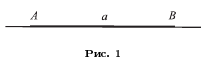
\includegraphics{mppics/ris-1}
\caption{}\label{1938/ris-1}
\bigskip
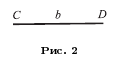
\includegraphics{mppics/ris-2}
\caption{}\label{1938/ris-2}
\bigskip
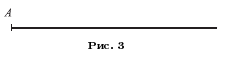
\includegraphics{mppics/ris-3}
\caption{}\label{1938/ris-3}
\end{wrapfigure}

Прямую обозначают обыкновенно двумя большими буквами, поставленными у двух каких-либо её точек.
Так, говорят:
«прямая $AB$» или «$BA$» (рис.~\ref{1938/ris-1}).

Часть прямой, ограниченная с обеих сторон, называется \index{отрезок}\textbf{отрезком};
отрезок обыкновенно обозначается двумя буквами, поставленными у его концов (отрезок $CD$, рис.~\ref{1938/ris-2}).
Иногда прямую или отрезок обозначают и одной буквой (малой);
например, говорят: «прямая $a$, отрезок $b$».

Иногда рассматривают прямую, ограниченную только с одной стороны, например в точке $A$ (рис.~\ref{1938/ris-3}).
О~такой прямой говорят, что она исходит из точки $A$;
её называют \index{луч}\textbf{лучом} или \index{полупрямая}\textbf{полупрямой}. %заменить $A$ на $E$.

\paragraph{Равенство и неравенство отрезков.}\label{1938/6}
\emph{Два отрезка равны, если они могут быть наложены один на другой так, что их концы совпадут.}
Положим, например, что мы накладываем отрезок $AB$ на
отрезок $CD$ (рис.~\ref{1938/ris-4}) так, чтобы точка $A$ совпала с точкой $C$ и чтобы прямая $AB$ пошла по прямой $CD$, если при этом концы $B$ и $D$ совпадут, то отрезки $AB$ и $CD$ равны;
в противном случае отрезки будут не равны, причём меньшим считается тот, который составит часть другого.


\begin{figure}[h!]
\centering
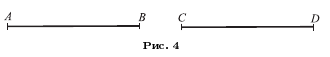
\includegraphics{mppics/ris-4}
\caption{}\label{1938/ris-4}
\end{figure}


Чтобы на какой-нибудь прямой отложить отрезок, равный данному отрезку, употребляют \textbf{циркуль} — прибор, известный учащимся из опыта.

\paragraph{Сумма отрезков.}\label{1938/7}
Суммой нескольких данных отрезков $AB$, $CD$, $EF,\dots$
(рис.~\ref{1938/ris-5}) называется такой отрезок, который получится следующим образом.
На какой-нибудь прямой берём произвольную точку $M$ и откладываем от неё отрезок $MN$, равный $AB$, затем от точки $N$ в том же направлении откладываем отрезок $NP$, равный $CD$, и отрезок $PQ$, равный $EF$.
Тогда отрезок $MQ$ и будет суммой отрезков $AB$, $CD$ и $EF$ (которые по отношению к этой сумме называются слагаемыми).
Подобным образом можно получить сумму какого угодно числа отрезков.

\begin{figure}[h!]
\centering
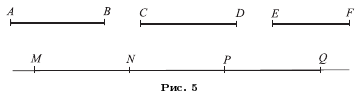
\includegraphics{mppics/ris-5}
\caption{}\label{1938/ris-5}
\end{figure}

Сумма отрезков обладает всеми свойствами суммы чисел;
так, она не зависит от порядка слагаемых (\so{переместительный закон}) и не изменяется, если некоторые слагаемые будут заменены их суммой (\so{сочетательный закон}).
Так:
\[AB+CD+EF=AB+EF+CD=EF+CD+AB=\dots\]
и
\[AB+CD+EF=AB+(CD+EF)=CD+(AB+EF)=\dots\]

\paragraph{Действия над отрезками.}\label{1938/8}
Из понятия о сумме выводятся понятия о разности отрезков, умножении и делении отрезков на отвлечённое число.
Так, разность отрезков $AB$ и $CD$ (если $AB>CD$) есть такой третий отрезок, сумма которого с $CD$ равна $AB$;
произведение отрезка $AB$ на число $3$ есть сумма трёх отрезков, из которых каждый равен $AB$;
частное от деления отрезка $AB$ на число $3$ есть третья часть $AB$ и так далее.

Если данные отрезки измерены какой-нибудь линейной единицей (например, сантиметром), и длины их выражены соответствующими числами, то длина суммы отрезков выразится суммой чисел, измеряющих эти отрезки, разность выразится разностью чисел и~т.~д.

\subsection*{Понятие об окружности}

\paragraph{Окружность.}\label{1938/9}
Если дадим циркулю произвольный раствор и, поставив одну его ножку остриём в какую-нибудь точку $O$ плоскости (рис.~\ref{1938/ris-6}), станем вращать циркуль вокруг этой точки, то другая его ножка, снабжённая карандашом или пером, прикасающимся к плоскости, опишет на плоскости непрерывную линию, все точки которой одинаково удалены от точки $O$.
Эта линия называется \index{окружность}\textbf{окружностью}, и точка $O$ — её \index{центр окружности}\textbf{центром}.
Отрезки $OA$, $OB$, $OC,\dots$, соединяющие центр с какими-нибудь точками окружности, называются радиусами.
Все радиусы одной окружности равны между собой.

\begin{wrapfigure}{R}{38 mm}
\centering
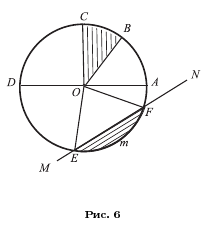
\includegraphics{mppics/ris-6}
\caption{}\label{1938/ris-6}
\end{wrapfigure}

Окружности, описанные одинаковыми радиусами, равны, так как они при совмещении их центров совмещаются всеми своими точками.
Прямая ($MN$, рис.~\ref{1938/ris-6}), проходящая через какие-нибудь две точки окружности, называется \index{секущая}\textbf{секущей}.

Отрезок ($EF$), соединяющий две какие-нибудь точки окружности, называется \index{хорда}\textbf{хордой}.

Всякая хорда ($AD$), проходящая через центр, называется \index{диаметр}\textbf{диаметром}.
Диаметр равен сумме двух радиусов, и потому все диаметры одной окружности равны между собой.
Какая-нибудь часть окружности (например, $EmF$) называется \index{дуга}\textbf{дугой}.

О хорде ($EF$), соединяющей концы какой-нибудь дуги, говорят, что она \textbf{стягивает} эту дугу.

{\sloppy

Дуга обозначается иногда знаком $\smallsmile$;
например, вместо «дуга $EmF$» пишут «${\smallsmile} EmF$».
Часть плоскости, ограниченная окружностью, называется \index{круг}\textbf{кругом}%
\footnote{Иногда слово «круг» употребляют в том же смысле, как и окружность.
Но этого следует избегать, так как употребление одного и того же термина для разных понятий может приводить к ошибкам.}%
.

}

Часть круга, заключённая между двумя радиусами (часть $COB$, покрытая штрихами на рис.~\ref{1938/ris-6}), называется \index{сектор}\textbf{сектором}, а часть, отсекаемая от круга какой-нибудь секущей (часть $EmF$), называется \index{сегмент}\textbf{сегментом}.

\begin{wrapfigure}{R}{30 mm}
\centering
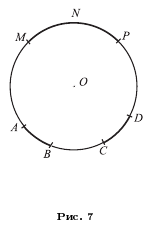
\includegraphics{mppics/ris-7}
\caption{}\label{1938/ris-7}
\end{wrapfigure}

\paragraph{Равенство и неравенство дуг.}\label{1938/10}
Две дуги одной и той же окружности (или равных окружностей) равны между собой, если они могут быть совмещены так, что их концы совпадут.
Положим, например, что мы накладываем дугу $AB$ (рис.~\ref{1938/ris-7}) на дугу $CD$ так, чтобы точка $A$ совпала с точкой $C$ и дуга $AB$ пошла по дуге $CD$;
если при этом концы $B$ и $D$ совпадут, то совпадут и все промежуточные точки этих дуг, так как они находятся на одинаковом расстоянии от центра, значит, ${\smallsmile} AB={\smallsmile} CD$;
если же $B$ и $D$ не совпадут, то дуги не равны, причём та считается меньше, которая составит часть другой.

\paragraph{Сумма дуг.}\label{1938/11}
Суммой нескольких данных дуг одинакового радиуса называется такая дуга того же радиуса, которая составлена из частей, соответственно равных данным дугам.
Так, если от произвольной точки $M$ (рис.~\ref{1938/ris-7}) окружности отложим часть $MN$, равную $AB$, и затем от точки $N$ в том же направлении отложим часть $NP$, равную $CD$, то дуга $MP$ будет суммой дуг $AB$ и $CD$.
Подобно этому можно составить сумму трёх и более дуг.

\begin{figure}[h!]
\centering
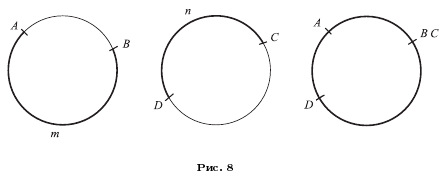
\includegraphics{mppics/ris-8}
\caption{}\label{1938/ris-8}
\end{figure}

При сложении дуг одинакового радиуса их сумма может не уместиться на одной окружности, одна из дуг может частично покрыть другую.
В таком случае суммой дуг будет являться дуга, б\'{о}льшая целой окружности.
Так, например, при сложении дуги $AmB$ с дугой $CnD$ (рис.~\ref{1938/ris-8}) получаем дугу, состоящую из целой окружности и дуги $AD$.


Сумма дуг, как и сумма отрезков, обладает свойствами \textbf{переместительным} и \textbf{сочетательным}.

Из понятия о сумме дуг выводятся понятия о разности дуг, умножении и делении дуги на отвлечённое число, так же как и для отрезков.


\paragraph{Разделение геометрии.}\label{1938/12}
Геометрия разделяется на две части:
\textbf{планиметрию} и \textbf{стереометрию}.
Первая рассматривает свойства таких фигур, все части которых помещаются на одной плоскости;
вторая — свойства таких фигур, у которых не все части помещаются на одной плоскости.



%\part{Планиметрия}

\chapter{Прямая линия}


\section{Углы} 

\subsection*{Предварительные понятия}

\paragraph{Угол.}\label{1938/13}
Фигура, образованная двумя лучами, исходящими из одной точки, называется \index{угол}\textbf{углом}.
Полупрямые, образующие угол, называются \index{сторона угла}\textbf{сторонами}, а точка, из которой они исходят, — \index{вершина угла}\textbf{вершиной угла}.
Стороны следует представлять себе неограниченно продолженными от вершины.

\begin{wrapfigure}{R}{31 mm}
\centering
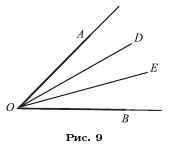
\includegraphics{mppics/ris-9}
\caption{}\label{1938/ris-9}
\end{wrapfigure}

Угол обыкновенно обозначается тремя большими буквами, из которых средняя ставится у вершины, а крайние — у каких-нибудь точек сторон;
например, говорят:
«угол $AOB$» или «угол $BOA$» (рис.~\ref{1938/ris-9}).
Но можно обозначить угол и одной буквой, поставленной у вершины, если при этой вершине нет других углов.
Мы иногда будем обозначать угол цифрой, поставленной внутри угла около вершины.

Стороны угла разделяют всю плоскость, в которой лежит этот угол, на две области.
Одна из них называется \index{внутренняя область угла}\textbf{внутренней областью угла}, другая — \index{внешняя область угла}\textbf{внешней его областью}.
Обычно внутренней областью считается та, в которой целиком помещается отрезок, соединяющей две любые точки, взятые на сторонах угла, например точки $A$ и $B$ на сторонах угла $AOB$ (рис.~\ref{1938/ris-9}).
Но иногда приходится считать внутренней областью угла другую часть плоскости.
В этих случаях обычно делается специальное указание, какая область плоскости считается внутренней областью угла.

На рис.~\ref{1938/ris-10} представлены раздельно оба случая.
Внутренней областью угла в каждом случае служит заштрихованная часть плоскости.
Если из вершины угла (рис.~\ref{1938/ris-9}) проведём внутри него какие-нибудь прямые $OD, OE,\dots$, то образовавшиеся при этом углы $AOD$, $DOE$, $EOB,\dots$, рассматриваются как части угла $AOB$.

\begin{figure}[h!]
\centering
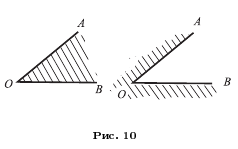
\includegraphics{mppics/ris-10}
\caption{}\label{1938/ris-10}
\end{figure}

Слово «угол» при записи заменяется часто знаком $\angle$.
Например, вместо «угол $AOB$» обычно пишут:
$\angle AOB$.

\paragraph{Равенство и неравенство углов.}\label{1938/14}
В соответствии с общим определением равенства геометрических фигур (§~\ref{1938/1}) \emph{два угла считаются равными, если при наложении они могут совместиться.}

\begin{figure}[h]
\centering
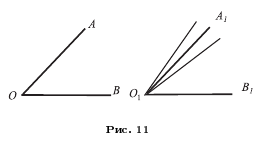
\includegraphics{mppics/ris-11}
\caption{}\label{1938/ris-11}
\end{figure}

Положим, например, что мы накладываем угол $AOB$ на угол $A_1O_1B_1$ (рис.~\ref{1938/ris-11}) так, чтобы вершина $O$ совпала с $O_1$, сторона $OB$ пошла по $O_1B_1$ и чтобы внутренние области обоих углов были расположены по одну сторону от прямой $O_1B_1$.
Если при этом сторона $OA$ совместится с $O_1A_1$, то углы равны;
если же $OA$ пойдёт внутри угла $A_1O_1B_1$ или же вне его, то углы не равны, причём тот из них будет меньше, который составит часть другого угла.

\begin{figure}[h!]
\centering
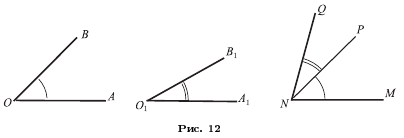
\includegraphics{mppics/ris-12}
\caption{}\label{1938/ris-12}
\end{figure}

\paragraph{Сумма углов.}\label{1938/15}
Суммой углов $AOB$ и $A_1O_1B_1$ (рис.~\ref{1938/ris-12}) называется такой угол, который получится следующим образом.
Строим угол $MNP$, равный первому данному углу $AOB$, и к нему пристраиваем угол $PNQ$, равный другому данному углу $A_1O_1B_1$ так, чтобы у обоих углов оказалась общая вершина $N$ и общая сторона $NP$ и чтобы внутренние области углов были расположены по разные стороны от общей стороны $NP$.
Тогда угол $MNQ$, называется суммой углов $AOB$ и $A_1O_1B_1$.
Внутренней областью этого угла служит та область плоскости, которая образована совокупностью внутренних областей складываемых углов.
Это та область, в которой лежит общая сторона ($NP$) складываемых углов.
Подобным образом может быть составлена сумма трёх и более углов.

\begin{wrapfigure}{R}{50 mm}
\centering
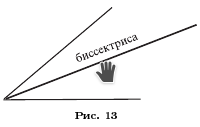
\includegraphics{mppics/ris-13}
\caption{}\label{1938/ris-13}
\bigskip
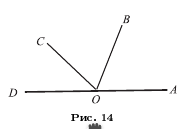
\includegraphics{mppics/ris-14}
\caption{}\label{1938/ris-14}
\end{wrapfigure}

Сумма углов, как и сумма отрезков, обладает свойствами переместительным и сочетательным.
Часто приходится говорить о такой полупрямой, которая делит данный угол пополам;
такой полупрямой дали особое название:
\index{биссектриса}\textbf{биссектриса} (рис.~\ref{1938/ris-13}).


\paragraph{Расширение понятия об угле.}\label{1938/16}
При нахождении суммы углов могут представиться некоторые особые случаи, которые полезно рассмотреть отдельно.

1.
Может случиться, что после сложения нескольких углов, например трёх:
$AOB$, $BOC$ и $COD$ (рис.~\ref{1938/ris-14}), сторона $OD$ угла $COD$ составит продолжение стороны $OA$ угла $AOB$.
Мы получим тогда фигуру, образованную двумя полупрямыми ($OA$ и $OD$), исходящими из одной точки ($O$) и составляющими продолжение одна другой.
Такую фигуру принято тоже называть углом (\index{развёрнутый угол}\textbf{развёрнутым}).

2.
Может случиться, что после сложения нескольких углов, например пяти углов:
$AOB$, $BOC$, $COD$, $DOE$ и $EOA$ (рис.~\ref{1938/ris-15}), сторона $OA$ угла $EOA$ совместится со стороной $OA$ угла $AOB$.

\begin{wrapfigure}{R}{40 mm}
\centering
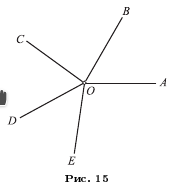
\includegraphics{mppics/ris-15}
\caption{}\label{1938/ris-15}
\end{wrapfigure}

Фигура, образованная такими совпавшими полупрямыми (рассматриваемая вместе со всей плоскостью, расположенной вокруг общей вершины $O$), также называется углом (\index{полный угол}\textbf{полным}).


3.
Наконец, может случиться, что, строя сумму углов, мы не только заполним всю плоскость вокруг их общей вершины, но даже будем вынуждены налагать углы один на другой, покрывая плоскость вокруг общей вершины во второй раз, в третий раз и~т.~д.
Такая сумма углов равна одному полному углу, сложенному с некоторым углом, или равна двум полным углам, сложенным с некоторым углом, и~т.~д.

\subsection*{Измерение углов}


\paragraph{Центральный угол.}\label{1938/17}
Угол ($AOB$, рис.~\ref{1938/ris-16}), образованный двумя радиусами окружности, называется центральным углом;
о таком угле и дуге, заключённой между его сторонами, говорят, что они \textbf{соответствуют} друг другу.

\begin{wrapfigure}{r}{30 mm}
\vskip-4mm
\centering
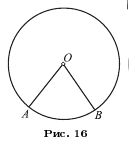
\includegraphics{mppics/ris-16}
\caption{}\label{1938/ris-16}
\bigskip
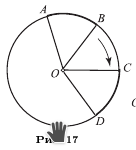
\includegraphics{mppics/ris-17}
\caption{}\label{1938/ris-17}
\end{wrapfigure}

Центральные углы по отношению к соответствующим им дугам обладают следующими двумя свойствами.

\textbf{\emph{В одном круге или в равных кругах.}}

1) \textbf{\emph{Если центральные углы равны, то и соответствующие им дуги равны.}}

2) Обратно.
\textbf{\emph{Если дуги равны, то и соответствующие им центральные углы равны.}}


Пусть $\angle AOB=\angle COD$ (рис.~\ref{1938/ris-17}), покажем, что дуги $AB$ и $CD$ также равны.
Вообразим, что сектор $AOB$ мы повернули вокруг центра $O$ в направлении, указанном стрелкой, настолько, чтобы радиус $OA$ совпал с $OC$.
Тогда, вследствие равенства углов, радиус $OB$ совместится с $OD$;
значит, совместятся и дуги $AB$ и $CD$, то есть
они будут равны.

Второе свойство также легко обнаружить наложением.

\paragraph{Градусы дуговой и угловой.}\label{1938/18}
Вообразим, что какая-нибудь окружность разделена на 360 равных частей и ко всем точкам деления проведены радиусы.
Тогда вокруг центра образуются 360 центральных углов, которые, как соответствующие равным дугам, должны быть равны между собой.
Каждая из полученных таким образом на окружности дуг называется \index{градус}\textbf{дуговым градусом}, а каждый из образовавшихся при центре углов называется \textbf{угловым градусом}.
Значит, можно сказать, что дуговой градус есть $\tfrac1{360}$ часть окружности,
а угловой градус есть центральный угол, соответствующий дуговому градусу.

Градусы (дуговые и угловые) подразделяются ещё на 60 равных частей, называемых \index{минута}\textbf{минутами}, а минуты подразделяются ещё на 60 равных частей, называемых \index{секунда}\textbf{секундами}.

\begin{figure}[h!]
\centering
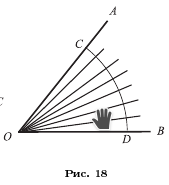
\includegraphics{mppics/ris-18}
\caption{}\label{1938/ris-18}
\end{figure}

Пусть $AOB$ есть какой-нибудь угол (рис.~\ref{1938/ris-18}).
Опишем между его сторонами с центром в вершине $O$ дугу $CD$ произвольного радиуса;
тогда угол $AOB$ будет центральным углом, соответствующим дуге $CD$.
При этом угол измеряется соответствующей ему дугой; то есть в угле содержится столько угловых градусов, минут и секунд, сколько в соответствующей ему дуге содержится дуговых градусов, минут и секунд.
Если, например, в дуге $CD$ содержится $20{,}57$ градусов или, что то же самое, 20 градусов 34 минут 12 секунд,%
\footnote{Поскольку \[20{,}57=20\tfrac{57}{100}=20+\tfrac{34}{60}+\tfrac{12}{60\cdot 60}.\]}
 то и в угле $AOB$ заключается 20 градусов 34 минут 12 секунд угловых, что принято выражать так:
$\angle AOB = 20{,}57\degree = 20\degree 34'12''$ обозначая знаками $\degree$, $'$ и $''$ соответственно градусы, минуты и секунды.

Величина углового градуса не зависит от радиуса окружности.
Действительно, если сложить 360 угловых градусов по правилу, указанному в §~\ref{1938/15}, то получим полный угол при центре окружности.
Каков бы ни был радиус окружности, этот полный угол будет один и тот же.
Значит, можно сказать, что угловой градус составляет $\tfrac1{360}$ часть полного угла.
Это мера угла, вполне определяющая его величину независимо от радиуса окружности.
Число угловых градусов в данном угле принимают за меру наклона одной стороны угла к другой.

Поскольку число 360 имеет много делителей,
градусы удобны для работы с дробными долями полного угла.
Тем не менее основной единицей измерения углов считается \textbf{радиан};
он будет определён в §~\ref{1938/241}. 
Кроме градусов и радиан употребляются и другие единицы для измерения углов, например \textbf{прямой угол}, \textbf{оборот} равный полному углу и
\textbf{град} равный сотой доле прямого угла.
%!!!существенное изменение

\paragraph{Транспортир.}\label{1938/20}
Для измерения углов употребляется особый прибор — \index{транспортир}\textbf{транспортир}.
Этот прибор (рис.~\ref{1938/ris-19}) представляет собой полукруг, дуга которого разделена на $180\degree $.
Чтобы измерить угол $DCE$, накладывают на него прибор так, чтобы центр полукруга совпадал с вершиной угла, а радиус $CB$ был расположен по стороне $CE$.
Тогда число градусов, содержащееся в дуге, заключённой между сторонами угла $DCE$, покажет величину его.
При помощи транспортира можно также начертить угол, содержащий данное число градусов.

\begin{figure}[h!]
\centering
\ \ \includegraphics{mppics/transportir-19}
\caption{}\label{1938/ris-19}
\end{figure}

\paragraph{Прямой, острый и тупой углы.}\label{1938/21}
Угол в $90\degree$ (составляющий, следовательно, половину развёрнутого угла или четверть полного угла) называют \index{прямой угол}\textbf{прямым углом};
угол, меньший прямого, называют \index{острый угол}\textbf{острым}, а угол, больший прямого, но меньший развёрнутого, называют \index{тупой угол}\textbf{тупым} (рис.~\ref{1938/ris-20})

\begin{figure}[h!]
\centering
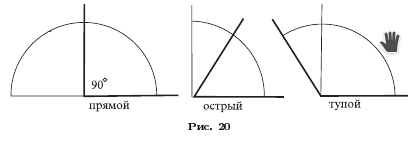
\includegraphics{mppics/ris-20}
\caption{}\label{1938/ris-20}
\end{figure}

Конечно, \textbf{\emph{все прямые углы}}, как содержащие одинаковое число градусов, \textbf{\emph{равны между собой}}.
На чертежах прямой угол принято обозначать квадратиком, как показано на рис.~\ref{1938/ris-20}.

\subsection*{Смежные и вертикальные углы}

\begin{wrapfigure}{R}{40 mm}
\centering
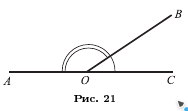
\includegraphics{mppics/ris-21}
\caption{}\label{1938/ris-21}
\bigskip
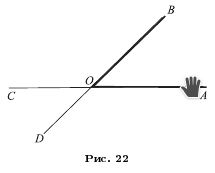
\includegraphics{mppics/ris-22}
\caption{}\label{1938/ris-22}
\bigskip
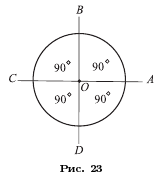
\includegraphics{mppics/ris-23}
\caption{}\label{1938/ris-23}
\end{wrapfigure}

\paragraph{Смежные углы и их свойства.}\label{1938/22}
Два угла ($AOB$ и $BOC$, рис.~\ref{1938/ris-21}) называются \index{смежные углы}\textbf{смежными}, если одна сторона у них общая, а две другие стороны составляют продолжение одна другой.

Так как такие углы в сумме составляют развёрнутый угол, то \textbf{\emph{сумма двух смежных углов равна $\bm{180\degree}$}}.

Для каждого данного угла можно построить два смежных с ним угла.
Например, для угла $AOB$ (рис.~\ref{1938/ris-22}), продолжив сторону $AO$, мы получим один смежный угол $AOD$.
\emph{Два угла, $BOC$ и $AOD$, смежные с одним и тем же углом $AOB$, равны между собой,} так как каждый из них дополняет угол $AOB$ до $180\degree$.

Если угол $AOB$ прямой (рис.~\ref{1938/ris-23}), то есть если он содержит $90\degree$, то и каждый из смежных с ним углов $COB$ и $AOB$ должен быть также прямой, так как он содержит в себе $180\degree-90\degree$, то есть $90\degree$;
четвёртый угол $COB$ тоже должен быть прямым, так как три угла $AOB$, $BOC$ и $AOB$ составляют в сумме $270\degree$ и, следовательно, от $360\degree$ на долю четвёртого угла $COB$ остаётся тоже $90\degree$.
Таким образом:
\emph{если при пересечении двух прямых \emph{($AC$ и $BD$, рис.~\ref{1938/ris-23})} один из четырёх углов окажется прямой, то и остальные три угла должны быть прямые.}

\paragraph{Перпендикуляр и наклонная.}\label{1938/23}
Общая сторона ($OB$) двух смежных углов называется \index{наклонная}\textbf{наклонной} к прямой ($AC$), на которой лежат две другие стороны, в том случае, когда смежные углы не равны между собой (рис.~\ref{1938/ris-24});
в том же случае, когда смежные углы равны (рис.~\ref{1938/ris-25}) и когда, следовательно, каждый из углов есть прямой, общая сторона называется \index{перпендикуляр}\textbf{перпендикуляром} к прямой, на которой лежат две другие стороны.
Общая вершина ($O$) в первом случае называется \index{основание наклонной}\textbf{основанием наклонной}, во втором случае — \textbf{основанием перпендикуляра}.

\begin{figure}
\begin{minipage}{.48\textwidth}
\centering
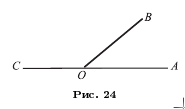
\includegraphics{mppics/ris-24}
\caption{}\label{1938/ris-24}
\end{minipage}\hfill
\begin{minipage}{.48\textwidth}
\centering
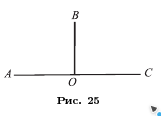
\includegraphics{mppics/ris-25}
\caption{}\label{1938/ris-25}
\end{minipage}
\end{figure}

Две прямые ($AC$ и $BD$, рис.~\ref{1938/ris-23}), пересекающиеся между собой под прямым углом, называются взаимно \index{перпендикулярные прямые}\textbf{перпендикулярными}.
Что прямая $AC$ перпендикулярна к прямой $BD$, записывают так: $AC\perp BD$.

\smallskip

\so{Замечания}.
1) Если перпендикуляр к прямой $AC$ (рис.~\ref{1938/ris-25}) приходится проводить из точки $O$, лежащей на этой прямой, то говорят, что этот перпендикуляр надо «восстановить» к прямой $AC$, а если требуется перпендикуляр провести из точки $B$, лежащей вне прямой, то говорят, что его надо \so{опустить} на прямую (всё равно:
вниз или вверх, или вбок).

\begin{wrapfigure}[11]{r}{38 mm}
\centering
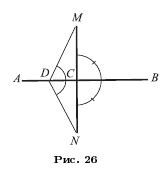
\includegraphics{mppics/ris-26}
\caption{}\label{1938/ris-26}
\end{wrapfigure}

2) Очевидно, что из всякой точки данной прямой можно к этой прямой восстановить перпендикуляр и притом только один.

\paragraph{}\label{1938/24}
Докажем, что \textbf{\emph{из всякой точки, лежащей вне прямой, можно опустить на эту прямую перпендикуляр и только один}}.

Пусть дана какая-нибудь прямая $AB$ (рис.~\ref{1938/ris-26}) и вне её произвольная точка $M$;
требуется показать, что, во-первых, из этой точки можно опустить на прямую $AB$ перпендикуляр и, во-вторых, что этот перпендикуляр может быть только один.

Вообразим, что мы перегнули чертёж;
по прямой $AB$ так, чтобы верхняя его часть упала на нижнюю.
Тогда точка $M$ займёт некоторое положение $N$.
Отметив это положение, приведём чертёж;
в прежний вид и затем соединим точки $M$ и $N$ прямой.
Убедимся, что полученная прямая $MN$ перпендикулярна к $AB$, а всякая иная прямая, исходящая из $M$, например $MD$, не перпендикулярна к $AB$.
Для этого перегнём чертёж вторично.
Тогда точка $M$ снова совместится с $N$, а точки $C$ и $D$ останутся на своих местах;
следовательно, прямая $MC$ совпадёт с $NC$, а $MD$ с $ND$.
Из этого следует, что $\angle MCB = \angle BCN$ и $\angle MDC = \angle CDN$.

Но углы $MCB$ и $BCN$ смежные и, как теперь видим, равные;
следовательно, каждый из них есть \so{прямой}, а потому $MN\z\perp AB$.
Так как линия $MDN$ не прямая (потому что не может быть двух различных прямых, соединяющих точки $M$ и $N$), то сумма двух равных углов $MDC$ и $CDN$ \so{не равна} $180\degree$;
поэтому угол $MDC$ не есть прямой, и, значит, $MD$ не перпендикулярна к $AB$.
Таким образом, другого перпендикуляра из точки $M$ на прямую $AB$ опустить нельзя.

\begin{wrapfigure}[19]{r}{43 mm}
\vskip-6mm
\centering
%\begin{lpic}[t(-6 mm),b(0 mm),r(0 mm),l(0 mm)]{geogebra/ugolnik(1)}
%\lbl[b]{2,6;$A$}
%\lbl[b]{42,6;$B$}
%\lbl[rb]{16.5,6;$C$}
%\lbl[rb]{16.5,25;$D$}
%\lbl[r]{16.5,36;$E$}
%\end{lpic}
%\caption{}\label{1938/ris-27}
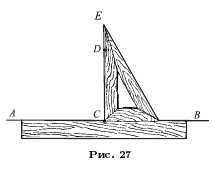
\includegraphics{mppics/ris-27}
\caption{}\label{1938/ris-27}
\bigskip
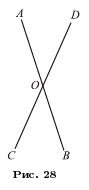
\includegraphics{mppics/ris-28}
\caption{}\label{1938/ris-28}
\end{wrapfigure}

\paragraph{Угольник.}\label{1938/25} 
Для построения перпендикуляра к данной прямой очень удобен угольник — чертёжный инструмент в виде треугольника у которого один из углов делается прямым.
Чтобы провести перпендикуляр к прямой $AB$ (рис.~\ref{1938/ris-27}) через точку $D$, взятую вне прямой, приставляют линейку к прямой $AB$, к линейке угольник, а затем, придерживая линейку рукой, двигают угольник вдоль линейки до тех пор, пока другая сторона прямого угла не пройдёт через точку $D$, затем проводят прямую $CE$.
Точно также поступают если точка $D$ лежит на прямой $AB$.

\paragraph{Вертикальные углы и их свойство.}\label{1938/26}
Два угла называются \index{вертикальные углы}\textbf{вертикальными}, если стороны одного составляют продолжение сторон другого.
Так, при пересечении двух прямых $AB$ и $CD$ (рис.~\ref{1938/ris-28}) образуются две пары вертикальных углов:
$AOD$ и $COB$, $AOC$ и $DOB$ (и четыре пары смежных углов).

\textbf{\emph{Два вертикальных угла равны между собой}} (например, $\angle AOD = \angle BOC$), так как каждый из них есть смежный с одним и тем же углом (с~$\angle DOB$ или с~$\angle AOC$), а такие углы, как мы видели (§~\ref{1938/22}), равны друг другу.

\paragraph{Замечания об углах, имеющих общую вершину.}\label{1938/27}
Об углах, имеющих общую вершину, полезно помнить следующие простые истины.

1) \emph{Если сумма нескольких углов ($AOB$, $BOC$, $COD$, $DOE$, рис.~\ref{1938/ris-29}), имеющих общую вершину, составляет развёрнутый угол, то она равна $180\degree$.}

2) \emph{Если сумма нескольких углов ($AOB$, $BOC$, $COD$, $DOE$, $EOA$ рис.~\ref{1938/ris-30}), имеющих общую вершину, составляет полный угол, то она равна  $360\degree$.}

3) \emph{Если два угла ($AOB$ и $BOC$, рис.~\ref{1938/ris-24}) имеют общую вершину ($O$) и общую сторону ($OB$) и в сумме составляют $180\degree$, то их две другие стороны ($AO$ и $OC$) составляют продолжение одна другой} (то есть такие углы будут смежными).

\begin{figure}
\begin{minipage}{.48\textwidth}
\centering
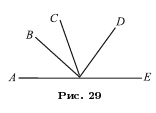
\includegraphics{mppics/ris-29}
\caption{}\label{1938/ris-29}
\end{minipage}\hfill
\begin{minipage}{.48\textwidth}
\centering
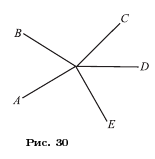
\includegraphics{mppics/ris-30}
\caption{}\label{1938/ris-30}
\end{minipage}
\end{figure}


\subsection*{Упражнения}

\begin{enumerate}

 \item
Некоторый угол равен $38\degree 20'$;
найти величину смежного с ним угла.

 \item
Два угла $ABC$ и $CBD$, имея общую вершину $B$ и общую сторону $BC$, расположены так, что они не покрывают друг друга;
угол $ABC = 100\degree20'$ , а угол $CBD = 79\degree 40'$.
Составляют ли стороны $AB$ и $BD$ прямую или ломаную.

 \item
Построить какой-нибудь угол и при помощи транспортира и линейки провести его биссектрису.

\end{enumerate}

\smallskip
\so{Доказать}, что:

\begin{enumerate}[resume]
 \item
Биссектрисы двух смежных углов взаимно перпендикулярны.

 \item
Биссектрисы двух вертикальных углов составляют продолжение одна другой.

 \item
Если при точке $O$ прямой $AB$ (рис.~\ref{1938/ris-28}) построим по разные стороны от $AB$ равные углы $AOB$ и $BOC$, то стороны их $OD$ и $OC$ составляют одну прямую.

 \item
Если из точки $O$ (рис.~\ref{1938/ris-28}) проведём полупрямые $OA$, $OB$, $OB$, $OC$ так, что $\angle AOC = \angle DOB$ и $\angle AOD=\angle COD$, то $OD$ есть продолжение $OA$ и $OB$ есть продолжение $OC$.

\smallskip
\so{Указание}.
Надо применить §~\ref{1938/27}, 2 и 3.

\end{enumerate}

\section{Математические предложения}



\paragraph{Теоремы, аксиомы, определения.}\label{1938/28}
Из того, что было изложено, можно заключить, что некоторые геометрические истины мы считаем вполне очевидными (например, свойства плоскости и прямой в §§~\ref{1938/3} и \ref{1938/4}), а другие устанавливаем путём рассуждений (например, свойства смежных углов в §~\ref{1938/22} и вертикальных в §~\ref{1938/26}).
Такие рассуждения являются в геометрии главным средством обнаружить свойства геометрических фигур.
Поэтому для дальнейшего полезно заранее познакомиться с теми видами рассуждений, которые применяются в геометрии.
Все истины, которые устанавливаются в геометрии, выражаются в виде предложений.

Эти предложения бывают следующих видов.

\textbf{Определения.}
Определениями называют предложения, в которых разъясняется, какой смысл придают тому или другому названию или выражению.
Например, мы уже встречали определения центрального угла, прямого угла и перпендикуляра.

\textbf{Аксиомы.}
Аксиомами называют истины, которые принимаются без доказательства.
Таковы, например, предложения, встречавшиеся нам ранее (§~\ref{1938/4}):
через всякие две точки можно провести прямую и притом только одну;
если две точки прямой лежат в данной плоскости, то и все точки этой прямой лежат в той же плоскости.

Укажем ещё следующие аксиомы, относящиеся ко всякого рода величинам:

если две величины равны порознь одной и той же третьей величине, то они равны и между собой.

если к равным величинам прибавим поровну или от равных величин отнимем поровну, то равенство не нарушится.

если к неравным величинам прибавим поровну или от неравных величин отнимем поровну, то смысл неравенства не изменится, то есть б\'{о}льшая величина останется б\'{о}льшей.

\textbf{Теоремы.}
Теоремами называются предложения, истинность которых обнаруживается только после некоторого рассуждения (доказательства).
Примером могут служить следующие предложения.

если в одном круге или в равных кругах центральные углы равны, то и соответствующие им дуги равны.

если при пересечении двух прямых между собой один из четырёх углов окажется прямой, то и остальные три угла прямые.

\textbf{Следствия.}
Следствиями называются предложения, которые составляют непосредственный вывод из аксиомы или из теоремы.
Например, из аксиомы:
«через две точки можно провести только одну прямую» следует, что «две прямые могут пересечься только в одной точке».

\paragraph{Состав теоремы.}\label{1938/29}
Во всякой теореме можно различить две части:
условие и заключение.
\textbf{Условие} выражает то, что предполагается данным;
\textbf{заключение} — то, что требуется доказать.
Например, в теореме:
«если центральные углы равны, то и соответствующие им дуги равны» условием служит первая часть теоремы:
«если центральные углы равны», а заключением — вторая часть:
«то и соответствующие им дуги равны»;
другими словами, нам дано (нам известно), что центральные углы равны, а требуется доказать, что при этом условии и соответствующие дуги также равны.

Условие и заключение теоремы могут иногда состоять из нескольких отдельных условий и заключений;
например, в теореме:
«если число делится на 2 и на 3, то оно разделится и на 6» условие состоит из двух частей:
«если число делится на 2» и «если число делится на 3».

Полезно заметить, что всякую теорему можно подробно выразить словами так, что её условие будет начинаться словом «если», а заключение — словом «то».
Например, теорему:
«вертикальные углы равны» можно подробнее высказать так:
«если два угла вертикальные, то они равны».

\paragraph{Обратная теорема.}\label{1938/30}
Теоремой, обратной данной теореме, называется такая, в которой условием поставлено заключение (или часть заключения), а заключением — условие (или часть условия) данной теоремы.
Например, следующие две теоремы обратны друг другу.

\medskip

\noindent
\begin{tabular}{ p{.47\textwidth}| p{.47\textwidth} }
\textbf{\emph{Если центральные углы равны, то и соответствующие им дуги равны.}}
&
\textbf{\emph{Если дуги равны, то и соответствующие им центральные углы равны.}}
\end{tabular}

\medskip

Если одну из этих теорем назовём \textbf{прямой}, то другую следует назвать обратной.
В этом примере обе теоремы, и прямая, и обратная, оказываются верными.
Но так бывает не всегда.
Например, теорема:
«если два угла вертикальные, то они равны» верна, но обратное предложение:
«если два угла равны, то они вертикальные» неверно.

В самом деле, допустим, что в каком-либо углу проведена его биссектриса (рис.~\ref{1938/ris-13}).
Она разделит данный угол на два меньших угла.
Эти углы будут равны между собой, но они не будут вертикальными.

\paragraph{Противоположная теорема.}\label{1938/31}
Теоремой, противоположной данной теореме, называется такая, условие и заключение которой представляют отрицание условия и заключения данной теоремы.
Например, теореме:
«если сумма цифр делится на 9, то число делится на 9» соответствует такая противоположная:
«если сумма цифр не делится на 9, то число не делится на 9».

И здесь должно заметить, что верность прямой теоремы ещё не служит доказательством верности противоположной:
например, противоположное предложение:
«если каждое слагаемое не делится на одно и то же число, то и сумма не разделится на это число» — неверно, тогда как прямое предложение верно.

\paragraph{Зависимость между теоремами: прямой, обратной и противоположной.}\label{1938/32}
Для лучшего уяснения этой зависимости выразим теоремы сокращённо так (буквой $A$ мы обозначим условие теоремы, а буквой $B$ — её заключение).

1) \textbf{Прямая:}
если есть $A$, то есть и $B$.

2) \textbf{Обратная:}
если есть $B$, то есть и $A$.

3) \textbf{Противоположная прямой:}
если нет $A$, то нет и $B$.

4) \textbf{Противоположная обратной:}
если нет $B$, то нет и $A$.

Рассматривая эти предложения, легко заметить, что первое из них находится в таком же отношении к четвёртому, как второе к третьему, а именно:
предложения первое и четвёртое обратимы одно в другое, равно как второе и третье.
Действительно, из предложения:
«если есть $A$, то есть и $B$» непосредственно следует:
«если нет $B$, то нет и $A$» (так как если бы $A$ было, то, согласно первому предложению, было бы и $B$);
обратно, из предложения:
«если нет $B$, то нет и $A$» выводим:
«если есть $A$, то есть и $B$» (так как если бы $B$ не было, то не было бы и $A$).
Совершенно так же убедимся, что из второго предложения следует третье, и наоборот.

Таким образом, чтобы иметь уверенность в справедливости всех четырёх теорем, нет надобности доказывать каждую из них отдельно, а достаточно ограничиться доказательством только двух:
прямой и обратной, или прямой и противоположной.

\section{Треугольники}

\subsection*{Понятие о многоугольнике и треугольнике}

\paragraph{Ломаная линия.}\label{1938/33}
Линия, образуемая отрезками, не лежащих на одной прямой и расположенных так, что конец первого служит началом второго, конец второго — началом третьего и~т.~д., называется \index{ломаная}\textbf{ломаной линией} (рис.~\ref{1938/ris-31} и \ref{1938/ris-32}).
Эти отрезки называются сторонами ломаной, а вершины углов, образуемых соседними отрезками, — \index{вершина ломаной}\textbf{вершинами} её.
Ломаная линия обозначается рядом букв, поставленных у её вершин и концов;
например говорят:
ломаная $ABCDE$.
Ломаная линия называется \index{ломаная!выпуклая ломаная}\textbf{выпуклой}, если она вся расположена по одну сторону от каждого входящего в её состав отрезка, продолженного неограниченно в обе стороны.
Такова, например, линия, изображённая на рис.~\ref{1938/ris-31}, тогда как ломаная на рис.~\ref{1938/ris-32} не будет выпуклой (она расположена не по одну сторону от прямой $BC$), рис.~\ref{1938/ris-31}.

\begin{figure}[h!]
\begin{minipage}{.48\textwidth}
\centering
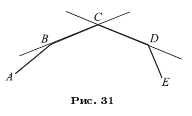
\includegraphics{mppics/ris-31}
\caption{}\label{1938/ris-31}
\end{minipage}\hfill
\begin{minipage}{.48\textwidth}
\centering
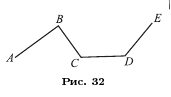
\includegraphics{mppics/ris-32}
\caption{}\label{1938/ris-32}
\end{minipage}
\end{figure}

Когда концы ломаной сходятся в одну точку, то она называется \so{замкнутой} (например, линия $ABCDE$ на рис.~\ref{1938/ris-33}).

\paragraph{Многоугольник.}\label{1938/34}
Фигура, образованная замкнутой ломаной линией вместе с частью плоскости, ограниченной этой линией, называется многоугольником (рис.~\ref{1938/ris-33}).
Стороны этой ломаной называются \index{сторона многоугольника}\textbf{сторонами} многоугольника, углы, составленные каждыми двумя соседними сторонами, — \index{угол многоугольника}\textbf{углами} многоугольника, а их вершины — \index{вершина многоугольника}\textbf{вершинами} его.

\begin{figure}[h!]
\centering
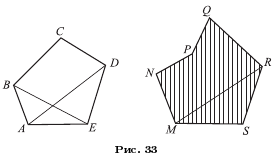
\includegraphics{mppics/ris-33}
\caption{}\label{1938/ris-33}
\end{figure}

При этом внутренней областью угла многоугольника считается (рис.~\ref{1938/ris-33}) та, к которой принадлежит непосредственно примыкающая к вершине внутренняя область самого многоугольника.
Так, для многоугольника $MNPQRS$ (рис.~\ref{1938/ris-33}) углом при вершине $P$ является угол, больший двух прямых (с заштрихованной внутренней областью).
Сама ломаная линия, ограничивающая многоугольник, называется \index{контур многоугольника}\textbf{контуром} его, а отрезок, равный сумме всех его сторон, — \index{периметр}\textbf{периметром}.

Многоугольник называется \index{выпуклый многоугольник}\textbf{выпуклым}, если он ограничен выпуклой ломаной линией;
таков, например, многоугольник $ABCDE$, изображённый на рис.~\ref{1938/ris-33} (многоугольник $MNPQRS$ нельзя назвать выпуклым);
мы будем рассматривать, главным образом, выпуклые многоугольники.

Всякая прямая (как $AD$, $BE$, $MR,\dots$, рис.~\ref{1938/ris-33}), которая соединяет вершины двух углов многоугольника, не прилежащих к одной стороне, называется \index{диагональ}\textbf{диагональю} многоугольника.

Наименьшее число сторон в многоугольнике — три.
По числу сторон многоугольник называется \textbf{треугольником}, \textbf{четырёхугольником}, \textbf{пятиугольником} и~т.~д; многоугольник с $n$ сторонами называется \index{$n$-угольник}\textbf{$\bm{n}$-угольником}. 

Для краткости «треугольник» обозначается символом $\triangle$;
например вместо «треугольник $ABC$» пишут «$\triangle ABC$».

\paragraph{Типы треугольников.}\label{1938/35}
Треугольники разделяются по сравнительной длине их сторон или по величине их углов.
Относительно длины сторон они бывают:
\index{разносторонний треугольник}\textbf{разносторонние} (рис.~\ref{1938/ris-34}), когда все стороны различной длины, и \index{равнобедренный треугольник}\textbf{равнобедренные} (рис.~\ref{1938/ris-35}), когда две стороны одинаковы;
в частности, равнобедренный треугольник называется \index{равносторонний треугольник}\textbf{равносторонним} (рис.~\ref{1938/ris-36}), когда все три его стороны равны между собой.

\begin{figure}[h!]
\begin{minipage}{.32\textwidth}
\centering
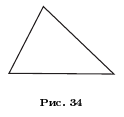
\includegraphics{mppics/ris-34}
\caption{}\label{1938/ris-34}
\end{minipage}\hfill
\begin{minipage}{.32\textwidth}
\centering
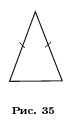
\includegraphics{mppics/ris-35}
\caption{}\label{1938/ris-35}
\end{minipage}\hfill
\begin{minipage}{.32\textwidth}
\centering
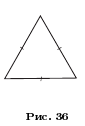
\includegraphics{mppics/ris-36}
\caption{}\label{1938/ris-36}
\end{minipage}
\\
\begin{minipage}{.48\textwidth}
\centering
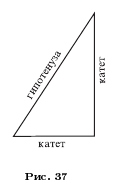
\includegraphics{mppics/ris-37}
\caption{}\label{1938/ris-37}
\end{minipage}
\hfill
\begin{minipage}{.48\textwidth}
\centering
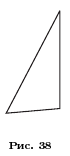
\includegraphics{mppics/ris-38}
\caption{}\label{1938/ris-38}
\end{minipage}
\end{figure}

Относительно величины углов треугольники бывают:
\index{остроугольный треугольник}\textbf{остроугольные} (рис.~\ref{1938/ris-34}), когда все углы острые, \index{прямоугольный треугольник}\textbf{прямоугольные} (рис.~\ref{1938/ris-37}), когда в числе углов есть прямой, и \index{тупоугольный треугольник}\textbf{тупоугольные} (рис.~\ref{1938/ris-38}), когда в числе углов есть тупой.

В прямоугольном треугольнике стороны, образующие прямой угол, называются \index{катет}\textbf{катетами}, а сторона, лежащая против прямого угла, — \index{гипотенуза}\textbf{гипотенузой}.

\paragraph{Основные линии в треугольнике.}\label{1938/36}
Одну из сторон треугольника иногда называют \index{основание!основание треугольника}\textbf{основанием}, тогда вершину противоположного угла называют \index{вершина!вершина треугольника}\textbf{вершиной} треугольника, а перпендикуляр, опущенный из вершины на основание или на его продолжение, — \index{высота треугольника}\textbf{высотой} его.

Так, если в $\triangle ABC$ (рис.~\ref{1938/ris-39}) за основание взята сторона $AC$, то $B$ будет вершина, $BD$ — высота треугольника.

В равнобедренном треугольнике основанием называют обыкновенно ту сторону, которая не принадлежит к равным;
тогда вершина равнобедренного треугольника будет вершиной того угла его, который образован равными сторонами.
Отрезок $BE$ (рис.~\ref{1938/ris-39}), соединяющий вершину какого-нибудь угла треугольника с серединой противоположной стороны, называется \index{медиана}\textbf{медианой}.
Отрезок $BF$ (рис.~\ref{1938/ris-39}а), делящий какой-нибудь угол треугольника пополам, называется его \index{биссектриса!биссектриса треугольника}\textbf{биссектрисой} (биссектриса, вообще говоря, не совпадает ни с медианой, ни с высотой).

\begin{figure}[h!]
\centering
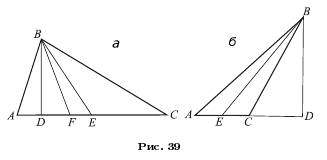
\includegraphics{mppics/ris-39}
\caption{}\label{1938/ris-39}
\end{figure}

Из вершины каждого угла треугольника можно опустить перпендикуляр на противоположную сторону или её продолжение;
следовательно, каждый треугольник имеет три высоты.
Вершину каждого угла треугольника можно соединить прямой с серединой противоположной стороны, следовательно, каждый треугольник имеет три медианы.
Точно так же ясно, что каждый треугольник имеет три биссектрисы.

\subsection*{Симметрия геометрических фигур относительно оси}



\begin{wrapfigure}{R}{48mm}
\centering
\includegraphics{mppics/ris-40}
\caption{}\label{1938/ris-40}
\end{wrapfigure}

\paragraph{}\label{1938/37}
При изучении свойств треугольников, многоугольников и других геометрических фигур часто встречается случай особого расположения на плоскости двух равных фигур или двух равных отрезков, или двух точек по отношению к какой-либо прямой.
Если какие-нибудь две точки $A$ и $A'$ (рис.~\ref{1938/ris-40}) расположены по разные стороны от прямой $MN$ на одном и том же перпендикуляре к этой прямой и на одинаковом расстоянии от основания перпендикуляра ($Aa=A'a$), то такие точки называются \index{симметрия относительно прямой}\textbf{симметричными} относительно прямой $MN$.

Две фигуры (или две части одной и той же фигуры) называются симметричными относительно прямой $MN$, если каждой точке $A$, $B$, $C$, $D$, $E,\dots$
(рис.~\ref{1938/ris-40}) одной фигуры (или одной части фигуры) соответствуют симметричные точки $A'$, $B'$, $C'$, $D'$, $E',\dots$ другой фигуры (или другой части фигуры), и обратно.
Прямая $MN$ в таком случае называется \index{ось симметрии}\textbf{осью симметрии}. 
Здесь слово «ось» применяется потому, что если часть плоскости, лежащую по одну сторону от прямой $MN$ (например, левую часть), станем вращать вокруг $MN$, как около оси, до тех пор, пока эта часть плоскости не упадёт на ту часть, которая лежит по другую сторону от прямой $MN$ (на правую часть), то симметричные фигуры совместятся, так как точка $A$ упадёт при этом в точку $A'$, точка $B$ — в точку $B'$ и~т.~д.

Обратно, если вращением вокруг некоторой прямой мы можем фигуру, лежащую по одну сторону от этой прямой, совместить с фигурой, лежащей по другую её сторону, то эти фигуры симметричны относительно оси вращения.
Из сказанного следует, что.

\textbf{\emph{всякие две фигуры, симметричные относительно какой-либо оси, равны между собой.}}

Симметрия относительно оси называется \index{осевая симметрия}\textbf{осевой симметрией}. 

\smallskip
\so{Замечание}.
Хотя симметричные фигуры вращением вокруг оси симметрии могут быть приведены в совмещение, однако они, вообще говоря, не тождественны в своём расположении на плоскости.
Это нужно понимать в следующем смысле.

чтобы совместить две симметричные фигуры, необходимо одну из них перевернуть другой стороной и, следовательно, на время вывести её из плоскости.
Если же не выводить фигуры из плоскости, то, вообще говоря, никаким перемещением в этой плоскости нельзя привести её к совпадению с фигурой, ей симметричной относительно оси.

\begin{wrapfigure}{l}{36mm}
\centering
\includegraphics{mppics/ris-41}
\caption{}\label{1938/ris-41}
\end{wrapfigure}

На рис.~\ref{1938/ris-41} изображены два узора, симметричные относительно прямой $AB$.
Вращая правый узор около прямой $AB$, его можно совместить с левым узором.

При этом правый узор будет перевёрнут другой стороной.
Но если не отрывать правого узора от плоскости, а перемещать его так, чтобы он скользил по плоскости, то никаким передвижением его не удастся совместить с левым узором.

Осевая симметрия часто встречается в обыденной жизни.
Узоры на декоративных тканях и на комнатных обоях, архитектурные украшения на зданиях в виде плоских рисунков и самые фасады зданий имеют обычно форму, симметричную относительно некоторой оси.
В природе также часто встречаются симметричные формы.
Так, листья деревьев и лепестки цветов имеют форму, симметричную относительно среднего стебля.
Таков изображённый на рис.~\ref{1938/ris-42} лист клёна.
Крылья бабочки и их расцветка имеют форму, симметричную относительно оси её туловища (рис.~\ref{1938/ris-43}).

\begin{figure}[h!]
\begin{minipage}{.48\textwidth}
\centering
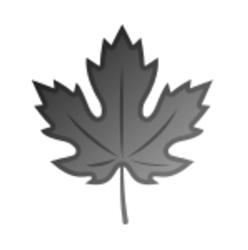
\includegraphics{eps/klenovyj-list}
\caption{}\label{1938/ris-42}
\end{minipage}\hfill
\begin{minipage}{.48\textwidth}
\centering

\includegraphics{eps/babochka}
\caption{}\label{1938/ris-43}
\end{minipage}
\end{figure}

\subsection*{Некоторые свойства равнобедренного треугольника}

\paragraph{}\label{1938/38}
\so{Теоремы}.
1) \textbf{\emph{В равнобедренном треугольнике биссектриса угла при вершине есть одновременно и медиана и высота.}}

2) \textbf{\emph{В равнобедренном треугольнике углы при основании равны.}}

\begin{wrapfigure}{R}{36mm}
\centering
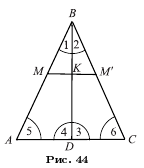
\includegraphics{mppics/ris-44}
\caption{}\label{1938/ris-44}
\end{wrapfigure}


Пусть $\triangle ABC$ (рис.~\ref{1938/ris-44}) равнобедренный и прямая $BD$ делит пополам угол $B$ при вершине его.
Требуется доказать, что эта биссектриса $BD$ есть также и медиана и высота.

Вообразим, что $\triangle ABD$ повёрнут вокруг стороны $BD$, как около оси, так, чтобы он упал на $\triangle BDC$.
Тогда, вследствие равенства углов 1 и 2, сторона $AB$ упадёт на $BC$, а вследствие равенства этих сторон точка $A$ совпадёт с $C$.
Поэтому $BA$ совместится с $BC$, угол 4 совместится с углом 3 и угол 5 — с углом 6;
значит,
\[DA = BC,\quad \angle 4 = \angle 3\quad \text{и}\quad \angle 5 = \angle 6.\]

Из того, что $DA=DC$, следует, что $BD$ есть медиана;
из того, что углы 3 и 4 равны, вытекает, что эти углы прямые и, следовательно, $BD$ есть высота треугольника, и, наконец, углы 5 и 6 при основании треугольника равны.

\paragraph{}\label{1938/39}
\so{Следствие}.
Мы видим, что в равнобедренном треугольнике $ABC$ (рис.~\ref{1938/ris-44}) одна и та же прямая $BD$ обладает четырьмя свойствами:
она есть биссектриса угла при вершине, медиана, проведённая к основанию, высота, опущенная на основание, и, наконец, перпендикуляр к основанию, восстановленный из его середины. 
Перпендикуляр к отрезку, восстановленный из его середины называется \index{срединный перпендикуляр}\textbf{срединным перпендикуляром} к этому отрезку.

Так как каждое из этих четырёх свойств вполне определяет положение прямой $BD$, то существование одного из них влечёт за собой все остальные.
Например, \emph{высота, опущенная на основание равнобедренного треугольника, служит одновременно биссектрисой угла при вершине, медианой, проведённой к основанию, и срединным перпендикуляром к основанию.} 

\paragraph{Симметрия равнобедренного треугольника.}\label{1938/40}
Мы видели, что равнобедренный $\triangle ABC$ (рис.~\ref{1938/ris-44}) делится биссектрисой $BD$ на такие два треугольника (левый и правый), которые вращением вокруг биссектрисы могут быть совмещены один с другим.
Из этого можно заключить, что какую бы точку на одной половине равнобедренного треугольника мы ни взяли, всегда можно на другой его половине найти точку, симметричную с первой относительно оси $BD$.
Возьмём, например, на стороне $AB$ точку $M$ (рис.~\ref{1938/ris-44}).
Опустим из неё на $BD$ перпендикуляр $MK$ и продолжим его до пересечения со стороной $BC$.
Мы получим тогда на этой стороне точку $M'$, симметричную с точкой $M$ относительно оси $BD$.
Действительно, если, вращая $\triangle ABD$ вокруг $BD$, мы его совместим с $\triangle BCD$, то при этом $KM$ пойдёт по $KM'$ (по равенству прямых углов), а сторона $BA$ упадёт на сторону $BC$ (по равенству углов при вершине $B$);
значит, точка $M$, которая лежит на $KM$ и на $BA$, упадёт в точку $M'$, которая лежит и на $KM'$, и на $BC$.
Отсюда видно, что $KM=KM'$.
Таким образом, точки $M$ и $M'$ лежат по разные стороны от биссектрисы $BD$, на одном к ней перпендикуляре и на равных расстояниях от основания этого перпендикуляра;
значит, эти точки симметричны относительно оси $BD$.
Таким образом, \emph{в равнобедренном треугольнике биссектриса угла при вершине есть его ось симметрии.}

\subsection*{Признаки равенства треугольников}

\paragraph{Предварительные понятия.}\label{1938/41}
Две геометрические фигуры, например два треугольника, как мы знаем, называются равными, если они при наложении могут быть совмещены.
В совмещающихся треугольниках, конечно, должны быть соответственно равны все элементы их, то есть стороны, углы, высоты, медианы и биссектрисы.
Однако для того, чтобы утверждать, что два треугольника равны, нет необходимости устанавливать равенства всех их элементов, достаточно убедиться в равенстве только некоторых из них.

\paragraph{Три признака равенства треугольников.}\label{1938/42}
\so{Теоремы}.
1) \textbf{\emph{Если две стороны и угол, заключённый
между ними, одного треугольника соответственно равны
двум сторонам и углу, заключённому между ними, другого треугольника, то такие треугольники равны.}}

2) \textbf{\emph{Если два угла и прилежащая к ним сторона одного треугольника соответственно равны двум углам и прилежащей к ним стороне другого треугольника, то такие треугольники равны.}}

3) \textbf{\emph{Если три стороны одного треугольника равны трём сторонам другого треугольника, то такие треугольники равны.}}

1) Пусть $ABC$ и $A_1B_1C_1$ — два треугольника (рис.~\ref{1938/ris-45}), у которых
\[AC=A_1C_1,\quad AB = A_1B_1,\quad \angle A = \angle A_1.\]
Требуется доказать, что эти треугольники равны.

\begin{wrapfigure}{r}{50mm}
\centering
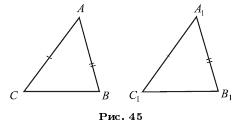
\includegraphics{mppics/ris-45}
\caption{}\label{1938/ris-45}
\end{wrapfigure}

Наложим $\triangle ABC$ на $\triangle A_1B_1C_1$ так, чтобы точка $A$ совпала с $A_1$ и сторона $AC$ пошла по $A_1C_1$%
\footnote{Для выполнения указанных в этом параграфе наложений иногда приходится накладываемый треугольник перевернуть другой стороной.}%
.
Тогда, вследствие равенства этих сторон, точка $C$ совместится с $C_1$, вследствие равенства углов $A$ и $A_1$ сторона $AB$ пойдёт по $A_1B_1$, а вследствие равенства этих сторон точка $B$ совпадёт с $B_1$, поэтому сторона $CB$ совместится с $C_1B_1$ (так как две точки можно соединить только одной прямой), и треугольники совпадут;
значит, они равны.


2) Пусть $ABC$ и $A_1B_1C_1$ (рис.~\ref{1938/ris-46}) — два треугольника, у которых
\[\angle C= \angle C_1,
\quad
\angle B=\angle B_1,
\quad
CB = C_1B_1.\]
Требуется доказать, что эти треугольники равны.

\begin{wrapfigure}{r}{50mm}
\centering
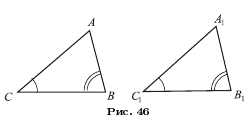
\includegraphics{mppics/ris-46}
\caption{}\label{1938/ris-46}
\end{wrapfigure}

Наложим $\triangle ABC$ на $\triangle A_1B_1C_1$ так, чтобы точка $C$ совпала с $C_1$ и сторона $CB$ пошла по $C_1B_1$.
Тогда, вследствие равенства этих сторон, точка $B$ совпадёт с $B_1$, а вследствие равенства углов $B$ и $B_1$, $C$ и $C_1$, сторона $BA$ пойдёт по $B_1A_1$ и сторона $CA$ — по $C_1A_1$.

Так как две прямые могут пересечься только в одной точке, то вершина $A$ должна совпасть с $A_1$.
Таким образом, треугольники совместятся;
значит, они равны.

3) Пусть $ABC$ и $A_1B_1C_1$ (рис.~\ref{1938/ris-47}) — два треугольника, у которых
\[AB = A_1B_1,
\quad
BC = B_1C_1,\quad 
CA = C_1A_1.
\]
Требуется доказать, что эти треугольники равны.

Доказывать этот признак равенства наложением, как мы это делали для первых признаков, было бы неудобно, так как, не зная ничего о величине углов, мы не можем утверждать, что при совпадении двух равных сторон совпадут и остальные стороны.
Вместо наложения применим здесь \textbf{приложение}.

Приложим $\triangle ABC$ к $\triangle A_1B_1C_1$ так, чтобы у них совместились равные стороны $AC$ и $A_1C_1$.
Тогда $\triangle ABC$ займёт положение $\triangle A_1C_1B_2$.

\begin{wrapfigure}{r}{40mm}
\centering
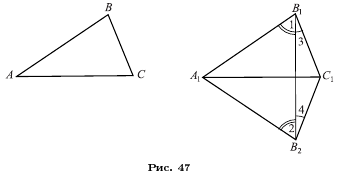
\includegraphics{mppics/ris-47}
\caption{}\label{1938/ris-47}
\end{wrapfigure}

Соединив прямой точки $B_1$ и $B_2$, мы получим два равнобедренных треугольника $A_1B_1B_2$ и $B_1C_1B_2$ с общим основанием $B_1B_2$.
Но в равнобедренном треугольнике углы при основании равны (§~\ref{1938/38});
следовательно, $\angle 1 = \angle 2$ и $\angle 3 = \angle 4$, а потому $\angle A_1B_1C_1 = \angle A_1B_2C_1 = \angle B$.
Но в таком случае данные треугольники должны быть равны, так как две стороны и угол, заключённый между ними, одного треугольника соответственно равны двум сторонам и углу, заключённому между ними, другого треугольника.
%\footnote{Чтобы прямая $B_1B_2$ проходила всегда внутри фигуры $A_1B_1C_1B_2$, надо прикладывать треугольники друг к другу так, чтобы их общая сторона $A_1C_1$ была наибольшей из сторон.}%здесь был небольшой обман — я вернул вариант из 43(1914).


Может случиться, что прямая $B_1B_2$ не пересечётся со стороной $A_1C_1$,
а пойдёт вне треугольников (если сумма углов $C$ и $C_1$, большее $180\degree$),
или сольётся с линией $B_1C_1B_2$ (если $\angle C +\angle  C_1 = 180\degree$). Доказательство остаётся то же самое, с той разницей, что углы $B_1$ и $B_2$
будут равны друг другу, не как \so{суммы} равных углов, а как их разности, (рис.~\ref{1914/ris-40}), или как углы при основании равнобедренного треугольника (рис.~\ref{1914/ris-41}).

\begin{figure}[h!]
\begin{minipage}{.48\textwidth}
\centering
\includegraphics{mppics/ris-471}
\caption{}\label{1914/ris-40}
\end{minipage}\hfill
\begin{minipage}{.48\textwidth}
\centering
\includegraphics{mppics/ris-472}
\caption{}\label{1914/ris-41}
\end{minipage}
\end{figure}


\smallskip
\mbox{\so{Замечание}.}
\emph{В равных треугольниках против равных сторон лежат равные углы, и обратно, против равных углов лежат равные стороны.}

Доказанные теоремы о равенстве треугольников и умение распознавать равные треугольники по указанным признакам чрезвычайно облегчают решение многих геометрических задач и необходимы для доказательства многих теорем.
Теоремы о равенстве треугольников являются главным средством для обнаружения свойств сложных геометрических фигур.
Учащиеся убедятся в этом при дальнейшем прохождении предмета.

\subsection*{Внешний угол треугольника и его свойства}

\paragraph{}\label{1938/43}
\mbox{\so{Определение}.}
Угол, смежный с каким-нибудь углом треугольника (или многоугольника), называется \index{внешний угол}\textbf{внешним} углом этого треугольника (или многоугольника). 

Таковы, например, углы $BCD$, $CBE$, $BAF$ (рис.~\ref{1938/ris-48}).
В отличие от внешних углы самого треугольника (или многоугольника) называются \index{внутренний угол}\textbf{внутренними}. 

При каждом угле треугольника (или многоугольника) можно построить по два внешних угла (продолжив одну или другую сторону угла).
Эти два угла равны, как углы вертикальные.

\begin{figure}[h!]
\begin{minipage}{.48\textwidth}
\centering
\includegraphics{mppics/ris-48}
\caption{}\label{1938/ris-48}
\end{minipage}\hfill
\begin{minipage}{.48\textwidth}
\centering
\includegraphics{mppics/ris-49}
\caption{}\label{1938/ris-49}
\end{minipage}
\end{figure}

\paragraph{}\label{1938/44}
\mbox{\so{Теорема}.}
\textbf{\emph{Внешний угол треугольника больше каждого внутреннего угла его, не смежного с этим внешним.}}


Например, докажем, что внешний угол $BCD$ треугольника $ABC$
(рис.~\ref{1938/ris-49}) больше каждого из внутренних углов $A$ и $B$, не смежных с этим внешним.

Через середину $E$ стороны $BC$ проведём медиану $AE$ и на её продолжении отложим отрезок $EF=AE$.
Точка $E$, очевидно, будет лежать внутри угла $BCD$.
Соединим $E$ с $C$ прямой.
Треугольники $ABE$ и $EFC$ (покрытые штрихами) равны, так как при точке $E$ они имеют по равному углу, заключённому между двумя соответственно равными сторонами.
Из равенства их заключаем, что углы $B$ и $ECF$, лежащие против равных сторон $AE$ и $EF$, равны.
Но угол $ECF$ составляет часть внешнего угла $BCD$ и потому меньше его;
следовательно, и угол $B$ меньше угла $BCD$.

{

\begin{wrapfigure}{r}{28mm}
\centering
\includegraphics{mppics/ris-50}
\caption{}\label{1938/ris-50}
\centering
\includegraphics{mppics/ris-51}
\caption{}\label{1938/ris-51}
\end{wrapfigure}

Продолжив сторону $BC$ за точку $C$, мы получим внешний угол $ACH$, равный углу $BCD$.
Если из вершины $B$ проведём к стороне $AC$ медиану и продолжим её на такую же длину за сторону $AC$, то совершенно так же докажем, что угол $A$ меньше угла $ACH$, то есть меньше угла $BCD$.

\paragraph{}\label{1938/45}
\mbox{\so{Следствие}.}
\emph{Если в треугольнике один угол прямой или тупой, то два других угла острые.}
Действительно, допустим, что угол $C$ треугольника $ABC$ 
(рис.~\ref{1938/ris-50} и \ref{1938/ris-51}) будет прямой или тупой, тогда смежный с ним внешний угол $BCD$ должен быть прямой или острый;
следовательно, углы $A$ и $B$, которые, по доказанному, меньше этого внешнего угла, должны быть оба острые.

}

\subsection*{Стороны и углы треугольника}

\paragraph{}\label{1938/46}
\so{Теоремы}.
Во всяком треугольнике

1) против равных сторон лежат равные углы.

2) против б\'{о}льшей стороны лежит больший угол.

1) Если две стороны треугольника равны, то он равнобедренный, тогда углы, лежащие против этих сторон, должны быть равны, как углы при основании равнобедренного треугольника (§~\ref{1938/38}).

2) Пусть в $\triangle ABC$ (рис.~\ref{1938/ris-52}) сторона $AB$ больше $BC$;
требуется доказать, что угол $C$ больше угла $A$.

\begin{wrapfigure}{r}{33mm}
\centering
\includegraphics{mppics/ris-52}
\caption{}\label{1938/ris-52}
\end{wrapfigure}

Отложим на б\'{о}льшей стороне $BA$ от вершины $B$ отрезок $BD$, равный меньшей стороне $BC$, и соединим $D$ с $C$ прямой.
Тогда получим равнобедренный $\triangle BDC$, у которого углы при основании равны, то есть $\angle BDC=\angle BCD$.
Но угол $BDC$ как внешний по отношению к $\angle ADC$, больше угла $A$, следовательно, и угол $BCD$ больше угла $A$, а потому и подавно угол $BCA$ больше угла $A$, что и требовалось доказать.

\paragraph{}\label{1938/47}
\so{Обратные теоремы}.
\textbf{\emph{Во всяком треугольнике.}}

1) \textbf{\emph{против равных углов лежат равные стороны;}}

2) \textbf{\emph{против б\'{о}льшего угла лежит б\'{о}льшая сторона.}}

\begin{wrapfigure}{R}{32mm}
\centering
\includegraphics{mppics/ris-53}
\caption{}\label{1938/ris-53}
\bigskip
\includegraphics{mppics/ris-54}
\caption{}\label{1938/ris-54}
\end{wrapfigure}

1) Пусть в $\triangle ABC$ углы $A$ и $C$ равны (рис.~\ref{1938/ris-53});
требуется доказать, что $BA = BC$.

Предположим противное, то есть что стороны $AB$ и $BC$ не равны.
Тогда одна из этих сторон должна быть больше другой, и, следовательно, согласно прямой теореме, один из углов $A$ и $C$ должен быть больше другого.
Но это противоречит условию, что $\angle A = \angle C$;
значит, нельзя допустить, что стороны $AB$ и $BC$ не равны;
остаётся принять, что $AB=BC$.

2) Пусть в $\triangle ABC$ (рис.~\ref{1938/ris-54})
угол $C$ больше угла $A$;
требуется доказать, что $AB > BC$.

Предположим противное, то есть что $AB$ не больше $BC$.
Тогда могут представиться два случая:
или $AB=BC$, или $AB<BC$.

В первом случае, согласно прямой теореме, угол $C$ был бы равен углу $A$, во втором случае угол $C$ был бы меньше угла $A$;
и то и другое противоречит условию;
значит, оба эти случая исключаются.
Остаётся один возможный случай, что $AB>BC$.

\smallskip
\mbox{\so{Следствия}.}
1) \emph{В равностороннем треугольнике все углы равны.}

2) \emph{В равноугольном треугольнике все стороны равны.}

\paragraph{Доказательство от противного.}\label{1938/48}
Способ, которым мы только что доказали обратные теоремы, называется \index{доказательство от противного}\textbf{доказательством от противного}, или приведением к \index{противоречие}\textbf{противоречию}.
Первое название этот способ получил потому, что в начале рассуждения делается предположение, противное (противоположное) тому, что требуется доказать.
Приведением к противоречию он называется вследствие того, что, рассуждая на основании сделанного предположения, мы приходим к противоречию (к абсурду).
Получение такого вывода заставляет нас отвергнуть сделанное вначале допущение и принять то, которое требовалось доказать.

Этот приём очень часто употребляется для доказательства теорем.

\paragraph{Замечание об обратных теоремах.}\label{1938/49}
Начинающие изучать геометрию часто делают одну характерную ошибку.
Она заключается в том, что правильность обратной теоремы считают само собой разумеющейся, если доказана прямая теорема.
Отсюда представление, что доказательство обратных теорем вообще излишне.
Ошибочность такого заключения может быть показана в ряде примеров.
В частности, такой пример был приведён в §~\ref{1938/30}.
Поэтому обратные теоремы, когда они верны, всегда доказываются особо.



\subsection*{Длина ломаной.}

\paragraph{}\label{1938/50}
\so{Теорема}.
\textbf{\emph{В треугольнике каждая сторона меньше суммы двух других сторон.}}

Если в треугольнике возьмём сторону не самую большую, то, конечно, она окажется менее суммы двух других сторон.
Значит, нам надо доказать, что даже \so{наибольшая} сторона треугольника меньше суммы двух других сторон.

\begin{wrapfigure}{R}{32mm}
\centering
\includegraphics{mppics/ris-55}
\caption{}\label{1938/ris-55}
\end{wrapfigure}

Пусть в $\triangle ABC$ (рис.~\ref{1938/ris-55}) наибольшая сторона есть $AC$.
Продолжив сторону $AB$, отложим $BD=BC$ и проведём $DC$.
Так как $\triangle BDC$ равнобедренный, то $\angle D = \angle DCB$;
поэтому угол $D$ меньше угла $DCA$, и, следовательно, в $\triangle ADC$ сторона $AC$ меньше $AD$ (§~\ref{1938/47}), то есть
$AC < AB + BD$.
Заменив $BD$ на $BC$, получим:
\[AC < AB + BC.\]
\smallskip
\so{Следствие}.
Отнимем от обеих частей выведенного неравенства по $AB$ или по $BC$.
\begin{align*}
AC-AB&<BC;
\\
AC-BC&<AB.
\end{align*}
Читая эти неравенства справа налево, видим, что каждая из сторон $BC$ и $AB$ больше разности двух других сторон;
так как это же можно, очевидно, сказать и о третьей, наибольшей стороне $AC$, то, значит, \emph{в треугольнике каждая сторона больше разности двух других сторон.}

\begin{wrapfigure}{r}{32mm}
\centering
\includegraphics{mppics/ris-56}
\caption{}\label{1938/ris-56}
\end{wrapfigure}

\paragraph{}\label{1938/51}
\mbox{\so{Теорема}.}
\textbf{\emph{Отрезок, соединяющий две какие-нибудь точки, меньше всякой ломаной, соединяющей эти же точки.}}

Если ломаная, о которой говорится здесь, состоит только из двух сторон, то теорема уже была доказана в предыдущем параграфе.
Рассмотрим случай, когда ломаная состоит более чем из двух сторон.
Пусть $AE$ (рис.~\ref{1938/ris-56}) есть отрезок, соединяющий точки $A$ и $E$, а $ABCDE$ — какая-нибудь ломаная, соединяющая те же точки.
Требуется доказать, что $AE$ меньше суммы $AB+BC+CD+DE$.
Соединив $A$ с $C$ и $D$, находим, согласно предыдущей теореме.
\begin{align*}
AE&<AD+DE;
\\
AD&<AC +CD;
\\
AC&<AB+BC.
\end{align*}

Сложим почленно эти неравенства и затем от обеих частей полученного неравенства отнимем по $AD$ и $AC$, тогда получим:
\[AE<AB+BC +CD + DE.\]

\paragraph{Треугольники с двумя соответственно равными сторонами.}\label{1938/52}\ 
\smallskip
\so{Теоремы}.
\textbf{\emph{Если две стороны одного треугольника соответственно равны двум сторонам другого треугольника, то:}}

1) \textbf{\emph{против большего из углов, заключённых между ними, лежит б\'{о}льшая сторона.}}

2) \so{обратно}:
\textbf{\emph{против б\'{о}льшей из неравных сторон лежит больший угол.}}

\begin{figure}[h!]
\centering
\includegraphics{mppics/ris-57}
\caption{}\label{1938/ris-57}
\end{figure}

1) Пусть в треугольниках $ABC$ и $A_1B_1C_1$ дано (рис.~\ref{1938/ris-57}):
$AC\z=A_1C_1$, $AB=A_1B_1$ и $\angle A > \angle A_1$.
Требуется доказать, что $BC\z>B_1C_1$.
Наложим $\triangle A_1B_1C_1$ на $\triangle ABC$ так, чтобы сторона $A_1C_1$ совпадала с $AC$.
Так как $\angle A_1 < \angle BAC$, то сторона $A_1B_1$ пойдёт внутри угла $BAC$;
пусть $\triangle A_1B_1C_1$ займёт положение $AB_2C$ (вершина $B_2$ может оказаться или вне $\triangle ABC$, или внутри него, или же на стороне $BC$;
доказательство может быть применено ко всем этим случаям).
Проведём биссектрису $AD$ угла $BAB_2$ и соединим $D$ с $B_2$;
тогда получим два треугольника:
$ABD$ и $DAB_2$, которые равны, потому что у них $AB$ — общая сторона, $AB=AB_2$ по условию и $\angle BAD=\angle DAB_2$ по построению.
Из равенства треугольников следует:
$BD=DB_2$.
Из $\triangle DCB_2$ выводим:
$B_2C < B_2D + DC$ (§~\ref{1938/50}), или (заменив $B_2D$ на $BD$):
\[B_2C <BD +DC,\quad\text{значит,}\quad B_1C_1 < BC.\]

2) Пусть в тех же треугольниках $ABC$ и $A_1B_1C_1$ дано:
$AB\z=A_1B_1$;
$AC=A_1C_1$ и $BC>B_1C_1$;
докажем, что $\angle A > \angle A_1$.

Допустим противное, то есть что угол $A$ не больше угла $A_1$, тогда могут представиться два случая:
или $\angle BAC = \angle A_1$, или $\angle BAC \z< \angle A_1$.
В первом случае треугольники были бы равны и, следовательно, сторона $BC$ равнялась бы $B_1C_1$, что противоречит условию;
во втором случае сторона $BC$ (согласно теореме 1) была бы меньше $B_1C_1$, что также противоречит условию.
Значит, оба эти случая исключаются;
остаётся один возможный случай, что $\angle A > \angle A_1$.


\subsection*{Сравнительная длина перпендикуляра и наклонных}

{\sloppy

\paragraph{}\label{1938/53}
\so{Теорема}.
\textbf{\emph{Перпендикуляр, опущенный из какой-нибудь точки на прямую, меньше всякой наклонной, проведённой из той же точки на эту прямую%
\footnote{В §§~\ref{1938/53}, \ref{1938/54} и \ref{1938/55} ради краткости термины «перпендикуляр» и «наклонная» употребляются вместо «отрезок перпендикуляра, ограниченный данной точкой и основанием перпендикуляра» и «отрезок наклонной, ограниченный данной точкой и основанием наклонной».}.%
}}

}

\begin{wrapfigure}{R}{32mm}
\centering
\includegraphics{mppics/ris-58}
\caption{}\label{1938/ris-58}
\end{wrapfigure}

Пусть $AB$ (рис.~\ref{1938/ris-58}) есть перпендикуляр, опущенный из точки $A$ на прямую $MN$, и $AC$ — какая-нибудь наклонная, проведённая из той же точки $A$ к прямой $MN$;
требуется доказать, что $AB<AC$.

В $\triangle ABC$ угол $B$ прямой, а угол $C$ острый (§~\ref{1938/45});
значит, $\angle C<\angle B$ и потому $AB<AC$, что и требовалось доказать.

\smallskip
\mbox{\so{Замечание}.}
Когда говорят:
«расстояние от точки до прямой», имеется в виду \so{кратчайшее} расстояние, измеряемое по перпендикуляру, опущенному из этой точки на прямую.

\paragraph{}\label{1938/54}
\so{Теорема}.
\textbf{\emph{Если из одной и той же точки, взятой вне прямой, проведены к этой прямой перпендикуляр и какие-нибудь наклонные, то:}}

1) \textbf{\emph{если основания двух наклонных одинаково удалены от основания перпендикуляра, то такие наклонные равны.}}

2) \textbf{\emph{если основания двух наклонных неодинаково удалены от основания перпендикуляра, то та из наклонных больше, основание которой дальше отстоит от основания перпендикуляра.}}

\begin{wrapfigure}{R}{42mm}
\centering
\includegraphics{mppics/ris-59}
\caption{}\label{1938/ris-59}
\end{wrapfigure}

1) Пусть $AC$ и $AD$ (рис.~\ref{1938/ris-59}) будут две наклонные, проведённые из точки $A$ к прямой $MN$, основания которых $C$ и $D$ одинаково удалены от основания перпендикуляра $AB$, то есть $CB\z=BD$;
требуется доказать, что $AC = AD$.

В треугольниках $ABC$ и $ABD$ есть общая сторона $AB$ и сверх того $BC\z=BD$ (по условию) и $\angle ABC \z= \angle ABD$ (как углы прямые);
значит, эти треугольники равны, и потому $AC = AD$.

2) Пусть $AC$ и $AE$ (рис.~\ref{1938/ris-59}) будут две такие наклонные, проведённые из точки $A$ к прямой $MN$, основания которых неодинаково удалены от основания перпендикуляра;
например, пусть $BE>BC$.
Требуется доказать, что $AE>AC$.

Отложим $BD=BC$ и проведём $AD$.
По доказанному выше $AE \z= AC$.
Сравним $AE$ с $AD$.
Угол $ADE$ есть внешний по отношению $\triangle ABD$, и потому он больше прямого угла $ABD$;
следовательно, угол $ADE$ тупой, и потому угол $AED$ должен быть острый (§~\ref{1938/45}), значит, $\angle ADE>\angle AED$ и, следовательно, $AE>AD$, и потому $AE>AC$.

\paragraph{}\label{1938/55}
\so{Обратные теоремы}.
\textbf{\emph{Если из одной и той же точки, взятой вне прямой}} (рис.~\ref{1938/ris-59}), \textbf{\emph{проведены к этой прямой перпендикуляр и какие-нибудь наклонные, то:}}

1) \textbf{\emph{если две наклонные равны, то их основания одинаково удалены от основания перпендикуляра.}}

2) \textbf{\emph{если две наклонные не равны, то основание б\'{о}льшей из них дальше отстоит от основания перпендикуляра.}}

Предоставляем учащимся самим доказать эти теоремы (способом от противного).

\subsection*{Признаки равенства прямоугольных треугольников}

\paragraph{Два признака, не требующие особого доказательства.}\label{1938/56}

Так как в прямоугольных треугольниках углы, содержащиеся между катетами, всегда равны, как углы прямые, то \textbf{\emph{прямоугольные треугольники равны.}}

1) \textbf{\emph{если катеты одного треугольника соответственно равны катетам другого;}}

2) \textbf{\emph{если катет и прилежащий к нему острый угол одного треугольника соответственно равны катету и прилежащему к нему острому углу другого треугольника.}}

Эти два признака не требуют особого доказательства, так как они представляют частные случаи общих признаков.
Докажем ещё два следующих признака, относящихся только к прямоугольным треугольникам.

\paragraph{Два признака, требующие особого доказательства.}\label{1938/57}
\so{Теоремы}.
\textbf{\emph{Прямоугольные треугольники равны:}}

1) \textbf{\emph{если гипотенуза и острый угол одного треугольника соответственно равны гипотенузе и острому углу другого}} или

2) \textbf{\emph{если гипотенуза и катет одного треугольника соответственно равны гипотенузе и катету другого.}}

\begin{figure}[h!]
\centering
\includegraphics{mppics/ris-60}
\caption{}\label{1938/ris-60}
\end{figure}

1) Пусть $ABC$ и $\triangle A_1B_1C_1$ (рис.~\ref{1938/ris-60}) — два прямоугольных треугольника, у которых $AB=A_1B_1$ и $\angle A = \angle A_1$;
требуется доказать, что эти треугольники равны.

Наложим $\triangle ABC$ на $\triangle A_1B_1C_1$ так, чтобы у них совместились равные гипотенузы.
Тогда по равенству углов $A$ и $A_1$ катет $AC$ пойдёт по $A_1C_1$.
При этом точка $C$ должна совпадать с точкой $C_1$, потому что если предположим, что она не совпадёт с точкой $C_1$, то тогда катет $BC$ занял бы положение $B_1C_2$ или $B_1C_3$, что невозможно, так как из одной точки $B_1$ нельзя на прямую $A_1C_1$ опустить два перпендикуляра ($B_1C_1$ и $B_1C_2$ или $B_1C_1$ и $B_1C_3$).

\begin{figure}[h!]
\begin{minipage}{.48\textwidth}
\centering
\includegraphics{mppics/ris-61}
\caption{}\label{1938/ris-61}
\end{minipage}\hfill
\begin{minipage}{.48\textwidth}
\centering
\includegraphics{mppics/ris-62}
\caption{}\label{1938/ris-62}
\end{minipage}
\end{figure}

2) Пусть (рис.~\ref{1938/ris-61} и \ref{1938/ris-62}) в прямоугольных треугольниках дано:
$AB=A_1B_1$ и $BC=B_1C_1$;
требуется доказать, что треугольники равны.
Наложим $\triangle ABC$ на $\triangle A_1B_1C_1$ так, чтобы у них совместились равные катеты $BC$ и $B_1C_1$.
Тогда по равенству прямых углов $CA$ пойдёт по $C_1A_1$.
При этом гипотенуза $AB$ не может не совместиться с гипотенузой $A_1B_1$, потому что, если бы она заняла положение $A_2B_1$ или $A_3B_1$, то тогда мы имели бы две равные наклонные ($A_1B_1$ и $A_2B_1$ или $A_1B_1$ и $A_3B_1$, которые неодинаково удалены от основания перпендикуляра, что невозможно (§~\ref{1938/54}).

\subsection*{Срединный перпендикуляр и биссектриса} 

\paragraph{}\label{1938/58}
Свойство срединного перпендикуляра к отрезку, и свойство биссектрисы угла очень сходны между собой.
Чтобы лучше видеть сходство этих свойств, мы изложим их параллельно.

\columnratio{0.5}
\setlength{\columnseprule}{.2pt}
\begin{paracol}{2}

{\sloppy

\textbf{\emph{1) Если какая-нибудь точка}} ($K$, рис.~\ref{1938/ris-63}) \textbf{\emph{лежит на срединном перпендикуляре}} ($MN$), \textbf{\emph{к отрезку}} ($AB$), \textbf{\emph{то она одинаково удалена от концов этого отрезка}} (то есть $KA=KB$).

{\centering
\includegraphics{mppics/ris-63}
\captionof{figure}{}
\label{1938/ris-63}
\addtocounter{figure}{1}
}

\medskip

Так как $MN\perp AB$ и $AO\z=OB$, то $AK$ и $KB$ суть наклонные к $AB$, основания которых одинаково удалены от основания перпендикуляра, значит $KA=KB$.

2) \so{Обратная теорема}.

\textbf{\emph{Если какая-нибудь точка}} ($K$, рис.~\ref{1938/ris-63}) \textbf{\emph{одинаково удалена от концов отрезка $AB$}} (то есть если $KA=KB$), \textbf{\emph{то она лежит на перпендикуляре, проведённом к отрезку $AB$ через его середину.}}

Проведём через $K$ прямую $MN\perp AB$;
тогда мы получим два прямоугольных треугольника $KAO$ и $KBO$, которые, имея общий катет $KO$ и равные гипотенузы, равны, а потому $AO=OB$.
Значит, прямая $MN$, проведённая нами через $K$ перпендикулярно к $AB$, делит отрезок $AB$ пополам.

}

\switchcolumn

{\sloppy

\textbf{\emph{1) Если какая-нибудь точка}} ($K$, рис.~\ref{1938/ris-64}) \textbf{\emph{лежит на биссектрисе}} ($OM$ угла $AOB$), \textbf{\emph{то она одинаково удалена от сторон этого угла}} (то есть перпендикуляры $KD$ и $KC$ равны).



{\centering
\addtocounter{figure}{1}
\includegraphics{mppics/ris-64}
\captionof{figure}{}
\label{1938/ris-64}
\addtocounter{figure}{1}
}

\medskip

Так как $OM$ делит угол пополам, то прямоугольные треугольники $OCK$ и $ODK$, имея общую гипотенузу и равные острые углы при вершине $O$, равны и потому $KC=KB$.

2) \so{Обратная теорема}.

\textbf{\emph{Если какая-нибудь точка}} ($K$, рис.~\ref{1938/ris-64}) \textbf{\emph{внутри угла одинаково удалена от его сторон}} (то есть если перпендикуляры $KC$ и $KD$ равны), \textbf{\emph{то она лежит на биссектрисе этого угла.}}

Через $O$ и $K$ проведём прямую $OM$.
Тогда получим два прямоугольных треугольника $OCK$ и $ODK$, которые, имея общую гипотенузу и равные катеты $CK$ и $DK$, равны, а потому равны и углы при вершине $O$.
Значит, прямая $OM$, проведённая через точку $K$, будет биссектрисой угла $AOB$.



}
\end{paracol}


\paragraph{}\label{1938/59}
\so{Следствие}.
Из двух доказанных теорем (прямой и обратной) можно вывести следующие \so{противоположные теоремы:}

\medskip

\begin{paracol}{2}
{\sloppy
\textbf{\emph{Если какая-нибудь точка не лежит на срединном перпендикуляре к отрезку, то она неодинаково удалена от концов этого отрезка.}}

\medskip

{\centering
\includegraphics{mppics/ris-1931-62}
\captionof{figure}{}
\label{1931/ris-62}
\addtocounter{figure}{1}
}

}

\switchcolumn

{\sloppy

\textbf{\emph{Если какая-нибудь точка внутри угла не лежит на его биссектрисе, то она неодинаково удалена от сторон этого угла.}}

\medskip

{\centering
\includegraphics{mppics/ris-1931-63}
\captionof{figure}{}
\label{1931/ris-63}
\addtocounter{figure}{1}
}

}

\end{paracol}
\setlength{\columnseprule}{0pt}

\medskip

Предоставляем самим учащимся доказать эти теоремы (способом от противного).

\paragraph{Геометрическое место.}\label{1938/60}
Геометрическим местом точек, обладающих некоторым свойством, называется такая линия (или поверхность в пространстве) или вообще такая совокупность точек, которая содержит в себе все точки, обладающие этим свойством, и не содержит ни одной точки, не обладающей им.

Например, геометрическое место точек, находящихся на данном расстоянии $r$ от данной точки $C$, есть окружность с центром в точке $C$ и радиусом $r$.
Из теорем предыдущих параграфов следует:

\emph{Геометрическое место точек, одинаково удалённых от двух данных точек, есть срединный перпендикуляр к отрезку соединяющего эти точки.} 

\emph{Геометрическое место точек внутри угла, одинаково удалённых от его сторон, есть биссектриса этого угла.}

\begin{wrapfigure}{r}{40mm}
\centering
\includegraphics{mppics/ris-extra-1}
\caption{}\label{extra/1}
\end{wrapfigure}

\smallskip
\mbox{\so{Упражнение}.} Докажите, что геометрическое место точек, одинаково удалённых от двух данных пресекающихся прямых, состоит из пары прямых, делящих пополам углы, образованные данными прямыми.

Такие пары прямых всегда перпендикулярны поскольку угол между такими прямыми составлен из половин смежных углов.

\section{Задачи на построение}

\paragraph{Предварительное замечание.}\label{1938/61}
Теоремы, доказанные нами ранее, позволяют решать некоторые задачи на \so{построение}.
Заметим, что в элементарной геометрии рассматриваются только такие построения, которые могут быть выполнены с помощью \so{линейки и циркуля}.
Употребление чертёжного треугольника и некоторых других приборов хотя и допускается ради сокращения времени, но не является необходимым.

\paragraph{}\label{1938/62}
\so{Задача 1}.
\emph{Построить треугольник по трём его сторонам $a$, $b$ и $c$} (рис.~\ref{1938/ris-65}).

\begin{figure}[h!]
\centering
\includegraphics{mppics/ris-65}
\caption{}\label{1938/ris-65}
\end{figure}

На какой-нибудь прямой $MN$ откладываем отрезок $CB$, равный одной из данных сторон, например $a$.
Описываем две небольшие дуги с центрами в точках $C$ и $B$, одну радиусом, равным $b$, другую радиусом, равным $c$.
Точку $A$, в которой эти дуги пересекаются, соединяем с $B$ и С;
$\triangle ABC$ будет искомый.

\smallskip
\so{Замечание}.
Чтобы три отрезка могли служить сторонами треугольника, необходимо и достаточно, чтобы больший из них был меньше суммы двух остальных (необходимость доказана в §~\ref{1938/50}, условие равносильное достаточности же будет принято за очевидное утверждение в \ref{1914/118}).

\paragraph{}\label{1938/63}
\so{Задача 2}.
\emph{Построить угол, равный данному углу $ABC$, одной из сторон которого является данная прямая и вершина которого находится в данной точке $O$} (точка $O$ расположена на прямой $MN$, рис.~\ref{1938/ris-66}).

\begin{figure}[h!]
\centering
\includegraphics{mppics/ris-66}
\caption{}\label{1938/ris-66}
\end{figure}

Описываем произвольным радиусом с центром в вершине $B$ между сторонами данного угла дугу $EF$;
затем, не изменяя раствора циркуля, переносим его остриё в точку $O$ и описываем дугу $PQ$.
Далее описываем дугу $ab$ с центром в точке $P$ радиусом, равным расстоянию между точками $E$ и $F$.
Наконец, через точки $O$ и $R$ (пересечение двух дуг) проводим прямую.
Угол $ROP$ равен углу $ABC$, потому что треугольники $ROP$ и $FBE$, имеющие соответственно равные стороны, равны.

\begin{wrapfigure}{r}{40mm}
\vskip-4mm
\centering
\includegraphics{mppics/ris-67}
\caption{}\label{1938/ris-67}
\bigskip
\includegraphics{mppics/ris-68}
\caption{}\label{1938/ris-68}
\end{wrapfigure}

\paragraph{}\label{1938/64}
\mbox{\so{Задача 3}.}
\emph{Разделить данный угол $ABC$ пополам (рис.~\ref{1938/ris-67}), другими словами, построить биссектрису данного угла или провести его ось симметрии.}
С центром в вершине $B$ произвольным радиусом опишем между сторонами угла дугу $DE$.
Затем, взяв произвольный раствор циркуля, больший, однако, половины расстояния между точками $E$ и $D$ (смотри замечание к задаче 1), описываем этим раствором небольшие дуги с центрами в точках $D$ и $E$, которые пересекутся в некоторой точке $F$.
Проведя прямую $BF$, мы получим биссектрису угла $ABC$.


Для доказательства соединим прямыми точку $F$ с $D$ и $E$;
тогда получим два треугольника $BEF$ и $BDF$, которые равны, так как у них $BP$ — общая сторона, $BD=BE$ и $DF=EF$ по построению.
Из равенства треугольников следует:
$\angle ABF = \angle CBF$.

\paragraph{}\label{1938/65}
\so{Задача 4}.
Из данной точки $C$ прямой $AB$ восстановить к этой прямой перпендикуляр (рис.~\ref{1938/ris-68}).

Отложим на $AB$ по обе стороны от данной точки $C$ равные отрезки (произвольной длины) $CD$ и $CE$.
С центрами в точках $E$ и $D$ одним и тем же раствором циркуля (б\'{о}льшим, однако, $CD$) опишем две небольшие дуги, которые пересекутся в некоторой точке $F$.
Прямая, проведённая через точки $C$ и $F$, будет искомым перпендикуляром.

Действительно, как видно из построения, точка $F$ одинаково удалена от точек $D$ и $E$;
следовательно, она должна лежать на срединном перпендикуляре к отрезку $DE$ (§~\ref{1938/58});
но середина этого отрезка есть $C$, а через точки $C$ и $F$ можно провести только одну прямую;
значит, $FC \perp DE$.

\paragraph{}\label{1938/66}
\so{Задача 5}.
\emph{Из данной точки $A$ опустить перпендикуляр на данную прямую $BC$} (рис.~\ref{1938/ris-69}).

\begin{wrapfigure}{R}{40mm}
\centering
\includegraphics{mppics/ris-69}
\caption{}\label{1938/ris-69}
\bigskip
\includegraphics{mppics/ris-70}
\caption{}\label{1938/ris-70}
\end{wrapfigure}

С центром в точке $A$ произвольным раствором циркуля (б\'{о}льшим, однако, расстояния от $A$ до $BC$) опишем дугу, которая пересечётся с $BC$ в каких-нибудь точках $D$ и $E$.
С центрами в этих точках произвольным, но одним и тем же раствором циркуля (б\'{о}льшим, однако, $\tfrac12\cdot DE$), проводим две небольшие дуги, которые пересекутся между собой в некоторой точке $F$.
Прямая $AF$ будет искомым перпендикуляром.

Действительно, как видно из построения, каждая из точек $A$ и $F$ одинаково удалена от $D$ и $E$, а такие точки лежат на срединном перпендикуляре к отрезку $DE$ (§~\ref{1938/58}).

\paragraph{}\label{1938/67}
\mbox{\so{Задача 6}.}
\emph{Провести срединный перпендикуляр к данному отрезку \emph{($AB$)}} (рис.~\ref{1938/ris-70}).

Произвольным, но одинаковым раствором циркуля (б\'{о}льшим $\tfrac12\cdot AB$) описываем две дуги с центрами в точках $A$ и $B$, которые пересекутся между собой в некоторых точках $C$ и $D$.
Прямая $CD$ будет искомым перпендикуляром.

Действительно, как видно из построения, каждая из точек $C$ и $D$ одинаково удалена от $A$ и $B$;
следовательно, эти точки должны лежать на оси симметрии отрезка $AB$.

\smallskip
\so{Задача 7}.
\emph{Разделить пополам данный отрезок} (рис.~\ref{1938/ris-70}).
Решается так же, как предыдущая задача.

\paragraph{Пример более сложной задачи.}\label{1938/68}
При помощи этих основных задач можно решать задачи более сложные.
Для примера решим следующую задачу.

\smallskip
\so{Задача}.
\emph{Построить треугольник, зная его основание $B$, угол $\alpha$, прилежащий к основанию, и сумму $s$ двух боковых сторон} (рис.~71).

\begin{figure}[h!]
\centering
\includegraphics{mppics/ris-71}
\caption{}\label{1938/ris-71}
\end{figure}

Чтобы составить план решения, предположим, что задача решена, то есть что найден такой $\triangle ABC'$, у которого основание $AC = b$, $\angle A=\alpha$ и $AB+BC=s$.
Рассмотрим полученный чертёж.
Сторону $AC$, равную $b$, и угол $A$, равный $\alpha$, мы построить умеем.
Значит, остаётся найти на другой стороне угла $A$ такую точку $B$, чтобы сумма $AB+BC$ равнялась $s$.
Продолжив $AB$, отложим отрезок $AD$, равный $s$.

Вопрос сводится к тому, чтобы на прямой $AB$ отыскать такую точку $B$, которая была бы одинаково удалена от $C$ и $B$.
Такая точка, как мы знаем (§~\ref{1938/58}), должна лежать на срединном перпендикуляре к отрезку $CD$. 
Точка $B$ найдётся в пересечении этого срединного перпендикуляра с $AD$. 

Итак, вот решение задачи:
строим (рис.~\ref{1938/ris-71}) угол $A$, равный данному углу $\alpha$;
на сторонах его откладываем $AC=b$ и $AD=s$ и соединяем точку $D$ с $C$.
Проведём срединный перпендикуляр к отрезку $CD$;
пересечение его с $AD$, то есть точку $B$, соединяем с $C$.
Треугольник $ABC$ будет  искомый, так как он удовлетворяет всем требованиям задачи:
у него $AC=b$, $\angle A = \alpha$ и $AB+BC=s$ (потому что $BD=BC$).

Рассматривая построение, мы замечаем, что задача возможна не при всяких данных.
Действительно, если сумма задана слишком малой сравнительно с $b$, то перпендикуляр $BE$ может не пересечь отрезка $AD$ (или пересечёт его продолжение за точку $A$ или за точку $D$);
в этом случае задача окажется невозможной.
И независимо от построения можно видеть, что задача невозможна, если $s<b$ или $s=b$, потому что не может быть такого треугольника, у которого сумма двух сторон была бы меньше или равна третьей стороне.

В том случае, когда задача возможна, она имеет только одно решение, то есть существует только один треугольник, удовлетворяющий требованиям задачи, так как перпендикуляр $BE$ может пересечься с прямой $AD$ только в одной точке.

\paragraph{}\label{1938/69}
\so{Замечание}.
Из приведённого примера видно, что решение сложной задачи на построение состоит из следующих четырёх частей.

1) Предположив, что задача решена, делают от руки приблизительный чертёж;
искомой фигуры и затем, внимательно рассматривая начерченную фигуру, стремятся найти такие зависимости между данными задачи и искомыми, которые позволили бы свести задачу к другим, известным ранее.
Эта самая важная часть решения задачи, имеющая целью составить план решения, носит название \textbf{анализа}.

2) Когда таким образом план решения найден, выполняют сообразно ему \textbf{построение}.

3) Для проверки правильности плана показывают затем на основании известных теорем, что полученная фигура удовлетворяет всем требованиям задачи.
Эта часть называется \textbf{синтезом}.

4) Затем задаются вопросом, при всяких ли данных задача возможна, допускает ли она одно решение или несколько, и нет ли в задаче каких-либо особенных случаев, когда построение упрощается или, наоборот, усложняется.
Эта часть решения называется \textbf{исследованием} задачи.

Когда задача очень проста и не может быть сомнения относительно её возможности, то обыкновенно анализ и исследование опускают, а указывают прямо построение и приводят доказательство.
Так мы делали, излагая решение первых семи задач этой главы;
так же будем делать и впоследствии, когда нам придётся излагать решения несложных задач.

\subsection*{Упражнения}

\begin{center}\so{Доказать теоремы}
\end{center}

\begin{enumerate}

 \item
В равнобедренном треугольнике две медианы равны, две биссектрисы равны, две высоты равны.

 \item
Если к каждой из равных сторон равнобедренного треугольника восстановим срединные перпендикуляры до пересечения с другой из равных сторон, то эти перпендикуляры будут равны. 

 \item
Прямая, перпендикулярная к биссектрисе угла, отсекает от его сторон равные отрезки.

 \item
Медиана треугольника меньше его полупериметра.

 \item
Медиана треугольника меньше полусуммы сторон, между которыми она заключается.

\smallskip
\so{Указание}.
Продолжить медиану на расстояние, равное ей, полученную точку соединить с одним концом стороны, к которой проведена медиана, и рассмотреть образовавшуюся фигуру.

 \item
Сумма медиан треугольника меньше периметра, но больше полупериметра.

\smallskip
\so{Указание}.
См. предыдущее упражнение, а также следствие в §~\ref{1938/50}.

 \item
Сумма диагоналей четырёхугольника меньше его периметра, но больше полупериметра.

 \item
Доказать как прямую теорему, что всякая точка, не лежащая на срединном перпендикуляре к отрезку, неодинаково удалена от концов этого отрезка, а именно: 
она ближе к тому концу, с которым она расположена по одну сторону от перпендикуляра.

 \item
Доказать как прямую теорему, что всякая точка, не лежащая на биссектрисе угла, неодинаково отстоит от сторон его.

 \item
Медиана, исходящая из какой-нибудь вершины треугольника, равно отстоит от двух других его вершин.

 \item
На одной стороне угла $A$ отложены отрезки $AB$ и $AC$ и на другой стороне отложены отрезки $AB'=AB$ и $AC' = AC$.
Доказать, что прямые $BC'$ и $B'C$ пересекаются на биссектрисе угла $A$.

 \item
Вывести отсюда способ построения биссектрисы угла.

 \item
Если $A'$ и $A$, $B'$ и $B$ — две пары точек, симметричных относительно какой-нибудь прямой $XY$, то четыре точки $A'$, $A$, $B'$, $B$ лежат на одной окружности.

 \item
Дан острый угол $XOY$ и точка $A$ внутри этого угла.
Найти на стороне $OX$ точку $B$ и на стороне $OY$ точку $C$ так, чтобы периметр $\triangle ABC$ был наименьший.

\smallskip
\so{Указание}.
Надо взять точки, симметричные с $A$ относительно сторон $OX$ и $OY$.

\end{enumerate}

\begin{center}
\so{Задачи на построение}
\end{center}

\begin{enumerate}[resume]

 \item
Построить сумму двух, трёх и более углов.

 \item
Построить разность двух углов.

 \item
По данной сумме и разности двух углов найти эти углы.

 \item
Разделить угол на 4, 8 и 16 равных частей.

 \item
Через вершину данного угла провести вне его такую прямую, которая со сторонами угла образовала бы равные углы.

 \item
Построить треугольник:
а) по двум сторонам и углу между ними;
б) по стороне и двум прилежащим углам;
в) по двум сторонам и углу, лежащему против б\'{о}льшей из них;
г) по двум сторонам и углу, лежащему против меньшей из них (в этом случае получаются два решения, или одно, или ни одного).

 \item
Построить равнобедренный треугольник:
а) по основанию и боковой стороне;
б) по основанию и прилежащему углу;
в) по боковой стороне и углу при вершине;
г) по боковой стороне и углу при основании.

 \item
Построить прямоугольный треугольник:
а) по двум катетам;
б) по катету и гипотенузе;
в) по катету и прилежащему острому углу.

 \item
Построить равнобедренный треугольник:
а) по высоте и боковой стороне;
б) по высоте и углу при вершине;
в) по основанию и перпендикуляру, опущенному из конца основания на боковую сторону.

 \item
Построить прямоугольный треугольник по гипотенузе и острому углу.

 \item
Через точку, данную внутри угла, провести такую прямую, которая отсекла бы от сторон угла равные части.

 \item
По данной сумме и разности двух отрезков найти эти отрезки.

 \item
Разделить данный отрезок на 4, 8, 16 равных частей.

 \item
На данной прямой найти точку, одинаково удалённую от двух данных точек (вне прямой).

 \item
Найти точку, равно отстоящую от трёх вершин треугольника.

 \item
На прямой, пересекающей стороны угла, найти точку, одинаково удалённую от сторон этого угла.

 \item
Найти точку, одинаково удалённую от трёх сторон треугольника.

 \item
На бесконечной прямой $AB$ найти такую точку $C$, чтобы полупрямые $CM$ и $CN$, проведённые из $C$ через данные точки $M$ и $N$, расположенные по одну сторону от $AB$, составляли с полупрямыми $CA$ и $CD$ равные углы.

\smallskip
\so{Указание}.
Построить точку $M'$, симметричную с $M$ относительно оси $AB$, и соединить $M'$ с $N$.

 \item
Построить прямоугольный треугольник по катету и сумме гипотенузы с другим катетом.

 \item
Построить треугольник по основанию, углу, прилежащему к основанию, и разности двух других сторон.
(Рассмотреть два случая:
1) когда дан меньший из двух углов, прилежащих к основанию;
2) когда дан больший из них.)

\smallskip
\so{Указание}.
См. задачу §~\ref{1938/68}.

 \item
Построить прямоугольный треугольник по катету и разности двух других сторон.

 \item
Дан угол $A$ и точки $B$ и $C$, расположенные одна на одной стороне угла, другая — на другой.
Найти:
1) точку $M$, равно отстоящую от сторон угла, и такую, чтобы $MC=MB$;
2) точку $N$, равно отстоящую от сторон угла так, чтобы $NC=CB$.

 \item
По соседству с железной дорогой расположены две деревни $A$ и $B$.
Найти на линии железной дороги (имеющей прямолинейную форму) место для станции, которая была бы одинаково удалена от $A$ и $B$.

 \item
Дан угол $A$ и точка $B$ на одной из его сторон.
Найти на другой стороне такую точку $C$, чтобы сумма $CA+CD$ была равна данному отрезку~$\ell$.

\end{enumerate}

\section{Параллельные прямые}

\subsection*{Основные теоремы}

\paragraph{}\label{1938/70}
\so{Определение}.
Две прямые называются \index{параллельные прямые}\textbf{параллельными}, если они лежат в одной плоскости и \textbf{не пересекаются}, сколько бы их ни продолжали.
При этом прямая также считается параллельной самой себе.

{

\begin{wrapfigure}{r}{25mm}
\centering
\includegraphics{mppics/ris-extra-3}
\caption{}\label{extra/ris-3}
\end{wrapfigure}

Параллельность прямых обозначается письменно знаком $\parallel$.
Так, если прямые $AB$ и $CD$ параллельны, то пишут:
$AB \parallel CD$. 
На чертежах параллельные прямые принято отмечать одинаковыми стрелочками как на рис. \ref{extra/ris-3}.

Возможность существования параллельных прямых обнаруживается следующей теоремой.

}

\paragraph{}\label{1938/71}
\mbox{\so{Теорема}.}
\textbf{\emph{Два перпендикуляра}} ($AB$ и $CD$, рис.~\ref{1938/ris-72}) \textbf{\emph{к одной и той же прямой}} ($MN$) \textbf{\emph{не могут пересечься, сколько бы мы их ни продолжали.}}

Действительно, если бы эти перпендикуляры пересеклись в какой-нибудь точке $P$, то из этой точки на прямую $MN$ были бы опущены два перпендикуляра, что невозможно (§~\ref{1938/24}).
Таким образом, \emph{два перпендикуляра к одной прямой параллельны между собой.}

\begin{wrapfigure}{r}{42mm}
\centering
\includegraphics{mppics/ris-72}
\caption{}\label{1938/ris-72}
\bigskip
\includegraphics{mppics/ris-73}
\caption{}\label{1938/ris-73}
\end{wrapfigure}

\paragraph{Названия углов, получаемых при пересечении двух прямых третьей.}\label{1938/72}
Пусть две прямые $AB$ и $CD$ (рис.~\ref{1938/ris-73}) пересечены третьей прямой $MN$.
Тогда получаются 8 углов (мы их обозначили цифрами), которые попарно носят следующие названия.

\index{соответственные углы}\textbf{соответственные углы:}
1 и 5, 4 и 8, 2 и 6, 3 и 7.

\index{накрест лежащие углы}\textbf{накрест лежащие углы:}
3 и 5, 4 и 6 (внутренние);
1 и 7, 2 и 8 (внешние).

\index{односторонние углы}\textbf{односторонние углы:}
4 и 5, 3 и 6 (внутренние);
1 и 8, 2 и 7 (внешние).

\paragraph{Признаки параллельности двух прямых.}\label{1938/73}
\textbf{\emph{Если при пересечении двух прямых}} ($AB$ и $CD$, рис.~\ref{1938/ris-74}) \textbf{\emph{третьей прямой}} ($MN$) \textbf{\emph{окажется, что:}}

1) \textbf{\emph{какие-нибудь соответственные углы равны, или}}

2) \textbf{\emph{какие-нибудь накрест лежащие углы равны, или}}

3) \textbf{\emph{сумма каких-нибудь двух внутренних или двух внешних односторонних углов равна $180\degree$.}}

\noindent\textbf{\emph{то эти две прямые параллельны.}}

\begin{figure}[h!]
\centering
\includegraphics{mppics/ris-74}
\caption{}\label{1938/ris-74}
\end{figure}

Пусть, например, дано, что соответственные углы 2 и 6 равны;
требуется доказать, что в таком случае $AB \parallel CD$.
Предположим противное, то есть что прямые $AB$ и $CD$ не параллельны;
тогда эти прямые пересекутся в какой-нибудь точке $P$, лежащей направо от $MN$, или в какой-нибудь точке $P'$, лежащей налево от $MN$.

Если пересечение будет в $P$, то образуется треугольник, в котором угол 2 будет внешним, а угол 6 — внутренним, не смежным с внешним углом 2, и, значит, тогда угол 2 должен быть больше угла 6 (§~\ref{1938/44}), что противоречит условию;
значит, пересечься в какой-нибудь точке $P$, лежащей направо от $MN$, прямые $AB$ и $CD$ не могут.

Если предположим, что пересечение будет в точке $P'$, то тогда образуется треугольник, у которого угол 4, равный углу 2, будет внутренним, а угол 6 — внешним, не смежным с внутренним углом 4;
тогда угол 6 должен быть больше угла 4 и, следовательно, больше угла 2, что противоречит условию.
Значит, прямые $AB$ и $CD$ не могут пересечься и в точке, лежащей налево от $MN$;
следовательно, эти прямые нигде не пересекаются, то есть они параллельны.

Подобным же образом доказывается, что $AB \parallel CD$, если $\angle 1 = \angle 5$ или $\angle 3 = \angle 7$ и~т.~д.

Пусть ещё дано, что $\angle 4 + \angle 5 = 180\degree$.
Тогда мы должны заключить, что $\angle 4 = \angle 6$, так как угол $6$ в сумме с углом $5$ тоже составляет $180\degree$.
Но если $\angle 4 = \angle 6$, то прямые не могут пересечься, так как в противном случае углы 4 и 6 не могли бы быть равными (один был бы внешний, а другой внутренний, не смежный с ним).

\paragraph{}\label{1938/74}
\so{Задача}.
\emph{Через данную точку $M$} (рис.~\ref{1938/ris-75}) \emph{провести прямую, параллельную данной прямой $AB$.}

Наиболее простое решение этой задачи состоит в следующем:
описываем произвольным радиусом с центром в точке $M$ дугу $CD$, далее описываем с центром в точке $C$ тем же радиусом дугу $ME$.
Затем, дав циркулю раствор, равный расстоянию от $E$ до $M$, описываем небольшую дугу с центром в точке $C$, которая пересечётся с $CD$ в некоторой точке $F$.
Прямая $MF$ будет параллельна $AB$.

Для доказательства проведём вспомогательную прямую $MC$;
образовавшиеся при этом углы 1 и 2 равны по построению (ибо треугольники $EMC$ и $MCD$ равны по трём сторонам), а если накрест лежащие углы равны, то линии параллельны.

Для построения параллельных прямых удобно пользоваться угольником и линейкой, как это видно из рис.~\ref{1938/ris-76}.

\begin{figure}[h!]
\begin{minipage}{.32\textwidth}
\centering
\vskip 7mm
\includegraphics{mppics/ris-75}
\captionof{figure}{}\label{1938/ris-75}
\end{minipage}\hfill
\begin{minipage}{.54\textwidth}
\centering
\vskip -3mm
\includegraphics{mppics/ris-76}
\caption{}\label{1938/ris-76}
\end{minipage}
\end{figure}

\paragraph{Аксиома параллельных линий.}\label{1938/75}
\textbf{\emph{Через одну и ту же точку нельзя провести двух различных прямых, параллельных одной и той же прямой.}}

Так, если (рис.~\ref{1938/ris-77}) $CE\parallel AB$, то никакая другая прямая $CE'$, проведённая через точку $C$, не может быть параллельной $AB$, то есть $CE'$ при продолжении пересечётся с $AB$.

Доказать это предложение, то есть вывести его как следствие из ранее принятых аксиом, оказывается невозможным.
Поэтому приходится принимать его как некоторое новое допущение (постулат или аксиому).

\begin{figure}[h!]
\begin{minipage}{.48\textwidth}
\centering
\includegraphics{mppics/ris-77}
\caption{}\label{1938/ris-77}
\end{minipage}\hfill
\begin{minipage}{.48\textwidth}
\centering
\includegraphics{mppics/ris-78}
\caption{}\label{1938/ris-78}
\end{minipage}
\end{figure}

\paragraph{}\label{1938/76}
\mbox{\so{Следствия}.}
1) \emph{Если $CE\z\parallel AB$ \emph{(рис.~\ref{1938/ris-77})} и какая-нибудь третья прямая $CE'$ пересекается с одной из этих двух параллельных, то она пересекается и с другой.}
В противном случае через одну и ту же точку $C$ проходили бы две различные прямые $CE'$ и $CE$, параллельные $AB$, что невозможно.

2) \emph{Если каждая из двух прямых $A$ и $B$ \emph{(рис.~\ref{1938/ris-78})} параллельна одной и той же третьей прямой $C$, то они параллельны между собой.}

Действительно, если бы мы предположили, что прямые $A$ и $B$ пересекаются в некоторой точке $M$, то тогда через эту точку проходили бы две различные прямые, параллельные $C$, что невозможно.

\paragraph{Пара параллельных прямых их секущая.}\label{1938/77}\ 

\smallskip
\so{Теорема} (обратная теорема, §~\ref{1938/73}).
\textbf{\emph{Если две параллельные прямые}} ($AB$ и $CE$), рис.~\ref{1938/ris-79}) \textbf{\emph{пересечены какой-нибудь прямой}} ($MN$), \textbf{\emph{то:}}

\begin{wrapfigure}{r}{41mm}
\centering
\includegraphics{mppics/ris-79}
\caption{}\label{1938/ris-79}
\bigskip
\includegraphics{mppics/ris-80}
\caption{}\label{1938/ris-80}
\end{wrapfigure}

1) \textbf{\emph{соответственные углы равны;}}

2) \textbf{\emph{накрест лежащие углы равны;}}

3) \textbf{\emph{сумма внутренних односторонних углов равна $\bm{180\degree}$;}}

4) \textbf{\emph{сумма внешних односторонних углов равна $\bm{180\degree}$.}}

Докажем, например, что если $AB\z\parallel CD$, то соответственные углы $\alpha$ и $\beta$ равны.

Предположим противное, то есть что эти углы не равны (например, пусть $\alpha \z> \beta$).
Построив $\angle MEB_1 = \beta$, мы получим тогда прямую $A_1B_1$, не сливающуюся с $AB$, и, следовательно, будем иметь две различные прямые, проходящие через точку $E$ и параллельные одной и той же прямой $CD$, именно:
$AB\parallel CD$, согласно условию теоремы, и $A_1B_1\parallel CD$ вследствие равенства соответственных углов $\angle MEB_1$ и $ \beta$.
Так как это противоречит аксиоме параллельных линий, то наше предположение, что углы $\alpha$ и $\beta$ не равны, должно быть отброшено;
остаётся принять, что $ \alpha =  \beta$.

Таким же путём можно доказать и остальные заключения теоремы.
Из доказанных выше предложений непосредственно вытекает следующая теорема.

\textbf{\emph{Перпендикуляр к одной из двух параллельных прямых есть также перпендикуляр и к другой.}}

Действительно, если $AB\parallel CD$ (рис.~\ref{1938/ris-80}) и $ME\perp AB$, то, во-первых, $ME$, пересекаясь с $AB$, пересекается и с $CD$ в некоторой точке $F$, во-вторых, соответственные углы $\alpha$ и $\beta$ равны.
Но угол $\alpha$ прямой, значит, и угол $\beta$ прямой, то есть
$ME\perp CD$.

\paragraph{Признаки непараллельности прямых.}\label{1938/78}
Из двух теорем:
прямой (§~\ref{1938/73}) и ей обратной (§~\ref{1938/77}) можно вывести заключение, что \so{противоположные теоремы} также верны, то есть:

\emph{Если при пересечении двух прямых третьей окажется, что 1) соответственные углы не равны или 2) внутренние накрест лежащие углы \so{не равны} и~т.~д., то прямые \so{не параллельны};
если две прямые \so{не параллельны}, то при пересечении их третьей прямой 1) соответственные углы \so{не равны}, 2) внутренние накрест лежащие углы \so{не равны}} и~т.~д.
Из этих признаков непараллельности (легко доказываемых способом от противного) полезно обратить особое внимание на следующий.

\begin{wrapfigure}{r}{55mm}
\centering
\includegraphics{mppics/ris-81}
\caption{}\label{1938/ris-81}
\end{wrapfigure}

\emph{если сумма внутренних односторонних углов \emph{($\alpha$ и $\beta$, рис.~\ref{1938/ris-81})} не равна $180\degree$, то прямые \emph{($AB$ и $CD$)} при достаточном продолжении пересекаются,} так как если бы эти прямые не пересекались, то они были бы параллельны, и тогда сумма внутренних односторонних углов равнялась бы $180\degree$, что противоречит условию.

Это предложение (дополненное утверждением, что прямые пересекутся по ту сторону от секущей линии, по которой сумма внутренних односторонних углов \so{меньше} $180\degree$) было принято знаменитым греческим геометром Евклидом (жившим в III веке до нашей эры) в его «Началах» геометрии без доказательства как аксиома параллельных линий, и потому оно известно под именем постулата Евклида.
В настоящее время предпочитают принимать за такую аксиому более простое предложение (§~\ref{1938/75}).

{

\begin{wrapfigure}{R}{43mm}
\centering
\includegraphics{mppics/ris-82}
\caption{}\label{1938/ris-82}
\bigskip
\includegraphics{mppics/ris-83}
\caption{}\label{1938/ris-83}
\end{wrapfigure}

Укажем ещё два следующих признака непараллельности, которые понадобятся нам впоследствии:

1) \emph{Перпендикуляр \emph{($AB$, рис.~\ref{1938/ris-82})} и наклонная \emph{($CD$)} к одной и той же прямой \emph{($EF$)} пересекаются,} потому что сумма внутренних односторонних углов 1 и 2 не равна $180\degree$.

2) \emph{Две прямые \emph{($AB$ и $CD$, рис.~\ref{1938/ris-83}),} перпендикулярные к двум пересекающимся прямым \emph{($FE$ и $FG$),} пересекаются.}

Действительно, если предположим противное, то есть
что $AB \parallel CD$, то прямая $FG$, будучи перпендикулярна к одной из параллельных (к $CD$), была бы перпендикулярна и к другой параллельной (к $AB$), и тогда из одной точки $F$ к прямой $AB$ были бы проведены два перпендикуляра:
$FB$ и $FD$, что невозможно.

}

\subsection*{Углы с соответственно параллельными или перпендикулярными сторонами}

\paragraph{}\label{1938/79}
\so{Теорема}.
\textbf{\emph{Если стороны одного угла соответственно параллельны сторонам другого угла, то такие углы или равны, или в сумме составляют два прямых.}}

Рассмотрим особо следующие три случая (рис.~\ref{1938/ris-84}).

1) Пусть стороны угла 1 соответственно параллельны сторонам угла 2 и, сверх того, имеют \so{одинаковое направление от вершины} (на чертеже направления указаны стрелками).

Продолжив одну из сторон угла 2 до пересечения с непараллельной ей стороной угла 1, мы получим угол 3, равный и углу 1, и углу 2 (как соответственные при параллельных прямых);
следовательно, $\angle 1 = \angle 2$.

\begin{wrapfigure}{r}{43mm}
\vskip-4mm
\centering
\includegraphics{mppics/ris-84}
\caption{}\label{1938/ris-84}
\end{wrapfigure}

2) Пусть стороны угла 1 соответственно параллельны сторонам угла 4, но имеют противоположное направление от вершины.

Продолжив обе стороны угла 4, мы получим угол 2, который равен углу 1 (по доказанному выше) и углу 4 (как вертикальный ему);
следовательно, $\angle 4 = \angle 1$.

3) Пусть, наконец, стороны угла 1 соответственно параллельны сторонам углов 5 и 6, причём две из этих сторон имеют одинаковое направление, а две другие — противоположное.

Продолжив одну сторону угла 5 или угла 6, мы получим угол 2, который равен (по доказанному) углу 1;
но $\angle 5$ (или $\angle 6) +\angle 2 \z= 180\degree$ (по свойству смежных углов);
следовательно, и $\angle 5$ (или $\angle 6) \z+ \angle 1 \z= 180\degree$.

Таким образом, углы с параллельными сторонами оказываются равными, когда их стороны имеют или одинаковое, или противоположное направление от вершины;
если же это условие не выполнено, то углы составляют в сумме $180\degree$.

\smallskip
\so{Замечание}.
Можно было бы сказать, что углы с параллельными сторонами равны тогда, когда они оба острые или оба тупые;
но бывают случаи, когда по виду углов трудно определить, острые ли они или тупые;
поэтому приходится сравнить направления сторон углов.

\paragraph{}\label{1938/80}
\so{Теорема}.
\textbf{\emph{Если стороны одного угла соответственно перпендикулярны к сторонам другого угла, то такие углы или равны, или в сумме составляют два прямых.}}

\begin{wrapfigure}[11]{r}{35mm}
\centering
\includegraphics{mppics/ris-85}
\caption{}\label{1938/ris-85}
\end{wrapfigure}

Пусть угол $ABC$, обозначенный цифрой 1 (рис.~\ref{1938/ris-85}), есть один из данных углов;
за другой данный угол возьмём какой-нибудь из четырёх углов:
2, 3, 4 или 5, образованных двумя пересекающимися прямыми, из которых одна перпендикулярна к стороне $AB$, а другая — к стороне $BC$ (общая вершина их может находиться в любой точке плоскости).

Проведём из вершины угла 1 две вспомогательные прямые:
$BD\perp BC$ и $BE\z\perp BA$.
Образованный ими угол 6 равен углу 1 по следующей причине:
углы $DBC$ и $EBA$ равны, так как оба они прямые;
отняв от каждого из них по одному и тому же углу $EBC$, получим: $\angle 6 = \angle 1$.

Заметим, что стороны вспомогательного угла 6 параллельны пересекающимся прямым, образующим углы 2, 3, 4 и 5 (потому что два перпендикуляра к одной прямой параллельны, §~\ref{1938/71}). 
Следовательно, эти углы или равны углу 6, или составляют с ним в сумме $180\degree$.
Заменив угол 6 равным ему углом 1, получим то, что требовалось доказать.

\subsection*{Сумма углов треугольника и многоугольника}

\paragraph{}\label{1938/81}
\mbox{\so{Теорема}.}
\textbf{\emph{Сумма углов треугольника равна $\bm{180\degree}$.}}

\begin{wrapfigure}{R}{40mm}
\centering
\includegraphics{mppics/ris-86}
\caption{}\label{1938/ris-86}
\end{wrapfigure}


Пусть $ABC$ (рис.~\ref{1938/ris-86}) — какой-нибудь треугольник;
требуется доказать, что сумма углов $A$, $B$ и $C$ равна $180\degree$.
Продолжив сторону $AC$ и проведя $CE\parallel AB$, найдём:
$\angle A = \angle ECD$ (как углы, соответственные при параллельных), $\angle B = \angle BCE$ (как углы, накрест лежащие при параллельных). 
Отсюда
\[\angle A + \angle B+\angle C = \angle ECD + \angle BCE + \angle C =180\degree.\]

\smallskip
\so{Следствия}.
1) \emph{Всякий внешний угол треугольника равен сумме двух внутренних углов, не смежных с ним} (так, $\angle BCD \z= \angle A + \angle B$).

2) \emph{Если два угла одного треугольника соответственно равны двум углам другого, то и третьи углы равны.}

3) \emph{Сумма двух острых углов прямоугольного треугольника равна одному прямому углу, то есть $90\degree$.}

4) \emph{В равнобедренном прямоугольном треугольнике каждый острый угол равен $45\degree$.}

\begin{wrapfigure}{r}{38mm}
\centering
\includegraphics{mppics/ris-87}
\caption{}\label{1938/ris-87}
\end{wrapfigure}

5) \emph{В равностороннем треугольнике каждый угол равен $60\degree$.}

6) \emph{Если в прямоугольном треугольнике $ABC$ \emph{(рис.~\ref{1938/ris-87})} один из острых углов \emph{(например $\angle B$)} равен $30\degree$, то лежащий против него катет составляет половину гипотенузы.}

Заметив, что в таком треугольнике другой острый угол равен $60\degree$, пристроим к треугольнику $ABC$ другой треугольник $ABD$, равный данному.
Тогда мы получим треугольник $DBC$, у которого каждый угол равен $60\degree$.
Такой равноугольный треугольник должен быть равносторонним (§~\ref{1938/47}), и потому $BC=DC$.
Но $AC=\tfrac12DC$, значит, $AC=\tfrac12BC$.

Предоставляем самим учащимся доказать обратное предложение:
\emph{если катет равен половине гипотенузы, то противолежащий ему острый угол равен $30\degree$.}

\paragraph{}\label{1938/82}
\so{Теорема}.
\textbf{\emph{Сумма углов выпуклого $n$-угольника равна $180\degree\cdot(n-2)$.}}

Взяв внутри выпуклого $n$-угольника произвольную точку $O$ (рис.~\ref{1938/ris-88}), соединим её со всеми вершинами.
Тогда $n$-угольник разобьётся на $n$ треугольников — к каждой его стороне примыкает один треугольник.

\begin{wrapfigure}{r}{30mm}
\centering
\includegraphics{mppics/ris-88}
\caption{}\label{1938/ris-88}
\bigskip
\includegraphics{mppics/ris-89}
\caption{}\label{1938/ris-89}
\end{wrapfigure}

Сумма углов каждого треугольника равна $180\degree$ следовательно, сумма углов всех треугольников равна $180\degree\cdot n$.
Эта величина, очевидно, превышает сумму углов $n$-угольника на сумму всех тех углов, которые расположены вокруг точки $O$;
но эта сумма равна $360\degree$;
следовательно, сумма углов $n$-угольника равна:
\[180\degree\cdot n -360\degree = 180\degree\cdot(n - 2).\]



\smallskip
\mbox{\so{Замечание}.}
Эту теорему можно доказать ещё и так:
Из вершины какого-нибудь выпуклого $n$-угольника проведём его диагонали (рис.~\ref{1938/ris-89}).
Тогда $n$-угольник разобьётся на $n-2$ треугольника.
Действительно, если не будем считать двух сторон, образующих угол, из вершины которого проведены диагонали, то на каждую из остальных сторон придётся по одному треугольнику.
Но в каждом треугольнике сумма углов равна $180\degree$.
Значит, сумма углов всех треугольников будет $180\degree\cdot(n-2)$;
но эта сумма и есть сумма всех углов $n$-угольника.

\medskip

\smallskip
\so{Примечание}.
Доказанная теорема верна и для вогнутых $n$-угольников.
При этом, если внутри $n$-угольника можно найти такую точку, что отрезки, соединяющие её с вершинами $n$-угольника, лежат внутри него, то теорему можно доказать, повторяя дословно те рассуждения, которые мы приводили выше при первом способе доказательства.
Если же такой точки найти нельзя, то следует весь $n$-угольник разбить на треугольники, проведя некоторые его диагонали — можно доказать, что такое разбиение всегда существует и при этом всех треугольников будет $n-2$.
Подсчитав затем сумму углов в каждом из треугольников и сложив эти суммы, получим ту же формулу $180\degree\cdot(n - 2)$.

\paragraph{}\label{1938/83}
\mbox{\so{Теорема}.}
\textbf{\emph{Если из вершины каждого угла выпуклого многоугольника проведём продолжение одной из сторон этого угла, то сумма всех образовавшихся при этом внешних углов многоугольника равна $360\degree$}} (независимо от числа сторон многоугольника).

Каждый из таких внешних углов (рис.~\ref{1938/ris-90}) составляет дополнение до $180\degree$ к смежному с ним внутреннему углу многоугольника.

{

\begin{wrapfigure}{r}{33mm}
\centering
\includegraphics{mppics/ris-90}
\caption{}\label{1938/ris-90}
\end{wrapfigure}

Следовательно, если к сумме всех внутренних углов $n$-угольника прибавим сумму всех внешних углов, то получим $180\degree\cdot n$;
но сумма внутренних углов, как мы видели, равна $180\degree\cdot (n - 2)$;
следовательно, сумма внешних углов равна разности:
\begin{align*}
&180\degree\cdot n-180\degree\cdot (n - 2)=
\\
=~&180\degree\cdot n-180\degree\cdot n+360\degree=
\\
=~&360\degree.
\end{align*}

}

\subsection*{Центральная симметрия}

\begin{wrapfigure}{r}{25mm}
\vskip-5mm
\centering
\includegraphics{mppics/ris-91}
\caption{}\label{1938/ris-91}
\end{wrapfigure}

\paragraph{}\label{1938/84}
В §~\ref{1938/37} был рассмотрен случай симметричного расположения двух равных фигур относительно прямой.
Выведенные выше свойства параллельных прямых позволяют изучить ещё один замечательный вид расположения двух равных фигур, или двух равных отрезков, или двух точек по отношению к некоторой точке на плоскости.

\textbf{Если две какие-либо точки $\bm{A}$ и $\bm{A'}$} (рис.~\ref{1938/ris-91}) \textbf{расположены на одной прямой с точкой $\bm{O}$ по разные стороны от неё и на одинаковом от неё расстоянии} ($OA=OA'$), \textbf{то такие точки называются симметричными относительно точки} ($O$).

Чтобы построить точку, симметричную с данной точкой $A$ относительно другой данной точки $O$, следует соединить точки $A$ и $O$ прямой, продолжить эту прямую за точку $O$ и отложить на ней от точки $O$ отрезок $OA'$, равный $OA$, таким образом, чтобы точки $A$ и $A'$ были расположены по разные стороны относительно точки $O$.
Точка $A'$ будет искомой.

\paragraph{}\label{1938/85}
\so{Теорема}.
\textbf{\emph{Если для двух точек $\bm{A}$ и $\bm{B}$ какой-либо прямой $\bm{AB}$ построить симметричные им точки $A'$ и $B'$ относительно некоторой точки $\bm{O}$ то:}}

1) \textbf{\emph{Прямая, соединяющая точки $\bm{A'}$ и $\bm{B'}$, будет параллельна данной прямой $\bm{AB}$, причём отрезок $\bm{AB}$ равен отрезку $\bm{A'B'}$.}}

2) \textbf{\emph{Каждой точке данной прямой $\bm{AB}$ соответствует симметричная ей точка на построенной прямой $\bm{A'B'}$.}}

\smallskip
\mbox{\so{Доказательство}.}
1) Треугольники $AOB$ и $A'OB'$ равны (рис.~\ref{1938/ris-92}), потому что у них $AO=A'O$ и $BD\z=B'O$ (по построению), $\angle AOB=\angle A'OB''$ (как вертикальные углы).
Из равенства этих треугольников следует:
$AB=A'B'$ и $\angle OAB = \angle OA'B'$;
значит, $AB\parallel A'B'$ (§~\ref{1938/73}, 2-й случай).

\begin{wrapfigure}{r}{35mm}
\centering
\includegraphics{mppics/ris-92}
\caption{}\label{1938/ris-92}
\end{wrapfigure}

2) Возьмём на прямой $AB$ какую-либо точку $D$ (рис.~\ref{1938/ris-92}).
Рассмотрим прямую, соединяющую точку $D$ с точкой $O$.
Эта прямая пересечёт прямую $A'B'$ в некоторой точке $D'$.
Треугольники $AOD$ и $A'OD'$ равны, потому что у них $AO=A'O$, $\angle 1 = \angle 2$ (как накрест лежащие при параллельных прямых) и $\angle 3 = \angle 4$ (как вертикальные).
Из равенства этих треугольников следует:
$OD = OD'$.
Значит, точки $D$ и $D'$ симметричны относительно точки $O$.

\paragraph{Симметричные фигуры.}\label{1938/86}
\textbf{\emph{Две фигуры называются симметричными относительно данной точки $O$, если каждой точке одной фигуры соответствует симметричная ей точка другой фигуры.}} 

Точка $O$ называется \index{центр симметрии}\textbf{центром симметрии} данных фигур.
Сама симметрия называется \index{центральная симметрия}\textbf{центральной} в отличие от осевой, с которой мы уже встречались раньше (§~\ref{1938/37}).
Если каждой точке данной фигуры соответствует симметричная ей точка той же самой фигуры (относительно некоторого центра), то говорят, что данная фигура имеет центр симметрии.
Примером такой фигуры служит окружность.
Центром её симметрии является её центр.

\textbf{Каждую фигуру можно совместить с фигурой, ей симметричной, путём вращения её вокруг центра симметрии.}

\begin{wrapfigure}{r}{45mm}
\centering
\includegraphics{mppics/ris-93}
\caption{}\label{1938/ris-93}
\end{wrapfigure}

В самом деле, возьмём, например, два треугольника $ABC$ и $A'B'C'$ (рис.~\ref{1938/ris-93}), симметричные относительно некоторого центра $O$.

Всю фигуру $OABC$, не отрывая от плоскости, будем вращать вокруг точки $O$ как вокруг центра до тех пор, пока прямая $OA$ не пойдёт по $OA'$.

Так как $\angle 1 = \angle 2$ и $\angle 3 = \angle 4$, то прямая $OB$ пойдёт по $OB'$, а прямая $OC$ по $OC'$.

Так как $OA = OA'$, $OB=OB'$, $OC=OC'$, то точка $A$ совпадёт с $A'$, точка $B$ с $B'$ и точка $C$ с $C'$.
Таким образом, треугольник $ABC$ совместится с треугольником $A'B'C'$.

Очевидно, что при таком повороте каждая прямая $OA$, $OB$, $OC$, а также каждая сторона треугольника $ABC$ повернётся на $180\degree$.
Если фигура имеет центр симметрии, то после поворота её вокруг центра симметрии на $180\degree$ эта фигура совместится сама с собой.

\smallskip
\so{Замечание}.
При вращении, которое мы произвели для совмещения треугольников $ABC$ и $A'B'C'$, треугольник $ABC$ скользил по плоскости.
Таким образом, фигуры, симметричные относительно центра, можно совместить, не выводя их из плоскости.
Этим центральная симметрия существенно отличается от осевой (§~\ref{1938/37}), где для совмещения симметричных фигур необходимо было одну из них перевернуть другой стороной.

\begin{figure}[h!]
\begin{minipage}{.68\textwidth}
\centering
\begin{lpic}[t(1 mm),b(1 mm),r(0 mm),l(0 mm)]{jpg/Manning_propeller,_laminated_wood-Rankin_Kennedy,_Modern_Engines,_Vol_VI(.7)}
\lbl[lb]{59,19;$O$}
\lbl[lb]{54,14;\small{$\swarrow$}}
\end{lpic}
\caption{}\label{1938/ris-94}
\end{minipage}
\hfill
\begin{minipage}{.28\textwidth}
\centering
\includegraphics[scale=.19]{jpg/Bentley_Snowflake18}
\caption{}\label{1938/ris-95}
\end{minipage}
\end{figure}

Центральная симметрия фигур, так же как и осевая, весьма часто встречается в природе и в обыденной жизни.
На рис.~\ref{1938/ris-94} приведено изображение пропеллера самолёта.
Оно имеет центром симметрии точку $O$.
На рис.~\ref{1938/ris-95} дано изображение снежинки, оно также обладает центром симметрии.

%91-94(1914) немного о неевклидовой геометрии

\section{Параллелограммы и трапеции}

\subsection*{Параллелограммы}

\begin{wrapfigure}{r}{50mm}
\vskip-10mm
\centering
\includegraphics{mppics/ris-96}
\caption{}\label{1938/ris-96}
\end{wrapfigure}

\paragraph{Параллелограмм.}\label{1938/87}
Четырёхугольник, у которого противоположные стороны попарно параллельны, называется параллелограммом.
Такой четырёхугольник ($ABCD$, рис. \ref{1938/ris-96}) получится, например, если какие-нибудь две параллельные прямые $KL$ и $MN$ пересечём двумя другими параллельными прямыми $RS$ и $PQ$.

\paragraph{}\label{1938/88}
\mbox{\so{Теорема}} (выражающая свойство сторон и углов параллелограмма).
\textbf{\emph{Во всяком параллелограмме противоположные стороны равны, противоположные углы равны и сумма углов, прилежащих к одной стороне, равна $\bm{180\degree}$}} (рис.~\ref{1938/ris-97}).

\begin{wrapfigure}{R}{35mm}
\centering
\includegraphics{mppics/ris-97}
\caption{}\label{1938/ris-97}
\end{wrapfigure}

Проведя диагональ $BD$, мы получим два треугольника:
$ABD$ и $BCD$, которые равны, потому что у них $BD$ — общая сторона, $\angle 1 = \angle 4$ и $\angle 2 = \angle 3$ (как накрест лежащие при параллельных прямых).
Из равенства треугольников следует:
$AB=CD$, $AD=BC$ и $\angle A = \angle C$.
Противоположные углы $B$ и $D$ также равны, так как они представляют собой суммы равных углов.

Наконец, углы, прилежащие к одной стороне, например углы $A$ и $B$, дают в сумме $180\degree$, так как это углы внутренние односторонние при параллельных прямых.

\smallskip
\so{Замечание}.
Равенство противоположных сторон параллелограмма иногда кратко выражают другими словами, так:
\emph{отрезки параллельных, отсекаемые параллельными, равны.}

\begin{wrapfigure}{r}{41mm}
\centering
\vskip-2mm
\includegraphics{mppics/ris-98}
\caption{}\label{1938/ris-98}
\end{wrapfigure}

\smallskip
\mbox{\so{Следствие}.}
\emph{Если две прямые параллельны, то все точки каждой из них одинаково удалены от другой параллельной;
короче:
параллельные прямые \emph{($AB$ и $CD$ рис.~\ref{1938/ris-98})} везде одинаково удалены одна от другой.}

Действительно, если из каких-нибудь двух точек $M$ и $N$ прямой $CB$ опустим на $AB$ перпендикуляры $MP$ и $NQ$, то эти перпендикуляры параллельны (§~\ref{1938/71}), и потому фигура $MNQP$ — параллелограмм;
отсюда следует, что $MP=NQ$, то есть точки $M$ и $N$ одинаково удалены от прямой~$AB$.

\paragraph{Два признака параллелограммов.}\label{1938/89}\ 

\smallskip
\mbox{\so{Теорема}.}
\textbf{\emph{Если в выпуклом четырёхугольнике:}}

1) \textbf{\emph{противоположные стороны равны между собой или}}

2) \textbf{\emph{две противоположные стороны равны и параллельны, то такой четырёхугольник есть параллелограмм.}}
Пусть фигура $ABCD$ (рис.~\ref{1938/ris-99}) есть четырёхугольник, у которого.
\[AB=CD\quad \text{и}\quad BC=AB.\]
Требуется доказать, что эта фигура — параллелограмм, то есть что $AB\parallel CD$ и $BC \parallel AD$.
Проведя диагональ $BD$, мы получим два треугольника, которые равны, так как у них $BD$ — общая сторона, $AB=CD$ и $BC = AD$ (по условию).
Из равенства этих треугольников следует:
$\angle 1 = \angle 4 $ и $\angle 2 = \angle 3$ (в равных треугольниках против равных сторон лежат равные углы);
вследствие этого $AB \parallel CD$ и $BC\parallel AD$ (если накрест лежащие углы равны, то прямые параллельны).

\begin{wrapfigure}{R}{36mm}
\centering
\includegraphics{mppics/ris-99}
\caption{}\label{1938/ris-99}
\end{wrapfigure}

2) Пусть в четырёхугольнике ($ABCD$, рис.~\ref{1938/ris-99}) $BC\parallel AD$ и $BC = AD$.
Требуется доказать, что $ABCD$ есть параллелограмм, то есть что $AB \parallel CD$.

Треугольники $ABD$ и $BCD$ равны, потому что у них $BD$ — общая сторона, $BC = AD$ (по условию) и $\angle 2 = \angle 3$ (как накрест лежащие углы при параллельных прямых).
Из равенства треугольников следует:
$\angle 1 = \angle 4$;
поэтому $AB\parallel CD$.

\paragraph{}\label{1938/90}
\so{Теорема} (выражающая свойство диагоналей параллелограмма).
\textbf{\emph{Если четырёхугольник}} ($ABCD$, рис.~\ref{1938/ris-100}) \textbf{\emph{— параллелограмм, то его диагонали, пересекаясь, делятся пополам.}}

Обратно:
\textbf{\emph{если в четырёхугольнике диагонали точкой их пересечения делятся пополам, то данный четырёхугольник — параллелограмм.}}

{

\begin{wrapfigure}{r}{44mm}
\vskip-4mm
\centering
\includegraphics{mppics/ris-100}
\caption{}\label{1938/ris-100}
\end{wrapfigure}

1) Треугольники $BOC$ и $AOD$ равны, потому что у них:
$BC\z=AD$ (как противоположные стороны параллелограмма), $\angle 1 = \angle 2$ и $\angle 3 = \angle 4$ (как накрест лежащие при параллельных прямых).
Из равенства треугольников следует:
$OC=OA$ и $OB=OD$.


2) Если $AO=OC$ и $BO=OD$, то треугольники $AOD$ и $BOC$ равны (по двум сторонам и углу между ними).
Из равенства треугольников следует:
$\angle 1 = \angle 2$ и $\angle 3 = \angle 4$.
Следовательно, $BC \parallel AD$ (углы накрест лежащие равны) и $BC=AD$;
поэтому фигура $ABCD$ есть параллелограмм.

}

\paragraph{Центр симметрии.}\label{1938/91}
\textbf{\emph{Параллелограмм, имеет центр симметрии}}, причём центром симметрии служит точка пересечения диагоналей (рис.~\ref{1938/ris-100}).

Действительно, так как $BO=OD$ и $OC=OA$, то отрезки $BC$ и $AD$ симметричны относительно точки $O$ и каждой точке $P$ отрезка $BC$ соответствует симметричная ей точка $Q$ отрезка $AB$ (§~\ref{1938/85}).
Таким же образом убеждаемся, что отрезки $AB$ и $CD$ симметричны относительно той же точки $O$.
Если параллелограмм повернуть вокруг точки пересечения его диагоналей на $180\degree$, то новое положение параллелограмма совпадёт с первоначальным.
При этом каждая из его вершин поменяется местом с противоположной вершиной 
(на рис.~\ref{1938/ris-100} вершина $A$ с $C$ и $B$ с $D$).

\subsection*{Некоторые частные виды параллелограммов:
прямоугольник, ромб, квадрат}

\paragraph{Прямоугольник и его свойства.}\label{1938/92}
Если один из углов параллелограмма прямой, то три остальных его угла также прямые (§~\ref{1938/88}).
Параллелограмм, у которого все углы прямые, называется \index{прямоугольник}\textbf{прямоугольником}.

Так как прямоугольник есть параллелограмм, то он обладает всеми свойствами параллелограмма;
например, диагонали его делятся пополам и точка их пересечения есть центр симметрии.
Но у прямоугольника есть ещё свои особые свойства.

1) \emph{В прямоугольнике \emph{($ABCD$, рис.~\ref{1938/ris-101})} диагонали равны.}

Прямоугольные треугольники $ACD$ и $ABD$ равны, потому что у них:
$AD$ — общий катет и $AB=CD$ (как противоположные стороны параллелограмма).
Из равенства треугольников следует:
$AC = BD$.

\begin{figure}[h!]
\begin{minipage}{.32\textwidth}
\centering
\includegraphics{mppics/ris-101}
\caption{}\label{1938/ris-101}
\end{minipage}\hfill
\begin{minipage}{.32\textwidth}
\centering
\includegraphics{mppics/ris-102}
\caption{}\label{1938/ris-102}
\end{minipage}\hfill
\begin{minipage}{.32\textwidth}
\centering
\includegraphics{mppics/ris-103}
\caption{}\label{1938/ris-103}
\end{minipage}
\end{figure}

2) \emph{Прямоугольник имеет две оси симметрии.}
Именно, каждая прямая, проходящая через центр симметрии прямоугольника и параллельная двум его противоположным сторонам, есть ось его симметрии.
Эти оси симметрии перпендикулярны между собой (смотри рис. \ref{1938/ris-102}). 

\paragraph{Ромб и его свойства.}\label{1938/93}
Параллелограмм, у которого все стороны равны, называется ромбом.
Конечно, ему принадлежат все свойства параллелограмма, но у него есть следующие два особых свойства.

\begin{wrapfigure}{r}{34mm}
\centering
\includegraphics{mppics/ris-104}
\captionof{figure}{}\label{1938/ris-104}
\bigskip
\includegraphics{mppics/ris-105}
\caption{}\label{1938/ris-105}
\end{wrapfigure}

1) \emph{Диагонали ромба \emph{($ABCD$, рис.~\ref{1938/ris-103})} взаимно перпендикулярны и делят углы ромба пополам.}
Треугольники $ABD$ и $BDC$ равны, потому что у них:
$BD$ — общая сторона, $AB=BC$ (так как у ромба все стороны равны) и $AO=OC$ (так как диагонали всякого параллелограмма делятся пополам).
Из равенства треугольников следует:
\[\angle 1 =\angle 2,
\quad
\text{то есть}
\quad
BD\perp AC
\quad
\text{и}
\quad
\angle 3 =\angle 4,
\]

\noindent
то есть угол $B$ делится диагональю пополам.
Из равенства треугольников $BOC$ и $COD$ заключаем, что угол $C$ делится диагональю пополам.

2) \emph{Каждая диагональ ромба есть его ось симметрии.}

Диагональ $BD$ (рис.~\ref{1938/ris-104}) является осью симметрии ромба $ABCD$,
то есть вращая $\triangle ABD$ вокруг $BD$, мы можем совместить его с $\triangle BCD$.
В самом деле, диагональ $BD$ делит углы $B$ и $D$ пополам и, кроме того, $AB=BC$ и $AD=CD$.

То же самое можно сказать о диагонали $AC$.

\paragraph{Квадрат и его свойства.}\label{1938/94}
Квадратом называется параллелограмм, у которого все стороны равны и все углы прямые;
можно также сказать, что квадрат — это прямоугольник, у которого стороны равны, или ромб, у которого углы прямые.
Поэтому квадрату принадлежат все свойства параллелограмма, прямоугольника и ромба.
Например, у квадрата имеется четыре оси симметрии (рис.~\ref{1938/ris-105}):
две, проходящие через середины противоположных сторон (как у прямоугольника), и две, проходящие через вершины противоположных углов (как у ромба).

\subsection*{Некоторые теоремы, основанные на свойствах параллелограмма}

\paragraph{}\label{1938/95}
\so{Теорема}.
\textbf{\emph{Если на одной стороне угла}} (например, на стороне $BC$ угла $ABC$, рис.~\ref{1938/ris-106}) \textbf{\emph{отложим равные между собой отрезки}} ($DE=EF=\dots$) \textbf{\emph{и через их концы проведём параллельные прямые}} ($DM$, $EN$, $EP,\dots$) \textbf{\emph{до пересечения с другой стороной угла, то и на этой стороне отложатся равные между собой отрезки}} ($MN=NP=\dots$).
Проведём вспомогательные прямые $DK$ и $EL$, параллельные $AB$.
Полученные при этом треугольники $DKE$ и $ELF$ равны, так как у них:
$DE=EF$ (по условию), $\angle KDE=\angle LEF$ и $\angle KED = \angle LFE$ (как углы, соответственные при параллельных прямых).
Из равенства этих треугольников следует:
$DK=EL$.
Но $DK=MN$ и $EL=NP$ (как противоположные стороны параллелограммов);
значит, $MN=NP$.

\begin{figure}[h!]
\centering
\includegraphics{mppics/ris-106}
\caption{}\label{1938/ris-106}
\end{figure}

\smallskip
\so{Замечание}.
Равные отрезки могут быть откладываемы и от вершины угла $B$, то есть
так:
$BD=DE= EF=\dots$.
Тогда и на другой стороне равные отрезки надо считать от вершины угла, то есть так:
$BM=MN=NP=\dots$.

\begin{wrapfigure}[7]{r}{30mm}
\vskip-9mm
\centering
\includegraphics{mppics/ris-107}
\caption{}\label{1938/ris-107}
\end{wrapfigure}

\paragraph{}\label{1938/96}
\mbox{\so{Следствие}.}
\emph{Прямая \emph{($DE$, рис.~\ref{1938/ris-107}),} проведённая через середину стороны ($AB$) треугольника параллельно другой его стороне ($AC$), делит третью сторону ($BC$) пополам.}

Действительно, мы видим, что на стороне угла $B$ отложены равные отрезки $BD=DA$ и через точки деления $D$ и $A$ проведены параллельные прямые $DE$ и $AC$ до пересечения со стороной $BC$;
значит, по доказанному, на этой стороне тоже отложатся равные отрезки $BE=EC$, и потому $BC$ разделится в точке $E$ пополам.

\smallskip
\mbox{\so{Замечание}.}
Отрезок, соединяющий середины двух сторон треугольника, называется его \index{средняя линия!треугольника}\textbf{средней линией}.

\paragraph{}\label{1938/97}
\so{Теорема} (выражающая свойство средней линии треугольника).
\textbf{\emph{Прямая}} ($DE$, рис.~\ref{1938/ris-107}), \textbf{\emph{проведённая через середины двух сторон треугольника, параллельна третьей его стороне;
отрезок этой прямой, лежащий внутри треугольника, равен половине третьей стороны.}}

Для доказательства вообразим, что через середину $D$ стороны $AB$ мы провели прямую, параллельную стороне $AC$.
Тогда, по доказанному в предыдущем параграфе, эта прямая разделит сторону $BC$ пополам и, следовательно, сольётся с прямой $DE$, соединяющей середины сторон $AB$ и $BC$.

Проведя ещё $EF \parallel AD$, найдём, что сторона $AC$ также разделится пополам в точке $F$;
значит, $AF=FC$ и, кроме того, $AF=DE$
(как противоположные стороны параллелограмма $ADEF$), откуда следует:
\[DE=\tfrac12AC.\]

\subsection*{Трапеции}

\begin{wrapfigure}[7]{r}{40mm}
\vskip-8mm
\centering
\includegraphics{mppics/ris-108}
\caption{}\label{1938/ris-108}
\end{wrapfigure}

\paragraph{}\label{1938/98}
Четырёхугольник, у которого две противоположные стороны параллельны, а две другие не параллельны, называется \index{трапеция}\textbf{трапецией}.
Параллельные стороны трапеции ($AD$ и $BC$) называются \index{основание!трапеции}\textbf{её основаниями}, непараллельные ($AB$ и $CD$) — \index{боковая сторона трапеции}\textbf{боковыми сторонами} (рис.~\ref{1938/ris-108}).
Если боковые стороны равны, трапеция называется \index{равнобочная трапеция}\textbf{равнобочной}.

\begin{wrapfigure}{r}{50mm}
\centering
\includegraphics{mppics/ris-109}
\caption{}\label{1938/ris-109}
\end{wrapfigure}

\paragraph{Средняя линия трапеции.}\label{1938/99}
Прямая, соединяющая середины боковых сторон трапеции, называется \index{средняя линия!трапеции}\textbf{её средней линией}.
Линия эта обладает следующим свойством.

\smallskip
\mbox{\so{Теорема}.}
\textbf{\emph{Средняя линия}} ($EF$, рис.~\ref{1938/ris-109}) \textbf{\emph{трапеции параллельна основаниям, и равна их полусумме.}}
Через точки $B$ и $F$ проведём прямую до пересечения с продолжением стороны $AD$ в некоторой точке $G$.
Тогда получим два треугольника:
$BCF$ и $DFG$, которые равны, так как у них:
$CF=FD$ (по условию), $\angle BFC=\angle DFG$ (как углы вертикальные) и $\angle BCF = \angle FDG$ (как углы накрест лежащие при параллельных прямых).
Из равенства треугольников следует:
$BF=FG$ и $BC=DG$.
То есть в треугольнике $ABG$ прямая $EF$ соединяет середины двух сторон, значит (§~\ref{1938/97}), $EF \parallel AG$ и $EF = \tfrac12(AD+DG)$, другими словами, $EF\parallel AD$ и $EF = \tfrac12(AD + BC)$.


\begin{wrapfigure}{r}{40mm}
\centering
\includegraphics{mppics/ris-110}
\caption{}\label{1938/ris-110}
\end{wrapfigure}

\paragraph{}\label{1938/100}
\mbox{\so{Задача}.}
\emph{Данный отрезок \emph{($AB$, рис.~\ref{1938/ris-110})} разделить на данное число равных частей} (например, на 3).

Из конца $A$ проводим прямую $AC$, образующую с $AB$ какой-нибудь угол;
откладываем на $AC$ от точки $A$ три произвольной величины и равные между собой отрезка:
$AD$, $DE$ и $EF$;
точку $E$ соединяем с $B$;
наконец, из $E$ и $D$ проводим прямые $EN$ и $DM$, параллельные $EB$.
Тогда отрезок $AB$, по доказанному, разделится в точках $M$ и $N$ на три равные части.

\subsection*{Задачи на построение}

{\sloppy 

\paragraph{Метод параллельного перенесения.}\label{1938/101}
На применении свойств параллелограмма основан особый приём решения задач на построение, известный под названием метода параллельного перенесения.
Его сущность лучше всего выяснить на примере.

}

\smallskip
\so{Задача}.
Построить четырёхугольник $ABCD$ (рис.~\ref{1938/ris-111}), зная все его стороны и отрезок $EF$, соединяющий середины противоположных сторон.

\begin{wrapfigure}{R}{45mm}
\centering
\includegraphics{mppics/ris-111}
\caption{}\label{1938/ris-111}
\end{wrapfigure}

Чтобы сблизить между собой данные линии, перенесём параллельно самим себе стороны $AD$ и $BC$ в положения $ED'$ и $EC'$.
Тогда сторона $DD'$ будет равна и параллельна $AE$, а сторона $CC'$ равна и параллельна $BE$, но так как $AE=BE$, то $DD'=CC'$ и $DD'\parallel CC'$.
Вследствие этого треугольники $DD'F$ и $CC'F$ будут равны (так как у них:
$DD' = CC'$, $DF=FC$ и $\angle D'DF=\angle FCC'$), значит, $\angle D'FD=\angle C'FC$ и потому линия $D'FC'$ должна быть прямая, то есть
фигура $ED'FC'$ окажется треугольником.
В этом треугольнике известны две стороны ($ED'=AD$ и $EC'=BC$) и медиана $EF$, проведённая к третьей стороне.
По этим данным легко построить треугольник $ED'C'$ (если на продолжении медианы $EF$ за точку $E$ отложим отрезок, равный $EF$, и полученную точку соединим с $D'$ и $C'$, то получим параллелограмм, у которого известны стороны и одна диагональ).

Найдя $\triangle ED'C'$, строим затем треугольники $D'DF$ и $C'CF$, а затем и весь четырёхугольник $ABCD$.

Предоставляем самим учащимся с помощью этого метода решить следующие задачи:

\medskip

1.
Построить трапецию по одному её углу, двум диагоналям и средней линии.

2.
Построить четырёхугольник по трём сторонам $a$, $b$, $c$ и двум углам $\alpha$ и $\beta$, прилежащим к неизвестной стороне.

3.
Построить трапецию по четырём данным её сторонам.

%???добавить про параллельный перенос из 104--105(1996)

\paragraph{Метод симметрии.}\label{1938/102}
Свойства осевой симметрии также могут быть использованы при решении задач на построение.
Иногда искомый приём построения легко обнаруживается, если перегнём часть чертежа вокруг некоторой прямой так, чтобы эта часть заняла симметричное положение по другую сторону от этой прямой.
Приведём пример:

\smallskip
\so{Задача}.
\emph{На прямой $AB$ \emph{(рис.~\ref{1938/ris-112})} найти точку $x$, чтобы сумма расстояний от $x$ до данных точек $M$ и $N$ была наименьшая.}

\begin{wrapfigure}{R}{40mm}
\centering
\includegraphics{mppics/ris-112}
\caption{}\label{1938/ris-112}
\end{wrapfigure}

Если, перегнув чертёж вокруг $AB$, приведём точку $M$ в симметричное относительно $AB$ положение $M_1$, то расстояние от точки $M$ до какой угодно точки прямой $AB$ равно расстоянию от точки $M_1$ до той же точки прямой $AB$.
Поэтому суммы $Mx+xN,  Mx_1\z+x_1N,\dots $ равны соответственно суммам $M_1x+xN, M_1x_1+x_1N \dots$;
но из последних сумм наименьшая будет та, при которой линия $M_1xN$ — прямая.
Отсюда становится ясным приём построения.

То же самое построение решает и другую задачу:
\emph{на прямой $AB$ найти такую точку $x$, чтобы прямые $xM$ и $xN$, проведённые от неё к данным точкам $M$ и $N$, составляли с $AB$ равные углы.}

Предоставляем учащимся решить методом симметрии следующие задачи:

\medskip

1.
Построить по четырём сторонам четырёхугольник $ABCD$, зная, что его диагональ $AC$ делит угол о пополам.

2.
На прямоугольном бильярде дано положение двух шаров $A$ и $B$.
В каком направлении надо толкнуть шар $A$, чтобы он, отразившись последовательно от всех четырёх бортов, ударил затем шар $B$.

3.
Дан угол и внутри него точка.
Построить треугольник наименьшего периметра, такой, чтобы одна его вершина лежала в данной точке, а две другие на сторонах угла.

\subsection*{Упражнения}


\begin{center}
\so{Доказать теоремы}
\end{center}

\begin{enumerate}

 \item
Соединив последовательно середины сторон какого-нибудь четырёхугольника, получим параллелограмм.

 \item
В прямоугольном треугольнике медиана, проведённая к гипотенузе, равна её половине.

\smallskip
\so{Указание}.
Следует продолжить медиану на расстояние, равное её длине.

 \item
Обратно:
если медиана равна половине стороны, к которой она проведена, то треугольник прямоугольный.

 \item
В прямоугольном треугольнике медиана и высота, приведённые к гипотенузе, образуют угол, равный разности острых углов треугольника.

\smallskip
\so{Указание}.
См.
задачу 2.

 \item
В $\triangle ABC$ биссектриса угла $A$ встречает сторону $BC$ в точке $D$;
прямая, проведённая из $D$ параллельно $CA$, встречает $AB$ в точке $E$;
прямая, проведённая из $E$ параллельно $BC$, встречает $AC$ в $F$.
Доказать, что $EA=FC$.

 \item
Внутри данного угла построен другой угол, стороны которого параллельны сторонам данного и равно отстоят от них.
Доказать, что биссектриса построенного угла лежит на биссектрисе данного угла.

 \item
Всякая прямая, соединяющая какую-нибудь точку нижнего основания трапеции с какой-нибудь точкой верхнего основания, делится средней линией пополам.

 \item
В треугольнике через точку пересечения биссектрис углов, прилежащих к основанию, проведена прямая параллельно основанию.
Доказать, что отрезок, заключённый между боковыми сторонами треугольника, равен сумме отрезков боковых сторон, считая их от основания.

 \item
Через вершины углов треугольника проведены прямые, параллельные противоположным сторонам.
Доказать, что образованный ими треугольник составлен из четырёх треугольников, равных данному, и что каждая сторона его в два раза более соответствующей стороны данного треугольника.

 \item
В равнобедренном треугольнике сумма расстояний от каждой точки основания до боковых сторон есть величина постоянная, а именно:
она равна высоте, опущенной на боковую сторону.

 \item
Как изменится эта теорема, если взять точку на продолжении основания.

 \item
В равностороннем треугольнике сумма расстояний всякой точки, взятой внутри этого треугольника, до сторон его есть величина постоянная, равная высоте треугольника.

 \item
Всякий параллелограмм, у которого диагонали равны, есть прямоугольник.

 \item
Всякий параллелограмм, у которого диагонали взаимно перпендикулярны, есть ромб.

 \item
Всякий параллелограмм, у которого диагональ делит угол пополам, есть ромб.

 \item
Из точки пересечения диагоналей ромба опущены перпендикуляры на стороны ромба.
Доказать, что основания этих перпендикуляров образуют вершины прямоугольника.

\smallskip
\so{Указание}.
См.
задачу 13.

 \item
Биссектрисы углов прямоугольника своим пересечением образуют квадрат.

 \item
Пусть $A'$, $B'$, $C'$ и $B'$ будут середины сторон $CD$, $DA$, $AB$ и $BC$ квадрата.
Доказать, что отрезки $AA'$, $CC'$, $BB'$ и $DD'$ образуют своим пересечением квадрат, сторона которого равна $\tfrac25$ каждого из этих отрезков.

 \item
Дан квадрат $ABCD$.
На сторонах его отложены равные части $AA_1$, $BB_1$, $CC_1$ и $DD_1$.
Точки $A_1$, $B_1$, $C_1$, $D_1$ соединены последовательно прямыми.
Доказать, что $A_1B_1C_1D_1$ есть квадрат.

 \item
Если середины сторон какого угодно четырёхугольника взять за вершины нового четырёхугольника, то последний есть параллелограмм.
Определить, при каких условиях этот параллелограмм будет:
1) прямоугольником, 2) ромбом, 3) квадратом.

\end{enumerate}

\begin{center}
\so{Найти геометрические места}
\end{center}

\begin{enumerate}


 \item
Середин всех отрезков, проведённых из данной точки к различным точкам данной прямой.

 \item
Точек, равно отстоящих от двух параллельных прямых.

 \item
Вершины треугольников, имеющих общее основание и равные высоты.
\end{enumerate}
\begin{center}
\so{Задачи на построение}
\end{center}

\begin{enumerate}[resume]

 \item
Даны два угла треугольника;
построить третий.

 \item
Дан острый угол прямоугольного треугольника;
построить другой острый угол.

 \item
Провести прямую, параллельную данной прямой и находящуюся от неё на данном расстоянии.

 \item
Разделить пополам угол, вершина которого не помещается на чертеже.

 \item
Через данную точку провести прямую под данным углом к данной прямой.

 \item
Даны две прямые $XY$ и $X'Y'$ и точка $F$;
провести через эту точку такую секущую, чтобы часть её, заключённая между данными прямыми, делилась точкой $F$ пополам.

 \item
Через данную точку провести прямую так, чтобы отрезок её, заключённый между двумя данными параллельными прямыми, равнялся данному отрезку.

 \item
Между сторонами данного острого угла поместить отрезок данной длины так, чтобы он был перпендикулярен к одной стороне угла.

 \item
Между сторонами данного угла поместить отрезок данной длины параллельно заданной прямой, пересекающей обе стороны данного угла.

 \item
Между сторонами данного угла поместить отрезок данной длины так, чтобы он отсекал от сторон угла равные отрезки.

 \item
Построить прямоугольный треугольник по данным:
острому углу и противолежащему катету.

 \item
Построить треугольник по двум углам и стороне, лежащей против одного из них.

 \item
Построить \so{равнобедренный} треугольник по углу при вершине и основанию.

 \item
То же — по углу при основании и высоте, опущенной на боковую сторону.

 \item
То же — по боковой стороне и высоте, опущенной на неё.

 \item
Построить равносторонний треугольник по его высоте.

 \item
Разделить прямой угол на три равные части (другими словами, построить угол, равный  $30\degree$).

 \item
Построить треугольник по основанию, высоте и боковой стороне.

 \item
То же — по основанию, высоте и углу при основании.

 \item
То же — по углу и двум высотам, опущенным из стороны этого угла.

 \item
То же — по стороне, сумме двух других сторон и высоте, опущенной на одну из этих сторон.

 \item
То же — по высоте, периметру и углу при основании.

 \item
Провести в треугольнике прямую, параллельную основанию, так, чтобы отрезок, заключённый между боковыми сторонами, был равен сумме отрезков боковых сторон, считая от основания.

 \item
Построить многоугольник, равный данному.

\smallskip
\so{Указание}.
Диагоналями разбивают данный многоугольник на треугольники.

 \item
Построить \so{четырёхугольник} по трём его углам и двум сторонам, образующим четвёртый угол.

\smallskip
\so{Указание}.
Надо найти четвёртый угол.

 \item
То же — по трём сторонам и двум диагоналям.

 \item
Построить \so{параллелограмм} по двум неравным сторонам и одной диагонали.

 \item
То же — по стороне и двум диагоналям.

 \item
То же — по двум диагоналям и углу между ними.

 \item
То же — по основанию, высоте и диагонали.

 \item
Построить \so{прямоугольник} по диагонали и углу между диагоналями.

 \item
Построить \so{ромб} по стороне и диагонали.

 \item
То же — по двум диагоналям.

 \item
То же — по высоте и диагонали.

 \item
То же — по углу и диагонали, проходящей через этот угол.

 \item
То же — по диагонали и противолежащему углу.

 \item
То же — по сумме диагоналей и углу, образованному диагональю со стороной.

 \item
Построить \so{квадрат} по данной диагонали.

 \item
Построить \so{трапецию} по основанию, прилежащему к нему углу и двум непараллельным сторонам (могут быть два решения, одно и ни одного).

 \item
То же — по разности оснований, двум боковым сторонам и одной диагонали.

 \item
То же — по четырём сторонам (всегда ли задача возможна?).

 \item
То же — по основанию, высоте и двум диагоналям (условие возможности).

 \item
То же — по двум основаниям и двум диагоналям (условие возможности).

 \item
Построить \so{квадрат} по сумме стороны с диагональю.

 \item
То же — по разности диагонали и стороны.

 \item
Построить \so{параллелограмм} по двум диагоналям и высоте.

 \item
То же — по стороне, сумме диагоналей и углу между ними.

 \item
Построить треугольник по двум сторонам и медиане, проведённой к третьей стороне.

 \item
То же — по основанию, высоте и медиане, проведённой к боковой стороне.

 \item
Построить \so{прямоугольный треугольник} по гипотенузе и сумме катетов (исследовать).

 \item
То же — по гипотенузе и разности катетов.

 \item
Даны две точки $A$ и $B$, расположенные по одну сторону от данной прямой $XY$.
Расположить на этой прямой отрезок $MN$ данной длины $\ell$ так, чтобы ломаная $AM+MN+NB$ была наименьшей длины.

\smallskip
\so{Указание}.
Приблизим точку $B$ к точке $A$, двигая её по прямой, параллельной $XY$, на расстояние, равное $MN$.

\end{enumerate}

\chapter{Окружность}

\section{Форма и положение окружности}

\paragraph{}\label{1938/103}
\so{Предварительное замечание}.
Очевидно, что через одну точку ($A$, рис.~\ref{1938/ris-113}) можно провести сколько угодно окружностей:
центры их можно брать произвольно.
Через две точки ($A$ и $B$, рис.~\ref{1938/ris-114}) тоже можно провести сколько угодно окружностей, но центры их нельзя брать произвольно, так как точки, одинаково удалённые от двух точек $A$ и $B$, должны лежать на срединном перпендикуляре к отрезку $AB$ (§~\ref{1938/58}). 

\begin{figure}[h!]
\begin{minipage}{.48\textwidth}
\centering
\includegraphics{mppics/ris-113}
\caption{}\label{1938/ris-113}
\end{minipage}
\hfill
\begin{minipage}{.48\textwidth}
\centering
\includegraphics{mppics/ris-114}
\caption{}\label{1938/ris-114}
\end{minipage}
\end{figure}

Посмотрим, можно ли провести окружность через три точки.

\paragraph{}\label{1938/104}
\so{Теорема}.
\textbf{\emph{Через три точки, не лежащие на одной прямой, можно провести окружность и притом только одну.}}

Через три точки $A$, $B$ и $C$ (рис.~\ref{1938/ris-115}), только тогда можно провести окружность, если существует такая четвёртая точка $O$, которая одинаково удалена от точек $A$, $B$ и $C$.

\begin{wrapfigure}{R}{45mm}
\vskip-5mm
\centering
\includegraphics{mppics/ris-115}
\caption{}\label{1938/ris-115}
\end{wrapfigure}

Докажем, что если $A$, $B$ и $C$ не лежат на одной прямой 
(другими словами, если точки $A$, $B$ и $C$ являются вершинами треугольника),
то такая точка $O$ существует и притом только одна.
Для этого примем во внимание, что всякая точка, одинаково удалённая от точек $A$ и $B$, должна лежать на срединном перпендикуляре $MN$, проведённом к стороне $AB$ (§~\ref{1938/58}); 
точно так же всякая точка, одинаково удалённая от точек $B$ и $C$, должна лежать на срединном перпендикуляре $PQ$, проведённом к стороне $BC$.
Значит, если существует точка, одинаково удалённая от трёх точек $A$, $B$ и $C$, то она должна лежать одновременно и на $MN$, и на $PQ$, что возможно только тогда, когда она совпадает с точкой пересечения этих двух прямых.
Прямые $MN$ и $PQ$ всегда пересекаются, так как они перпендикулярны к пересекающимся прямым $AB$ и $BC$ (§~\ref{1938/78}).
Точка $O$ их пересечения и будет точкой, одинаково удалённой от $A$, от $B$ и от $C$;
значит, если примем эту точку за центр, а за радиус возьмём отрезок $OA$ (или $OB$, или $OC$), то окружность пройдёт через точки $A$, $B$ и $C$.
Так как прямые $MN$ и $PQ$ могут пересечься только в одной точке, то центр такой окружности может быть только один, и длина её радиуса может быть только одна;
значит, искомая окружность — единственная.

\smallskip
\so{Замечание}.
Если бы три точки $A$, $B$ и $C$ (рис.~\ref{1938/ris-115}) лежали на одной прямой, то перпендикуляры $MN$ и $PQ$, были бы параллельны и, значит, не могли бы пересечься.
Следовательно, через три точки, лежащие на одной прямой, нельзя провести окружности.

\smallskip
\so{Следствие}.
Точка $O$ (рис.~\ref{1938/ris-115}), находясь на одинаковом расстоянии от $A$ и от $C$, должна также лежать на срединном перпендикуляре $RS$, проведённом к стороне $AC$. 
Таким образом:
\emph{три срединных перпендикуляра к сторонам треугольника пересекаются в одной точке.}

\paragraph{}\label{1938/105}
\mbox{\so{Теорема}.}
\textbf{\emph{Диаметр}} ($AB$, рис.~\ref{1938/ris-116}), \textbf{\emph{перпендикулярный к хорде}} ($CD$), \textbf{\emph{делит эту хорду и обе стягиваемые ею дуги пополам.}}
Перегнём чертёж по диаметру $AB$ так, чтобы его левая часть упала на правую.
Тогда левая полуокружность совместится с правой полуокружностью, и перпендикуляр $KC$ пойдёт по $KD$.
Из этого следует, что точка $C$, представляющая собой пересечение полуокружности с $KC$, упадёт на $D$;
поэтому $CK=KD$,
${\smallsmile} BC={\smallsmile} BD$ и
${\smallsmile} AC={\smallsmile} AB$.

\begin{wrapfigure}[36]{r}{33mm}
\centering
\includegraphics{mppics/ris-116}
\caption{}\label{1938/ris-116}
\bigskip
\includegraphics{mppics/ris-117}
\caption{}\label{1938/ris-117}
\bigskip
\includegraphics{mppics/ris-118}
\caption{}\label{1938/ris-118}
\bigskip
\includegraphics{mppics/ris-119}
\caption{}\label{1938/ris-119}
\end{wrapfigure}

\paragraph{}\label{1938/106}
\mbox{\so{Обратные теоремы}.}
1.
\textbf{\emph{Диаметр}} ($AB$), \textbf{\emph{проведённый через середину хорды}} ($CD$)\textbf{\emph{, не проходящей через центр, перпендикулярен к этой хорде и делит дугу, стягиваемую ею, пополам}} (рис.~\ref{1938/ris-116}).


2.
\textbf{\emph{Диаметр}} ($AB$), \textbf{\emph{проведённый через середину дуги}} ($CBD$), \textbf{\emph{перпендикулярен к хорде, стягивающей эту дугу, и делит её пополам.}}

Оба эти предложения легко доказываются от противного.


\paragraph{}\label{1938/107}
\mbox{\so{Теорема}.}
\textbf{\emph{Дуги}} ($AC$ и $BD$, рис.~\ref{1938/ris-117}), \textbf{\emph{заключённые между параллельными хордами}} ($AB$ и $CD$), \textbf{\emph{равны.}}

Перегнём чертёж по диаметру $EF\perp AB$.
Тогда на основании предыдущей теоремы можно утверждать, что точка $A$ упадёт в $B$, точка $C$ упадёт в $D$ и, следовательно, дуга $AC$ совместится с дугой $BD$, то есть эти дуги равны.

\paragraph{}\label{1938/108}
\mbox{\so{Задачи}.}
1) \emph{Разделить данную дугу \emph{($AB$, рис.~\ref{1938/ris-118})} пополам.}

Соединив концы дуги хордой $AB$, опускаем на неё перпендикуляр из центра и продолжаем его до пересечения с дугой.
По доказанному в предыдущей теореме, дуга $AB$ разделится этим перпендикуляром пополам.
Если же центр не известен, тогда к хорде $AB$ следует провести срединный перпендикуляр. 

2) \emph{Найти центр данной окружности} (рис.~\ref{1938/ris-119}).

Взяв на данной окружности какие-нибудь три точки $A$, $B$ и $C$, проводят через них две хорды, например $AB$ и $CD$, и проводят к ним срединные перпендикуляры $MN$ и $PQ$. 
Искомый центр, будучи одинаково удалён от $A$, $B$ и $C$, должен лежать и на $MN$ и на $PQ$, следовательно, он находится в их пересечении, то есть в точке $O$.

\section{Дуги, хорды и расстояния до центра}

\paragraph{}\label{1938/109}
\so{Теоремы}.
\textbf{\emph{В одном круге или в равных кругах:}}

1) \textbf{\emph{если дуги равны, то стягивающие их хорды равны и одинаково удалены от центра.}}

2) \textbf{\emph{если две дуги, меньшие полуокружности, не равны, то б\'{о}льшая из них стягивается б\'{о}льшей хордой и из обеих хорд б\'{о}льшая расположена ближе к центру.}}

\begin{wrapfigure}{R}{40mm}
\centering
\includegraphics{mppics/ris-120}
\caption{}\label{1938/ris-120}
\bigskip
\includegraphics{mppics/ris-121}
\caption{}\label{1938/ris-121}
\end{wrapfigure}

1) Пусть дуга $AB$ равна дуге $CD$ (рис.~\ref{1938/ris-120}), требуется доказать, что хорды $AB$ и $CD$ равны, а также равны перпендикуляры $OE$ и $OF$, опущенные из центра на хорды.

Повернём сектор $AOB$ вокруг центра $O$ в направлении, указанном стрелкой, на столько, чтобы радиус $OB$ совпал с $OC$.
Тогда дуга $BA$ пойдёт по дуге $CD$ и вследствие их равенства эти дуги совместятся.
Значит, хорда $AB$ совместится с хордой $CD$ и перпендикуляр $OE$ совпадёт с $OF$ (из одной точки можно опустить на прямую только один перпендикуляр), то есть
$AB=CD$ и $OE=OF$.


2) Пусть дуга $AB$ (рис.~\ref{1938/ris-121}) меньше дуги $CD$, и притом обе дуги меньше полуокружности;
требуется доказать, что хорда $AB$ меньше хорды $CD$, а перпендикуляр $OE$ больше перпендикуляра $OF$.
Отложим на дуге $CB$ дугу $CK$, равную $AB$, и проведём вспомогательную хорду $CK$, которая, по доказанному, равна хорде $AB$ и одинаково с ней удалена от центра.
У треугольников $COD$ и $COK$ две стороны одного равны двум сторонам другого (как радиусы), а углы, заключённые между этими сторонами, не равны;
в этом случае, как мы знаем (§~\ref{1938/52}), против большего из углов, то есть
$\angle COD$, должна лежать б\'{о}льшая сторона;
значит, $CD>CK$, и потому $CD>AB$.

Для доказательства того, что $OE>OF$, проведём $OL\perp CK$ и примем во внимание, что, по доказанному, $OE=OL$;
следовательно, нам достаточно сравнить $OF$ с $OL$.
В прямоугольном треугольнике $OFM$ (покрытом на чертеже штрихами) гипотенуза $OM$ больше катета $OF$;
но $OL>OM$;
значит, и подавно $OL>OF$, и потому $OE>OF$.

Теорема, доказанная нами для одного круга, остаётся верной и для равных кругов, потому что такие круги один от другого отличаются только положением.

\paragraph{}\label{1938/110}
\so{Обратные теоремы}.
Так как в предыдущем параграфе рассмотрены всевозможные взаимно исключающие случаи относительно сравнительной величины двух дуг одного радиуса, причём получились взаимно исключающие выводы относительно сравнительной величины хорд и расстояний их от центра, то обратные предложения должны быть верны, а именно.

\textbf{\emph{В одном круге или в равных кругах:}}

1) \textbf{\emph{равные хорды одинаково удалены от центра и стягивают равные дуги;}}

2) \textbf{\emph{хорды, одинаково удалённые от центра, равны и стягивают равные дуги;}}

3) \textbf{\emph{из двух неравных хорд б\'{о}льшая ближе к центру и стягивает б\'{о}льшую дугу;}}

4) \textbf{\emph{из двух хорд, неодинаково удалённых от центра, та, которая ближе к центру, больше и стягивает б\'{о}льшую дугу.}}

Эти предложения легко доказываются от противного.
Например, для доказательства первого из них рассуждаем так:
если бы данные хорды стягивали неравные дуги, то, согласно прямой теореме, они были бы не равны, что противоречит условию;
значит, равные хорды должны стягивать равные дуги;
а если дуги равны, то, согласно прямой теореме, стягивающие их хорды одинаково удалены от центра.

\begin{wrapfigure}{r}{40mm}
\vskip-6mm
\centering
\includegraphics{mppics/ris-122}
\caption{}\label{1938/ris-122}
\end{wrapfigure}

\paragraph{}\label{1938/111}
\mbox{\so{Теорема}.}
\textbf{\emph{Диаметр есть наибольшая из хорд.}}


Если соединим с центром $O$ концы какой-нибудь хорды, не проходящей через центр, например хорды $AB$ (рис.~\ref{1938/ris-122}), то получим треугольник $AOB$, в котором одна сторона есть эта хорда, а две другие — радиусы.
Но в треугольнике каждая сторона менее суммы двух других сторон;
следовательно, хорда $AB$ менее суммы двух радиусов, тогда как всякий диаметр $CD$ равен сумме двух радиусов.
Значит, диаметр больше всякой хорды, не проходящей через центр.
Но так как диаметр есть тоже хорда, то можно сказать, что диаметр есть наибольшая из хорд.

\section{Расположения прямой и окружности}

\paragraph{Точки внутри круга и точки вне его.}\label{1914/118}
Окружность разделяет все точки плоскости на три области:

\begin{wrapfigure}{r}{33mm}
\centering
\includegraphics{mppics/ris-1914-113}
\caption{}\label{1914/ris-113}
\end{wrapfigure}


1) точки \index{внешние точки круга}\textbf{вне круга}, расстояние от которых до центра больше радиуса; 

2) точки на окружности, расстояние от которых до центра равны радиусу; 

3) точки \index{внутренние точки круга}\textbf{внутри круга}, расстояние от которых до центра меньше радиуса. 

Следующее утверждение мы принимаем за очевидное:

\emph{Если отрезок (или дуга) соединяет точку \emph{($A$ рис.~\ref{1914/ris-113})} внутри круга с какою-нибудь точкою \emph{($B$)} вне его, то он пересекается где-нибудь с окружностью \emph{(в точке $X$ для отрезка $AB$ и в точках $Y$ и $Z$ для двух дуг с концами в $A$ и $B$)}.}

%%%!!!добавлено допущения о пересечениях 119(1914)

\begin{wrapfigure}{r}{33mm}
\centering
\includegraphics{mppics/ris-123}
\caption{}\label{1938/ris-123}
\bigskip
\includegraphics{mppics/ris-124}
\caption{}\label{1938/ris-124}
\end{wrapfigure}

\paragraph{}\label{1938/112}
Прямая и окружность могут, очевидно, находиться только в следующих трёх относительных положениях.

1) \emph{Расстояние \emph{($OC$)} от центра до прямой \emph{($AB$) (то есть длина перпендикуляра $OC$, опущенного из центра на прямую)} больше радиуса окружности} (рис.~\ref{1938/ris-123}).
Тогда точка $C$ прямой удалена от центра больше, чем на радиус, и потому лежит вне круга.
Так как все остальные точки прямой удалены от $O$ ещё более, чем точка $C$ (наклонные длиннее перпендикуляра), то они все лежат вне круга;
значит, тогда прямая не имеет никаких точек, общих с окружностью.

2) \emph{Расстояние \emph{($OC$)} от центра до прямой меньше радиуса.}
В этом случае (рис.~\ref{1938/ris-124}) точка $C$ лежит внутри круга. 
Но на прямой $AB$, по обе стороны от точки $C$, можно найти такие точки $D$ и $E$, которые удалены от $O$ более, чем на радиус\footnote{Если, например, на прямой $AB$ отложим от точки $C$ по обе стороны от неё, отрезки, равные радиусу, то расстояние их концов до центра будут больше радиуса, так как перпендикуляр короче наклонной.}
и которые, следовательно, лежат вне круга.
Но тогда каждый из двух отрезков: $CD$ и $CE$, соединяя внутреннюю точку с внешней, должен пересечься с окружностью (§~\ref{1914/118}).
Следовательно, в этом случае прямая имеет с окружностью 2 общие точки.
%!!!вернул доказательство из 1914/135

\begin{wrapfigure}{r}{33mm}
\centering
\includegraphics{mppics/ris-125}
\caption{}\label{1938/ris-125}
\end{wrapfigure}

3) \emph{Расстояние \emph{($OC$)} центра от прямой равно радиусу.}
Тогда точка $C$ (рис.~\ref{1938/ris-125}) принадлежит и прямой и окружности, все же остальные точки прямой, будучи удалены от $O$ более, чем точка $C$, лежат вне круга.
Значит, в этом случае прямая и окружность имеют только одну общую точку, именно ту, которая служит основанием перпендикуляра, опущенного из центра на прямую.

Такая прямая, которая с окружностью имеет только одну общую точку, называется \index{касательная}\textbf{касательной} к окружности;
общая точка называется \index{точка касания}\textbf{точкой касания}.


\medskip

\begin{wrapfigure}{r}{45mm}
\centering
\includegraphics{mppics/ris-1914-134}
\caption{}\label{1914/ris-134}
\end{wrapfigure}

\smallskip
\mbox{\so{Замечание}.}
Когда речь идёт о произвольной гладкой кривой, то за определение касательной принимают \emph{предельное положение} $MT$, к которому стремится секущая $MP$, когда точка $P$ скользит по кривой неограниченно приближаясь к $M$.
Для окружности оба определения равносильны, но в общем случае, определяемая таким образом касательная может иметь с кривой более одной общей точки (рис.~\ref{1914/ris-134}).%!!! из 143(1914)

\paragraph{}\label{1938/113}
Относительно касательной мы докажем следующие \so{две теоремы} (прямую и обратную):

1) \textbf{\emph{если прямая}} ($MN$ рис.~\ref{1938/ris-126}) \textbf{\emph{перпендикулярна к радиусу}} ($OA$) \textbf{\emph{в конце его}} ($A$), \textbf{\emph{лежащем на окружности, то она касается окружности,}} и обратно,

2) \textbf{\emph{если прямая касается окружности, то радиус, проведённый в точку касания, перпендикулярен к ней.}}

\begin{wrapfigure}{r}{33mm}
\centering
\includegraphics{mppics/ris-126}
\caption{}\label{1938/ris-126}
\end{wrapfigure}

1) Точка $A$, как конец радиуса, лежащий на окружности, принадлежит этой окружности;
в то же время она принадлежит и прямой $MN$.
Значит, эта точка есть общая у окружности и прямой.
Все же остальные точки прямой $MN$, как $B$, $C$ и другие, отстоят от центра $O$ дальше, чем на радиус (так как отрезки $OB$, $OC,\dots$, как наклонные, больше перпендикуляра $OA$), и потому они лежат вне окружности.
Таким образом, у прямой $MN$ есть только одна точка ($A$), общая с окружностью, и, значит, прямая $MN$ есть касательная.

\begin{wrapfigure}{r}{33mm}
\centering
\includegraphics{mppics/ris-1931-149}
\caption{}\label{1931/ris-149}
\end{wrapfigure}

2) Пусть $MN$ касается окружности в точке $A$; требуется доказать, что $MN\perp OA$.
Предположим противное, то есть что радиус $OA$ не перпендикулярен к $MN$, а представляет собою наклонную к этой прямой.
В таком случае какая-нибудь другая прямая, например $OC$, будет перпендикуляром, опущенным из центра $O$ на касательную $MN$ (§~\ref{1938/24}).
Значит найдётся другая точка $A'$ на $MN$ лежащая от $C$ на том же расстоянии, что и $A$.
В этом случае, $OA=OA'$ (§~\ref{1938/54});
то есть $MN$ имеет две общие точки с окружностью и значит не может её касаться.
%!!! почти возвратщено к версии 1914

\smallskip
\mbox{\so{Следствие}.}
\emph{Две касательные, проведённые к окружности из точки вне её, равны и образуют равные углы с прямой, соединяющей эту точку с центром,} что следует из равенства прямоугольных треугольников $AOB$ и $AOB_1$ (рис.~\ref{1931/ris-149}).

\begin{wrapfigure}[16]{r}{32mm}
\vskip-11mm
\centering
\includegraphics{mppics/ris-127}
\caption{}\label{1938/ris-127}
\bigskip
\includegraphics{mppics/ris-128}
\caption{}\label{1938/ris-128}
\end{wrapfigure}

\paragraph{}\label{1938/114}
\mbox{\so{Теорема}.}
\textbf{\emph{Если касательная параллельна хорде, то точка касания делит дугу, стягиваемую хордой, пополам.}}

Пусть прямая $AB$ касается окружности в точке $M$ (рис.~\ref{1938/ris-127}) и параллельна хорде $CD$;
требуется доказать, что ${\smallsmile}CM={\smallsmile}MD$.

Проведя через точку касания диаметр $ME$, будем иметь:
$EM\perp AB$ и, следовательно, $EM\perp CD$;
поэтому ${\smallsmile}CM\z={\smallsmile}MD$.

\paragraph{}\label{1938/115}
\mbox{\so{Задача}.}
\emph{Провести касательную к данной окружности с центром $O$ параллельно данной прямой $AB$} (рис.~\ref{1938/ris-128}).

Опускаем на $AB$ из центра $O$ перпендикуляр $OC$ и через точку $D$, в которой этот перпендикуляр пересекается с окружностью, проводим $EF\parallel AB$.
Искомая касательная будет $EF$.
Действительно, так как $OC\perp AB$ и $EF\parallel AB$, то $EF\perp OD$, а прямая, перпендикулярная к радиусу в конце его, лежащем на окружности, есть касательная.

\paragraph{}\label{1931/115}
\mbox{\so{Задача}.}
\emph{Через данную точку провести касательную к данной окружности.}
Если данная точка (например, точка $C$, рис. \ref{1938/ris-125}) находится на окружности, то проводят через неё радиус и через конец радиуса перпендикулярную прямую.
Эта прямая и будет искомой касательной.
Другой касательной через ту же точку окружности провести нельзя, так как касательная должна быть перпендикулярна к радиусу в конце его, лежащем на окружности, а двух различных перпендикуляров к одному и тому же радиусу через одну и ту же точку провести нельзя.

\begin{wrapfigure}{r}{32mm}
\centering
\includegraphics{mppics/ris-1931-124}
\caption{}\label{1931/ris-124}
\end{wrapfigure}

Рассмотрим случай, когда точка дана вне круга.
Пусть требуется (рис. \ref{1931/ris-124}) провести к окружности с центром $O$ касательную через точку $A$.
Для этого из точки $A$ как из центра описываем дугу радиуса $AO$, а из точки $O$ как из центра пересекаем эту дугу в точках $B$ и $C$ раствором циркуля, равным удвоенному радиусу данной окружности.
Проведя затем хорды $OB$ и $OC$, соединим точку $A$ с точкам и $D$ и $E$, в которых эти хорды пересекаются с
данной окружностью.
Прямые $AD$ и $AE$ и будут касательными к данной окружности.

Действительно, из построения видно, что $\triangle AOB$ и $\triangle AOC$ равнобедренные ($AO=AB=AC$) с основаниями $OB$ и $OC$, равными удвоенному радиусу окружности.
Так как $OD$ и $OE$ --- радиусы, то $D$ есть середина $OB$, а $E$ --- середина $OC$.
Значит, прямые $AD$ и $AE$ являются медианами, проведёнными к основаниям равнобедренных треугольников и потому перпендикулярны к этим основаниям (§~\ref{1938/38}).
Если же прямые $AD$ и $AE$ перпендикулярны к радиусам $OD$ и $OE$ в их концах, лежащих
на окружности, то они касательные (§~\ref{1938/113}).

\smallskip
\so{Замечание}. Ниже (§~\ref{1938/128}) будет указан другой приём проведения касательной.


\begin{wrapfigure}[9]{r}{48mm}
\vskip-3mm
\centering
\includegraphics{mppics/ris-146}
\caption{}\label{1938/ris-146}
\end{wrapfigure}

\paragraph{}\label{1938/129}
\mbox{\so{Задача}.}
\emph{К двум окружностям с центрами $O$ и $O_1$ провести общую касательную} (рис.~\ref{1938/ris-146}).

1) \so{Анализ}.
Предположим, что задача решена.
Пусть $AB$ будет общая касательная, $A$ и $B$ — точки касания.
Очевидно, что если мы найдём одну из этих точек, например $A$, то затем легко найдём и другую.
Проведём радиусы $OA$ и $O_1B$.
Эти радиусы, будучи перпендикулярны к общей касательной, параллельны между собой;
поэтому, если из $O_1$ проведём $O_1C\parallel BA$, то треугольник $OCO_1$ будет прямоугольный с прямым углом при вершине $C$;
вследствие этого, если опишем с центром в точке $O$ радиусом $OC$ окружность, то она будет касаться прямой $O_1C$ в точке $C$.
Радиус этой вспомогательной окружности известен:
он равен $OA-CA=OA-O_1B$, то есть
он равен разности радиусов данных окружностей.

\smallskip
\so{Построение}.
Таким образом, построение можно выполнить так:
описываем окружность с центром в точке $O$ радиусом, равным разности данных радиусов;
из $O_1$ проводим к этой окружности касательную $O_1C$ (способом, указанным в предыдущей задаче);
через точку касания $C$ проводим радиус $OC$ и продолжаем его до встречи с данной окружностью в точке $A$.
Наконец, из $A$ проводим $AB$ параллельно $CO_1$.

Совершенно таким же способом мы можем построить другую общую касательную $A_1B_1$.
Прямые $AB$ и $A_1B_1$ называются внешними общими касательными двух окружностей.

\begin{wrapfigure}{r}{48mm}
\centering
\includegraphics{mppics/ris-147}
\caption{}\label{1938/ris-147}
\end{wrapfigure}

Можно ещё провести две внутренние касательные следующим образом (рис.~\ref{1938/ris-147}).

2) \so{Анализ}.
Предположим, что задача решена.
Пусть $AB$ будет искомая касательная.
Проведём радиусы $OA$ и $O_1B$ в точки касания $A$ и $B$.
Эти радиусы, будучи оба перпендикулярны к общей касательной, параллельны между собой.

Поэтому, если из $O_1$ проведём $O_1C\parallel BA$ и продолжим $OA$ до пересечения с $O_1C$ в точке $C$, то $OC$ будет перпендикулярен к $O_1C$, вследствие этого окружность, описанная радиусом $OC$ с центром в точке $O$, будет касаться прямой $O_1C$ в точке $C$.
Радиус этой вспомогательной окружности известен, он равен:
$OA+AC=OA+O_1B_1$, то есть
он равен сумме радиусов данных окружностей.

\smallskip
\so{Построение}.
Таким образом, построение может быть выполнено так:
описываем окружность с центром в точке $O$ радиусом, равным сумме данных радиусов;
из $O_1$ проводим к этой окружности касательную $O_1C$;
точку касания $C$ соединяем с $O$;
наконец, через точку $A$, в которой $OC$ пересекается с данной окружностью, проводим $AB \parallel CO_1$.
Подобным же способом можно построить и другую общую внутреннюю касательную $A_1B_1$.


\section{Расположения двух окружностей}

\paragraph{}\label{1938/117}
\so{Определение}.
Если две окружности имеют только одну общую точку, то говорят, что они \index{касающиеся окружности}\textbf{касаются};
если же две окружности имеют две общие точки, то говорят, что они \index{пересекающиеся окружности}\textbf{пересекаются}.

Трёх общих точек две несливающиеся окружности иметь не могут, потому что в противном случае через три точки можно было бы провести две различные окружности, что невозможно (§~\ref{1938/104}).

Будем называть \index{линия центров}\textbf{линией центров} бесконечную прямую, проходящую через центры двух окружностей. 

\paragraph{}\label{1938/118}
\so{Теорема}.
\textbf{\emph{Если две окружности}} (рис.~\ref{1938/ris-131}) \textbf{\emph{имеют общую точку}} ($A$), \textbf{\emph{расположенную вне линии центров, то они имеют ещё и другую общую точку}} ($A_1$), \textbf{\emph{симметричную первой относительно линии центров}} (и, следовательно, такие окружности пересекаются).

\begin{figure}[h!]
\centering
\includegraphics{mppics/ris-131}
\caption{}\label{1938/ris-131}
\end{figure}

Линия центров содержит в себе диаметры обеих окружностей и поэтому должна быть осью симметрии всей фигуры.
Поэтому общей точке $A$, лежащей вне линии центров, должна соответствовать симметричная общая точка $A_1$, расположенная по другую сторону от оси симметрии 
(на одном перпендикуляре к линии центров и на равном расстоянии от неё). 

\medskip

\smallskip
\so{Следствие}.
\emph{Общая хорда \emph{($AA_1$, рис.~\ref{1938/ris-131})} двух пересекающихся окружностей перпендикулярна к их линии центров и делится ею пополам.}

\paragraph{}\label{1938/119}
\so{Теорема}.
\textbf{\emph{Если две окружности имеют общую точку}} ($A$) \textbf{\emph{на линии их центров, то они касаются}} (рис.~\ref{1938/ris-132} и \ref{1938/ris-133}).

\begin{figure}[h!]
\begin{minipage}{.55\textwidth}
\centering
\includegraphics{mppics/ris-132}
\caption{}\label{1938/ris-132}
\end{minipage}
\hfill
\begin{minipage}{.41\textwidth}
\centering
\includegraphics{mppics/ris-133}
\caption{}\label{1938/ris-133}
\end{minipage}
\end{figure}


Окружности не могут иметь другой общей точки вне линии центров, потому что в противном случае они имели бы ещё третью общую точку по другую сторону от линии центров и, следовательно, должны были бы слиться.
Они не могут иметь другой общей точки и на линии центров, так как, имея на этой линии две общие точки, они должны были бы иметь и общую хорду, соединяющую эти точки.
Но хорда, проходящая через центры, должна быть диаметром;
если же окружности имеют общий диаметр, то они сливаются в одну окружность.

\smallskip
\so{Замечание}.
Касание двух окружностей называется \index{внешнее касание}\textbf{внешним}, если окружности расположены одна вне другой (рис.~\ref{1938/ris-132}), и \index{внутреннее касание}\textbf{внутренним}, если одна из окружностей лежит внутри другой (рис.~\ref{1938/ris-133}).

\paragraph{}\label{1938/120}
\so{Теорема} (обратная предыдущей).
\textbf{\emph{Если две окружности касаются}} (в точке $A$, рис.~\ref{1938/ris-132} и \ref{1938/ris-133}), \textbf{\emph{то точка касания лежит на линии центров.}}

Точка $A$ не может лежать вне линии центров, потому что в противном случае окружности имели бы ещё другую общую точку, что противоречит условию теоремы (§~\ref{1938/118}).

\paragraph{}\label{1938/121}
\so{Следствие}.
\emph{Две касающиеся окружности имеют общую касательную в точке касания}, потому что, если проведём через точку касания прямую $MN$ (рис.~\ref{1938/ris-132} и \ref{1938/ris-133}), перпендикулярную к радиусу $OA$, то эта прямая будет также перпендикулярна и к радиусу $O_1A$.

\begin{figure}[h!]
\begin{minipage}{.58\textwidth}
\centering
\includegraphics{mppics/ris-134}
\caption{}\label{1938/ris-134}
\end{minipage}
\hfill
\begin{minipage}{.38\textwidth}
\centering
\includegraphics{mppics/ris-135}
\caption{}\label{1938/ris-135}
\end{minipage}
\end{figure}

\paragraph{Различные случаи взаимного расположения двух окружностей.}\label{1938/122}
Обозначим радиусы двух окружностей буквами $R$ и $R_1$ и расстояние между их центрами буквой $d$.
Можно предположить, что $R_1\le R$.
Рассмотрим, какова зависимость между этими величинами в различных случаях взаимного расположения двух окружностей.
Этих случаев можно указать пять, а именно.

1) \so{Окружности лежат одна вне другой, не касаясь} (рис.~\ref{1938/ris-134});
в этом случае, очевидно, $d>R+R_1$.

2) \so{Окружности имеют внешнее касание} (рис.~\ref{1938/ris-135});
тогда $d=R+R_1$, так как точка касания лежит на линии центров.

3) \so{Окружности пересекаются} (рис.~\ref{1938/ris-131});
тогда $d\z<R+R_1$ и в то же время $d>R-R_1$, потому что в $\triangle OAO_1$%
\footnote{На рис.~\ref{1938/ris-131} провести прямые $OA$ и $O_1A$.}
сторона $OO_1$, равная $d$, меньше суммы, но больше разности двух других сторон, равных радиусам $R$ и $R_1$.

4) \so{Окружности имеют внутреннее касание} (рис.~\ref{1938/ris-133});
в этом случае $d=R-R_1$, потому что точка касания лежит на линии центров.

\begin{wrapfigure}{r}{47mm}
\centering
\includegraphics{mppics/ris-136}
\caption{}\label{1938/ris-136}
\end{wrapfigure}

5) \so{Одна окружность лежит внутри другой, не касаясь} (рис.~\ref{1938/ris-136});
тогда, очевидно, $d<R-R_1$, и в частном случае $d= 0$, когда центры обеих окружностей сливаются (такие окружности называются \index{концентрические окружности}\textbf{концентрическими}).

\smallskip
\mbox{\so{Замечание}.}
Учащимся предлагается проверить правильность обратных предложений, а именно.

1) \emph{Если $d>R+R_1$, то окружности расположены одна вне другой, не касаясь.}

2) \emph{Если $d=R+R_1$, то окружности касаются извне.}

3) \emph{Если $d<R+R_1$, и в то же время $d>R-R_1$, то окружности пересекаются.} 

4) \emph{Если $d=R-R_1$, то окружности касаются изнутри.}

5) \emph{Если $d<R-R_1$, то одна окружность лежит внутри другой, не касаясь.}

\smallskip
\so{Указание:} Все эти предложения легко доказываются от противного;
в доказательстве 3), следует воспользоваться допущением в §~\ref{1914/118}) %!!! добавил указание

%???в 125--127(1996) содержит очень кривое обсуждение поворота — может и надо включить, но только полностью переписав

\section{Вписанные углы}

\paragraph{Вписанный угол.}\label{1938/123}
Угол, образованный двумя хордами, исходящими из одной точки окружности, называется \index{вписанный угол}\textbf{вписанным} углом.
Таков, например, угол $ABC$ (рис.~\ref{1938/ris-137}).

О вписанном угле принято говорить, что он опирается на дугу, заключённую между его сторонами.
Так, угол $ABC$ \index{опирается на дугу}\textbf{опирается} на дугу $AC$.

\paragraph{}\label{1938/124} %???можно доказать сначала для касательной а потом впис. угол — получится экономия одного §.
\so{Теорема}.
\textbf{\emph{Вписанный угол измеряется половиной дуги, на которую он опирается.}}
Эту теорему надо понимать так:
вписанный угол содержит в себе столько угловых градусов, минут и секунд, сколько дуговых градусов, минут и секунд заключается в половине дуги, на которую он опирается.

\begin{figure}[h]
\begin{minipage}{.32\textwidth}
\centering
\includegraphics{mppics/ris-137}
\caption{}\label{1938/ris-137}
\end{minipage}
\hfill
\begin{minipage}{.32\textwidth}
\centering
\includegraphics{mppics/ris-138}
\caption{}\label{1938/ris-138}
\end{minipage}
\hfill
\begin{minipage}{.32\textwidth}
\centering
\includegraphics{mppics/ris-139}
\caption{}\label{1938/ris-139}
\end{minipage}
\end{figure}

При доказательстве теоремы рассмотрим особо три случая:

1) Центр $O$ (рис.~\ref{1938/ris-137}) лежит на стороне вписанного угла $ABC$.
Проведя радиус $AO$, мы получим $\angle AOB$, в котором $OA = OB$ (как радиусы), и, следовательно, $\angle ABO=\angle BAO$.
По отношению к этому треугольнику угол $AOC$ есть внешний, поэтому он равен сумме углов $ABO$ и $BAO$ и, значит, равен двум углам $ABO$;
поэтому угол $ABO$ равен половине центрального угла $AOC$.
Но угол $AOC$ измеряется дугой $AC$, то есть
он содержит в себе столько угловых градусов, минут и секунд, сколько дуговых градусов, минут и секунд содержится в дуге $AC$;
следовательно, вписанный угол $ABC$ измеряется половиной дуги $AC$.

2) Центр $O$ лежит между сторонами вписанного угла $ABC$ (рис.~\ref{1938/ris-138}).

Проведя диаметр $BD$, мы разделим угол $ABC$ на два угла, из которых, по доказанному, один измеряется половиной дуги $AD$, а другой — половиной дуги $DC$;
следовательно, угол $ABC$ измеряется суммой
$\tfrac12{\smallsmile}AD+\tfrac12{\smallsmile}DC$, а эта сумма равна 
$\tfrac12({\smallsmile}AD+{\smallsmile}DC)$
то есть
$\tfrac12{\smallsmile}AC$.


3) Центр $O$ лежит вне вписанного угла $ABC$ (рис.~\ref{1938/ris-139}).
Проведя диаметр $BD$, мы будем иметь:
\[\angle ABC=\angle ABD-\angle CBD.\]

Но углы $ABD$ и $CBD$ измеряются, по доказанному, половинами дуг $AD$ и $CD$;
следовательно, угол $ABC$ измеряется разностью
$\tfrac12{\smallsmile}AD-\tfrac12{\smallsmile}CD$, а эта разность равна $\tfrac12({\smallsmile}AD-{\smallsmile}CD)$, то есть
$\tfrac12{\smallsmile}AC$.

\begin{figure}[h]
\begin{minipage}{.48\textwidth}
\centering
\includegraphics{mppics/ris-140}
\caption{}\label{1938/ris-140}
\end{minipage}
\hfill
\begin{minipage}{.48\textwidth}
\centering
\includegraphics{mppics/ris-141}
\caption{}\label{1938/ris-141}
\end{minipage}
\end{figure}

\paragraph{}\label{1938/125}
\so{Следствия}. 
1) \emph{Все вписанные углы, опирающиеся на одну и ту же дугу, равны между собой} (рис.~\ref{1938/ris-140}), потому что каждый из них измеряется половиной одной и той же дуги.
Если величину одного из таких углов обозначим $\alpha$, то можно сказать, что сегмент $AmB$, покрытый на чертеже штрихами, \so{вмещает в себя угол}, равный $\alpha$. 

2) \emph{Всякий вписанный угол, опирающийся на диаметр, есть прямой} (рис.~\ref{1938/ris-141}), потому что каждый такой угол измеряется половиной полуокружности и, следовательно, содержит $90\degree$.



\paragraph{}\label{1938/126}
\so{Задача}.
\emph{Построить прямоугольный треугольник по гипотенузе $a$ и катету $b$} (рис.~\ref{1938/ris-142}).


На какой-нибудь прямой $MN$ отложим $AB=a$, на $AB$ опишем полуокружность.
Затем проводим дугу радиусом, равным $b$, с центром в точке $A$ (или $B$).

Точку пересечения $C$ полуокружности и дуги соединим с концами диаметра $AB$.
Треугольник $ABC$ будет искомый, так как угол $C$ — прямой, $a$ является гипотенузой, а $b$ — катетом.


\paragraph{}\label{1938/127}
\so{Задача}.
\emph{Из конца $A$ \emph{(рис.~\ref{1938/ris-143})} данного луча $AB$, не продолжая его, восстановить к нему перпендикуляр.}

Возьмём вне прямой какую-либо точку $O$ так, чтобы окружность с центром в этой точке и радиусом, равным отрезку $OA$, пересекла луч $AB$ в какой-либо точке $C$.
Через эту точку $C$ проведём диаметр $CD$ и конец его $D$ соединим с $A$.
Прямая $AB$ есть искомый перпендикуляр, потому что угол $A$ прямой, как вписанный и опирающийся на диаметр.

\begin{figure}[h]
\begin{minipage}{.48\textwidth}
\centering
\includegraphics{mppics/ris-142}
\caption{}\label{1938/ris-142}
\end{minipage}
\hfill
\begin{minipage}{.48\textwidth}
\centering
\includegraphics{mppics/ris-143}
\caption{}\label{1938/ris-143}
\end{minipage}
\end{figure}

\paragraph{}\label{1938/128}
\so{Задача}.
\emph{Через данную точку провести к касательную к данной окружности.}

Эта задача уже  была решена в §~\ref{1931/115};
мы приведём другое решение случай когда \so{данная точка} ($A$, рис.~\ref{1938/ris-145}) \so{лежит вне окружности} (с центром $O$).

\begin{wrapfigure}{r}{48mm}
\centering
\includegraphics{mppics/ris-145}
\caption{}\label{1938/ris-145}
\end{wrapfigure}

Соединив $A$ с $O$, делим $AO$ пополам в точке $O_1$ и с центром в этой точке радиусом $OO_1$ описываем окружность.
Через точки $B$ и $B_1$, в которых эта окружность пересекается с данной, проводим прямые $AB$ и $AB_1$.
Эти прямые и будут касательными, так как углы $OBA$ и $OB_1A$, как опирающиеся на диаметр, — прямые.




\paragraph{}\label{1938/130}
\so{Теорема}.
1) \textbf{\emph{Угол}} ($ABC$, рис.~\ref{1938/ris-148}), \textbf{\emph{вершина которого лежит внутри круга, измеряется полусуммой двух дуг}} ($AC$ и $DE$), \textbf{\emph{из которых одна заключена между его сторонами, а другая — между продолжениями сторон.}}

2) \textbf{\emph{Угол}} ($ABC$, рис.~\ref{1938/ris-149}), \textbf{\emph{вершина которого лежит вне круга и стороны пересекаются с окружностью, измеряется полуразностью двух дуг}} ($AC$ и $ED$), \textbf{\emph{заключённых между его сторонами.}}

\begin{figure}[h]
\begin{minipage}{.48\textwidth}
\centering
\includegraphics{mppics/ris-148}
\caption{}\label{1938/ris-148}
\end{minipage}
\hfill
\begin{minipage}{.48\textwidth}
\centering
\includegraphics{mppics/ris-149}
\caption{}\label{1938/ris-149}
\end{minipage}
\end{figure}

Проведя хорду $AB$ (на том и на другом чертеже), мы получим $\triangle ABD$, относительно которого рассматриваемый угол $ABC$ служит внешним, когда его вершина лежит внутри круга, и внутренним, когда его вершина лежит вне круга.
Поэтому в первом случае:
\[\angle ABC = \angle ADC+\angle DAE;\]
во втором случае:
\[\angle ABC = \angle ADC-\angle DAE.\]

Но углы $ADC$ и $DAE$, как вписанные, измеряются половинами дуг $AC$ и $BE$, поэтому угол $ABC$ измеряется:
в первом случае суммой
$\tfrac12{\smallsmile}AC+\tfrac12{\smallsmile}DE$, которая равна $\tfrac12({\smallsmile}AC+{\smallsmile}DE)$, а во втором случае разностью $\tfrac12{\smallsmile}AC-\tfrac12{\smallsmile}DE$, которая равна $\tfrac12({\smallsmile}AC-{\smallsmile}DE)$.

\paragraph{}\label{1938/131}
\so{Теорема}.
\textbf{\emph{Угол}} ($ACD$, рис.~\ref{1938/ris-150} и \ref{1938/ris-151}), \textbf{\emph{составленный касательной и хордой, измеряется половиной дуги, заключённой внутри него.}}

\begin{wrapfigure}{R}{30mm}
\centering
\includegraphics{mppics/ris-150}
\caption{}\label{1938/ris-150}
\bigskip
\includegraphics{mppics/ris-151}
\caption{}\label{1938/ris-151}
\end{wrapfigure}

Предположим сначала, что хорда $CD$ проходит через центр $O$, то есть что эта хорда есть диаметр (рис.~\ref{1938/ris-150}).
Тогда угол $ACD$ — прямой и,
следовательно, равен $90\degree$.
Но и половина дуги $CmD$ также равна $90\degree$, так как целая дуга $CmD$, составляя полуокружность, содержит $180\degree$.
Значит, теорема справедлива в этом частном случае.

Рассмотрим общий случай (рис.~\ref{1938/ris-151}), когда хорда $CD$ не проходит через центр.
Проведя диаметр $CE$, мы будем иметь:
\[\angle ACD = \angle ACE - \angle DCE.\]

Угол $ACE$, как составленный касательной и диаметром, измеряется, по доказанному, половиной дуги $CDE$;
угол $DCE$, как вписанный, измеряется половиной дуги $DE$;
следовательно, угол $ACD$ измеряется разностью $\tfrac12{\smallsmile}CDE-\tfrac12{\smallsmile}DE$, то есть половиной дуги $CD$.

Подобным же образом можно доказать, что тупой угол $BCD$ (рис.~\ref{1938/ris-151}), также составленный касательной и хордой, измеряется половиной дуги $CnED$;
разница в доказательстве только та, что этот угол надо рассматривать не как разность, а как сумму прямого угла $BCE$ и острого $ECD$.

\paragraph{}\label{1938/132}
\mbox{\so{Задача}.}
\emph{На данном отрезке $AB$ построить сегмент, вмещающий данный угол $\alpha$} (рис.~\ref{1938/ris-152}).

\smallskip
\mbox{\so{Анализ}.}
Предположим, что задача решена;
пусть сегмент $AmB$ будет такой, который вмещает в себя угол $\alpha$, то есть такой, что всякий вписанный в него угол $ACD$ равен $\alpha$.
Проведём вспомогательную прямую $AE$, касательную к окружности в точке $A$.
Тогда угол $BAE$, составленный касательной и хордой, должен равняться вписанному углу $ACB$, так как и тот, и другой угол измеряется половиной дуги $AnB$.
Примем во внимание, что центр $O$ окружности должен лежать на срединном перпендикуляре $DO$, проведённом к отрезку $AB$, и в то же время он должен лежать и на перпендикуляре $AO$, восстановленным к касательной $AE$ из точки касания.
Отсюда выводим следующее построение.

\begin{wrapfigure}{r}{33mm}
\centering
\includegraphics{mppics/ris-152}
\caption{}\label{1938/ris-152}
\end{wrapfigure}

\smallskip
\mbox{\so{Построение}.}
При конце отрезка $AB$ строим угол $DAE$, равный углу $\alpha$;
проводим срединный перпендикуляр $DO$ к $AB$ и из точки $A$ восстанавливаем перпендикуляр к $AE$; 
точку пересечения $O$ этих двух перпендикуляров принимаем за центр и радиусом $AO$ описываем окружность.

\smallskip
\mbox{\so{Доказательство}.}
Сегмент $AmB$ будет искомый, потому что всякий вписанный в него угол измеряется половиной дуги $AnB$, а половина этой дуги измеряет также $\angle DAE=\alpha$.

\smallskip
\mbox{\so{Замечание}.}
На рис.~\ref{1938/ris-152} построен сегмент, расположенный выше отрезка $AB$.
Такой же сегмент может быть построен и по другую сторону отрезка $AB$.
Таким образом, можно сказать, что геометрическое место точек, из которых данный отрезок $AB$ виден под данным углом $\alpha$, состоит из дуг двух сегментов, из которых каждый вмещает в себя угол $\alpha$ и один расположен по одну сторону отрезка $AB$, а другой — по другую сторону.

\subsection*{Задачи на построение}

\paragraph{Метод геометрических мест.}\label{1938/133}
Для решения многих задач на построение можно с успехом применять понятие о геометрическом месте и основанный на нём метод геометрических мест.
Этот метод, известный ещё со времён Платона (IV век до нашей эры), состоит в следующем.

Положим, что решение предложенной задачи сводится к нахождению некоторой точки, которая должна удовлетворять известным условиям.
Отбросим из этих условий какое-нибудь одно;
тогда задача сделается неопределённой, то есть ей может удовлетворять бесчисленное множество точек.
Эти точки составят некоторое геометрическое место.
Построим его, если это окажется возможным.
Затем примем во внимание отброшенное нами условие и откинем какое-нибудь другое;
тогда задача будет снова удовлетворяться бесчисленным множеством точек, которые составят новое геометрическое место.
Построим его, если это возможно.
Искомая точка, удовлетворяя всем условиям, должна лежать на обоих геометрических местах, то есть она должна находиться в их пересечении.
Задача окажется возможной или невозможной, смотря по тому, пересекаются или нет найденные геометрические места;
и задача будет иметь столько решений, сколько окажется точек пересечения.

Приведём на этот метод один пример, который вместе с тем покажет нам, как иногда приходится вводить в чертёж вспомогательные линии с целью принять во внимание все данные условия задачи.

\paragraph{}\label{1938/134}
\so{Задача}.
\emph{Построить треугольник по основанию $a$, углу при вершине $A$ и сумме $s$ боковых сторон.}


\begin{wrapfigure}{R}{53mm}
\centering
\includegraphics{mppics/ris-153}
\caption{}\label{1938/ris-153}
\end{wrapfigure}

Пусть $ABC$ будет искомый треугольник (рис.~\ref{1938/ris-153}).
Чтобы принять во внимание данную сумму боковых сторон, продолжим $BA$ и отложим $BM=s$.
Проведя $MC$, получим вспомогательный треугольник $BMC$.
Если мы построим этот треугольник, то затем легко построить искомый треугольник $ABC$.

Построение треугольника $BMC$ сводится к нахождению точки~$M$.

Заметив, что треугольник $AMC$ равнобедренный ($AM=AC$) и, следовательно, $\angle M =  \tfrac12\angle BAC$ (так как $\angle M+\angle MCA = \angle BAC$), мы видим, что точка $M$ должна удовлетворять двум условиям:
1) она удалена от $B$ на расстояние $s$, 
2) из неё данный отрезок $BC$ виден под углом, равным $\tfrac12\angle A$.
Отбросив второе условие, мы получим бесчисленное множество точек $M$, лежащих на окружности, описанной радиусом, равным $s$, с центром в точке $B$.
Отбросив первое условие, мы получим также бесчисленное множество точек $M$, лежащих на дуге сегмента, построенного на $BC$ и вмещающего угол, равный $\tfrac12\angle A$.
Таким образом, нахождение точки $M$ сводится к построению двух геометрических мест, из которых каждое мы построить умеем.
Задача окажется невозможной, если эти геометрические места не будут иметь общих точек;
задача будет иметь одно или два решения, смотря по тому, касаются или же пересекаются эти геометрические места (на нашем чертеже получаются два треугольника $ABC$ и $A_1BC$, удовлетворяющие условиям задачи).

\medskip

Иногда задача сводится не к определению точки, а к нахождению прямой, удовлетворяющей нескольким условиям.
Если отбросим одно из условий, то получим бесчисленное множество прямых;
при этом может случиться, что эти прямые определяют некоторую линию (например, все они будут касательными к некоторой окружности).
Отбросив другое условие и приняв во внимание то, которое было откинуто ранее, мы получим снова бесчисленное множество прямых, которые, быть может, определят некоторую другую линию.
Построив, если возможно, эти две линии, мы затем легко найдём и искомую прямую.
Приведём пример.

\paragraph{}\label{1938/135}
\so{Задача}.
\emph{Провести секущую к двум данным окружностям с центрами $O$ и $O_1$ так, чтобы части секущей, заключённые внутри окружностей, равнялись соответственно данным отрезкам $a$ и~$a_1$.}

%%%??+PIC

Если возьмём только одно условие, например, чтобы часть секущей, лежащая внутри круга  с центром $O$, равнялась $a$, то получим бесчисленное множество секущих, которые все должны быть одинаково удалены от $O$ (так как равные хорды одинаково удалены от центра).
Поэтому, если в этом круге где-нибудь построим хорду, равную $a$, а затем радиусом, равным расстоянию от этой хорды до центра, опишем окружность, с центром в $O$, то все секущие, о которых идёт речь, должны касаться этой вспомогательной окружности.

Подобным образом, приняв во внимание только второе условие, мы увидим, что искомая секущая должна касаться второй вспомогательной окружности с центом $O_1$.
Значит, вопрос сводится к построению общей касательной к двум окружностям.

\subsection*{Упражнения}

\begin{center}
\so{Найти геометрические места}
\end{center}

\begin{enumerate}

 \item
Точек, из которых касательные, проведённые к данной окружности, равны данному отрезку.

 \item
Точек, из которых данная окружность видна под данным углом (то есть две касательные, проведённые из данной точки к окружности, составляют между собой данный угол).

 \item
Центров окружностей, описанных данным радиусом и касающихся данной прямой.

 \item
Центров окружностей, описанных данным радиусом и касающихся данной окружности (два случая:
касание внешнее и касание внутреннее).

 \item
Отрезок данной длины движется параллельно самому себе так, что один его конец скользит по окружности.
Найти геометрическое место, описанное другим концом.

\smallskip
\so{Указание}.
Возьмём две прямые, изображающие два положения, движущейся прямой, и через концы их, лежащие на окружности, проведём радиусы, а через другие концы проведём прямые, параллельные этим радиусам, до пересечения с прямой, проходящей через центр и параллельной движущейся линии.
Рассмотрим образовавшиеся параллелограммы.

 \item
Отрезок данной длины движется так, что концы его скользят по сторонам прямого угла.
Найти геометрическое место, описываемое серединой этого отрезка.

\end{enumerate}

\begin{center}
\so{Доказать теоремы}
\end{center}

\begin{enumerate}[resume]


 \item
Из всех хорд, проходящих через точку $A$, взятую внутри данного круга, наименьшей будет та, которая перпендикулярна к диаметру, проходящему через точку $A$.

 \item
На хорде $AB$ взяты две точки $D$ и $E$ на равном расстоянии от середины $C$ этой хорды, и через эти точки восстановлены к $AB$ перпендикуляры $DF$ и $EG$ до пересечения с окружностью.
Доказать, что эти перпендикуляры равны.

\smallskip
\so{Указание}.
Перегнуть чертёж по диаметру.

 \item
В круге проведены две хорды $CC'$ и $DD'$ перпендикулярно к диаметру $AB$.
Доказать, что прямая $MM'$, соединяющая середины хорд $CD$ и $C'D'$, перпендикулярна к $AB$.

 \item
В круге с центром $O$ проведена хорда $AB$ и продолжена на расстояние $BC$, равное радиусу.
Через точку $C$ и центр $O$ проведена секущая $CD$ ($D$ — вторая точка пересечения с окружностью).
Доказать, что угол $AOD$ равен утроенному углу $ACD$.

 \item
Если через центр окружности и данную точку вне её проведём секущую, то часть её, заключённая между данной точкой и ближайшей точкой пересечения, есть наименьшее расстояние, а часть, заключённая между данной точкой и другой точкой пересечения, есть наибольшее расстояние от данной точки до точек окружности.

 \item
Кратчайшее расстояние между двумя окружностями, лежащими одна вне другой, есть отрезок линии центров, заключённый между окружностями.

 \item
Если через точку пересечения двух окружностей будем проводить секущие, не продолжая их за окружности, то наибольшей из них окажется та, которая параллельна линии центров.

 \item
Если к двум окружностям, касающимся извне, провести три общие касательные, то внутренняя из них делит пополам тот отрезок каждой внешней, который ограничен точками касания.

 \item
Через точку $A$ окружности проведена хорда $AB$ и затем касательная в точке $B$.
Диаметр, перпендикулярный радиусу $OA$, встречает касательную и хорду (или её продолжение) соответственно в точках $C$ и $O$.
Доказать, что $BC=CD$.

 \item
К двум окружностям с центрами $O$ и $O_1$, касающимся извне в точке $A$, проведена общая внешняя касательная $BC$ ($B$ и $C$ — точки касания);
доказать, что угол $BAC$ есть прямой.

\smallskip
\so{Указание}.
Провести в точке $A$ общую касательную и рассмотреть равнобедренные треугольники $ABD$ и $ADC$.

 \item
Две прямые исходят из одной и той же точки $M$ и касаются окружности в точках $A$ и $B$.
Проведя радиус $OB$, продолжают его за точку $B$ на расстояние $BC=OB$.
Доказать, что $\angle AMC=3\angle BMC$.

 \item
Две прямые, исходящие из точки $M$, касаются окружности в точках $A$ и $B$.
На меньшей из двух дуг, ограниченных точками $A$ и $B$, берут произвольную точку $C$ и через неё проводят третью касательную до пересечения с $MA$ и $MB$ в точках $D$ и $E$.
Доказать, что:
1) периметр $\triangle MDE$ и 2) угол $DOE$ не изменяются при изменении положения точки $C$.

\smallskip
\so{Указание}.
Периметр $DME=MA+MB$, $\angle DOE=\tfrac12 \angle AOB$.



\end{enumerate}

\begin{center}
\so{Задачи на построение}
\end{center}

\begin{enumerate}[resume]

 \item
Разделить данную дугу на $4, 8, 16, \dots$
равных частей.

 \item
По сумме и разности дуг одного и того же радиуса найти эти дуги.

 \item
Описать такую окружность с центром в данной точке, которая разделила бы данную окружность пополам.

 \item
На данной прямой найти точку, наименее удалённую от данной окружности.

 \item
В круге дана хорда.
Провести другую хорду, которая делилась бы первой пополам и составляла бы с ней данный угол (при всяком ли данном угле задача возможна?).

 \item
Через данную в круге точку провести хорду, которая делилась бы этой точкой пополам.

 \item
С центом точки на стороне данного угла, описать окружность, которая от другой стороны угла отсекла бы хорду данной длины.

 \item
Данным радиусом описать окружность, центр которой лежал бы на стороне данного угла и которая от другой стороны его отсекла бы хорду данной длины.

 \item
Данным радиусом описать окружность, которая касалась бы данной прямой в данной точке.

 \item
Провести касательную к данной окружности параллельно данной прямой.

 \item
Описать окружность, которая проходила бы через данную точку $A$ и касалась бы данной прямой в данной на ней точке $B$.

 \item
Описать окружность, касательную к сторонам данного угла, причём к одной из них в данной точке.

 \item
Между двумя параллельными прямыми дана точка;
провести окружность, проходящую через эту точку и касающуюся данных прямых.

 \item
Провести к данной окружности касательную под данным углом к данной прямой (сколько решений?).

 \item
Из точки, данной вне круга, провести к нему секущую так, чтобы её внутренняя часть равнялась данному отрезку (исследовать задачу).

 \item
Данным радиусом описать окружность, проходящую через данную точку и касательную к данной прямой.

 \item
На данной прямой найти такую точку, чтобы касательные, проведённые из неё к данной окружности, были данной длины.

 \item
Построить треугольник, зная один угол и две высоты, из которых одна проведена из вершины данного угла.

 \item
Даны две точки;
провести прямую так, чтобы перпендикуляры, опущенные на неё из этих точек, имели данные длины.

 \item
Описать окружность, которая проходила бы через данную точку и касалась бы данной окружности в данной точке.

 \item
Описать окружность, которая касалась бы двух данных параллельных прямых и круга, находящегося между ними.

 \item
Данным радиусом описать окружность, которая касалась бы данного круга и проходила бы через данную точку.
(Рассмотреть три случая:
данная точка лежит 
1) вне круга, 
2) на окружности 
и 3) внутри круга.)

 \item
Данным радиусом описать окружность, которая касалась бы данной прямой и данного круга.

 \item
Данным радиусом описать окружность, которая от сторон данного угла отсекала бы хорды данной длины.

 \item
Описать окружность, касающуюся данного круга в данной точке и данной прямой (два решения).

 \item
Описать окружность, касающуюся данной прямой в данной точке и данного круга (два решения).

 \item
Описать окружность, касающуюся двух данных кругов, причём одного из них в данной точке.
(Рассмотреть три случая:
1) искомый круг лежит вне данных кругов;
2) один из данных кругов лежит вне искомого, другой внутри;
3) оба данных круга лежат внутри искомого.)

 \item
Описать окружность, касающуюся трёх равных кругов извне или внутри.

 \item
В данный сектор вписать окружность, касающуюся радиусов, ограничивающих сектор, и дуги сектора.

 \item
Вписать в данный круг три равных круга, которые касались бы попарно между собой и данного круга.

 \item
Через точку, данную внутри круга, провести хорду так, чтобы разность её отрезков равнялась данному отрезку.

\smallskip
\so{Указание}.
Провести окружность, концентрическую данной и проходящую через данную точку.
В этой окружности от данной точки построить хорду данной длины.


 \item
Через точку пересечения двух окружностей провести секущую так, чтобы часть её, заключённая внутри окружностей, равнялась данной длине.

\smallskip
\so{Указание}.
Построить прямоугольный треугольник, имеющий гипотенузой отрезок прямой, соединяющий центры данных окружностей с катетом, равным половине данного отрезка, и~т.~д.

 \item
Из точки, данной вне круга, провести секущую так, чтобы внешняя часть её равнялась внутренней.

\smallskip
\so{Указание}.
Пусть $O$ — центр окружности, $R$ — её радиус, $A$~— данная точка.
Строим $\triangle AOB$, где $AB=R$, $OB=2R$.
Если $C$ — середина отрезка $OB$, то прямая $AC$ — искомая.

 \item
Построить окружность касающуюся данной прямой в данной точке, и проходящую через другую данную точку.

 \item
Построить окружность касающуюся двух прямых, если дана одна из точек касания.

\end{enumerate}


\section{Вписанные и описанные многоугольники}

\begin{wrapfigure}{r}{40mm}
\centering
\includegraphics{mppics/ris-155}
\caption{}\label{1938/ris-155}
\end{wrapfigure}

\paragraph{}\label{1938/136}
\mbox{\so{Определения}.}
Если все вершины многоугольника $ABCDE$ лежат на окружности (рис.~\ref{1938/ris-155}), то говорят, что этот многоугольник \index{вписанный многоугольник}\textbf{вписан в окружность}, или что окружность \index{описанная окружность}\textbf{описана вокруг него}.

Если все стороны какого-нибудь многоугольника ($MNPQ$, рис.~\ref{1938/ris-155}) касаются окружности, то говорят, что этот многоугольник \index{описанный многоугольник}\textbf{описан около окружности}, или что окружность \index{вписанная окружность}\textbf{вписана в него}.

\paragraph{}\label{1938/137}
\so{Теоремы}.
1) \textbf{\emph{Около всякого треугольника можно описать окружность и притом только одну.}}

2) \textbf{\emph{Во всякий треугольник можно вписать окружность и притом только одну.}}

1) Вершины $A$, $B$ и $C$ всякого треугольника суть три точки, не лежащие на одной прямой, а через такие точки, как мы видели (§~\ref{1938/104}), всегда можно провести окружность и притом только одну.

\begin{wrapfigure}{R}{40mm}
\centering
\includegraphics{mppics/ris-156}
\caption{}\label{1938/ris-156}
\end{wrapfigure}

2) Если возможна такая окружность, которая касалась бы всех сторон треугольника $ABC$ (рис.~\ref{1938/ris-156}),
то её центр должен быть точкой, одинаково удалённой от этих сторон.
Докажем, что такая точка существует.
Геометрическое место точек, равно отстоящих от сторон $AB$ и $AC$, есть биссектриса $AM$ угла $A$ (§~\ref{1938/60});
геометрическое место точек, равно отстоящих от сторон $BA$ и $BC$, есть биссектриса $BN$ угла $B$.
Эти две биссектрисы должны, очевидно, пересечься внутри треугольника в некоторой точке $O$.
Эта точка и будет равноудалённой от всех сторон треугольника, так как она находится на обоих геометрических местах.

Итак, чтобы вписать круг в треугольник, делим какие-нибудь два угла его, например $A$ и $B$, пополам и точку пересечения биссектрис берём за центр.
За радиус берём один из перпендикуляров $OP$, $OQ$ или $OR$, опущенных из центра на стороны треугольника.
Окружность коснётся сторон в точках $P$, $Q$ и $R$, так как стороны в этих точках перпендикулярны к радиусам в их концах, лежащих на окружности (§~\ref{1938/113}).
Другой вписанной окружности не может быть, так как две биссектрисы пересекаются только в одной точке, а из одной точки на прямую можно опустить только один перпендикуляр.

{\sloppy 

\smallskip
\so{Замечание}.
Оставляем самим учащимся убедиться, что центр описанной окружности лежит внутри треугольника только тогда, когда треугольник остроугольный;
в тупоугольном же треугольнике он лежит вне его, а в прямоугольном — на середине гипотенузы.
Центр вписанной окружности лежит всегда внутри треугольника.

}

\smallskip
\so{Следствие}.
Точка $O$ (рис.~\ref{1938/ris-156}), находясь на одинаковом расстоянии от сторон $CA$ и $CB$, должна лежать на биссектрисе угла $C$;
следовательно, \emph{биссектрисы трёх углов треугольника пересекаются в одной точке.}

\begin{wrapfigure}{r}{45mm}
\centering
\includegraphics{mppics/ris-157}
\caption{}\label{1938/ris-157}
\end{wrapfigure}

\paragraph{Вневписанные окружности.}\label{1938/138}
Вневписанными называются окружности (рис.~\ref{1938/ris-157}), которые касаются одной стороны треугольника и \so{продолжений} двух других сторон (они лежат вне треугольника, вследствие чего и получили название \index{вневписанная окружность}\textbf{вневписанных}).


Таких окружностей для всякого треугольника может быть три.
Чтобы построить их, проводят биссектрисы внешних углов треугольника $ABC$ и точки их пересечений берут за центры.
Так, центром окружности, вписанной в угол $A$, служит точка $O$, то есть
пересечение биссектрис $BO$ и $CO$ внешних углов, не смежных с $A$;
радиус этой окружности есть перпендикуляр, опущенный из $O$ на какую-либо сторону треугольника.

\paragraph{Свойства вписанного выпуклого четырехугольника.}\label{1938/139}
1) \textbf{\emph{В выпуклом вписанном четырёхугольнике сумма противоположных углов равна $\bm{180\degree}$.}}

2) \textbf{\emph{Обратно, если в выпуклом четырёхугольнике сумма противоположных углов равна $180\degree$, то около него можно описать окружность.}}

\begin{wrapfigure}{R}{27mm}
\centering
\includegraphics{mppics/ris-158}
\caption{}\label{1938/ris-158}
\end{wrapfigure}

1) Пусть $ABCD$ (рис.~\ref{1938/ris-158}) есть вписанный выпуклый четырёхугольник;
требуется доказать, что
\[\angle B+\angle D = 180\degree
\quad\text{и}\quad 
\angle A + \angle C = 180\degree.\]

Так как сумма всех четырёх углов всякого выпуклого четырёхугольника равна $360\degree$ (§~\ref{1938/82}), то достаточно доказать только одно из требуемых равенств.

Докажем, например, что $\angle B+\angle D = 180\degree$.

Углы $B$ и $D$, как вписанные, измеряются:
первый — половиной дуги $ADC$, второй — половиной дуги $ABC$;
следовательно, сумма $\angle B+\angle D$ измеряется суммой $\tfrac12{\smallsmile}ADC + \tfrac12{\smallsmile}ABC$, а эта сумма равна $\tfrac12({\smallsmile}ADC+{\smallsmile}ABC)$, то есть
равна половине окружности;
значит:
\[\angle B+\angle D=180\degree.\]

2) Пусть $ABCD$ (рис.~\ref{1938/ris-158}) есть такой выпуклый четырёхугольник, у которого $\angle B+\angle D = 180\degree$, и, следовательно, $\angle A + \angle C =180\degree$.
Требуется доказать, что около такого четырёхугольника можно описать окружность.

Через какие-нибудь три его вершины, например через $A$, $B$ и $C$, проведём окружность (что всегда можно сделать).
Четвёртая вершина $D$ должна находиться на этой окружности, потому что в противном случае вершина угла $B$ лежала бы или внутри круга, или вне его, и тогда этот угол не измерялся бы половиной дуги $ABC$;
поэтому сумма $\angle B+\angle D$ не измерялась бы полусуммой дуг $ADC$ а $ABC$ (§~\ref{1938/130}) и, значит, сумма $\angle B+\angle D$ не равнялась бы $180\degree$, что противоречит условию.

\smallskip
\so{Следствия}.
1) \emph{Из всех параллелограммов только около прямоугольника можно описать окружность.}

2) \emph{Около трапеции можно описать окружность только тогда, когда она равнобочная.}

\begin{wrapfigure}{r}{42mm}
\vskip-7mm
\centering
\includegraphics{mppics/ris-159}
\caption{}\label{1938/ris-159}
\end{wrapfigure}

\paragraph{Свойство описанного четырехугольника.}\label{1938/140}
\textbf{\emph{В описанном четырёхугольнике суммы противоположных сторон равны.}}

Пусть $ABCD$ (рис.~\ref{1938/ris-159}) будет описанный четырёхугольник, то есть стороны его касаются окружности;
требуется доказать, что 
\[AB+CD=BC+AD.\]


Обозначим точки касания буквами $M$, $N$, $P$ и $Q$.
Так как две касательные, проведённые из одной точки к окружности, равны, то 
\begin{align*}
AM&=AQ,& BM&=BN,
\\
CP&=CN, & DP &= DQ.
\end{align*}



Следовательно,
\[AM+MB+CP+PD = AQ + QD+BN+NC,\]
то есть 
\[AB+CD=AD+BC.\]


\section{Замечательные точки треугольника}

\paragraph{}\label{1938/141}
Мы видели, что:

1) \emph{три срединных перпендикуляра к сторонам треугольника пересекаются в одной точке} (которая есть центр описанного круга). 

2) \emph{три биссектрисы углов треугольника пересекаются в одной точке} (которая есть центр вписанного круга).

Следующие две теоремы указывают ещё две замечательные точки треугольника:
3) точку пересечения трёх высот и 4) точку пересечения трёх медиан.

\paragraph{}\label{1938/142}
\so{Теорема}.
\textbf{\emph{Три высоты треугольника пересекаются в одной точке.}}

\begin{wrapfigure}{r}{50mm}
\centering
\includegraphics{mppics/ris-160}
\caption{}\label{1938/ris-160}
\end{wrapfigure}

Через каждую вершину $\triangle ABC$ (рис.~\ref{1938/ris-160}) проведём прямую, параллельную противоположной стороне его.
Тогда получим вспомогательный $\triangle A_1B_1C_1$, к сторонам которого высоты данного треугольника перпендикулярны.
Так как $C_1B=AC=BA_1$ (как противоположные стороны параллелограммов), то точка $B$ есть середина стороны $A_1C_1$.

Подобно этому убедимся, что $C$ есть середина $A_1B_1$ и $A$ — середина $B_1C_1$.
Таким образом, высоты $AD$, $BE$ и $CF$ являются
срединными перпендикулярами к сторонам $\triangle A_1B_1C_1$ и как мы знаем (§~\ref{1938/104}), пересекаются в одной точке.

\smallskip
\so{Замечание}.
Точка, в которой пересекаются высоты треугольника, называется его \index{ортоцентр}\textbf{ортоцентром}.

\paragraph{}\label{1938/143} %???O->Z
\so{Теорема}.
\textbf{\emph{Три медианы треугольника пересекаются в одной точке;
эта точка отсекает от каждой медианы третью часть, считая от соответствующей стороны.}}

\begin{wrapfigure}{R}{37mm}
\centering
\includegraphics{mppics/ris-161}
\caption{}\label{1938/ris-161}
\end{wrapfigure}

Возьмём в $\triangle ABC$ (рис.~\ref{1938/ris-161}) какие-нибудь две медианы, например $AE$ и $BD$, пересекающиеся в точке $O$, и докажем, что
\[OD=\tfrac13 BD\quad\text{и}\quad OE = \tfrac13 AE.\]
Для этого, разделив $OA$ и $OB$ пополам в точках $F$ и $G$, построим четырёхугольник $DEGF$.
Так как отрезок $FG$ соединяет середины двух сторон $\triangle ABO$, то $FG\parallel AB$ и $FG=\tfrac12 AB$.
Отрезок $DE$ также соединяет середины двух сторон $\triangle ABC$;
поэтому $DE\parallel AB$ и $DE=\tfrac12 AB$.
Отсюда выводим, что $DE \parallel FG$ и $DE=FG$;
следовательно, четырёхугольник $DEGF$ есть параллелограмм (§~\ref{1938/89}), и потому $OF=OE$ и $OD=OG$.
Отсюда следует, что
\[ OE=\tfrac13AE\quad\text{и}\quad OD=\tfrac13 BD.\]

Если теперь возьмём третью медиану с одной из медиан $AE$ или $BD$, то также убедимся, что точка их пересечения отсекает от каждой из них $\tfrac13$ часть, считая от основания;
значит, третья медиана должна пересечься с медианами $AE$ и $BD$ в одной и той же точке $O$.

Из физики известно, что пересечение медиан треугольника есть его \so{центр тяжести};
он всегда лежит внутри треугольника.


\subsection*{Упражнения}

\begin{center}
\so{Найти геометрические места}
\end{center}

\begin{enumerate}


 \item
Оснований перпендикуляров, опущенных из данной точки $A$ на прямые, проходящие через другую данную точку $B$.

 \item
Середин хорд, проведённых в окружности через данную внутри неё точку.

\end{enumerate}

\smallskip
\so{Доказать теоремы}

\begin{enumerate}[resume]

 \item
Если две окружности касаются, то всякая секущая, проведённая через точку касания, отсекает от окружностей две противолежащие дуги одинакового числа градусов.

 \item
Отрезки двух равных хорд, пересекающихся в одной окружности, соответственно равны.

 \item
Две окружности пересекаются в точках $A$ и $B$, через $A$ проведена секущая, пересекающая окружности в точках $C$ и $D$;
доказать, что угол $CBD$ есть величина постоянная для всякой секущей, проведённой через точку $A$.

\smallskip
\so{Указание}.
Углы $ACB$ и $ADB$ имеют постоянную величину.

 \item
Если через точку касания двух окружностей проведём две секущие и концы их соединим хордами, то эти хорды параллельны.

 \item
Если через точку касания двух окружностей проведём внутри них какую-либо секущую, то касательные, проведённые через концы этой секущей, параллельны.

 \item
Если основания высот остроугольного треугольника соединим прямыми, то получим новый треугольник, для которого высоты первого треугольника служат биссектрисами. 

 \item
На окружности, описанной около равностороннего $\triangle ABC$, взята произвольная точка $M$;
доказать, что наибольший из отрезков $MA$, $MB$, $MC$ равен сумме двух остальных.

 \item
Из точки $F$ проведены к окружности две касательные $PA$ и $FB$ и через точку $B$ — диаметр $BC$.
Доказать, что прямые $CA$ и $OP$ параллельны ($O$ — центр окружности).

 \item
Через одну из точек пересечения двух окружностей проводят диаметр в каждой из них.
Доказать, что прямая, соединяющая концы этих диаметров, проходит через вторую точку пересечения окружностей.

 \item
Диаметр $AB$ и хорда $AC$ образуют угол в $30\degree$.
Через $C$ проведена касательная, пересекающая продолжение $AB$ в точке $D$.
Доказать, что $\triangle ACD$ равнобедренный.

 \item
Если около треугольника опишем окружность и из произвольной точки её опустим перпендикуляры на стороны треугольника, то их основания лежат на одной прямой (прямая Симпсона).

\smallskip
\so{Указание}.
Доказательство основывается на свойствах вписанных углов (§~\ref{1938/124}) и углов вписанного четырёхугольника (§~\ref{1938/139}).


\end{enumerate}

\begin{center}
\so{Задачи на построение}
\end{center}

\begin{enumerate}[resume]

 \item
На данной бесконечной прямой найти точку, из которой данный отрезок был бы виден под данным углом.

 \item
Построить треугольник по основанию, углу при вершине и высоте.

 \item
К дуге данного сектора провести такую касательную, чтобы часть её, заключённая между продолженными радиусами (ограничивающими сектор), равнялась данному отрезку (свести эту задачу к предыдущей).

 \item
Построить треугольник по основанию, углу при вершине и медиане, проведённой к основанию.

 \item
Даны по величине и положению два отрезка $a$ и $b$.
Найти такую точку, из которой отрезок $a$ был бы виден под данным углом $\alpha$ и отрезок $b$ под данным углом $\beta$.

 \item
В треугольнике найти точку, из которой его стороны были бы видны под равными углами.
(Не всякий треугольник допускает решение.)

\smallskip
\so{Указание}.
Обратить внимание на то, что каждый из этих углов должен равняться $120\degree$.

 \item
Построить треугольник по углу при вершине, высоте и медиане, проведённой к основанию.

\smallskip
\so{Указание}.
Продолжив медиану на равное расстояние и соединив полученную точку с концами основания, рассмотреть образовавшийся параллелограмм.

 \item
Построить треугольник, в котором даны:
основание, прилежащий к нему угол и угол, составленный медианой, проведённой из вершины данного угла, и стороной, к которой эта медиана проведена.

 \item
Построить параллелограмм по двум его диагоналям и одному углу.

 \item
Построить треугольник по основанию, углу при вершине и сумме или разности двух других сторон.

 \item
Построить четырёхугольник по двум диагоналям, двум соседним сторонам и углу, образованному остальными двумя сторонами.

 \item
Даны три точки $A$, $B$ и $C$.
Провести через $A$ такую прямую, чтобы расстояние между перпендикулярами, опущенными на эту прямую из точек $B$ и $C$, равнялось данному отрезку.

 \item
В данный круг вписать треугольник, у которого два угла даны.

 \item
Около данного круга описать треугольник, у которого два угла даны.

 \item
Построить треугольник по радиусу описанного круга, углу при вершине и высоте.

 \item
Вписать в данный круг треугольник, у которого известны:
сумма двух сторон и угол, противолежащий одной из этих сторон.

 \item
Вписать в данный круг четырёхугольник, у которого даны сторона и два угла, не прилежащие к этой стороне.

 \item
В данный ромб вписать круг.

 \item
В равносторонний треугольник вписать три круга, которые попарно касаются друг друга и из которых каждый касается двух сторон треугольника.

 \item
Построить четырёхугольник, который можно было бы вписать в окружность, по трём его сторонам и одной диагонали.

 \item
Построить ромб по данной стороне и радиусу вписанного круга.

 \item
Около данного круга описать равнобедренный прямоугольный треугольник.

 \item
Построить равнобедренный треугольник по основанию и радиусу вписанного круга.

 \item
Построить треугольник по основанию и двум медианам, исходящим из концов основания.
Указание: смотри §~\ref{1938/143}.

 \item
То же по трём медианам.
Указание: смотри §~\ref{1938/143}.

 \item
Дана окружность и на ней точки $A$, $B$ и $C$.
Вписать в эту окружность такой треугольник, чтобы его биссектрисы при продолжении встречали окружность в точках $A$, $B$ и $C$.

 \item
Та же задача, с заменой биссектрис треугольника его высотами.

 \item
Дана окружность и на ней три точки $M$, $N$ и $P$, в которых пересекаются с окружностью (при продолжении) высота, биссектриса и медиана, исходящие из одной вершины вписанного треугольника.
Построить этот треугольник.

 \item
На окружности даны две точки $A$ и $B$.
Из этих точек провести две параллельные хорды, сумма которых дана.

\end{enumerate}

\begin{center}
\so{Задачи на вычисление}
\end{center}

\begin{enumerate}[resume]

 \item
Вычислить вписанный угол, опирающийся на дугу, равную $\tfrac1{12}$ части окружности.

 \item
Круг разделён на два сегмента хордой, делящей окружность на части в отношении 5:7.
Вычислить углы, которые вмещаются этими сегментами.

 \item
Две хорды пересекаются под углом в $36\degree\, 15'\, 32''$.
Вычислить в градусах, минутах и секундах две дуги, заключённые между сторонами этого угла и их продолжениями, если одна из этих дуг относится к другой как 2:3.

 \item
Угол, составленный двумя касательными, проведёнными из одной точки к окружности, равен $25\degree15'$.
Вычислить дуги, заключённые между точками касания.

 \item
Вычислить угол, составленный касательной и хордой, если хорда делит окружность на две части, относящиеся как $3:7$.

 \item
Две окружности одинакового радиуса пересекаются под углом $60\degree$;
определить в градусах меньшую из дуг, заключающихся между точками пересечения. (Два возможных решения.)

\smallskip
\so{Примечание}.
Углом двух пересекающихся дуг называется любой угол, составленный двумя касательными, проведёнными к этим дугам из точки пересечения.

 \item
Из одного конца диаметра проведена касательная, а из другого — секущая, которая с касательной составляет угол в $20\degree 30'$.
Найти меньшую из дуг, заключённых между касательной и секущей.

\end{enumerate}

\chapter{Подобные фигуры}

\section{Измерение отрезков}

\paragraph{Задача измерения отрезка.}\label{1938/144}
До сих пор, сравнивая между собой два отрезка, мы могли определить, равны ли они между собой, и если не равны, то какой из них больше (§~\ref{1938/6}).
Нам приходилось это делать при изучении соотношений между сторонами и углами треугольника (§§~\ref{1938/46}, \ref{1938/47}), при сравнении отрезка прямой с ломаной (§~\ref{1938/50}, \ref{1938/51}) и в некоторых других случаях (§§~\ref{1938/63}, \ref{1938/54}, \ref{1938/55}).
Но такое сравнение отрезков между собой ещё не даёт точного представления о величине каждого из них.

Наша задача установить точное понятие о длине отрезка и найти способы выражать эту длину при помощи числа.

\paragraph{Понятие об измерении отрезков.}\label{1938/150} 
Чтобы составить ясное представление о величине данного отрезка, его сравнивают с другим, уже известным нам отрезком, например с метром.
Этот известный отрезок, с которым сравнивают другие отрезки, называется \index{единица длины}\textbf{единицей длины}.

\begin{figure}[h!]
\centering
\includegraphics{mppics/ris-168}
\caption{}\label{1938/ris-168}
\end{figure}

Пусть, например, надо измерить отрезок $a$ (рис.~\ref{1938/ris-168}) при помощи единицы $b$.
Тогда поступают так:
положим, что мы желаем найти отрезки, которые отличались бы от $a$ меньше, чем на
$\tfrac1{10}$ единицы длины $b$.
Тогда делим единицу $b$ на 10 равных частей (рис.~\ref{1938/ris-168}) и одну такую долю откладываем на отрезке $a$ столько раз, сколько возможно.
Пусть она уложится 13 раз с некоторым остатком меньшим $\tfrac1{10}b$.
Тогда получим отрезок $a_1=\tfrac{13}{10}b$ и меньший, чем~$a$.
Отложив $\tfrac1{10}b$ ещё один раз, получим другой отрезок, $a_2=\tfrac{14}{10}b$,  больший, чем $a$, который разнится от $a$ менее чем на $\tfrac1{10}$ единицы.
Длины отрезков $a_1$ и $a_2$ выражаются числами $\tfrac{13}{10}$ и $\tfrac{14}{10}$.
Эти числа рассматриваются как \so{приближённые меры} длины отрезка $a$:
первое с недостатком, второе — с избытком.
При этом, так как отрезок $a$ разнится от $a_1$ и от $a_2$ менее чем на $\tfrac1{10}$ единицы, то принято говорить, что каждое из этих чисел выражает длину отрезка $a$ с точностью до $\tfrac1{10}$.

Вообще, чтобы найти приближённые меры длины отрезка $a$ с точностью до $\tfrac1n$ единицы, делят единицу $b$ на $n$ равных частей и узнают, сколько раз $\tfrac1n$-я доля единицы содержится в $a$;
если она содержится $m$ раз с некоторым остатком, меньшим $\tfrac1n b$, то числа $\tfrac mn$ и $\tfrac {m+1}n$ считаются приближёнными мерами длины отрезка $a$ с точностью до $\tfrac1n$-й, первое с недостатком, второе — с избытком.

Может случиться, что этим путём мы найдём точный результат, то есть если отрезок $\tfrac1n b$ уложится целое число раз в отрезке $a$.

Для получения того числа, которое можно было бы принять за точную меру длины отрезка $a$, поступают следующим образом.

Вычисляют последовательно приближённую меру длины отрезка $a$ с недостатком с точностью до $0{,}1$, затем ту же меру с недостатком с точностью до $0{,}01$, затем её же с точностью до $0{,}001$ и продолжают беспредельно этот процесс последовательного вычисления приближённой меры длины $a$, каждый раз повышая точность в 10 раз.
При таком процессе будут получаться последовательно десятичные дроби сначала с одним десятичным знаком, затем с двумя, тремя и дальше всё с б\'{о}льшим и б\'{о}льшим числом десятичных знаков.
Неограниченное продолжение описанного процесса построения десятичных дробей определяет бесконечную десятичную дробь.

Бесконечную десятичную дробь нельзя, конечно, полностью записать на листе бумаги, так как число её десятичных знаков бесконечно.
Тем не менее её считают известной, если известен способ, при помощи которого можно определить любое число её десятичных знаков.


\paragraph{Бесконечные десятичные дроби.}\label{1938/151}
Введение бесконечных десятичных дробей производится в алгебре на основе следующих определений.

1) Бесконечная десятичная дробь называется вещественным числом.

2) Две бесконечные десятичные дроби считаются равными, если их десятичные знаки одинакового порядка равны.

3) Из двух неравных бесконечных десятичных дробей считается б\'{о}льшим вещественным числом та дробь, в которой первый из неравных десятичных знаков одинакового порядка со второй дробью больше.

4) Если в бесконечной десятичной дроби все десятичные знаки, начиная с некоторого порядка, равны нулю, то дробь считается равной той конечной десятичной дроби, которая получится из данной зачёркиванием всех нулей, стоящих справа от последней значащей цифры.
Так, бесконечная десятичная дробь $7{,}8530078000\dots$
равна конечной дроби $7{,}8530078\dots$.

5) Бесконечная периодическая дробь с периодом 9 всегда заменяется конечной десятичной дробью, получаемой из данной увеличением на единицу её последнего десятичного знака, отличного от $9$, и отбрасыванием всех последующих девяток.
Так, дробь $3{,}72999\dots$ заменяют конечной дробью $3{,}73$.

\paragraph{Приближённые значения бесконечной десятичной дроби.}\label{1938/152}
Если оборвать данную бесконечную десятичную дробь на её $n$-м знаке, то полученная конечная дробь называется приближённым значением бесконечной десятичной дроби с точностью до $\tfrac1{10^n}$ с недостатком.
Если же в этой дроби увеличить на единицу её последний десятичный знак, то есть
прибавить к ней $\tfrac1{10^n}$, то получится новая конечная дробь, которая называется приближённым значением бесконечной дроби с той же точностью с избытком.
Если приближённое значение вещественного числа $\alpha$ с $n$ десятичными знаками с недостатком обозначим через $\alpha_n$, а с избытком через  $\alpha_n'$, то  $\alpha_n'=\alpha_n+\tfrac1{10^n}$.
Из определения неравенства вещественных чисел следует, что 
\[\alpha_n\le \alpha<\alpha_n';\]
то есть приближённое значение взятое с недостатком не превосходит само число,
а само число меньше своего приближённого значения с избытком.

Пусть, например, дано вещественное число, определяющее  $\sqrt{2}  \z= 1{,}414\dots$;
его приближённое значение с точностью до $0{,}01$ с недостатком:
$1{,}41$, с избытком:
$1{,}42$;
так как
\begin{align*}
1{,}41 &= 1{,}41000,
&
1{,}42 &= 1{,}42000.
\end{align*}
то в силу определения неравенства вещественных чисел имеем:
\begin{align*}
 1{,}41000\ldots
&< 1{,}414\ldots
< 1{,}42000\ldots,
\intertext{или}
1{,}41 &<  \sqrt{2}  < 1{,}42.
\end{align*}

\paragraph{Сложение вещественных чисел.}\label{1938/153}

Пусть даны два вещественных числа $\alpha$ и $\beta$.
Возьмём их приближённые значения с произвольным числом $n$ десятичных знаков, сначала с недостатком, а затем с избытком.
Приближённые значения чисел $\alpha$ и $\beta$ с недостатком обозначим соответственно через $\alpha_n$ и $\beta_n$, а приближённые значения с избытком — через $\alpha_n'$ и $\beta_n'$.
При этом:
\[\alpha_n'=\alpha_n +\tfrac1{10^n},
\quad
 \beta_n'=\beta_n +\tfrac1{10^n}.\eqno(1)
\]
Составим теперь суммы $\alpha_n+\beta_n$ и $\alpha_n'+ \beta_n'$.
Каждая из них есть десятичная дробь, содержащая $n$ десятичных знаков.

Назовём первую $\gamma_n$, а вторую $\gamma_n'$:
\[\alpha_n+\beta_n=\gamma_n,\quad\alpha_n'+\beta_n'=\gamma_n'.\]
Складывая почленно равенства (1), получим:
\[\alpha_n'+\beta_n'= \alpha_n + \beta_n + \tfrac2{10^n},\]
или $\gamma_n'=\gamma_n+ \tfrac2{10^n}$.
Это равенство показывает, что дробь $\gamma_n$ получается из
дроби $\gamma_n$ прибавлением двух единиц к её последнему десятичному знаку.

Будем теперь увеличивать $n$;
в таком случае дробь $\gamma_n$ приведёт к образованию бесконечной десятичной дроби, которую обозначим~$\gamma$.
Эта дробь может оказаться или периодической, или непериодической.

Допустим, что дробь $\gamma$ непериодическая.
В таком случае она должна содержать бесчисленное множество десятичных знаков, отличных от 9.
В этом случае в дроби $\gamma$ число десятичных знаков, отличных от 9, должно возрастать с возрастанием $n$.
Так как прибавка в дроби $\gamma$ числа $\tfrac2{10^n}$ не может оказать влияния на её десятичные знаки, стоящие левее двух последних знаков, отличных от 9, то число общих первых десятичных знаков в дробях $\gamma_n$ и $\gamma_n'$ будет неограниченно возрастать с возрастанием $n$.
Следовательно, дробь $\gamma_n'$ будет приводить к той же бесконечной десятичной дроби, что и дробь $\gamma_n$.
При этом из предыдущего следует, что при любом~$n$
\[\gamma_n\le \gamma<\gamma_n'.\eqno(2)\]

Допустим теперь, что дробь $\gamma$ периодическая.
В таком случае она представляет собой некоторое рациональное число.
Это число и только оно удовлетворяет неравенству (2) при всех $n$. 

\smallskip
\so{Определение}.
\emph{Вещественное число $\gamma$, удовлетворяющее неравенствам (2) при всех $n$, называется суммой вещественных чисел $\alpha$ и $\beta$.}
\[\gamma=\alpha+\beta.\]

\paragraph{Другие действия с вещественными числами.}\label{1938/154}
Совершенно аналогичным образом можно определить разность двух вещественных чисел, их произведение и частное от деления одного вещественного числа на другое.
Более подробное изучение результатов этих действий показывает, что определённые таким образом сумма и произведение вещественных чисел подчиняются основным законам действий, имеющим место для чисел рациональных:
сложение подчиняется переместительному и сочетательному законам.

\[\alpha+\beta=\beta+\alpha,
\quad
(\alpha+\beta)+\gamma=\alpha+(\beta+\gamma),
\]
а умножение — переместительному, сочетательному и распределительному законам.
\[\alpha\beta=\beta\alpha,
\quad
(\alpha\beta)\gamma=\alpha(\beta\gamma),
\quad
(\alpha+\beta)\gamma=\alpha\gamma+\beta\gamma.
\]

В тех случаях, когда бесконечные десятичные дроби будут периодическими, определённые выше действия над ними будут приводить, как легко показать, к тем же результатам, что и действия над обыкновенными дробями, получаемыми после обращения периодических дробей в простые.

Таким образом, рациональные числа являются лишь частным видом вещественных чисел.
 
\paragraph{Длины отрезков и их отношения.}\label{1938/155}
Число, получаемое в результате измерения отрезка $a$, называется \index{длина}\textbf{длиной} этого отрезка.

Во избежание путаницы, следует пользоваться одной единицей длины в каждой конкретной задаче,
при этом единицу можно выбрать так, чтобы вычисления были проще.
Заметим, что равенство длин отрезков и равенство отрезков, определённое нами с помощью наложения (§~\ref{1938/6}), эквивалентны;
конечно, если для измерения отрезков мы пользовались одной единицей длины.
То же верно и для сравнения, сложения и других действий над отрезками и их длинами (§§~\ref{1938/6}---\ref{1938/8}).


Под отношением двух отрезков мы понимаем отношение их длин. 
Это же отношение равно длине первого если второй взять за единицу длины.

Заметим, что отношение двух отрезков не зависит от того, как выбрана единица измерения.
В самом деле, если, например, вместо одной уже выбранной единицы измерения взять другую, в 3 раза меньшую, то в каждом отрезке эта новая единица уложится втрое большее число раз, чем прежняя.
В той дроби, которая представляет отношение отрезков, числитель и знаменатель оба увеличатся в 3 раза.
Величина же самой дроби от этого не изменится.

\section{Соизмеримые и несоизмеримые отрезки}

\begin{wrapfigure}{r}{37mm}
\centering
\includegraphics{mppics/ris-162}
\caption{}\label{1938/ris-162}
\end{wrapfigure}

\paragraph{Общая мера.}\label{1938/145}
Общей мерой двух отрезков называется такой третий отрезок, который в каждом из первых двух содержится целое число раз без остатка.
Так, если отрезок $AM$ (рис.~\ref{1938/ris-162}) содержится 5 раз в $AB$ и 3 раза в $CD$, то $AM$ есть общая мера $AB$ и $CD$.
Подобно этому можно говорить об общей мере двух дуг одинакового радиуса, двух углов и вообще двух однородных величин.

\smallskip
\so{Замечание}.
Очевидно, что если отрезок $AM$ есть общая мера
отрезков $AB$ и $CD$, то, разделив $AM$ на 2, 3, 4 и так далее равные
части, мы получим меньшие общие меры для отрезков $AB$ и $CD$.
Таким образом, если два отрезка имеют какую-нибудь общую меру, то можно сказать, что они имеют бесчисленное множество общих мер.
Одна из них будет наибольшая.

\paragraph{Теоремы о наибольшей общей мере.}\label{1938/146}
Чтобы найти наибольшую общую меру двух отрезков, употребляют так называемый \index{алгоритм Евклида}\textbf{алгоритм Евклида} — способ последовательного отложения, подобный тому последовательному делению, каким в арифметике находят наибольший общий делитель двух целых чисел. 

Этот способ основывается на следующих теоремах.

\begin{wrapfigure}{R}{24mm}
\centering
\includegraphics{mppics/ris-163}
\caption{}\label{1938/ris-163}
\end{wrapfigure}

1.
\textbf{\emph{Если меньший из двух отрезков}} ($a$ и $b$, рис.~\ref{1938/ris-163}) \textbf{\emph{содержится в большем целое число раз без остатка, то наибольшая общая мера этих отрезков есть меньший из них.}}

Пусть, например, отрезок $b$ содержится в отрезке $a$ ровно $3$ раза;
так как при этом, конечно, отрезок $b$ содержится в самом себе ровно $1$ раз, то $b$ есть общая мера отрезков $a$ и $b$;
с другой стороны, эта мера есть и наибольшая, так как никакой отрезок, больший $b$, не может содержаться в $b$ целое число раз.

2.
\textbf{\emph{Если меньший из двух отрезков}} ($b$, рис.~\ref{1938/ris-164}) \textbf{\emph{содержится в большем}} ($a$) \textbf{\emph{целое число раз с некоторым остатком}} ($r$), \textbf{\emph{то наибольшая общая мера этих отрезков}} (если она существует) \textbf{\emph{должна быть и наибольшей общей мерой меньшего отрезка}} ($b$) \textbf{\emph{и остатка}} ($r$).

\begin{wrapfigure}{R}{30mm}
\centering
\includegraphics{mppics/ris-164}
\caption{}\label{1938/ris-164}
\end{wrapfigure}

Пусть, например.
\[a=b+b+b+r.\]
Из этого равенства мы можем вывести следующие два заключения.

1) Если существует отрезок, содержащийся без остатка в $b$ и $r$, то он содержится также без остатка и в $a$;
если, например, какой-нибудь отрезок содержится в $b$ ровно 5 раз и в $r$ содержится ровно 2 раза, то в $a$ он содержится 5 + 5 + 5 + 2, то есть 17 раз без остатка.

2) Обратно:
если существует отрезок, содержащийся без остатка в $a$ и $b$, то он содержится также без остатка и в $r$;
если, например, какой-нибудь отрезок содержится в $a$ ровно 17 раз и в $b$ ровно 5 раз, то в той части отрезка $a$, которая равна $3b$, он содержится 15 раз;
следовательно, в остающейся части отрезка $a$, то есть в $r$, он содержится $17-15$, то есть 2 раза.

Таким образом, у двух пар отрезков
\[\overbrace{a\ \text{и}\ b},\quad \overbrace{b\ \text{и}\ r}\]
должны быть одни и те же общие меры (если они существуют);
поэтому и \so{наибольшая} общая мера у них должна быть одна и та же.
К этим двум теоремам надо ещё добавить следующую \index{аксиома измерения}\textbf{аксиому измерения} (так называемую \index{аксиома Архимеда}аксиому Архимеда). 

\textbf{\emph{Как бы велик ни был больший отрезок}} ($a$) \textbf{\emph{и как бы мал ни был меньший отрезок}} ($b$), \textbf{\emph{всегда, откладывая меньший на большем последовательно 1, 2, 3 и так далее раз, мы получим, что после некоторого $\bm{m}$-го отложения или не получится никакого остатка, или получится остаток, меньший меньшего отрезка}} ($b$);
другими словами, всегда можно найдётся достаточно большое целое положительное число $m$, что $b \cdot  m \le a$, но $b \cdot  (m + 1) > a$. 

\paragraph{Алгоритм Евклида.}\label{1938/147}
Пусть требуется найти наибольшую общую меру двух данных отрезков $AB$ и $CD$ (рис.~\ref{1938/ris-165}).

\begin{wrapfigure}{R}{48mm}
\centering
\includegraphics{mppics/ris-165}
\caption{}\label{1938/ris-165}
\end{wrapfigure}

Для этого на большем отрезке откладываем (с помощью циркуля) меньший отрезок столько раз, сколько это возможно.
При этом, согласно аксиоме измерения, случится одно из двух:
или 
1) $CD$ уложится в $AB$ без остатка, тогда искомая мера, согласно теореме 1, будет $CD$, 
или 2) получится некоторый остаток $EB$, меньший $CD$ (как у нас на чертеже);
тогда, согласно теореме 2, вопрос приведётся к нахождению наибольшей общей меры двух меньших отрезков, именно $CD$ и первого остатка $EB$.
Чтобы найти её, поступаем точно так же, то есть откладываем $EB$ на $CD$ столько раз, сколько можно.
И опять произойдёт одно из двух:
или 1) $EB$ уложится в $CD$ без остатка, тогда искомая мера и будет $EB$, 
или 2) получится остаток $FD$, меньший $EB$ (как у нас на чертеже);
тогда вопрос приведётся к нахождению наибольшей общей меры двух меньших отрезков, именно $EB$ и второго остатка $FD$.

Продолжая этот приём далее, мы можем встретиться с такими двумя возможными случаями:

1) после некоторого отложения не получится никакого остатка или

2) процесс последовательного отложения не будет иметь конца (в предположении, что мы имеем возможность откладывать как угодно малые отрезки, что, конечно, возможно только теоретически).

В первом случае последний остаток и будет наибольшей общей мерой данных отрезков.
Чтобы удобней вычислить, сколько раз эта наибольшая общая мера содержится в данных отрезках, выписываем ряд равенств, получаемых после каждого отложения.
Так, по нашему чертежу мы будем иметь:
\begin{align*}
&\text{после}
&&\text{первого}
&\text{отложения}&:
&AB &= 3\cdot CD + EB;
\\
&\text{\ —″—}
&&\text{второго}
&\text{—″—\ \ \ \ }&:
&CD &= 2\cdot EB + FD;
\\
&\text{\ —″—}
&&\text{третьего}
&\text{—″—\ \ \ \ }&:
&EB &= 4\cdot FD.
\end{align*}
Переходя в этих равенствах от нижнего к верхнему, последовательно находим:
\begin{align*}
EB&=4\cdot FD;
\\
CD&=(4\cdot FD)\cdot 2+FD=9\cdot FD;
\\
AB&=(9\cdot FD)\cdot 3+4\cdot FD=31\cdot FD.
\end{align*}
Подобно этому можно находить наибольшую общую меру двух дуг одинакового радиуса, а также двух углов.

\smallskip
\so{Во втором} случае данные отрезки не могут иметь общей меры.
Чтобы обнаружить это, предположим, что данные отрезки $AB$ и $CD$ имеют какую-нибудь общую меру.
Мера эта, как мы видели, должна содержаться целое число раз не только в $AB$ и в $CD$, но и в остатке $EB$, следовательно, и во втором остатке $FD$, и в третьем, и в четвёртом и~т.~д.
Так как остатки эти идут, последовательно уменьшаясь, то в каждом из них общая мера должна содержаться меньшее число раз, чем в предыдущем остатке.
Если, например, в $EB$ общая мера содержится $100$ раз (вообще $m$ раз), то в $FD$ она содержится менее $100$ раз (значит, не более $99$ раз);
в следующем остатке она должна содержаться менее $99$ раз (значит, не более $98$ раз) и~т.~д.
Так как ряд целых положительных уменьшающихся чисел:
$100, 99, 98, \dots$
(и вообще $m, m-1, m-2,\dots$) имеет конец (как бы велико ни было число $m$), то и процесс последовательного отложения, при достаточном его продолжении, должен дойти до конца, то есть мы дойдём до того, что уже не получится никакого остатка.
Значит, если последовательное отложение не имеет конца, то данные отрезки никакой общей меры иметь не могут.

\paragraph{Соизмеримые и несоизмеримые отрезки.}\label{1938/148}
Два отрезка называются соизмеримыми, если они имеют общую меру, и несоизмеримыми, когда такой общей меры не существует.

На практике нет возможности убедиться в существовании несоизмеримых отрезков, потому что, продолжая последовательное отложение, мы всегда дойдём до столь малого остатка, который в предыдущем остатке, по-видимому, укладывается целое число раз.
Быть может при этом и должен был бы получиться некоторый остаток, но по причине неточности инструментов (циркуля) и несовершенства наших органов чувств (зрения) мы не в состоянии его заметить.
Однако, как мы сейчас докажем, несоизмеримые отрезки существуют.


\paragraph{}\label{1914/156}
\so{Теорема}.
\textbf{\emph{Если в равнобедренном треугольнике угол при основании равен $36\degree$, то боковая сторона его несоизмерима с основанием.}}

\begin{wrapfigure}{R}{48mm}
\centering
\includegraphics{mppics/ris-1914-147}
\caption{}\label{1914/ris-147}
\end{wrapfigure}

Пусть $ABC$ равнобедренный треугольник (рис.~\ref{1914/ris-147}), у которого каждый из углов $A$ и $C$ равен $36\degree$; 
требуется доказать, что боковая сторона $AB$ несоизмерима с основанием $AC$.

Прежде всего определим, которая из этих сторон больше.
Для этого достаточно сравнить углы, против которых лежат эти стороны.
Так как, по условию, $\angle A=\angle C=36\degree$, то 
\[\angle B=180\degree-36\degree-36\degree=108\degree;\]
следовательно, $\angle B>\angle C$;
поэтому $AC>AB$.

Теперь найдём сколько раз в $AC$ уложиться $AB$.
Так как $AC\z<AB+BC$ и $AB=BC$ то $AC<2\cdot AB$;
значит $AB$ может уложиться только один раз с некоторым остатком.

Таким образом, мы замечаем следующее свойство:
\emph{если в равнобедренном треугольнике угол при основании равен $36\degree$, то боковая его сторона содержится в основании только один раз и притом с некоторым остатком.}

Заметив это, приступим к последовательному отложению.
Отложим на $AC$ часть $AD$, равную $AB$ тогда получим остаток $DC$, который надо накладывать на $AB$, или, что все равно, на $BC$.

Чтобы узнать, сколько раз $DC$ уложится на $BC$, соединим $B$ с $D$ и рассмотрим $\triangle DBC$.
Найдём его углы.
Так как $\triangle ABD$ равнобедренный, то $\angle ABD = \angle ADB$;
следовательно, каждый из них равен 
\[\tfrac12(180\degree -\angle A)=\tfrac12(180\degree -36\degree)=72\degree.\]
Но угол $ABC$, как мы прежде нашли, равен $108\degree$; следовательно, 
\[\angle DBC=108\degree-72\degree=36\degree.\]
Таким образом, в треугольнике $DBC$ есть два равных угла при $BC$; следовательно, он равнобедренный, при чем каждый угол при его основании $BC$ равен $36\degree$.

Вследствие этого, по доказанному выше, боковая сторона его $DC$
(или $BD$) уложится в основании $BC$ \emph{один раз с некоторым остатком}.
Пусть этот остаток будет $EC$.
Соединив $E$ с $D$, мы снова получим равнобедренный треугольник $CDE$, в котором каждый угол при основании $CD$ равен $36\degree$.
Отложив $EC$ (или $DE$) на $DC$ (от точки $D$), мы снова получим равнобедренный треугольник $CEF$, у которого каждый угол при основании $CE$ равен $36\degree$.

Таким образом, мы постоянно будем приходить к равнобедренному треугольнику (всё меньшему и меньшему) с углами при основании, равными $36\degree$;
следовательно, мы никогда в этом процессе \so{не дойдём до конца}.
Значит, стороны $AC$ и $AB$ не могут иметь общей меры.

\smallskip
{\so{Примечание}.}
Первый пример несоизмеримых отрезков приписывается пифагорейцу Гиппасу из Метапонта (приблизительно 470 год до нашей эры).
Есть основания полагать, что Гиппас доказал несоизмеримость стороны и диагонали правильного пятиугольника, хотя сколько-нибудь уверенных подтверждений тому нет.
Нетрудно видеть что треугольник отсекаемый диагональю от правильного пятиугольника равнобедренных и имеет углы при основании равные $36\degree$.
То есть возможно приведённое построение повторяет то, что было сделано Гиппасом.


\paragraph{}\label{1938/149}
\so{Теорема}.
\textbf{\emph{Диагональ квадрата несоизмерима с его стороной.}}

Так как диагональ делит квадрат на два равнобедренных прямоугольных треугольника, то теорему эту можно высказать иными словами так:
\textbf{\emph{гипотенуза равнобедренного прямоугольного треугольника несоизмерима с его катетом.}}

\begin{wrapfigure}{R}{48mm}
\centering
\includegraphics{mppics/ris-166}
\caption{}\label{1938/ris-166}
\end{wrapfigure}

Предварительно докажем следующее свойство такого треугольника;
если на гипотенузе (рис.~\ref{1938/ris-166}) отложим отрезок $AD$, равный катету, и проведём $DE\perp AC$, то образовавшийся при этом прямоугольный треугольник $DEC$ будет равнобедренный, а отрезок $BE$ катета $BC$ окажется равным отрезку $DC$ гипотенузы.
Чтобы убедиться в этом, проведём прямую $BD$ и рассмотрим углы треугольников $DEC$ и $BED$.
Так как треугольник $ABC$ равнобедренный и прямоугольный, то $\angle 1 = \angle 4$, и, следовательно, $\angle 1 \z= 45\degree$, а потому в прямоугольном треугольнике $DEC$ и $\angle 2 = 45\degree$ и, значит, треугольник $DEC$ имеет два равных угла и потому его стороны $DC$ и $DE$ равны.

В треугольнике $BDE$ угол 3 равен прямому углу $B$ без угла $ABD$, а угол 5 равен прямому углу $ABE$ без угла $ABD$.
Но $\angle ADB \z= \angle ABD$ (так как $AB=AD$);
значит, и $\angle 3 = \angle 5$.
Но тогда треугольник $BDE$ должен быть равнобедренный, и потому $BE=ED=DC$.

Заметив это, станем находить общую меру отрезков $AB$ и $AC$.

Так как $AC>AB$ и $AC<AB+BC$, то есть
$AC<2AB$, то катет $AB$ отложится на гипотенузе $AC$ только один раз с некоторым остатком $DC$.
Теперь надо этот остаток откладывать на $AB$ или, что всё равно, на $BC$.
Но отрезок $BE$, по доказанному, равен $BC$.
Значит, надо $BC$ отложить ещё на $EC$.
Но $EC$ есть гипотенуза равнобедренного треугольника $DEC$.
Следовательно, процесс отложения для нахождения общей меры сводится теперь к откладыванию катета $BC$ прямоугольного равнобедренного треугольника $DEC$ на его гипотенузе $EC$.
В свою очередь это отложение сведётся к откладыванию катета на гипотенузе нового меньшего прямоугольного равнобедренного треугольника и~т.~д., очевидно, без конца.
А если процесс этот не может окончиться, то общей меры отрезков $AC$ и $AB$ не существует.

\begin{wrapfigure}{r}{48mm}
\centering
\includegraphics{mppics/ris-165}
\caption{}\label{1938/ris-165-1}
\end{wrapfigure}

\paragraph{Цепные дроби.}\label{extra/tzepnye-drobi}
В дополнение к десятичным дробям мы рассмотрим другой способ который позволяют записать число.
Он основан на последовательности частных полученных в алгоритме Евклида (§~\ref{1938/147}).
Этот способ записи не удобен для складывания и умножения чисел, но очень удобен для отыскания приближений числа в виде дробей с небольшими знаменателями.


Отношение отрезков на рис. \ref{1938/ris-165-1} (тот же пример рассмотрен в §~\ref{1938/147}) можно записать в виде так называемой \index{цепная дробь}\textbf{цепной дроби}:
\begin{align*}
\frac{AB}{CD}&=3+\frac{EB}{CD}=3+\frac{1}{\frac{CD}{EB}}=
\\
&=3+\frac{1}{2+\frac{FD}{EB}}=3+\frac{1}{2+\frac{1}{\frac{EB}{FD}}}
\\
&=3+\frac{1}{2+\frac{1}{4}}.
\end{align*}
В этом случае процесс построения цепной дроби оборвался на третьем шаге, так как $EB=4\cdot FD$ без остатка.
Вообще, любое рациональное число представляется конечной цепной дробью.

Для несоизмеримых отрезков этот процесс можно было бы продолжать сколь угодно долго получая всё более длинные цепные дроби.
Например для пары отрезков $AC$ и $AB$ в (§~\ref{1914/156}) мы получим бесконечную цепную дробь составленную из одних единиц: 
\begin{align*}
\frac{AC}{AB}&=1+\frac{DC}{AB}=1+\frac1{\frac{AB}{DC}}=
\\
&=1+\frac1{1+\frac{EC}{DC}}=1+\frac1{1+\frac1{\frac{DC}{EC}}}=
\\
&=\cdots=1+\frac1{1+\frac1{1+\cdots}}
\end{align*}

Из доказательства в (§~\ref{1938/149}) следует, что для отношения диагонали квадрата к его стороне получается цепная дробь из двоек:
\[\alpha=1+\frac1{2+\frac1{2+\cdots}}.\eqno(1)\]
Из теоремы Пифагора доказанной ниже (§~\ref{1938/191}) следует, что $\alpha=\sqrt2$;
но это же можно увидеть непосредственно: в знаменателе выражения для $\alpha$ мы копию $\alpha$ плюс один; то есть 
$\alpha=1+\frac1{1+\alpha}$ и значит $\alpha^2=2$.



Для нахождения приближений числа с небольшим знаменателем,
достаточно оборвать цепную дробь и привести её к обычному виду.
Такие дроби называются \index{подходящая дробь}\textbf{подходящими}.
Например для $\sqrt2$ мы получаем следующие приближения:
\[1,\quad \tfrac 32=1+\tfrac12,\quad \tfrac75=1+\frac1{2+\frac12},\quad \tfrac{17}{12}=1+\frac1{2+\frac1{2+\frac12}},\quad \dots\]
Несложно проверить, что нечётные подходящие дроби дают приближение с недостатком, а чётные с избытком.
При этом оказывается, что подходящие дроби являются лучшими приближениями среди всех дробей с меньшими знаменателями.

\paragraph{О теории пропорций.}\label{extra/evdox}
В современной математике уравнение $\frac{a}{b}=\frac{c}{d}$
для длин $a$, $b$, $c$ и $d$ четырёх отрезков  понимается как равенство двух вещественных чисел, каждое из них отношение пары вещественных чисел.

Во времена Евклида, под числом понимались только положительные рациональные числа, длины же отрезков назывались \index{величина}\textbf{величинами} и числом не считались.
Величины можно было сравнивать, складывать и умножать на натуральное число. 
Чтобы делить или умножать одну величину на другую пользовались специальными приёмами;
например про произведение двух длин думали как про площадь прямоугольника с данными сторонами.
Была также развита теория пропорций по-сути позволяющая делить одну величину на другую.

Для того чтобы выразить уравнение $\frac{a}{b}=\frac{c}{d}$, говорили «$a$ относится к $b$ также как $c$ относится к $d$».
Изначально это выражение означало, что цепная дробь получаемая при делении $a$ на $b$ в точности совпадает с цепной дробью при делении $c$ на $d$.
Иначе говоря, если применить алгоритм Евклида (§~\ref{1938/147}) к паре отрезков $a$ и $b$ то полученные частные будут в точности те же, что и для пары $c$ и $d$.

Позже Евдокс (живший в IV веке до нашей эры) дал следующее, более удобное определение, равносильное следующему: \emph{$a$ относится к $b$ также как $c$ относится к $d$ если для любых натуральных чисел $m$ и $n$ верно одно из трёх утверждений:
\begin{align*}
\text{либо}\quad m\cdot a&>n\cdot b\quad\text{и}\quad m\cdot c>n\cdot d,
\\
\text{либо}\quad m\cdot a&=n\cdot b\quad\text{и}\quad m\cdot c=n\cdot d,
\\
\text{либо}\quad m\cdot a&<n\cdot b\quad\text{и}\quad m\cdot c<n\cdot d.
\end{align*}
}
Это определение было включено в «Начала» Евклида.

Позже определение Евдокса было использовано немецким математиком Рихардом Дедекиндом для того чтобы дать точное определение вещественных чисел;
сегодня его определение считается основным.
Поскольку учащиеся знакомы с десятичными дробями, мы использовали их как определение вещественных чисел, но строгий вывод необходимых свойств десятичных дробей несоизмеримо сложней чем при подходе Дедекинда.




\section{Подобие треугольников}

\paragraph{Предварительные понятия.}\label{1938/156}
В окружающей нас жизни часто встречаются фигуры, имеющие различные размеры, но одинаковую форму.
Таковы, например, одинаковые фотографии одного и того же лица, изготовленные в различных размерах, или планы здания или целого города, вычерченные в различных масштабах. 
Такие фигуры принято называть подобными.
Умение измерять длины отрезков позволяет точно определить понятие о геометрическом подобии фигур и дать способы изменения размера фигуры без изменений её формы.

Изучение подобия фигур мы начнём с простейшего случая, именно с подобия треугольников.

\paragraph{}\label{1938/158}
\so{Определение}.
\emph{Два треугольника называются \index{подобные треугольники}подобными, если:
1) углы одного соответственно равны углам другого и 
2) стороны одного пропорциональны соответственным сторонам другого.}

%???+рис.

Подобие треугольников обозначается знаком $\sim$, например вместо «треугольники $ABC$ и $DEF$ подобны» пишут «$\triangle ABC\sim \triangle DEF$».
При этом принято выписывать соответестенные вершины треугольников в том же порядке;
то есть  $\triangle ABC\sim \triangle DEF$ обычно означает, что 
\[\angle A=\angle D,\quad
 \angle B=\angle E,\quad
 \angle C=\angle F
\]
и
\[\frac{AB}{DE}=\frac{BC}{EF}=\frac{AC}{DF}.\]

То, что подобные треугольники существуют, показывает следующая лемма\footnote{Леммой называется вспомогательная теорема, которая излагается для того, чтобы при её помощи доказать следующую за ней теорему.}.

\paragraph{}\label{1938/159}
\so{Лемма}.
\textbf{\emph{Прямая}} ($EF$, рис.~\ref{1938/ris-169}), \textbf{\emph{параллельная какой-нибудь стороне}} ($AC$) \textbf{\emph{треугольника}} ($ABC$), \textbf{\emph{отсекает от него треугольник}} ($DBE$), \textbf{\emph{подобный данному.}}

Пусть в треугольнике $ABC$ прямая $DE$ параллельна стороне $AC$.
Требуется доказать, что $\triangle DBE\sim \triangle ABC$.

Предстоит доказать, во-первых, равенство соответственных углов и, во-вторых, пропорциональность соответственных сторон треугольников $ABC$ и $DBE$.

1.
Углы треугольников соответственно равны, так как угол $B$ у них общий, а $\angle D = \angle A$ и $\angle E= \angle C$, как соответственные углы при параллельных $DE$ и $AC$ и секущих $AB$ и $CB$.

2.
Докажем, что стороны $\triangle DBE$ пропорциональны соответственным сторонам $\triangle ABC'$, то есть что
\[\frac{BD}{BA}=\frac{BE}{BC}=\frac{DE}{AC}.\]

Для этого рассмотрим отдельно следующие два случая:

1.
\so{Стороны $AB$ и $BD$ имеют общую меру}.
Разделим $AB$ на части, равные этой общей мере.
Тогда $BD$ разделится на целое число таких частей.
Пусть этих частей содержится $m$ в $BD$ и $n$ в $AB$.
Проведём из точек деления ряд прямых, параллельных $AC$, и другой ряд прямых, параллельных $BC$.
Тогда $BE$ и $BC$ разделятся на равные части (§~\ref{1938/95}), которых будет $m$ в $BE$ и $n$ в $BC$.
Точно так же $DE$ разделится на $m$ равных частей, а $AC$ на $n$ равных частей, причём части $BE$ равны частям $AC$ (как противоположные стороны параллелограммов).
Теперь очевидно, что
\begin{align*}
\frac{BD}{BA}&=\frac mn,
&
\frac{BE}{BC}&=\frac mn,
&
\frac{DE}{AC}&=\frac mn.
\end{align*}

Следовательно
\[\frac{BD}{BA}=\frac{BE}{BC}=\frac{DE}{AC}.\]

\begin{figure}[h!]
\begin{minipage}{.48\textwidth}
\centering
\includegraphics{mppics/ris-169}
\caption{}\label{1938/ris-169}
\end{minipage}
\hfill
\begin{minipage}{.48\textwidth}
\centering
\includegraphics{mppics/ris-170}
\caption{}\label{1938/ris-170}
\end{minipage}
\end{figure}

2. \so{Стороны $AB$ и $BD$ не имеют общей меры} (рис.~\ref{1938/ris-170}).

Найдём приближённые значения каждого из отношений $\frac{BD}{BA}$ и $\frac{BE}{BC}$, сначала с точностью до $\tfrac1{10}$;
затем до $\tfrac1{100}$ и далее будем последовательно повышать степень точности в 10 раз.

Для этого разделим сторону $AB$ сначала на 10 равных частей и через точки деления проведём прямые, параллельные $AC$.
Тогда сторона $BC$ разделится также на 10 равных частей.
Предположим, что $\tfrac1{10}$ доля $AB$ укладывается в $BD$ более $m$
раз, причём остаётся остаток, меньший $\tfrac1{10}AB$.

Тогда, как видно из рис.~\ref{1938/ris-170}, $\tfrac1{10}$ доля $BC$ укладывается в $BE$ также $m$ раз и остаётся остаток, меньший $\tfrac1{10}BC$.
Следовательно, с точностью до $\tfrac1{10}$ имеем:
\[\frac{BD}{AB}=\frac{m}{10}; 
\quad
\frac{BE}{BC}=\frac{m}{10}\]
Далее, разделим $AB$ на 100 равных частей и предположим, что $\tfrac1{100}AB$ укладывается $m_1$ раз в $BD$.
Проводя опять через точки деления прямые, параллельные $AC$, убеждаемся, что $\tfrac1{100}BC$ укладывается в $BE$ также $m_1$ раз.
Поэтому с точностью до $\tfrac1{100}$ имеем:
\[\frac{BD}{AB}=\frac{m_1}{100}; 
\quad
\frac{BE}{BC}=\frac{m_1}{100}\]

Повышая далее степень точности в $10,100,\dots$ раз, убеждаемся, что приближённые значения соотношений $\frac{BD}{BA}$ и $\frac{BE}{BC}$, вычисленные с произвольной, но одинаковой десятичной точностью, равны.
Следовательно, значения этих отношений выражаются одной и той же бесконечной десятичной дробью;
значит
\[\frac{BD}{BA}=\frac{BE}{BC}.\]

Точно так же, проводя через точки деления стороны $AB$ прямые, параллельные стороне $BC$, найдём, что
\[\frac{BD}{BA}=\frac{DE}{AC}.\]

Таким образом, и в этом случае имеем:
\[\frac{BD}{BA}=\frac{BE}{BC}=\frac{DE}{AC}.\]


\paragraph{}\label{1938/160}
\so{Замечание}:
Доказанные соотношения представляют собой три следующие пропорции:
\[\frac{BD}{BA}=\frac{BE}{BC};
\quad
\frac{BD}{BA}=\frac{DE}{AC};
\quad
\frac{BE}{BC}=\frac{DE}{AC}.\]
Переставив в них средние члены, получим:
\[\frac{BD}{BE}=\frac{BA}{BC};
\quad
\frac{BD}{DE}=\frac{BA}{AC};
\quad
\frac{BE}{DE}=\frac{BC}{AC}.\]

Таким образом, если в треугольниках стороны пропорциональны, то отношение любых двух сторон одного треугольника равно отношению соответственных сторон другого треугольника.

\subsection*{Три признака подобия треугольников}

\paragraph{}\label{1938/161}
\so{Теоремы}.
\textbf{\emph{Если в двух треугольниках:}}

1) \textbf{\emph{два угла одного треугольника соответственно равны двум, углам, другого}} или

2) \textbf{\emph{две стороны одного треугольника пропорциональны двум сторонам другого и углы, лежащие между этими сторонами, равны}} или

3) \textbf{\emph{если три стороны одного треугольника пропорциональны трём сторонам другого, то такие треугольники подобны.}}

1) Пусть $ABC$ и $A_1B_1C_1$ (рис.~\ref{1938/ris-171}) будут два треугольника, у которых $\angle A = \angle A_1$, $\angle B=\angle B_1$ и, следовательно, $\angle C=\angle C_1$.
Требуется доказать, что такие треугольники подобны.

\begin{figure}[h!]
\centering
\includegraphics{mppics/ris-171}
\caption{}\label{1938/ris-171}
\end{figure}

Отложим на $AB$ отрезок $BD$, равный $A_1B_1$, и проведём $DE\z\parallel AC$.
Согласно доказанной выше лемме, $\triangle DBE\sim\triangle ABC$.

С другой стороны, $\triangle DBE= \triangle A_1B_1C_1$, потому что у них:
$BD=A_1B_1$ (по построению), $\angle B=\angle B_1$ (по условию) и $\angle D = \angle A_1$ (потому что $\angle D = \angle A$ и $\angle A = \angle A_1$).
Но очевидно, что если из двух равных треугольников один подобен третьему, то и другой ему подобен;
следовательно, 
\[\triangle A_1B_1C_1\sim\triangle ABC.\]

2) Пусть в треугольниках $ABC$ и $A_1B_1C_1$ (рис.~\ref{1938/ris-172}) дано.

\[\angle B=\angle B_1
\quad
\text{и}
\quad
\frac{AB}{A_1B_1}=\frac{BC}{B_1C_1}.\eqno(1)\]

\begin{figure}[h!]
\centering
\includegraphics{mppics/ris-172}
\caption{}\label{1938/ris-172}
\end{figure}

Требуется доказать, что такие треугольники подобны.
Отложим снова на $AB$ отрезок $BD$, равный $A_1B_1$, и проведём $DE\parallel AC$.
Тогда получим вспомогательный $\triangle DBE$, подобный $\triangle ABC$.
Докажем, что он равен $\triangle A_1B_1C_1$.
Из подобия треугольников $ABC$ и $DBE$ следует:
\[\frac{AB}{DB}=\frac{BC}{BE}\eqno(2)\]

Сравнивая эту пропорцию с данной пропорцией (1), замечаем, что первые отношения обеих пропорций одинаковы ($DB=A_1B_1$ по построению);
следовательно, остальные отношения этих пропорций также равны, то есть 
\[\frac{BC}{B_1C_1}=\frac{BC}{BE}\]
Но если в пропорции предыдущие члены равны, то должны быть равны и последующие члены, значит
\[B_1C_1=BE.\]

Теперь видим, что треугольники $DBE$ и $A_1B_1C_1$ имеют по равному углу ($\angle B=\angle B_1$), заключённому между соответственно равными сторонами;
значит, эти треугольники равны.
Но $\triangle DBE$ подобен $\triangle ABC$, поэтому и $\triangle A_1B_1C_1$ подобен $\triangle ABC$.

3) Пусть в треугольниках $ABC$ и $A_1B_1C_1$ (рис.~\ref{1938/ris-173}) дано:
\[
\frac{AB}{A_1B_1}=\frac{BC}{B_1C_1}=\frac{AC}{A_1C_1}.\eqno(1)\]
Требуется доказать, что такие треугольники подобны.

\begin{figure}[h!]
\centering
\includegraphics{mppics/ris-173}
\caption{}\label{1938/ris-173}
\end{figure}

Сделав построение такое же, как и прежде, покажем, что $\triangle DBE=\triangle A_1B_1C_1$.
Из подобия треугольников $ABC$ и $BDE$ следует:
\[\frac{AB}{DB}=\frac{BC}{BE}=\frac{AC}{DE}\eqno(2)\]

Сравнивая этот ряд отношений с данным рядом (1), замечаем, что первые отношения у них равны, следовательно, и остальные отношения равны, и потому
\[\frac{BC}{B_1C_1}=\frac{BC}{BE},\]
откуда
\[B_1C_1=BE,\]
и
\[\frac{AC}{A_1C_1}=\frac{AC}{DE},\]
откуда
\[A_1C_1=DE.\]

То есть треугольники $DBE$ и $A_1B_1C_1$ имеют по три соответственно равные стороны;
значит, они равны.
Но один из них, именно $\triangle DBE$, подобен $\triangle ABC$;
следовательно, и другой $\triangle A_1B_1C_1$ подобен $\triangle ABC$.

\paragraph{Замечания о приёме доказательства.}\label{1938/162}
Полезно обратить внимание на то, что приём доказательства, употреблённый нами в трёх предыдущих теоремах, один и тот же, а именно:
отложив на стороне большего треугольника отрезок, равный соответственной стороне меньшего, и проведя прямую, параллельную другой стороне, мы образуем вспомогательный треугольник, подобный большему данному.
После этого, в силу условия доказываемой теоремы и свойства подобных треугольников, мы обнаруживаем равенство вспомогательного треугольника меньшему данному и, наконец, делаем заключение о подобии данных треугольников.

\subsection*{Признаки подобия прямоугольных треугольников}

\paragraph{Два признака, не требующие особого доказательства.}\label{1938/163}

Так как прямые углы всегда равны друг другу, то на основании доказанных признаков подобия треугольников мы можем утверждать, что если в двух прямоугольных треугольниках.

1) \textbf{\emph{острый угол одного равен острому углу другого}} или

2) \textbf{\emph{катеты одного пропорциональны катетам другого, то такие треугольники подобны.}}


\paragraph{Признак, требующий особого доказательства.}\label{1938/164}

\smallskip
\so{Теорема}.
\textbf{\emph{Если гипотенуза и катет одного треугольника пропорциональны гипотенузе и катету другого, то такие треугольники подобны.}}

Пусть $ABC$ и $A_1B_1C_1$ — два треугольника (рис.~\ref{1938/ris-174}), у которых углы $B$ и $B_1$ прямые и
\[\frac{AB}{A_1B_1}=\frac{AC}{A_1C_1}.\eqno(1)\]
Требуется доказать, что такие треугольники подобны.

\begin{figure}[h!]
\centering
\includegraphics{mppics/ris-174}
\caption{}\label{1938/ris-174}
\end{figure}

Для доказательства применим тот же приём, которым мы пользовались ранее.
На $AB$ отложим $BD=A_1B_1$ и проведём $DE\parallel AC$.
Тогда получим вспомогательный $\triangle DBE$, подобный $\triangle ABC$.
Докажем, что он равен $\triangle A_1B_1C_1$.
Из подобия треугольников $ABC$ и $DBE$ следует:
\[\frac{AB}{DB}=\frac{AC}{DE}.\eqno(2)\]

Сравнивая эту пропорцию с данной (1), находим, что первые отношения их одинаковы;
следовательно, равны и вторые отношения, то есть 
\[\frac{AC}{DE}=\frac{AC}{A_1C_1},\]
откуда
\[DE=A_1C_1.\]

Теперь видим, что треугольники $BDE$ и $A_1B_1C_1$ имеют по равной гипотенузе и равному катету, следовательно, они равны;
а так как один из них подобен $\triangle ABC$, то и другой ему подобен.

\paragraph{}\label{1938/165}
\so{Теорема} (об отношении высот).
\textbf{\emph{В подобных треугольниках соответственные стороны пропорциональны соответственным высотам}}, то есть тем высотам, которые опущены на соответственные стороны.

\begin{figure}[h!]
\centering
\includegraphics{mppics/ris-175}
\caption{}\label{1938/ris-175}
\end{figure}


Действительно, если треугольники $ABC$ и $A_1B_1C_1$ (рис.~\ref{1938/ris-175}) подобны, то прямоугольные треугольники $BAD$ и $B_1A_1D_1$ также подобны ($\angle A = \angle A_1$ и $\angle D=\angle D_1$);
поэтому:
\[\frac{BD}{B_1D_1}=\frac{AB}{A_1B_1}=\frac{BC}{B_1C_1}=\frac{AC}{A_1C_1}.\]


\section{Подобие многоугольников}

\paragraph{}\label{1938/168}
\so{Определение}.
Два $n$-угольника называются \index{подобные!многоугольники}\textbf{подобными}, если углы одного равны соответственно углам другого и соответственные стороны, пропорциональны.

Во избежании путаницы у подобных многоугольников принято записывать соответственные вершины в том же порядке.
Например «пятиугольник
$ABCDE$ подобен пятиугольнику $A_1B_1C_1D_1E_1$» (рис.~\ref{1938/ris-180}) обычно означает, что  
\[\angle A = \angle A_1, 
\quad
\angle B=\angle B_1,
\quad
\angle C=\angle C_1,
\quad
\angle D=\angle D_1,
\quad
\angle E=\angle E_1\]
и
\[\frac{AB}{A_1B_1}=\frac{BC}{B_1C_1}=\frac{CD}{C_1D_1}=\frac{DE}{D_1E_1}=\frac{EA}{E_1A_1}\]
При этом пары сторон $AB$ и $A_1B_1$, $BC$ и $B_1C_1$, $CD$ и $C_1D_1$, $DE$ и $D_1E_1$, $AE$ и $A_1E_1$
являются соответственными.

То, что такие многоугольники существуют, будет видно из решения следующей задачи:

\paragraph{}\label{1938/169}
\so{Задача}.
\emph{Дан многоугольник $ABCDE$ и отрезок $a$.
Построить другой многоугольник, который был бы подобен данному и у которого сторона, соответственная стороне $AB$ 
равнялась бы $a$} (рис.~\ref{1938/ris-179}).

\begin{figure}[h]
\centering
\includegraphics{mppics/ris-179}
\caption{}\label{1938/ris-179}
\end{figure}

На стороне $AB$ отложим $AB_1=a$ (если $a>AB$, то точка $B_1$ расположится на продолжении $AB$).
Затем, проведя из $A$ все диагонали, построим $B_1C_1 \parallel BC$, $C_1D_1\parallel CD$ и $D_1E_1\parallel DE$.

Тогда получим многоугольник $AB_1C_1D_1E_1$, подобный многоугольнику $ABCDE$.
Действительно, во-первых, углы одного из них соответственно равны углам другого;
так, угол $A$ у них общий, $\angle B_1=\angle B$ и $\angle E_1=\angle E$ как соответственные углы при параллельных прямых;
$\angle C_1=\angle C$ и $\angle D_1=\angle D$, так как углы эти состоят из частей, соответственно равных друг другу.

Во-вторых, мы имеем пропорции:
\begin{align*}
\text{из подобия }&\ \triangle AB_1C_1\sim\triangle ABC:
&
\frac{AB_1}{AB}=\frac{B_1C_1}{BC}=\frac{AC_1}{AC};
\\
\text{—″—″—\quad}&\ \triangle AC_1D_1\sim\triangle ACD:
&
\frac{AC_1}{AC}=\frac{C_1D_1}{CD}=\frac{AD_1}{AD};
\\
\text{—″—″—\quad}&\ \triangle AD_1E_1\sim\triangle ADE:
&
\frac{AD_1}{AD}=\frac{D_1E_1}{DE}=\frac{AE_1}{AE}.
\end{align*}

Так как третье отношение первого ряда равно первому отношению второго ряда и третье отношение второго ряда равно первому отношению третьего ряда, то значит, все 9 отношений равны между собой.
Выбросив из них отношения, в которые входят диагонали, можем написать:
\[\frac{AB_1}{AB}=\frac{B_1C_1}{BC}=\frac{C_1D_1}{CD}=\frac{D_1E_1}{DE}=\frac{AE_1}{AE}.\]

Мы видим, таким образом, что у $n$-угольников $ABCDE$ и $AB_1C_1D_1E_1$ соответственные углы  равны и соответственные стороны пропорциональны;
значит, многоугольники эти подобны.

\paragraph{}\label{1938/170}
\so{Замечание}.
Для треугольников, как мы видели (§~\ref{1938/161}), равенство углов влечёт за собой пропорциональность сторон, и обратно:
пропорциональность сторон влечёт за собой равенство углов;
вследствие этого для треугольников одно равенство углов или одна пропорциональность сторон служит достаточным признаком их подобия.
Для многоугольников же одного равенства углов или одной пропорциональности сторон ещё недостаточно для их подобия:
например, у квадрата и прямоугольника углы равны, но стороны не пропорциональны, у квадрата же и ромба стороны пропорциональны, а углы не равны.

\paragraph{}\label{1938/171}
\so{Теорема} (о разложении подобных многоугольников на подобные треугольники).
\textbf{\emph{Подобные многоугольники можно разложить на одинаковое число подобных и одинаково расположенных треугольников.}}

Например, подобные многоугольники $ABCDE$ и $AB_1C_1D_1E_1$ (рис.~\ref{1938/ris-179}) разделены диагоналями на подобные треугольники, одинаково расположенные.


Укажем ещё такой способ разложения.
Возьмём внутри многоугольника $ABCDE$ (рис.~\ref{1938/ris-180}) произвольную точку $O$ и соединим её со всеми вершинами.
Тогда многоугольник $ABCDE$ разобьётся на столько треугольников, сколько в нём сторон.
Возьмём один из них, например $AOE$ (покрытый на рисунке штрихами), и на соответственной стороне $A_1E_1$ другого многоугольника построим углы $O_1A_1E_1$ и $O_1E_1A_1$ соответственно равные углам $OAE$ и $OEA$;
точку пересечения $O_1$ соединим с прочими вершинами многоугольника $A_1B_1C_1D_1E_1$.
Тогда и этот многоугольник разобьётся на то же число треугольников.
Докажем, что треугольники первого многоугольника соответственно подобны треугольникам второго многоугольника.

По построению $\triangle AOE\sim \triangle A_1O_1E_1$. 
Чтобы доказать подобие соседних треугольников $ABO$ и $A_1B_1O_1$, примем во внимание, что из подобия многоугольников следует:
\[\angle BAE=\angle B_1A_1E_1
\quad\text{и}\quad
\frac{BA}{B_1A_1}=\frac{AE}{A_1E_1},
\eqno(1)\]
и из подобия треугольников $AOE$ и $A_1O_1E_1$ выводим:
\[\angle OAE=\angle O_1A_1E_1
\quad\text{и}\quad
\frac{AO}{A_1O_1}=\frac{AE}{A_1E_1}.
\eqno(2)\]
Из равенств (1) и (2) следует:
\[\angle BAO=\angle B_1A_1O_1
\quad\text{и}\quad
\frac{BA}{B_1A_1}=\frac{AO}{A_1O_1}.\]
Теперь видим, что треугольники $ABO$ и $A_1B_1O_1$ имеют по равному углу, заключённому между пропорциональными сторонами;
значит, они подобны.

Совершенно так же докажем что $\triangle BCO\sim \triangle B_1C_1O_1$, затем треугольников $\triangle COB\sim\triangle C_1O_1B_1$, и~т.~д.
При этом очевидно, что подобные треугольники в обоих многоугольниках одинаково расположены. %??? что это значит

\begin{figure}[h]
\centering
\includegraphics{mppics/ris-180}
\caption{}\label{1938/ris-180}
\end{figure}

\paragraph{}\label{1938/172}
\so{Теорема} (об отношении периметров подобных многоугольников).
\textbf{\emph{Периметры подобных многоугольников относятся, как соответственные стороны.}}

Пусть многоугольники $ABCDE$ и $A_1B_1C_1D_1E_1$ (рис.~\ref{1938/ris-180}) подобны;
тогда по определению: %??? не совсем по определению
\[\frac{AB}{A_1B_1}=\frac{BC}{B_1C_1}=\frac{CD}{C_1D_1}=\frac{DE}{D_1E_1}=\frac{EA}{E_1A_1}.\]
Если имеем ряд равных отношений, то сумма всех предыдущих членов относится к сумме всех последующих, как какой-нибудь из предыдущих членов относится к своему последующему, поэтому
\[\frac{AB+BC+CD+DE+EA}{A_1B_1+B_1C_1+C_1D_1+D_1E_1+E_1A_1}=\frac{AB}{A_1B_1}=\frac{BC}{B_1C_1}=\dots.\]


\paragraph{Коэффициент подобия.}\label{1938/173}
Отношение соответственных сторон двух подобных многоугольников (в частности  треугольников) называется \index{коэффициент подобия}\textbf{коэффициентом подобия} этих многоугольников.

\begin{wrapfigure}{R}{56mm}
\centering
\includegraphics{mppics/ris-181}
\caption{}\label{1938/ris-181}
\end{wrapfigure}

\paragraph{Центрально-подобное преобразование.}\label{1938/174}
Способ построения многоугольника, подобного данному, изложенный в §~\ref{1938/169}, является частным видом так называемого центрально-подобного преобразования.

Общий метод такого преобразования состоит в следующем.
Пусть требуется подобно преобразовать четырёхугольник $ABCD$ (рис.~\ref{1938/ris-181}) при коэффициенте подобия, равном $k$.
Возьмём какую-нибудь точку $O$ на плоскости;
соединив её с вершинами данного четырёхугольника, получим прямые $OA$, $OB$, $OC$ и $OD$.
На прямой $OA$ отложим от точки $O$ в сторону точки $A$ отрезок $OA_1$, равный $k\cdot OA$, так что $OA_1=k\cdot OA$ (на рисунке $k=\tfrac53$).

Продолжим также прямую $OB$ и отложим на ней от точки $O$ в сторону точки $B$ отрезок $OB_1$, равный $k\cdot OB$, так что $OB_1=k\cdot OB$.

Точно так же поступим с прямыми $OC$ и $OD$.
Мы получим на них точки $C_1$ и $D_1$, причём $OC_1=k\cdot OC$ и $OD_1=k\cdot OB$.
Соединив последовательно точки $A_1$, $B_1$, $C_1$ и $D_1$, получим искомый четырёхугольник $A_1B_1C_1D_1$.
В самом деле, из равенств $OA_1=k\cdot OA$, $OB_1=k\cdot OB$, $OC_1=k\cdot OC$ и $OD_1=k\cdot OD$ следует:
\[\frac{OA_1}{OA}=
\frac{OB_1}{OB}=
\frac{OC_1}{OC}=
\frac{OD_1}{OD}=k.\]

Сравним треугольники $OAB$ и $OA_1B_1$.
Они имеют общий угол в вершине $O$ и, кроме того,
\[\frac{OA_1}{OA}=
\frac{OB_1}{OB},\]
следовательно, эти треугольники подобны (§~\ref{1938/161}, 2-й случай).
Из их подобия заключаем:
\[\frac{A_1B_1}{AB}=
\frac{OA_1}{OA}=k
\quad\text{и}\quad
\angle OAB=\angle OA_1B_1,
\eqno(1)
\]
следовательно, $AB\parallel A_1B_1$ (§~\ref{1938/73}).

Совершенно так же покажем, что треугольники $OBC$ и $OB_1C_1$ подобны.
Отсюда следует:
\[\frac{B_1C_1}{BC}=
\frac{OB_1}{OB}=k
\quad\text{и}\quad
\angle OBC=\angle OB_1C_1,
\eqno(2)
\]
и, следовательно, $BC\parallel B_1C_1$.

Таким же образом докажем подобие следующих треугольников:
$OCD$ и $OC_1D_1$, затем треугольников $OAD$ и $OA_1D_1$.

Из подобия $\triangle OCD$ и $\triangle OC_1D_1$ следует:
\[\frac{C_1D_1}{CD}=
\frac{OC_1}{OC}=k
\quad\text{и}\quad
CD\parallel C_1D_1,
\eqno(3)
\]

Из подобия $\triangle OAD$ и $\triangle OA_1D_1$ следует:
\[\frac{A_1D_1}{AD}=
\frac{OD_1}{OD}=k
\quad\text{и}\quad
AD\parallel A_1D_1,
\eqno(4)
\]
Кроме того, $\angle DAB=\angle D_1A_1B_1$ как углы с параллельными сторонами (§~\ref{1938/79}).

По той же причине имеем равенство углов.
\begin{align*}
\angle ABC &= \angle A_1B_1C_1,
\\
\angle BCD &= \angle B_1C_1D_1,
\\
\angle CDA &= \angle C_1D_1A_1.
\end{align*}
Мы видим, что у четырёхугольников $ABCD$ и $A_1B_1C_1D_1$ соответственные углы равны и соответственные стороны пропорциональны;
значит, эти четырёхугольники подобны, причём коэффициент их подобия равен $k$.

\paragraph{Центр подобия.}\label{1938/175}
При центрально-подобном преобразовании многоугольника способом, изложенным в §~\ref{1938/147}, точка $O$ называется центром подобия обоих многоугольников.

Центрально-подобное преобразование многоугольника можно выполнять несколько иначе.
Именно, взяв точку $O$ и соединив её с вершинами четырёхугольника $ABCD$, можно продолжить прямые $OA$, $OB,\dots$
за точку $O$;
затем на прямой $OA$ от точки $O$ в сторону, противоположную точке $A$, отложим отрезок $OA'$, равный $k\cdot OA$.
Точно так же на продолжениях прямых $OA$, $OC,\dots$
от точки $O$ отложим отрезки $OB', OC',\dots$, равные соответственно отрезкам $k\cdot OB, k\cdot OC,\dots$
(рис.~\ref{1938/ris-182});
соединив последовательно точки $A'$, $B'$, $C'$, $D'$, получим четырёхугольник $A'B'CB'$, очевидно симметричный с $A_1B_1C_1D_1$ относительно точки $O$.
Следовательно, четырёхугольники $A'B'C'D'$ и $A_1B_1C_1D_1$ равны и, значит, четырёхугольники $ABCD$ и $A'B'C'D'$ подобны, причём коэффициент их подобия равен $k$.
При первом способе преобразования точка $O$ называется \index{внешний центр}\textbf{внешним центром} подобия многоугольников (рис.~\ref{1938/ris-181});
при втором способе — \index{внутренний центр}\textbf{внутренним центром} их подобия (рис.~\ref{1938/ris-182}).

\begin{figure}[h]
\centering
\includegraphics{mppics/ris-182}
\caption{}\label{1938/ris-182}
\end{figure}

\smallskip
\so{Замечание}.
При выполнении центрально-подобного преобразования можно одинаково пользоваться как внутренним, так и внешним центром подобия.
И тот и другой можно выбирать совершенно произвольно, в частности, если принять одну из вершин многоугольника за внешний центр подобия и выполнить центрально-подобное преобразование, то получим как раз тот способ построения подобного многоугольника, который был изложен в §~\ref{1938/169}.

\paragraph{Центрально-подобное расположение многоугольников.}\label{1938/176}
Расположение двух многоугольников $ABCD$ и $A_1B_1C_1D_1$ на рис.~\ref{1938/ris-181}, а также многоугольников $ABCD$ и $A'B'C'D'$ на рис.~\ref{1938/ris-182} имеет следующие свойства:
1) соответственные стороны обоих многоугольников параллельны;
2) прямые, соединяющие соответственные вершины, пересекаются в одной точке.

\begin{figure}[h]
\centering
\includegraphics{mppics/ris-183}
\caption{}\label{1938/ris-183}
\end{figure}

{\sloppy

Такое расположение многоугольников называется центрально-подобным. 
Докажем, что в такое расположение можно привести любые два подобных многоугольника.

Пусть даны два подобных многоугольника $ABCDE$ и $A_1B_1C_1D_1E_1$ (рис.~\ref{1938/ris-183}).
Возьмём какую-либо точку $O$ за центр подобия и построим многоугольник, центрально-подобный  с $ABCDE$, причём коэффициент подобия возьмём равным отношению $\frac{A_1B_1}{AB}$.
Мы получим многоугольник $A'B'C'D'E'$, подобный $ABCDE$ и в то же время равный $A_1B_1C_1D_1E_1$.
В самом деле, так как коэффициент подобия многоугольников $ABCD$ и $A'B'C'D'E'$ равен $\frac{A_1B_1}{AB}$, то $\frac{A'B'}{AB}=\frac{A_1B_1}{AB}$, отсюда $A'B'=AB$.
Но многоугольники $A_1B_1C_1D_1E_1$ и $A'B'C'D'E'$ подобны между собой, следовательно:
\[\frac{A'B'}{A_1B_1}=\frac{B'C'}{B_1C_1}=\frac{C'D'}{C_1D_1}=\frac{D'E'}{D_1E_1}=\frac{A'E'}{A_1E_1}.\]
А потому из равенства $A'B'=A_1B_1$ вытекает 
\begin{align*}
B'C'&=B_1C_1,&
C'D'&=C_1D_1,&
D'E'&=D_1E_1,&
A'E'&=A_1E_1.
\end{align*}
Так как, кроме того, углы многоугольника $A_1B_1C_1D_1E_1$ равны соответствующим углам многоугольника $A'B'C'D'E'$, то эти многоугольники равны между собой. 
Если наложить многоугольник $A_1B_1C_1D_1E_1$ на  $A'B'C'D'E'$ так, чтобы они совпадали, то многоугольник $A_1B_1C_1D_1E_1$ примет центрально-подобное расположение с $ABCDE$. 

В случае если $k=1$ то многоугольники равны.
В этом случае следует взять $O$ как внутренний центр подобия, иначе многоугольник $A'B'C'D'E'$ сольётся с $ABCDE$.


}

\section{Подобие произвольных фигур}

\paragraph{}\label{1938/177}
Способ центрально-подобного преобразования многоугольников, изложенный выше, даёт возможность обобщить самое понятие о подобии на случай, когда фигура образована кривыми линиями.
Именно такой способ построения подобной фигуры можно применить к любой фигуре.
Пусть, например, на плоскости дана фигура $A$ совершенно произвольной формы (рис.~\ref{1938/ris-184}).

\begin{figure}[h]
\centering
\includegraphics{mppics/ris-184}
\caption{}\label{1938/ris-184}
\end{figure}

Возьмём произвольную точку $O$ на плоскости этой фигуры и будем соединять её с различными точками $M$, $N$, $P,\dots$
фигуры $A$.
На каждой из проведённых прямых $OM$, $ON$, $OP,\dots$
отложим отрезки $OM_1$, $ON_1$, $OP_1$, такие, что 
\[\frac{OM_1}{OM}=\frac{ON_1}{ON}=\frac{OP_1}{OP}=\dots\quad\text{и так далее}\]
Точки $M_1$, $N_1$, $P_1,\dots$ будут лежать на некоторой новой фигуре $A_1$.
Чем больше точек $M$, $N$, $P,\dots$
мы возьмём на фигуре $A$, тем больше мы получим точек фигуры $A_1$.
Чтобы получить всю фигуру $A_1$, нужно провести прямые из точки $O$ ко всем точкам фигуры $A$ и построить на них соответствующие точки фигуры $A_1$.
Считается, что фигуры $A_1$ и $A$ расположены центально-подобно,
а любая фигура равная $A_1$ считается подобной~$A$.

В отдельных случаях, чтобы получить фигуру $A_1$, нет необходимости проводить лучи ко всем точкам фигуры $A$, достаточно построить лишь несколько её точек, и затем, пользуясь частными свойствами фигуры $A$, восстановить всю фигуру $A_1$.
Так, в том случае, когда $A$ — многоугольник, достаточно было соединить точку $O$ лишь с вершинами этого многоугольника и построить вершины подобного многоугольника, а затем соединить прямолинейными отрезками полученные вершины между собой.

{\sloppy

Описанный переход от фигуры $A$ к фигуре $A_1$ называется \index{центрально-подобное преобразование}\textbf{центрально-подобным преобразованием}. 
Этот тип преобразований имеет заметное применение на практике.
Показываемая в кино картина на экране подобна изображению, сделанному на плёнке;
технические чертежи планов и фасадов зданий, планов местности, планов городов
получаются в результате подобного преобразования.

}

\paragraph{Подобие окружностей.}\label{1938/178}
Докажем, что фигура, подобная окружности, есть также окружность.


\smallskip
\so{Теорема}.
\textbf{\emph{Геометрическое место точек, делящих в данном отношении отрезки, соединяющие какую-нибудь точку с точками окружности, есть окружность.}}

\begin{figure}[h]
\centering
\includegraphics{mppics/ris-185}
\caption{}\label{1938/ris-185}
\end{figure}

Пусть дана окружность радиуса $R$ с центром в точке $O$ (рис.~\ref{1938/ris-185}).
Возьмём произвольную точку $S$ и, соединив её с точкой $O$, разделим отрезок $SO$ точкой $O_1$ в некотором отношении так, что $\frac{SO_1}{SO}= k$.

Возьмём произвольную точку $M$ на данной окружности и соединим её с точкой $S$.
На отрезке $SM$ найдём точку $M_1$ такую, что $\frac{SM_1}{SM}=\frac{SO_1}{SO}= k$.
Для этой цели следует из точки $O_1$ провести прямую, параллельную $OM$, до пересечения с прямой $SM$.
Из подобия треугольников $SOM$ и $SO_1M_1$.
следует $\frac{OM_1}{OM}=\frac{SO_1}{SO}$.
Следовательно, $\frac{OM_1}{OM}=k$.
Отсюда найдём длину отрезка $O_1M_1$, именно $O_1M_1=k\cdot OM$, или $O_1M_1=k\cdot R$.

Мы видим, что величина $O_1M_1$ есть некоторая постоянная величина, не зависящая от положения точки $M$ на данной окружности.
Следовательно, если точка $M$ будет перемещаться по окружности, то точка $M$\ будет перемещаться по плоскости, описывая окружность с центром $O_1$ и радиусом~$k\cdot R$.

\paragraph{}\label{1938/179}
\so{Теорема}.
\textbf{\emph{Две окружности на плоскости всегда можно рассматривать как центрально-подобные фигуры, причём окружности разных радиусов имеют два центра подобия:
один внешний, другой внутренний.}} 

Пусть даны две окружности с центрами $O_1$ и $O_2$ и радиусами $R_1$ и $R_2$ (рис.~\ref{1938/ris-186}).
Проведём линию центров $O_1O_2$ и построим на ней две точки $I$ и $E$, определяемые равенствами
\[\frac{O_1I}{O_2I}=\frac{R_1}{R_2}\quad\text{и}\quad\frac{O_1E}{O_2E}=\frac{R_1}{R_2}\]
(Точка $I$ на отрезке $O_1O_2$ существует всегда, а точка $E$ на продолжении отрезка существует только если $R_1\ne R_2$.)

Покажем, что точки $I$ и $E$ обладают свойствами центров подобия.
Возьмём какую-либо точку $M_1$ на первой окружности, проведём прямую $IM_1$ и отложим на ней отрезок $IM_2$ так, что 
\[\frac{IM_1}{IM_2}=\frac{R_1}{R_2}.\] 
Тогда $\triangle IO_1M_1\sim\triangle IO_2M_2$, так как 
\begin{align*}
\angle O_2IM_1&=\angle O_2IM_2,
\\
\frac{IM_1}{IM_2}&=\frac{R_1}{R_2},
\\
\frac{O_1I}{O_2I}&=\frac{R_1}{R_2}.
\end{align*}
Следовательно:
\[\frac{O_1M_1}{O_2M_2}=\frac{R_1}{R_2}\]
и так как $O_1M_1=R_1$, то
\[O_2M_2=R_2.\]
Это значит, что точка $M_2$ лежит на второй окружности.
Следовательно, точка $I$ есть внутренний центр подобия данных окружностей.
Таким же образом можно доказать, что $E$ есть внешний центр подобия.

\begin{figure}[h]
\centering
\includegraphics{mppics/ris-186}
\caption{}\label{1938/ris-186}
\end{figure}

Построение точек $I$ и $E$ можно выполнить так:
проводим в данных окружностях два каких-либо параллельных радиуса и соединяем их концы, полученная прямая пересечёт линию центров в центре подобия.
При этом если проведённые радиусы направлены в одну сторону (рис.~\ref{1938/ris-186}, $O_1A_1$, и $O_2A_2$), то центр подобия будет внешним;
если они направлены в противоположные стороны (рис.~\ref{1938/ris-186}, $O_1M_1$ и $O_2M_2$), то центр подобия будет внутренним.
В случае равенства $R_1=R_2$ вторая прямая будет параллельна линии центров, в этом случае нет внешнего центра $E$.

\smallskip

Легко далее заметить, что если две окружности касаются, то один из центров подобия совпадает с точкой касания.
При этом если касание окружностей внешнее, то в точке касания находится внутренний центр подобия, если же касание внутреннее, то с точкой касания совпадает внешний центр подобия окружностей.

\smallskip
\so{Упражнения 1}.
Доказать, что если две окружности лежат одна вне другой, то их внешний центр подобия совпадает с точкой пересечения их общих внешних касательных, а внутренний — с точкой пересечения общих внутренних касательных.

2.
Какое положение должны иметь две окружности на плоскости, чтобы их внешний центр подобия совпал с внутренним? 

\smallskip
\so{Ответ}.
Окружности концентричны.

\smallskip

Заметим, что из приведённого рассуждения легко вытекает следующая полезная \so{лемма}:
\emph{на данной прямой $AB$ существует ровно две точки $M$ удовлетворяющие пропорции $AM:BM=m:n$ для данных $m\ne n$;
одна из этих точек лежит отрезке $AB$, а другая на продолжении. 
}

\subsection*{Задачи на построение}

\paragraph{Метод подобия.}\label{1938/181}
Центрально-подобное преобразование фигур можно с успехом применить к решению многих задач на построение.
На этом основан так называемый метод подобия.

Метод подобия состоит в том, что, пользуясь некоторыми данными задачи, строят сначала фигуру, \so{подобную} искомой, а затем переходят к искомой.
Этот метод особенно удобен тогда, когда только одна данная величина есть длина, а все прочие величины — или углы, или отношения линий;
таковы, например, задачи:
построить треугольник по данному углу, стороне и отношению двух других сторон или по двум углам и длине некоторого отрезка (например высоте, медиане или биссектрисе);
построить квадрат по данной сумме или разности между диагональю и стороной.

Решим, например, такую задачу:

\smallskip
\so{Задача 1}.
\emph{Построить треугольник, когда даны один из его углов $C$, отношение сторон $AC:BC$, заключающих этот угол, и высота $h$, опущенная из вершины этого угла на противоположную сторону} (рис.~189).

Пусть $AC:BC=m:n$, где $m$ и $n$ — два данных отрезка или два данных числа.
Строим угол $C$, на его сторонах откладываем отрезки $CA_1$ и $CB_1$, пропорциональные $m$ и $n$.
Если $m$ и $n$ — отрезки, то берём прямую $CA_1=m$ и $CB_1=n$.
Если $m$ и $n$ — числа, то, выбрав произвольный отрезок $\ell$, строим отрезки $CA_1\z=m \cdot \ell$, и $CB_1=n\cdot \ell$.
В обоих случаях имеем
\[\frac{CA_1}{CB_1} = \frac mn.\]

Треугольник $CA_1B_1$, очевидно, подобен искомому треугольнику.

Чтобы получить искомый треугольник, построим в треугольнике $CA_1B_1$ высоту $CD_1$, с обозначим её через $h_1$.
Выбираем теперь произвольный центр подобия и строим треугольник, подобный треугольнику $A_1B_1C$ с коэффициентом подобия, равным отношению $\tfrac{h}{h_1}$,
где $h$ — данная высота искомого треугольника.
Полученный таким путём треугольник и будет искомым.

\begin{wrapfigure}{r}{30mm}
\centering
\includegraphics{mppics/ris-189}
\caption{}\label{1938/ris-189}
\end{wrapfigure}

Удобнее всего выбрать центр подобия прямо в точке $C$.
В таком случае построение искомого треугольника становится особенно простым (рис.~\ref{1938/ris-189}).
Продолжаем высоту $CD_1$ треугольника $A_1B_1C$, откладываем на ней отрезок $CD$, равный $h$, и проводим прямую $AB$, параллельную $A_1B_1$.
Треугольник $ABC$ — искомый. 

\medskip

{\sloppy

В задачах этого рода положение искомой фигуры остаётся произвольным;
но во многих вопросах требуется построить фигуру, положение которой относительно данных точек или линий вполне определено.
При этом может случиться, что, отрешившись от какого-нибудь одного из условий положения и оставив все остальные, мы получим бесчисленное множество фигур, \so{подобных} искомой.
В таком случае метод подобия может быть употреблён с пользой.
Приведём примеры.

}

\smallskip
\so{Задача 2}.
\emph{В данный угол $ABC$ вписать окружность, которая проходила бы через данную точку $M$} (рис.~\ref{1938/ris-190}).

\begin{figure}[h]
\centering
\includegraphics{mppics/ris-190}
\caption{}\label{1938/ris-190}
\end{figure}

Отбросим на время требование, чтобы окружность проходила через точку $M$.
Тогда данному условию удовлетворяет бесчисленное множество окружностей, центры которых лежат на биссектрисе $BD$.
Построим одну из таких окружностей; обозначим её центр буквой $o$. 
Возьмём на ней точку $m$, соответственную точке $M$, то есть лежащую на луче $MB$, и проведём радиус $mo$.
Если построим $MO\parallel mo$, то точка $O$ будет центром искомого круга.
Действительно, проведя к стороне $AB$ перпендикуляры $ON$ и $on$, мы получим подобные треугольники $MBO$ и $mBo$, $NBO$ и $nBo$, из которых будем иметь:
\[\frac{MO}{mo} = \frac{BO}{Bo}, \quad 
 \frac{NO}{no} = \frac{BO}{Bo},
\]
откуда 
\[\frac{MO}{mo} = \frac{NO}{no}.\]
Но $mo =no$;
следовательно, $MO=NO$, то есть окружность, описанная радиусом $OM$ с центром $O$, касается стороны $AB$;
а так как её центр лежит на биссектрисе угла, то она касается и стороны $BC$.

За соответственную точку можно взять и другую точку $m_1$ пересечения окружности с лучом $MB$.
Так мы найдём другой центр $O_1$ искомого круга.
Следовательно, задача допускает два решения.

\medskip

\smallskip
\so{Задача 3}.
\emph{В данный треугольник $ABC$ вписать ромб с данным острым углом так, чтобы одна из его сторон лежала на основании $AB$ треугольника $ABC$, а две его вершины — на боковых сторонах $AC$ и $BC$} (рис.~\ref{1938/ris-191}).

Отбросим на время требование, чтобы одна из вершин ромба лежала на стороне $BC$.
Тогда можно построить бесчисленное множество ромбов, удовлетворяющих остальным условиям задачи.
Построим один из них.

\begin{wrapfigure}{R}{40mm}
\centering
\includegraphics{mppics/ris-191}
\caption{}\label{1938/ris-191}
\end{wrapfigure}

Берём на стороне $AC$ произвольную точку $M$.
Строим угол с вершиной в этой точке, равный данному, одна сторона которого была бы параллельна основанию $AB$, а другая пересекала основание $AB$ в некоторой точке $N$.
На стороне $AB$ от точки $N$ откладываем отрезок $NP$, равный $MN$, и строим ромб со сторонами $MN$ и $NP$.

Пусть $Q$ — его четвёртая вершина.
Далее, выбираем вершину $A$ за центр подобия и строим ромб, подобный ромбу $MNPQ$, выбирая коэффициент подобия так, чтобы вершина нового ромба, соответствующая вершине $Q$, оказалась на стороне $BC$.
Для этой цели продолжаем прямую $AQ$ до пересечения со стороной $BC$ в некоторой точке $x$.
Эта точка $x$ будет одной из вершин искомого ромба.

Проводя из этой точки прямые, параллельные сторонам ромба $MNPQ$, получаем искомый ромб $xyzu$.

Предоставляем самим учащимся решить методом подобия следующие задачи:

1.
Построить треугольник, зная два его угла и радиус описанной окружности.

2.
Построить треугольник, зная отношение высоты к основанию, угол при вершине и медиану боковой стороны.

3.
Дан $\angle AOB$ и внутри него точка $C$.
Найти на стороне $OB$ точку $M$, равно отстоящую от $OA$ и от точки $C$.

\section{Пропорциональные отрезки} 

\paragraph{}\label{1938/182}
\so{Теорема}. %??? Фалеса???
\textbf{\emph{Стороны угла}} ($ABC$), \textbf{\emph{пересекаемые рядом параллельных прямых}} ($DD_1, EE_1, FF_1, \dots$), \textbf{\emph{рассекаются ими на пропорциональные части}} (рис.~\ref{1938/ris-192}).

\begin{figure}[h!]
\centering
\includegraphics{mppics/ris-192}
\caption{}\label{1938/ris-192}
\end{figure}

Требуется доказать, что
\[\frac{BD}{BD_1}=\frac{DE}{D_1E_1}=\frac{EF}{E_1F_1},\]
или
\begin{align*}
\frac{BD}{DE}&=\frac{BD_1}{D_1E_1},
\\
\frac{DE}{EF}&=\frac{D_1E_1}{E_1F_1}\quad\text{и так далее}
\end{align*}
Проводя вспомогательные прямые $DM$, $EN$ и~т.~д., параллельные $BA$, мы получим треугольники $BDD_1$, $DEM$, $EFN$ и~т.~д., которые все подобны между собой, так как углы у них соответственно равны (вследствие параллельности прямых).
Из их подобия следует:
\[\frac{BD}{BD_1}=\frac{DE}{DM}=\frac{EF}{EN}\quad\text{и так далее}\]
Заменив в этом ряду равных отношений отрезок $DM$ на $D_1E_1$, отрезок $EN$ на $E_1F_1$ и~т.~д.
(противоположные стороны параллелограммов равны), мы получим то, что требовалось доказать.

\paragraph{}\label{1938/183}
\so{Теорема}.
\textbf{\emph{Две параллельные прямые}} ($MN, M_1N_1$, рис.~\ref{1938/ris-193}), \textbf{\emph{пересекаемые рядом прямых}} ($OA, OB, OC, \dots$), \textbf{\emph{исходящих из одной и той же точки}} ($O$), \textbf{\emph{рассекаются ими на пропорциональные части.}}

Требуется доказать, что отрезки $AB$, $BC$, $CD,\dots$
прямой $MN$ пропорциональны отрезкам $A_1B_1$, $B_1C_1$, $C_1D_1,\dots$
прямой $M_1N_1$.

\begin{figure}[h!]
\centering
\includegraphics{mppics/ris-193}
\caption{}\label{1938/ris-193}
\end{figure}

Из подобия треугольников $OAB$ и $O_1A_1B_1$ (§~\ref{1938/159}) и треугольников $OBC$ и $OB_1C_1$ выводим:
\[\frac{AB}{A_1B_1}=\frac{BO}{B_1O}
\quad\text{и}\quad
\frac{BO}{B_1O}=\frac{BC}{B_1C_1},
\]
откуда
\[\frac{AB}{A_1B_1}=\frac{BC}{B_1C_1},
\]
Подобным же образом доказывается пропорциональность и прочих отрезков.

\paragraph{}\label{1938/184}
\so{Задача}.
\emph{Разделить отрезок прямой $AB$ \emph{(рис.~\ref{1938/ris-194})} на три части в отношении $m:n:p$, где $m$, $n$, $p$ — данные отрезки или данные числа.}

\begin{figure}[h!]
\centering
\includegraphics{mppics/ris-194}
\caption{}\label{1938/ris-194}
\end{figure}

Проведя луч $AC$ под произвольным углом к $AB$, отложим на нём от точки $A$ отрезки, равные отрезкам $m$, $n$ и $p$.
Точку $F$ — конец отрезка $p$ — соединяем с $B$ прямой $BF$ и через концы $G$ и $H$ отложенных отрезков проводим прямые $GD$ и $HE$, параллельные $BF$.
Тогда отрезок $AB$ разделится в точках $D$ и $E$ на части в отношении $m:n:p$.

Если $m$, $n$ и $p$ означают какие-нибудь числа, например 2, 5, 3, то построение выполняется так же, с той лишь разницей, что на $AC$ откладываются отрезки, равные 2, 5 и 3 произвольным единицам длины.

Конечно, указанное построение применимо к делению отрезка не только на три части, но на какое угодно иное число частей.

\paragraph{}\label{1938/185}
\so{Задача}.
\emph{К трём данным отрезкам $a$, $b$ и $c$ найти четвёртый пропорциональный} (рис.~\ref{1938/ris-195}), то есть
найти такой отрезок $x$, который удовлетворял бы пропорции $a:b=c:x$.

\begin{figure}[h!]
\centering
\includegraphics{mppics/ris-195}
\caption{}\label{1938/ris-195}
\end{figure}

На сторонах произвольного угла $ABC$ откладываем отрезки:
$BD=a$, $BF=b$, $DE=c$.
Проведя затем через $D$ и $F$ прямую, построим $EG\parallel DF$.
Отрезок $FG$ будет искомый.

\subsection*{Свойство биссектрисы угла треугольника}

\paragraph{}\label{1938/186}
\so{Теорема}.
\textbf{\emph{Биссектриса}} ($BD$, рис.~\ref{1938/ris-196}) \textbf{\emph{любого угла треугольника}} ($ABC$) \textbf{\emph{делит противоположную сторону на части}} ($AD$ и $CD$), \textbf{\emph{пропорциональные прилежащим сторонам треугольника.}}

\begin{wrapfigure}{R}{30mm}
\centering
\includegraphics{mppics/ris-196}
\caption{}\label{1938/ris-196}
\end{wrapfigure}

Требуется доказать, что если $\angle ABD=\angle DBC$, то 
\[\frac{AD}{DC}\z=\frac{AB}{BC}.\]

Проведём $CE \parallel BD$ до пересечения в точке $E$ с продолжением стороны $AB$.
Тогда, согласно теореме в §~\ref{1938/182}, мы будем иметь пропорцию:
\[\frac{AD}{DC}=\frac{AB}{BE}.\]
Чтобы от этой пропорции перейти к той, которую требуется доказать, достаточно обнаружить, что $BE=BC$, то есть что $\triangle BCE$ равнобедренный.
В этом треугольнике $\angle E=\angle ABD$ (как углы, соответственные при параллельных прямых) и $\angle BCE = \angle DBC$ (как углы, накрест лежащие при тех же параллельных прямых).
Но $\angle ABD=\angle DBC$ по условию;
значит, $\angle E = \angle BCE$, а потому равны и стороны $BC$ и $BE$, лежащие против равных углов.
Заменив в написанной выше пропорции $BE$ на $BC$, получим ту пропорцию, которую требуется доказать.

\medskip

\smallskip
\so{Численный пример}.
Пусть $AB$ = 10;
$BC$ = 7 и $AC$ = 6.
Тогда, обозначив $AD$ буквой $x$, можем написать пропорцию:
\[\frac{x}{6 - x} = \frac{10}7;\]
отсюда найдём:
\begin{align*}
7x&=60-10x;
\\
7x+10x&=60;
\\
17x&=60;
\\
x&=\tfrac{60}{17}=3\tfrac9{17}.
\end{align*}
Следовательно,
\[DC=66-x=6-3\tfrac9{17}=2\tfrac8{17}.\]

\paragraph{}\label{1938/187}
\so{Теорема} (выражающая свойство биссектрисы внешнего угла треугольника).
\textbf{\emph{Если биссектриса}} ($BD$, рис.~\ref{1938/ris-197}) \textbf{\emph{внешнего угла}} ($CBF$) \textbf{\emph{треугольника}} ($ABC$) \textbf{\emph{пересекает продолжение противоположной стороны}} ($AC$) \textbf{\emph{в такой точке}} ($D$), \textbf{\emph{расстояния от которой}} ($DA$ и $DC$) \textbf{\emph{до концов этой стороны пропорциональны прилежащим сторонам треугольника}} ($AB$ и $BC$).
Требуется доказать, что если $\angle CBD=\angle FBD$, то $DA:DC=AB:BC$.

\begin{wrapfigure}{R}{45mm}
\centering
\includegraphics{mppics/ris-197}
\caption{}\label{1938/ris-197}
\end{wrapfigure}

Проведя $CE \parallel BD$, получим пропорцию
\[\frac{DA}{DC}=\frac{BA}{BE}.\]

Так как $\angle BEC=\angle FBD$ (как соответственные), а $\angle BCE=\angle CBD$ (как накрест лежащие при параллельных прямых) и углы $FBD$ и $CBD$ равны по условию, то $\angle BEC=\angle BCE$;
значит, $\triangle BCE$ равнобедренный, то есть $BE=BC$.
Подставив в пропорцию вместо $BE$ равный отрезок $BC$, получим ту пропорцию, которую требовалось доказать:
\[\frac{DA}{DC}=\frac{AB}{BC}.\]

\smallskip
\so{Примечание}.
Особый случай представляет биссектриса внешнего угла при вершине равнобедренного треугольника, которая параллельна основанию.

\paragraph{}\label{1914/227}
\so{Обратная теорема.}
\textbf{\emph{Если прямая, исходящая из вершины треугольника, пересекает противоположную сторону(или её продолжение) в такой точке, которой расстояния до концов этой стороны пропорциональны соответственно двум другим сторонам, то она есть биссектриса угла треугольника (внутреннего или внешнего).}}

Пусть  $E$ есть точка лежащая на стороне $AC$ треугольника $ABC$ или на её продолжении, такая, что
$AE:EC=AB:BC$.
По доказанному (§~\ref{1938/186}), для основания $D$ биссектрисы угла $B$ а также для основания $D'$ биссектрисы его внешнего угла к $B$ выполнена та же пропорция, то есть
\[\frac{AD}{DC}=\frac{AD'}{D'C}=\frac{AB}{BC}.\]

Согласно лемме в §~\ref{1938/179}, если $AB\ne BC$, то существует только две точки.
Значит $E$ совпадает с $D$ или $D'$ и следовательно прямая $BE$ сливается с биссектрисой угла $B$ или его внешнего угла.

Если $AB=BC$ то точка $E$ есть середина основания $AC$ и треугольник $ABC$ равнобедренный. 
То есть $BE$ есть медиана проведённая к основанию равнобедренного треугольника,
по доказанному (§~\ref{1938/38}) она совпадает в биссектрисой угла $B$.
(Биссектриса внешнего угла в этом случае параллельна основанию.)


\paragraph{}\label{1914/228}
\so{Теорема}.
\textbf{\emph{Геометрическое место точек, до которых расстояния от двух данных точек находятся в постоянном отношении $\bm{m:n}$, есть окружность, когда $\bm{m\ne n}$, и прямая, когда $\bm{m=n}$.}}

Обозначим данные точки буквами $A$ и $B$.
В случае  если $m=n$ искомое место точек есть срединный перпендикуляр к отрезку $AB$ (§~\ref{1938/58}).

Предположим, что $m>n$.
Из доказательства приведённого в §~\ref{1914/227} следует, что на прямой $AB$, можно найти две точки $C$ и $C'$ (рис. \ref{1914/ris-209})
принадлежащие искомому геометрическому месту; то есть
\[\frac{CA}{CB}=\frac{C'A}{C'B}=\frac mn.\]

\begin{wrapfigure}{r}{55mm}
\centering
\includegraphics{mppics/ris-1914-209}
\caption{}\label{1914/ris-209}
\end{wrapfigure}

Пусть ещё другая точка $M$ удовлетворяет пропорции
\[\frac{MA}{MB}=\frac mn.\eqno(1)\]
Проведя $MC$ и $MC'$ мы должны заключить (§~\ref{1914/227}), что первая из этих прямых есть биссектриса угла $AMB$, а вторая — биссектриса угла $BMN$;
вследствие этого угол $CMC'$ составленный из двух половин смежных углов, должен быть прямой.
Потому вершина $M$ лежит на окружности, описанной на $CC'$ как на диаметре.

Таким образом, мы доказали, что всякая точка $M$ удовлетворяющая пропорции (1), лежит на окружности с диаметром $CC'$.
Докажем обратное предложение, то есть, что всякая точка $M$ на этой окружности удовлетворяющая пропорции (1).

Обозначим центр этой окружности буквой $O$, это середина отрезка $CC'$.
Поскольку
\[\frac{AC}{BC}=\frac{AC'}{BC'}=\frac{m}{n}\]
верны также следующие пропорции
\[\frac{AC'+AC}{BC'+BC}=\frac{AC'-AC}{BC'-BC}=\frac{m}{n}. \eqno(2)\]

Поскольку $OC=OC'$,
\begin{align*}
2\cdot AO&=AC'-OC'+AC+OC=
\\
&=AC'+AC.
\\
2\cdot BO&=BC'-OC'+OC-BC=
\\
&=BC'-BC.
\\
2\cdot CO&=CC'=AC'-AC=
\\
&=BC'+BC.
\end{align*}
Подставляя в эти значения в пропорции (2) получаем
\[\frac{OA}{OC}=\frac{OC}{OB}=\frac mn.\]

Пусть $M$ произвольная точка окружности отличная от $C$ и $C'$.
Тогда $OM=OC$, следовательно
\[\frac{OA}{OM}=\frac{OM}{OB}=\frac mn.\]
Значит $\triangle OBM\sim\triangle OMA$ и в частности
\[\frac{AM}{BM}=\frac{OA}{OM}=\frac mn,\]
то есть выполняется пропорция (1).

Случай $m<n$ аналогичен.

\so{Замечание}.
Окружность, о которой говорится в этой теореме, известна под названием \index{окружность Аполлония}\textbf{окружность Аполлония} (Аполлоний Пергский — греческий геометр, живший во II вeке до нашей эры).

\section{Теорема Пифагора}

\paragraph{}\label{1938/188}
\so{Теорема}.
\textbf{\emph{В прямоугольном треугольнике перпендикуляр, опущенный из вершины прямого угла на гипотенузу, есть средняя пропорциональная величина между отрезками, на которые основание перпендикуляра делит гипотенузу, а каждый катет есть средняя пропорциональная между гипотенузой и прилежащим к этому катету отрезком гипотенузы.}}

Пусть $AD$ (рис.~\ref{1938/ris-198}) есть перпендикуляр, опущенный из вершины прямого угла $A$ на гипотенузу $BC$.
Требуется доказать следующие три пропорции:
\begin{align*}
1)\ \frac{BD}{AD}&=\frac{AD}{DC};
&
2)\ \frac{BC}{AB}&=\frac{AB}{BD};
&
3)\ \frac{BC}{AC}&=\frac{AC}{DC}.
\end{align*}

\begin{wrapfigure}{R}{45mm}
\centering
\includegraphics{mppics/ris-198}
\caption{}\label{1938/ris-198}
\end{wrapfigure}

Первую пропорцию мы докажем из подобия $\triangle ABD\sim \triangle CAD$.
Эти треугольники подобны, потому что
\[\angle 1 = \angle 4\quad \text{и} \quad\angle 2 = \angle 3.\]
вследствие перпендикулярности их сторон (§~\ref{1938/80}).
Возьмём в $\triangle ABD$ те стороны $BD$ и $AD$, которые составляют первое отношение доказываемой пропорции;
соответственными сторонами в $\triangle CAD$ будут $AD$ и $DC$%
\footnote{Чтобы безошибочно определить, какие стороны взятых треугольников соответственны между собой, полезно держаться такого пути:

1) указать углы, против которых лежат взятые стороны одного треугольника.

2) найти равные им углы в другом треугольнике.

3) взять противолежащие им стороны.

Например, для треугольников $ABD$ и $CAD$ рассуждаем так:
в треугольнике $ABD$ стороны $BD$ и $AD$ лежат против углов 1 и 3;
в треугольнике $CAD$ этим углам равны 4 и 2;
против них лежат стороны $AD$ и $DC$.
Значит, стороны $AD$ и $DC$ соответственны сторонам $BD$ и $AD$.
}%
, поэтому
\[\frac{BD}{AD}=\frac{AD}{DC}.\]

Вторую пропорцию докажем из подобия $\triangle ABC\sim \triangle DBA$.
Эти треугольники подобны, потому что они прямоугольные и острый угол $B$ у них общий.
В $\triangle ABC$ возьмём те стороны $BC$ и $AB$, которые составляют первое отношение доказываемой пропорции;
соответственными сторонами в $\triangle DBA$ будут $AB$ и $BD$;
поэтому
\[\frac{BC}{AB}=\frac{AB}{BD}.\]

Третью пропорцию докажем из подобия $\triangle ABC\sim \triangle DAC$.
Эти треугольники подобны, потому что они оба прямоугольные и имеют общий острый угол $C$.
В $\triangle ABC$ возьмём стороны $BC$ и $AC$;
соответственными сторонами в $\triangle DAC$ будут $AC$ и $DC$;
поэтому
\[\frac{BC}{AC}=\frac{AC}{DC}.\]

\paragraph{}\label{1938/189}
\mbox{\so{Следствие}.}
Пусть $A$ (рис.~\ref{1938/ris-199}) есть произвольная точка окружности, описанной на диаметре $BC$.
Соединив концы диаметра с этой точкой, мы получим прямоугольный треугольник $ABC$, у которого гипотенуза есть диаметр, а катеты образованы хордами (§~\ref{1938/125}, \ref{1938/2}).
Применяя доказанную выше теорему к этому треугольнику, приходим к следующему заключению:

\begin{wrapfigure}{r}{36mm}
\centering
\includegraphics{mppics/ris-199}
\caption{}\label{1938/ris-199}
\end{wrapfigure}

\emph{Перпендикуляр, опущенный из какой-либо точки окружности на диаметр, есть средняя пропорциональная величина между отрезками, на которые основание перпендикуляра делит диаметр, а хорда, соединяющая эту точку с концом диаметра, есть средняя пропорциональная между диаметром и прилежащим к хорде отрезком диаметра.}

\paragraph{}\label{1938/190}
\so{Задача}.
\emph{Построить отрезок, средний пропорциональный между двумя отрезками $a$ и $b$,}
то есть построить отрезок $x$, такой, что $a:x= x:b$.

Приведём два решения.

\begin{wrapfigure}{R}{35mm}
\centering
\includegraphics{mppics/ris-200}
\caption{}\label{1938/ris-200}
\bigskip
\includegraphics{mppics/ris-201}
\caption{}\label{1938/ris-201}
\end{wrapfigure}

1) на произвольной прямой (рис.~\ref{1938/ris-200}) откладываем отрезки $AB=a$ и $BC=b$;
на $AC$, как на диаметре, описываем полуокружность;
из $B$ восстанавливаем перпендикуляр $BD$ до пересечения с окружностью.
Этот перпендикуляр и есть искомая средняя пропорциональная между $AB$ и $BC$.

2) на произвольной прямой (рис.~\ref{1938/ris-201}) откладываем от точки $A$ отрезки $a$ и $b$.
На большем из этих отрезков описываем полуокружность.
Проведя из конца меньшего отрезка перпендикуляр к $AB$ до пересечения его с окружностью в точке $D$, соединяем $A$ с $D$.
Хорда $AD$ есть средняя пропорциональная между $a$ и $b$.

\paragraph{Теорема Пифагора.}\label{1938/191}
Доказанные выше теоремы позволяют обнаружить замечательное соотношение между сторонами любого прямоугольного треугольника.
Это соотношение названо в честь греческого геометра Пифагора (VI век до нашей эры).

\textbf{\emph{Квадрат длины гипотенузы равен сумме квадратов длин катетов.}} 

\begin{wrapfigure}{R}{47mm}
\centering
\includegraphics{mppics/ris-202}
\caption{}\label{1938/ris-202}
\end{wrapfigure}

Пусть $ABC$ (рис.~\ref{1938/ris-202}) есть прямоугольный треугольник, $AD$ — перпендикуляр, опущенный на гипотенузу из вершины прямого угла.
Положим, что стороны и отрезки гипотенузы измерены одной и той же единицей, причём получились числа $a$, $b$, $c$, $c'$ и $b'$ (принято длины сторон треугольника обозначать малыми буквами, соответствующими большим буквам, которыми обозначены противолежащие углы). %???измерены одной и той же единицей

Применяя теорему §~\ref{1938/188}, можем написать пропорции:
\[\frac ac=\frac c{c'}
\quad\text{и}\quad
\frac ab=\frac b{b'}\]
откуда 
\[a\cdot c'=c^2
\quad\text{и}\quad
a\cdot b'=b^2.\]
Сложив почленно эти два равенства, найдём:
\[a\cdot c'+a\cdot b'=c^2+b^2
\quad\text{или}\quad
a\cdot (c'+b')=c^2+b^2.\]
Но $c'+b'=a$, следовательно,
\[a^2=c^2+b^2.\]

\smallskip
\so{Пример}.
Если катеты, измеренные какой-нибудь линейной единицей, равны 3 и 4; 
тогда гипотенуза  $x$, удовлетворяет уравнению:
\[x^2=3^2+4^2=9+16=25,\]
откуда $x = \sqrt{25} = 5$.

\smallskip
\so{Замечание}.
Прямоугольный треугольник со сторонами 3, 4 и 5 называется \so{египетским треугольником}. 
Им можно пользоваться для построения прямого угла на земной поверхности:
бечёвку посредством узлов разделяем на 12 равных частей;
затем, связав концы, натягиваем её на земле (посредством кольев) в виде треугольника со сторонами в 3, 4 и 5 делений;
тогда угол между сторонами, равными 3 и 4, оказывался прямым.%
\footnote{Прямоугольные треугольники, у которых стороны измеряются целыми числами, носят название \so{пифагоровых треугольников}.
Можно доказать, что катеты $x$ и $y$ и гипотенуза $z$ таких треугольников выражаются следующими формулами:
\[x=2ab,
\quad
y=a^2-b^2,
\quad
z=a^2+b^2,\]
где $a$ и $b$ — произвольные целые числа при условии, что $a>b$.%???не вполне верно — надо ещё разрешать умножать на 
}

Теорема Пифагора имеет ещё другую формулировку, именно ту, которая была для неё получена самим Пифагором.
С этой формулировкой мы познакомимся позднее (§~\ref{1938/257}).

\paragraph{}\label{1938/192}
\so{Следствие}.
\emph{Квадраты катетов относятся между собой как прилежащие отрезки гипотенузы.}
Действительно, из уравнений предыдущего параграфа находим:
\[\frac{c^2}{b^2}=\frac{a\cdot c'}{a\cdot b'}=\frac{c'}{b'}.\]

\paragraph{}\label{1938/193}
\so{Замечание 1}.
К трём равенствам, которые мы вывели выше:
\[1)\ a\cdot c'=c^2;
\qquad
2)\ a\cdot b'=b^2
\quad
\text{и}
\quad
3)\ a^2=b^2+c^2,
\]
можно присоединить ещё следующие два:
\[4)\ b'+c'=a
\quad
\text{и}
\quad
5)\ h^2=b'\cdot c',
\]
(если буквой $h$ обозначим длину высоты $AD$).
Из этих равенств третье, как мы видели, составляет следствие первых двух и четвёртого, так что из пяти равенств только четыре независимы;
вследствие этого можно по данным двум из шести чисел находить остальные четыре.

Для примера положим, что нам даны отрезки гипотенузы $b' = 5 \text{м}$ и $c' = 7\text{м}$;
тогда
\begin{align*}
a&=b'+c'=12;
\\
c&=\sqrt{a\cdot c'}=
\sqrt{12\cdot 7}=
\sqrt{84}=9{,}165\dots;
\\
b&=\sqrt{a\cdot b'}=\sqrt{12\cdot 5}=\sqrt{60}=7{,}745\dots;
\\
h&=\sqrt{c'\cdot b'}=\sqrt{5\cdot 7}=\sqrt{35} = 5{,}916\dots.
\end{align*}

\section{Задачи на вычисление}

\paragraph{}\label{1938/194} %???заменить a' --> x, b' -->y.
\so{Теорема}.
\textbf{\emph{Во всяком треугольнике квадрат стороны, лежащей против острого угла, равен сумме квадратов двух других сторон без удвоенного произведения какой-нибудь из этих сторон на отрезок её от вершины острого угла до высоты.}}

Пусть $BC$ — сторона $\triangle ABC$ (рис.~\ref{1938/ris-203} и \ref{1938/ris-204}), лежащая против острого угла $A$, и $BD$ — высота, опущенная на сторону $AC$ (или её продолжение).
Требуется доказать, что
\[BC^2=AB^2+AC^2-2\cdot AC\cdot  AD.\]
или, обозначая длины линий малыми буквами, как указано на рисунке, надо доказать равенство:
\[a^2=b^2+c^2-2\cdot b\cdot c'\]

Из прямоугольного $\triangle BAD$ находим:
\[a^2=h^2+(a')^2.
\eqno(1)\]

Найдём каждый из квадратов $h^2$ и $(a')^2$. 
Из прямоугольного $\triangle BAD$ находим:
\[h^2=c^2-(c')^2.
\eqno(2)\]

\begin{figure}[h!]
\begin{minipage}{.48\textwidth}
\centering
\includegraphics{mppics/ris-203}
\caption{}\label{1938/ris-203}
\end{minipage}
\hfill
\begin{minipage}{.48\textwidth}
\centering
\includegraphics{mppics/ris-204}
\caption{}\label{1938/ris-204}
\end{minipage}
\end{figure}

С другой стороны, $a'=b-c'$ (рис.~\ref{1938/ris-203})) или $a'=c'-b$ (рис.~\ref{1938/ris-204}).
В обоих случаях для $(a')^2$ получаем одно и то же выражение:
\[
\begin{aligned}
(a')^2&=(b-c')^2=b^2-2\cdot a\cdot c'+(c')^2;
\\
(a')^2&=(c'-b)^2=(c')^2-2\cdot a\cdot c'+b^2.
\end{aligned}
\eqno(3)
\]

Равенство (1) можно переписать так:
\[a^2=c^2-(c')^2+b^2-2\cdot b\cdot c'+(c')^2=c^2+b^2-2\cdot b\cdot c'.\]

\paragraph{}\label{1938/195}
\mbox{\so{Теорема}.}
\textbf{\emph{В тупоугольном треугольнике квадрат стороны, лежащей против тупого угла, равен сумме квадратов двух других сторон, сложенной с удвоенным произведением какой-нибудь из этих сторон на отрезок её продолжения от вершины тупого угла до высоты.}}

Пусть $AB$ — сторона $\triangle ABC$ (рис.~\ref{1938/ris-205}), лежащая против тупого угла $C$, и $BD$ — высота, опущенная на продолжение стороны $AC$;
требуется доказать, что
\[AB^2=AC^2+BC^2+2\cdot AC \cdot  CD,\]

\begin{wrapfigure}{r}{45mm}
\centering
\includegraphics{mppics/ris-205}
\caption{}\label{1938/ris-205}
\end{wrapfigure}

\noindent или, применяя сокращённые обозначения, согласно указанию на рисунке:
\[c^2=a^2+b^2+2\cdot b\cdot a'.\]
Из треугольников $ABD$ и $CBD$ находим:
\begin{align*}
c^2&=h^2+(c')^2=
\\
&=a^2-(a')^2+(a'+b)^2=
\\
&=a^2-(a')^2+(a')^2+2\cdot b\cdot a'+b^2=
\\
&=a^2+b^2+2\cdot b\cdot a',
\end{align*}
что и требовалось доказать.

\paragraph{}\label{1938/196}
\so{Следствие}.
Из трёх последних теорем выводим, что \emph{квадрат стороны треугольника равен, меньше или больше суммы квадратов двух других сторон, смотря по тому, будет ли противолежащий угол прямой, острый или тупой.}
Отсюда следует обратное предложение:
\emph{угол треугольника окажется прямым, острым или тупым, смотря по тому, будет ли квадрат противолежащей этому углу стороны равен, меньше или больше суммы квадратов двух других сторон.}

\paragraph{}\label{1938/197}
\so{Теорема}.
\textbf{\emph{Сумма квадратов диагоналей параллелограмма равна сумме квадратов его сторон}} (рис.~\ref{1938/ris-206}).

\begin{wrapfigure}[13]{r}{48mm}
\centering
\includegraphics{mppics/ris-206}
\caption{}\label{1938/ris-206}
\end{wrapfigure}

Из вершин $B$ и $C$ параллелограмма $ABCD$ опустим на основание $AB$ перпендикуляры $BE$ и $CF$.
Тогда из треугольников $ABD$ и $ACD$ находим:
\[BD^2=AB^2+AD^2-2\cdot AD\cdot AE\]
\[AC^2=AD^2+CD^2+2\cdot AD\cdot  DF.\]

{\sloppy

Прямоугольные треугольники $ABE$ и $DCF$ равны, так как они имеют по равной гипотенузе и равному острому углу;
поэтому $AE=DF$.
Заметив это, сложим почленно два выведенных выше равенства;
тогда $2AD\cdot  AE$ и $2AD\cdot  DF$ взаимно уничтожаются, и мы получим:
\begin{align*}
BD^2+AC^2&=AB^2+AD^2+AD^2+CD^2=
\\
&=AB^2+BC^2+CD^2+AD^2.
\end{align*}

}

\paragraph{Вычисление медиан треугольника по его сторонам.}\label{1914/241}
Медиана треугольника обыкновенно обозначается буквой $m$ (от латинского слова \emph{mediāna} --- средняя), сопровождаемою (внизу) одною из маленьких букв $a$, $b$ или $c$ в зависимости от стороны треугольника, к которой проведена обозначаемая медиана.

\begin{wrapfigure}{r}{35mm}
\centering
\includegraphics{mppics/ris-1914-221}
\caption{}\label{1914/ris-221}
\end{wrapfigure}

Определим длину $m_a$ медианы, проведённой к стороне $a$ (рис.~\ref{1914/ris-221}).
Для этого продолжим медиану на расстояние $DE=AD$ и соединим точку $E$ с $B$ и с~$C$.
Мы получим параллелограмм $ABEC$ (§~\ref{1938/90}).
Применив к нему теорему о сумме квадратов диагоналей (§~\ref{1938/197}), получим:
\[a^2+(2m_a)^2=2b^2+2c^2;\]
откуда: 
\[4m_c^2=2b^2+2c^2-a^2\]
и, следовательно:
\[m_a=\tfrac 12\sqrt{2b^2+2c^2-a^2}\]

Подобным же образом можем найти $m_b$ и $m_c$.

\begin{figure}[h!]
\begin{minipage}{.48\textwidth}
\centering
\includegraphics{mppics/ris-207}
\caption{}\label{1938/ris-207}
\end{minipage}
\hfill
\begin{minipage}{.48\textwidth}
\centering
\includegraphics{mppics/ris-208}
\caption{}\label{1938/ris-208}
\end{minipage}
\end{figure}

\paragraph{Вычисление высот треугольника по его сторонам.}\label{1938/198}
Определим высоту $h_a$ треугольника $ABC$, опущенную на сторону $BC=a$ (рис.~\ref{1938/ris-207} и \ref{1938/ris-208}).
Обозначим отрезки стороны $a$ (продолженной в случае тупого угла $C$, рис.~\ref{1938/ris-208}) таким образом:
отрезок $BD$, прилежащий к стороне $c$, через $c'$, а отрезок $DC$, прилежащий к стороне $b$, через $b'$.
Пользуясь теоремой о квадрате стороны треугольника, лежащей против острого угла (§~\ref{1938/194}), можем написать:
\[b^2=a^2+c^2-2\cdot a\cdot c'.\]
Из этого уравнения находим отрезок $c'$:
\[c'=\frac{a^2+c^2-b^2}{2\cdot a}\]
после чего из треугольника $ABD$ определяем высоту как катет:
\[h_a=\sqrt{c^2-\left(\tfrac{a^2+c^2-b^2}{2\cdot a}\right)^2}\]
Таким же путём можно определить в зависимости от сторон треугольника длины $h_b$, и $h_c$ высот, опущенных на стороны $b$ и $c$.

\section{Пропорциональные линии в круге}

\paragraph{}\label{1938/199}
Некоторые пропорциональные линии в круге мы указали ранее (§~\ref{1938/189});
теперь укажем ещё другие.

\smallskip
\mbox{\so{Теорема}.}
\textbf{\emph{Если через точку}} ($M$, рис.~\ref{1938/ris-209}), \textbf{\emph{взятую внутри круга, проведены какая-нибудь хорда}} ($AB$) \textbf{\emph{и диаметр}} ($CD$), \textbf{\emph{то произведение отрезков хорды}} ($AM\cdot  MB$) \textbf{\emph{равно произведению отрезков диаметра}} ($MD\cdot  MC$).

\begin{wrapfigure}{r}{45mm}
\centering
\includegraphics{mppics/ris-209}
\caption{}\label{1938/ris-209}
\end{wrapfigure}

Проведя две вспомогательные хорды $AC$ и $BD$, мы получим два треугольника $AMC$ и $DMB$ (покрытые на рисунке штрихами), которые подобны, так как у них углы $A$ и $D$ равны как вписанные, опирающиеся на одну и ту же дугу $BC$, и углы $C$ и $B$ равны как вписанные, опирающиеся на одну и ту же дугу $AD$.
Из подобия треугольников выводим:
\[\frac{AM}{MD}=\frac{MC}{MB}.\]
откуда
\[AM\cdot  MB=MD\cdot  MC.\]

\paragraph{}\label{1938/200}
\so{Следствие}.
\emph{Если через точку \emph{($M$, рис.~\ref{1938/ris-209}),} взятую внутри круга, проведено сколько угодно хорд ($AB$, $EF$, $KL,\dots$), то произведение отрезков каждой хорды есть число постоянное для всех хорд,} так как для каждой хорды это произведение равно произведению отрезков диаметра $CD$, проходящего через взятую точку $M$.

\paragraph{}\label{1938/201}
\so{Теорема}.
\textbf{\emph{Если из точки}} ($M$, рис.~\ref{1938/ris-210}), \textbf{\emph{взятой вне круга, проведены к нему какая-нибудь секущая}} ($MA$) \textbf{\emph{и касательная}} ($MC$), \textbf{\emph{то произведение секущей на её внешнюю часть равно квадрату касательной}} (предполагается, что секущая ограничена второй точкой пересечения, а касательная — точкой касания).

\begin{wrapfigure}{r}{50mm}
\centering
\includegraphics{mppics/ris-210}
\caption{}\label{1938/ris-210}
\end{wrapfigure}

Проведём вспомогательные хорды $AC$ и $BC$;
тогда получим два треугольника $MCA$ и $MBC$ (покрытые на чертеже штрихами), которые подобны, потому что у них угол $M$ общий и углы $MCB$ и $CAB$ равны, так как каждый из них измеряется половиной дуги $BC$.
Возьмём в $\triangle MAC$ стороны $MA$ и $MC$;
соответственными сторонами в $\triangle MBC$ будут $MC$ и $MB$;
поэтому
\[\frac{MA}{MC} = \frac{MC}{MD},\]
откуда
\[MA\cdot MB=MC^2.\]

\paragraph{}\label{1938/202}
\so{Следствие}.
\emph{Если из точки \emph{($M$, рис.~\ref{1938/ris-210}),} взятой вне круга, проведены к нему сколько угодно секущих ($MA$, $MD$, $ME,\dots$), то произведение каждой секущей на её внешнюю часть есть число постоянное для всех секущих, так как для каждой секущей это произведение равно квадрату касательной ($MC^2$), проведённой из точки $M$.}

%???+замечание про степень точки

\paragraph{}\label{1914/250}\so{Теорема}. \textbf{\emph{Произведение двух сторон треугольника равно произведению диаметра круга, описанного около этого треугольника, на высоту его, опущенную на третью сторону.}}

Обозначив буквою $R$ радиус круга, описанного около $\triangle ABC$ (рис. \ref{1914/ris-228} и \ref{1914/ris-229}), докажем, что
\[b\cdot c=2R\cdot h_a.\]

\begin{figure}[h!]
\begin{minipage}{.48\textwidth}
\centering
\includegraphics{mppics/ris-1914-228}
\caption{}\label{1914/ris-228}
\end{minipage}
\hfill
\begin{minipage}{.48\textwidth}
\centering
\includegraphics{mppics/ris-1914-229}
\caption{}\label{1914/ris-229}
\end{minipage}
\end{figure}

Проведём диаметр $AD$ и соединим $D$ с $B$.
Треугольники $ABD$ и $AEC$ подобны, потому что углы $B$ и $E$ прямые и $\angle D=\angle C$, как углы вписанные, опирающиеся на одну и ту же дугу.
Из подобия выводим:
\begin{align*}
\frac{c}{h_a}&=\frac{2R}{b};
\intertext{откуда:}
b\cdot c&=2R\cdot h_a.
\end{align*}

\section{О приложении алгебры к геометрии}

\paragraph{}\label{1938/209}
\so{Задача}.
\emph{Данный отрезок разделить в среднем и крайнем отношении.}

Эту задачу надо понимать так:
разделить данный отрезок на такие две части, чтобы б\'{о}льшая из них была средней пропорциональной между всей линией и меньшей её частью.

Задача будет решена, если мы найдём одну из двух частей, на которые требуется разделить данный отрезок.
Будем находить б\'{о}льшую часть, то есть ту, которая должна быть \so{средней пропорциональной} между всем отрезком и меньшей его частью.
Предположим сначала, что речь идёт не о построении этой части, а только о \so{вычислении} её длины.
Тогда задача решается \so{алгебраически} так:
если длину данного отрезка обозначим $a$, а длину б\'{о}льшей части $x$, то длина другой части будет равна $a-x$ и, согласно требованию задачи, мы будем иметь пропорцию:
\[\frac ax=\frac x{(a-x)}.\]
откуда
\[x^2=a(a-x),
\quad\text{или}\quad
x^2+ax-a^2=0.\]
Решив это квадратное уравнение, находим:
\[
x_1=-\frac a2 + \sqrt{\left(\frac a2\right)^2+a^2};
\quad
x_2=-\frac a2 - \sqrt{\left(\frac a2\right)^2+a^2}.
\]
Отбросив второе решение, как отрицательное, возьмём только первое положительное решение, которое удобнее представить так:
\begin{align*}
x_1&= \sqrt{\left(\frac a2\right)^2+a^2}-\frac a2 =
\\
&= \sqrt{\frac {a^2}4+a^2}-\frac a2 =
\\
&= \sqrt{\frac {5a^2}4}-\frac a2 =
\\
&= \frac a2\sqrt{5}-\frac a2 =
\\
&= \frac {a(\sqrt{5}-1)}2 \approx
\\
&\approx a\cdot 0{,}61803.
\end{align*}
Таким образом, задача всегда имеет решение и притом только одно.

Если бы нам удалось построить такой отрезок, длина которого выражается найденной выше формулой, то нанеся этот отрезок на данный отрезок, мы разделили бы его в среднем и крайнем отношении.
Итак, вопрос сводится к построению найденной формулы.
Построить эту формулу всего удобнее, если мы её возьмём в том виде, в каком она была до упрощения, то есть возьмём:
\[x_1= \sqrt{\left(\frac a2\right)^2+a^2}-\frac a2.\]

\begin{wrapfigure}{r}{45mm}
\centering
\includegraphics{mppics/ris-217}
\caption{}\label{1938/ris-217}
\end{wrapfigure}

\noindent
Рассматривая отдельно выражение $\sqrt{(\frac a2)^2+a^2}$, мы замечаем, что оно представляет собой длину гипотенузы такого прямоугольного треугольника, у которого один катет равен $a$, а другой $\frac a2$.
Построив такой треугольник, мы найдём отрезок, выражаемый формулой $\sqrt{(\frac a2)^2+a^2}$.
Чтобы получить затем отрезок $x_1$, достаточно из гипотенузы построенного треугольника вычесть $\frac a2$.
Таким образом, построение можно выполнить так:

Делим (рис.~\ref{1938/ris-217}) данный отрезок $AB=a$ пополам в точке $C$.
Из конца $B$ восстанавливаем перпендикуляр и откладываем на нём $BD = BC$.
Соединив $A$ с $B$ прямой, получим прямоугольный $\triangle ABD$, у которого один катет $AB=a$, а другой катет $BD=\frac a2$.
Следовательно, его гипотенуза $A$ равна $\sqrt{(\frac a2)^2+a^2}$.
Чтобы вычесть из гипотенузы длину $\frac a2$, опишем дугу радиусом $BD=\frac a2$ с центром в точке $D$.
Тогда отрезок $AE$ будет равен $\sqrt{(\frac a2)^2+a^2}-\frac a2$, 
то есть будет равен $x_1$.
Отложив $AE$ на $AB$ (от $A$ до $G$), получим точку $G$, в которой отрезок $AB$ делится в среднем и крайнем отношении%
\footnote{Деление отрезка в среднем и крайнем отношении известно под названием \index{золотое сечение}\textbf{золотого сечения}.}%
.

\smallskip
\so{Замечание}.
Деление отрезка в среднем и крайнем отношении нужно в геометрии для построения правильного 10-угольника, вписанного в данный круг.

\paragraph{Алгебраический способ решения геометрических задач.}\label{1938/210}
Мы решили предложенную задачу путём приложения алгебры к геометрии.
Этот приём состоит в следующем:
сперва определяют, какой отрезок прямой д\'{о}лжно отыскать, чтобы можно было решить задачу.
Затем, обозначив длины данных отрезков буквами $a, b, c,\dots$, а искомого буквой $x$, составляют из условий задачи и известных теорем уравнение, связывающее длину искомого отрезка с длинами данных, и полученное уравнение решают по правилам алгебры.
Найденную формулу исследуют, то есть определяют, при всяких ли заданиях эта формула даёт возможные решения или только при некоторых и получается ли одно решение или несколько.
Затем строят формулу, то есть находят построением такой отрезок, длина которого выражается этой формулой.

Таким образом, алгебраический приём решения геометрических задач состоит в общем из следующих четырёх частей:
1) составление уравнения;
2) решение его;
3) исследование полученной формулы и 4) построение её.

Иногда задача сводится к отысканию нескольких отрезков.
Тогда, обозначив их длины буквами $x,y,\dots$, стремятся составить столько уравнений, сколько неизвестных.

\paragraph{Построение простейших формул.}\label{1938/211}
Укажем простейшие формулы, которые можно построить посредством циркуля и линейки;
при этом будем предполагать, что буквы $a$, $b$, $c,\dots$
означают длины данных отрезков, а $x$ — длину искомого.
Не останавливаясь на таких формулах:
\[x=a+b+c,
 \quad
 x=a-b,
 \quad
 x=2\cdot a,\ 3\cdot a,\dots,
\]
построение которых выполняется весьма просто, перейдём к более сложным:


1) Формулы $x=\frac a2, \frac a3,\dots$ и~т.~д. строятся посредством деления отрезка $a$ на равные части, затем, если нужно, повторением одной части слагаемых $2, 3,\dots$ и так далее раз.

2) Формула $x=\frac{ab}c$ выражает \so{четвёртую пропорциональную} к отрезкам $c$, $a$ и $b$.
Действительно, из этого равенства выводим:
\[c\cdot x=a\cdot b.\]
откуда
\[\frac ca=\frac bx.\]

Следовательно, $x$ найдётся способом, указанным нами для построения четвёртой пропорциональной (§~\ref{1938/185}).

3) Формула $x=\frac{a^2}b$ выражает четвёртую пропорциональную к отрезкам $b$, $a$ и $a$, или, как говорят, \so{третью пропорциональную} к отрезкам $b$ и $a$.
Действительно, из данного равенства выводим:
\[b\cdot x=a^2,\]
откуда
\[\frac ba=\frac ax.\]
Следовательно, $x$ найдётся тем же способом, каким отыскивается четвёртая пропорциональная (только отрезок $a$ придётся откладывать два раза).

4) Формула $x=\sqrt{a\cdot b}$ выражает \so{среднюю пропорциональную} между $a$ и $b$.
Действительно, из неё выводим:
\[x^2=a\cdot b,\]
откуда
\[\frac ax=\frac xb.\]

Следовательно, $x$ найдётся способом, указанным раньше для построения средней пропорциональной (§~\ref{1938/190}).

5) Формула $x=\sqrt{a^2+b^2}$ выражает \so{гипотенузу} прямоугольного треугольника с катетами $a$ и $b$.


6) Формула $x=\sqrt{a^2-b^2}$ представляет катет прямоугольного треугольника с гипотенузой $a$ и другим катетом $b$.

Построение всего удобнее выполнить так, как указано в §~\ref{1938/126}.
Указанные формулы можно считать основными.
При помощи их строятся более сложные формулы.
Например:

7) $x=a\sqrt{\frac23}$.
Подведя $a$ под знак радикала, получим:
\[x=\sqrt{\tfrac23a^2}=\sqrt{a\cdot\tfrac23a}.\]
Отсюда видно, что $x$ есть средняя пропорциональная между отрезками $a$ и~$\tfrac23a$.

8) $x=\sqrt{a^2 + b^2 - c^2 + d^2}$.
Положим, что  $a^2+b^2=k^2$.
Тогда $k$ найдётся как гипотенуза прямоугольного треугольника с известными катетами $a$ и $b$.
Построив $k$, положим, что $k^2+d^2=\ell^2$.
Тогда $\ell$ найдётся как гипотенуза прямоугольного треугольника с катетами $k$ и $d$.
Построив $\ell$, будем иметь $x=\sqrt{\ell^2-c^2}$.
Следовательно, $x$ есть катет такого треугольника, у которого гипотенуза $\ell$, а другой катет~$c$.

Ограничимся этими примерами.
Заметим, что подробное рассмотрение способов построения алгебраических формул приводит к следующему важному выводу.

\emph{При помощи линейки и циркуля возможно строить только такие алгебраические выражения, которые могут быть получены из длин известных отрезков с помощью конечного числа арифметических операций \emph{(то есть сложения, вычитания, умножения и деления)} 
и извлечения квадратных корней}.

\subsection*{Упражнения}

\begin{center}
\so{Доказать теоремы}
\end{center}

\begin{enumerate}

 \item
Прямая, проведённая через середины оснований трапеции, проходит через точку пересечения продолжений боковых сторон и через точку пересечения диагоналей.

 \item
Если в треугольнике из вершины угла, лежащего между неравными сторонами, проведены биссектриса и медиана, то первая меньше второй.

 \item
Если два круга касаются извне, то часть внешней общей касательной, ограниченная точками касания, есть средняя пропорциональная между диаметрами кругов.

 \item
Если на сторонах угла отложим от вершины пропорциональные отрезки, то прямые, соединяющие соответственные концы их, параллельны.

 \item
Если в прямоугольный треугольник $ABC$ вписать квадрат $DEFG$ так, чтобы сторона $DE$ лежала на гипотенузе $BC$, то эта сторона есть средняя пропорциональная между отрезками гипотенузы $BD$ и $EC$ (точки на гипотенузе следуют в порядке $B$, $D$, $E$, $C$).

 \item
Если два отрезка $AB$ и $CD$ пересекаются в точке $E$ так, что $BE\cdot  EA=EC\cdot  ED$, то точки $A$, $B$, $C$ и $D$ лежат на одной окружности (теорема, обратная изложенной в §~\ref{1938/200}).

 \item
Дана окружность с центом $O$ и две точки $A$ и $B$.
Через эти точки проведено несколько окружностей, пересекающих окружность $O$ или касающихся её.
Доказать, что все хорды, соединяющие точки пересечения каждой из этих трёх окружностей с окружностью $O$, а также и общие касательные либо параллельны, либо сходятся (при продолжении) в одной точке, лежащей на прямой $AB$. 

 \item
Основываясь на свойстве, изложенном в предыдущей задаче, вывести способ построения такой окружности, которая проходит через две данные точки $A$ и $B$ и касается данной окружности.

 \item
Даны два каких-нибудь круга на плоскости.
Если два радиуса этих кругов движутся, оставаясь постоянно параллельными, то прямая, проходящая через концы их, пересекает линию центров всегда в одной и той же точке (в \so{центре подобия} двух кругов).

 \item
Медиана треугольника делит пополам все прямые, проведённые внутри треугольника параллельно той стороне, относительно которой взята медиана.

 \item
Даны три прямые, исходящие из одной точки.
Если по одной из них движется какая-нибудь точка, то расстояния от неё до двух других прямых сохраняют всегда одно и то же отношение.

 \item
Если две окружности концентрические, то сумма квадратов расстояний от всякой точки одной из них до концов какого угодно диаметра другой есть величина постоянная (§~\ref{1938/197}).

 \item
Если соединим прямыми основания трёх высот какого-нибудь треугольника, то образовавшиеся при этом три треугольника у вершин данного подобны ему.

Вывести отсюда, что для треугольника, имеющего сторонами прямые, соединяющие основания высот данного треугольника, эти высоты служат биссектрисами.

 \item
Диаметр $AB$ данной окружности продолжен за точку $B$.
Через какую-нибудь точку $C$ этого продолжения проведена прямая $CD\perp AB$.
Если произвольную точку $M$ этого перпендикуляра соединим с $A$, (обозначив через $A_1$ вторую точку пересечения с окружностью этой прямой), то произведение $AM\cdot  AA_1$ есть величина постоянная для всякой точки $M$.

\end{enumerate}

\begin{center}
\so{Найти геометрические места}
\end{center}

\begin{enumerate}[resume]

 \item
Середин всех хорд, проходящих через данную точку окружности.

 \item
Точек, делящих в одном и том же отношении $m:n$ все хорды, проходящие через данную точку окружности.

\item \label{1938/upr-3-17}
Точек, расстояние от которых до сторон данного угла имеет одно и то же отношение $m:n$.

 \item
Точек, для которых сумма квадратов расстояний до двух данных точек есть величина постоянная (§~\ref{1938/197}).

 \item
Точек, для которых разность квадратов расстояний до двух данных точек есть величина постоянная.

 \item
Точек, делящих в данном отношении $m:n$ все прямые, соединяющие точки окружности с данной точкой $O$ (лежащей вне или внутри круга).

\end{enumerate}

\begin{center}
\so{Задачи на построение}
\end{center}

\begin{enumerate}[resume]

 \item
Через точку, данную внутри или вне угла, провести прямую так, чтобы отрезки её, заключённые между этой точкой и сторонами угла, имели данное отношение $m:n$.

 \item
Найти в треугольнике такую точку, чтобы перпендикуляры, опущенные из неё на стороны треугольника, находились в данном отношении $m:n:p$ (смотри упражнение \ref{1938/upr-3-17}).

 \item
Построить треугольник по углу, одной из сторон, прилежащих к нему, по отношению этой стороны к третьей стороне (сколько решений?).

 \item
То же — по углу при вершине, основанию и отношению его к одной из боковых сторон.

 \item
То же — по высоте, углу при вершине и отношению отрезков основания.

 \item
То же — по углу при вершине, основанию и данной на основании точке, через которую проходит биссектриса угла при вершине.

 \item
То же — по двум углам и сумме или разности основания с высотой.

 \item
Построить равнобедренный треугольник по углу при вершине и сумме основания с высотой.

 \item
На бесконечной прямой $MN$ даны две точки $A$ и $B$.
Найти на этой прямой третью точку $C$, чтобы $CA:CB=m:n$, где $m$ и $n$ — данные отрезки или данные числа (если $m\ne n$, то таких точек существует две:
одна между $A$ и $B$, другая вне отрезка $AB$).

 \item
Вписать в данный круг треугольник, у которого даны:
основание и отношение двух сторон.

 \item
Вписать в данный круг треугольник, у которого даны:
основание и медиана к одной из неизвестных сторон. 

 \item
Вписать квадрат в данный сегмент так, чтобы одна его сторона лежала на хорде, а вершины противолежащих углов — на дуге.

\smallskip
\so{Указание}.
Задачи решаются методом подобия (§~\ref{1938/181}).

 \item
Вписать квадрат в данный треугольник так, чтобы одна сторона его лежала на основании треугольника, а вершины противолежащих углов — на боковых сторонах треугольника.

 \item
В данный треугольник вписать прямоугольник (смотри предыдущую задачу), у которого стороны относились бы как $m:n$.

 \item
Около данного квадрата описать треугольник, подобный данному треугольнику.

 \item
Дана окружность и на ней две точки $A$ и $B$.
Найти на этой окружности третью точку $C$, чтобы расстояния от неё до $A$ и $B$ находились в данном отношении.

 \item
Построить треугольник по двум сторонам и биссектрисе угла между ними (смотри рис.~\ref{1938/ris-196};
сначала находим прямую $CE$ из пропорции $CE:BD=AE:AB$, затем строим $\triangle BCE$ и~т.~д.).

 \item
Построить отрезок $x$, который относился бы к данному отрезку $m$ как $a^2:b^2$ ($a$ и $b$ — данные отрезки).

 \item
Найти вне данного круга такую точку, чтобы касательная, проведённая из неё к этой окружности, была вдвое менее секущей, проведённой из той же точки через центр (приложением алгебры к геометрии).

 \item
Через данную вне круга точку провести такую секущую, которая разделилась бы этой окружностью в данном отношении (приложением алгебры к геометрии).

 \item
Построить треугольник по трём его высотам $h_1$, $h_2$, $h_3$

\smallskip
\so{Решение}.
Предварительно из подобия прямоугольных треугольников надо доказать, что высоты \so{обратно пропорциональны} соответствующим сторонам.
Если стороны, на которые опущены высоты $h_1$, $h_2$, $h_3$ обозначим соответственно через $x_1$, $x_2$, $x_3$, то
\[x_1:x_2=h_2:h_1,\]
\[x_2:x_3=h_3:h_2=1:\frac{h_2}{h_3}=h_1:\frac{h_1h_2}{h_3}\]
откуда 
\[x_1:x_2:x_3=h_2:h_1:\frac{h_1h_2}{h_3}\]
Выражение $\frac{h_1h_2}{h_3}$ есть четвёртая пропорциональная к $h_1$, $h_2$ и $h_3$.
Построив её (пусть это будет $k$), мы будем иметь три отрезка:
$h_2$, $h_1$ и $k$, которым искомые стороны пропорциональны;
значит, треугольник, имеющий эти отрезки сторонами, подобен искомому, и потому вопрос сводится к построению такого треугольника, который, будучи подобен данному, имел бы данную высоту.
Задача окажется невозможной, если по трём прямым $h_1$, $h_2$ и $k$ нельзя построить треугольник.

 \item
Построить отрезки, выражаемые формулами: 
\[1)\ x=\frac{abc}{de}=\frac{ab}{d}\cdot \frac{c}{e}\]
(придётся два раза построить четвёртую пропорциональную).
\[2)\ x=\sqrt{a^2+bc}.\]
(предварительно построить отрезок $k=\sqrt{bc}$, потом $x=\sqrt{a^2+k^2}$).

\end{enumerate}

\begin{center}
\so{Задачи на вычисление}
\end{center}

\begin{enumerate}[resume]

 \item
По данному основанию $a$ и высоте $h$ остроугольного треугольника вычислить сторону $x$ квадрата, вписанного в этот треугольник так, что одна сторона квадрата лежит на основании треугольника, а две вершины квадрата — на боковых сторонах треугольника.

 \item
Стороны треугольника имеют длины 10, 12 и 17 м.
Вычислить отрезки стороны, равной 17 м, на которые она делится биссектрисой противолежащего угла.

 \item
Перпендикуляр, опущенный из вершины прямого угла на гипотенузу, делит её на два отрезка $m$ и $n$.
Вычислить катеты.

 \item
По трём сторонам $a$, $b$ и $c$ треугольника $ABC$ вычислить медиану $AD$, проведённую к стороне $BC$.

\smallskip
\so{Указание}.
Продолжив $AD$ на расстояние $DE=AD$ и соединив точку $E$ с $B$ и $C$, получим параллелограмм, к которому применим теорему §~\ref{1938/197}.

 \item
В $\triangle ABC$ стороны равны:
$AB$ = 7, $BC$ = 15 и $AC$ = 10.
Определить, какого вида угол $A$, и вычислить высоту, опущенную из вершины $B$.

 \item
Из точки вне круга проведена касательная $a$ и секущая.
Вычислить длину секущей, зная, что отношение внешней её части к внутренней равно $m:n$.

\item
К двум кругам, радиусы которых $R$ и $r$, а расстояние между центрами $d$, проведена общая касательная.
Определить вычислением положение точки пересечения этой касательной с линией центров, во-первых, когда эта точка лежит по одну сторону от центров, во-вторых, когда она расположена между ними.

\end{enumerate}

\chapter[Правильные многоугольники]{Правильные многоугольники и длина окружности}

\section{Правильные многоугольники}

\paragraph{}\label{1938/212}
\so{Определения}.
Ломаная линия называется правильной, если она удовлетворяет следующим трём условиям:
1) отрезки прямых, составляющие её, равны;
2) углы, составленные каждыми двумя соседними отрезками, равны;
3) из каждых трёх последовательных отрезков первый и третий расположены по одну сторону от прямой, на которой лежит второй.

\begin{figure}[h]
\centering
\includegraphics{mppics/ris-218}
\caption{}\label{1938/ris-218}
\end{figure}

Таковы, например, линии $ABCDE$ и $FGHKL$ (рис.~\ref{1938/ris-218});
но ломаную $MNPQR$ нельзя назвать правильной, потому что она не удовлетворяет третьему условию.

Правильная ломаная может быть \index{выпуклая ломаная}\textbf{выпуклой}, как например линия $ABCDE$.

Многоугольник называется \index{правильный многоугольник}\textbf{правильным}, если он ограничен правильной ломаной линией, то есть если он имеет равные стороны и равные углы.
Таковы, например, квадрат, равносторонний треугольник.

\begin{wrapfigure}{R}{55mm}
\centering
\includegraphics{mppics/ris-219}
\caption{}\label{1938/ris-219}
\end{wrapfigure}

Многоугольник, изображённый на рис.~\ref{1938/ris-219}а, есть выпуклый правильный пятиугольник;
многоугольник на рис.~\ref{1938/ris-219}б — также правильный пятиугольник, но не выпуклый (так называемый звёздчатый).
В нашем курсе геометрии мы будем рассматривать \so{только выпуклые} правильные многоугольники и поэтому, когда мы скажем «правильный многоугольник», мы будем подразумевать слово «выпуклый».

Последующие теоремы показывают, что построение правильных многоугольников тесно связано с разделением окружности на равные части.

\paragraph{}\label{1938/213}
\so{Теорема}.
\textbf{\emph{Если окружность разделена на $n$ равных частей ($n\ge 3$), то:}}

1) \textbf{\emph{соединив хордами каждые две соседние точки деления, получим правильный $n$-угольник (вписанный).}}

2) \textbf{\emph{проведя через все точки деления касательные и продолжив каждую из них до взаимного пересечения с касательными соседних точек деления, получим, правильный $n$-угольник (описанный).}}

\begin{wrapfigure}{r}{35mm}
\centering
\includegraphics{mppics/ris-220}
\caption{}\label{1938/ris-220}
\end{wrapfigure}

1) Пусть окружность (рис.~\ref{1938/ris-220}) разделена на несколько равных частей в точках $A, B, C$ и~т.~д.
и через эти точки проведены хорды $AB, BC,\dots$
и касательные $MBN$, $NCP$ и~т.~д.
Тогда 1) вписанный многоугольник $ABCDEF$ — правильный, потому что все его стороны равны (как хорды, стягивающие равные дуги) и все углы равны (как вписанные, опирающиеся на равные дуги).

2) чтобы доказать правильность описанного многоугольника $MNPQRS$, рассмотрим треугольники $AMB$, $BNC$ и~т.~д.
У них основания $AB, BC$ и~т.~д.
равны;
углы, прилежащие к этим основаниям, также равны, потому что каждый из них имеет одинаковую меру (угол, составленный касательной и хордой, измеряется половиной дуги, заключённой внутри него).
Значит, все эти треугольники равнобедренные и равны между собой, а потому 
\begin{align*}
MN&=NP=\dots,
\\
\angle M&=\angle N=\dots;
\end{align*}
то есть многоугольник $MNPQRS$ правильный.

\paragraph{}\label{1938/215}
\so{Теорема}.
\textbf{\emph{Если многоугольник правильный, то:}}

1) \textbf{\emph{около него можно описать окружность.}}

2) \textbf{\emph{в него можно вписать окружность.}}

\begin{wrapfigure}{r}{35mm}
\centering
\includegraphics{mppics/ris-222}
\caption{}\label{1938/ris-222}
\end{wrapfigure}

1) Проведём окружность через какие-нибудь три соседние вершины $A, B$ и $C$ (рис.~\ref{1938/ris-222}) правильного многоугольника $ABCDE$ и докажем, что она пройдёт через следующую, четвёртую вершину $D$.
Опустим из центра $O$ перпендикуляр $OK$ на хорду $BC$ и соединим $O$ с $A$ и $D$.
Повернём четырёхугольник $ABKO$ вокруг стороны $OK$ так, чтобы он упал на четырёхугольник $ODCK$.
Тогда $KB$ пойдёт по $KC$ (вследствие равенства прямых углов при точке $K$), 
$B$ упадёт в $C$ (так как хорда $BC$ делится в точке $K$ пополам), 
сторона $BA$ пойдёт по $CD$ (вследствие равенства углов $B$ и $C$)
и, наконец, точка $A$ упадёт в $D$ (вследствие равенства сторон $BA$ и $CD$).
Из этого следует, что $OA$ совместится с $OD$, и, значит, точки $A$ и $D$ одинаково удалены от центра;
поэтому вершина $D$ должна лежать на окружности, проходящей через $A, B$ и $C$.
Точно так же докажем, что эта окружность, проходя через три соседние вершины $B, C$ и $D$, пройдёт через следующую вершину $E$, и~т.~д.;
значит, она пройдёт через все вершины многоугольника.

2) Из доказанного следует, что стороны правильного многоугольника всегда можно рассматривать как равные хорды одной окружности;
но такие хорды одинаково удалены от центра;
значит, все перпендикуляры $OM$, $ON$ и~т.~д., опущенные из $O$ на стороны многоугольника, равны между собой, и потому окружность, описанная радиусом $OM$ с центром в точке $O$, будет вписанной в многоугольник $ABCDE$.

\paragraph{}\label{1938/216}
\so{Следствие}.
Из предыдущего видно, что две окружности, описанная около правильного многоугольника и вписанная в него, имеют один и тот же центр.
Так как этот общий центр одинаково удалён от всех вершин многоугольника, то он должен лежать на срединном перпендикуляре, восстановленным к любой стороне многоугольника, а будучи одинаково удалён от сторон каждого угла, он должен находиться на его биссектрисе.
Поэтому, чтобы найти центр окружности, описанной около правильного многоугольника или вписанной в него, достаточно определить точку пересечения двух срединных перпендикуляров, восстановленных к сторонам многоугольника, или двух биссектрис углов, или одного срединного перпендикуляра с биссектрисой.

Легко заметить, что срединные перпендикуляры, восстановленные к сторонам правильного многоугольника, а также биссектрисы всех углов правильного многоугольника являются его осями симметрии.

\paragraph{}\label{1938/217}
\so{Определения}.
Общий центр окружностей, описанной около правильного многоугольника и вписанной в него, называется центром этого многоугольника, радиус вписанной окружности — \index{апофема}\textbf{апофемой} его.

Угол, составленный двумя радиусами, проведёнными к концам какой-нибудь стороны правильного многоугольника, называется центральным углом.
Центральных углов в многоугольнике столько, сколько сторон;
все они равны, как измеряющиеся равными дугами.

Так как сумма всех центральных углов равна $360\degree$, то в правильном $n$-угольнике каждый из них равен $\tfrac{360\degree}n$;
так, центральный угол правильного шестиугольника равен $\tfrac{360\degree}6\z=60\degree$, правильного восьмиугольника равен $\tfrac{360\degree}8 = 45\degree$ и так далее.

Так как сумма всех внутренних углов $n$-угольника (§~\ref{1938/82}) равна $180\degree\cdot(n-2)$, то каждый внутренний угол правильного $n$-угольника равен
\[\frac{180\degree\cdot(n-2)}{n}\]

Например, у правильного восьмиугольника внутренний угол равен
\[\frac{180\degree\cdot(8-2)}{8}=\frac{6}{8}\cdot 180\degree=\frac{3}{4}\cdot 180\degree=135\degree.\]

\paragraph{}\label{1938/218}
\so{Теорема}.
\textbf{\emph{Правильные $n$-угольники подобны, а стороны их относятся как радиусы или апофемы.}}

\begin{figure}[h!]
\centering
\includegraphics{mppics/ris-223}
\caption{}\label{1938/ris-223}
\end{figure}

1) Чтобы доказать подобие (рис.~\ref{1938/ris-223}) правильных $n$-угольников $ABCDEF$ и $A_1B_1C_1D_1E_1F_1$, достаточно обнаружить, что у них углы равны и стороны пропорциональны.

Углы $n$-угольников равны, так как каждый из них содержит одно и то же число градусов, а именно: $\frac{180\degree\cdot(n-2)}{n}$.
Так как 
\[AB=BC = CD=\dots,
\quad\text{и}\quad A_1B_1=B_1C_1 = C_1D_1=\dots,\]
то, очевидно, что
\[\frac{AB}{A_1B_1}=\frac{BC}{B_1C_1} = \frac{CD}{C_1D_1}=\dots;\]
то есть у таких $n$-угольников стороны пропорциональны.

2) Пусть $O$ и $O_1$ (рис.~\ref{1938/ris-223}) будут центры данных $n$-угольников, $OA$ и $O_1A_1$ — их радиусы, $OM$ и $O_1M_1$ — апофемы.
Треугольники $OAB$ и $O_1A_1B_1$ подобны, так как углы одного соответственно равны углам другого.

Из подобия их следует:
\[\frac{AB}{A_1B_1}=\frac{OA}{O_1A_1} = \frac{OM}{O_1M_1}\]

\smallskip
\so{Следствие}.
Так как периметры подобных многоугольников относятся как соответственные стороны (§~\ref{1938/172}), то \emph{периметры правильных $n$-угольников относятся как радиусы или как апофемы.}

%215(1996)+264(1914) симметрия правильных многугов

\paragraph{}\label{1938/219}
\so{Задача}.
\emph{Вычислить сторону вписанного в круг:
1) квадрата;
2) правильного шестиугольника;
3) правильного треугольника.}

Условимся обозначать длину стороны правильного $n$-угольника буквой $a_n$, а его периметр — буквой $p_n$.

Формулы для сторон вписанного квадрата, шестиугольника и треугольника можно легко получить из рассмотрения рис.~\ref{1938/ris-224}—\ref{1938/ris-226}.

1) На рис.~\ref{1938/ris-224} проведены два взаимно перпендикулярных диаметра $AC$ и $BD$ и последовательные концы их соединены хордами;
от этого получился вписанный квадрат $ABCD$.

\begin{wrapfigure}{r}{38mm}
\centering
\includegraphics{mppics/ris-224}
\caption{}\label{1938/ris-224}
\bigskip
\includegraphics{mppics/ris-225}
\caption{}\label{1938/ris-225}
\end{wrapfigure}

Из прямоугольного $\triangle AOB$ находим:
\[AB^2=AO^2+OB^2=2R^2.\]
откуда
\[a_4=R\sqrt2.\]

\paragraph{}\label{1938/220}
2) На рис.~\ref{1938/ris-225} построена хорда, соответствующая центральному углу в $60\degree$ (сторона правильного вписанного шестиугольника).

Так как у равнобедренного $\triangle AOB$ каждый из углов $A$ и $B$ равен \[\frac{180\degree-60\degree} 2 = 60\degree,\] то $\triangle AOB$ есть равноугольный и, следовательно, равносторонний;
значит:
\[AB=AO,\quad\text{то есть}\quad a_6 = R.\]
Отсюда мы получаем простой способ деления окружности на шесть равных частей.

\paragraph{}\label{1938/221}
3) На рис.~\ref{1938/ris-226} окружность разделена на шесть равных частей, и точки деления через одну последовательно соединены хордами, отчего образовался вписанный равносторонний треугольник $ABC$.

\begin{wrapfigure}{r}{38mm}
\centering
\includegraphics{mppics/ris-226}
\caption{}\label{1938/ris-226}
\end{wrapfigure}

Проведя хорду $AD$, получаем прямоугольный треугольник $ABD$ (угол $BAD$ как вписанный, опирающийся на диаметр, есть прямой).
Из $\triangle ABD$ находим:
\[AB=\sqrt{BD^2-AD^2},\]
то есть
\[a_3=\sqrt{(2R)^2-R^2}\]
и, значит,
\[a_3=R\cdot \sqrt3.\]

\paragraph{}\label{1938/222}
\so{Задача}.
\emph{Вписать в данный круг правильный десятиугольник и определить его сторону в зависимости от радиуса.}

\begin{wrapfigure}{r}{45mm}
\centering
\includegraphics{mppics/ris-227}
\caption{}\label{1938/ris-227}
\end{wrapfigure}

{\sloppy

Предварительно докажем одно важное свойство правильного 10-угольника.
Пусть хорда $AB$ (рис.~\ref{1938/ris-227}) есть сторона правильного 10-угольника.
Тогда угол $AOB$ равен $36\degree$ , а каждый из углов $A$ и $B$ содержит по $\tfrac12(180\degree-36\degree)$, то есть
по $72\degree$.
Разделим угол $A$ пополам прямой $AC$.
Каждый из углов, образовавшихся при точке $A$, равен $36\degree$;
следовательно, $\triangle ACO$, имея два равных угла, есть равнобедренный, то есть $AC=CO$, $\triangle ABC$ также равнобедренный, потому что $\angle B = 72\degree$ и $\angle ACB = 180\degree- 72\degree- 36\degree = 72\degree$;
следовательно, $AB=AC=CO$.
По свойству биссектрисы угла треугольника (§~\ref{1938/186}) можно написать:
\[\frac{AO}{AB}=\frac{OC}{CB}.
\eqno(1)\]
Заменив $AO$ и $AB$ равными им отрезками $OB$ и $OC$, получим:
\[\frac{OB}{OC}=\frac{OC}{CB}, \eqno(2)\]
то есть радиус $OB$ разделён в точке $C$ в среднем и крайнем отношении (§~\ref{1938/209}), причём $OC$ есть его б\'{о}льшая часть.
Но $OC$ равна стороне правильного вписанного 10-угольника;
значит, \emph{сторона правильного вписанного 10-угольника равна б\'{о}льшей части радиуса, разделённого в среднем и крайнем отношении.}

}

\begin{wrapfigure}{R}{45mm}
\centering
\includegraphics{mppics/ris-228}
\caption{}\label{1938/ris-228}
\end{wrapfigure}

Теперь задача решается легко:

1) Делят радиус круга (например, $OA$, рис.~\ref{1938/ris-228}) в среднем и крайнем отношении%(§~\ref{1938/209})
;
затем, дав циркулю раствор, равный б\'{о}льшей части радиуса, откладывают им по окружности дуги, одна за другой, и точки деления последовательно соединяют хордами.

2) Обозначив длину стороны правильного вписанного 10-угольника буквой $x$, мы можем пропорцию (2) переписать так:
\[\frac Rx=\frac x{(R-x)},\]
откуда
\[x^2-Rx-R^2=0.\]

Решив это квадратное уравнение, найдём:
\[x=a_{10}=R\cdot\tfrac{\sqrt5-1}{2}\approx R \cdot  0{,}61803\dots.\]

\paragraph{}\label{1938/223}
\so{Замечания}.
1) Чтобы вписать в данный круг правильный пятиугольник, делят окружность на 10 равных частей (как указано выше) и точки деления соединяют через одну хордами.

2) Из равенства
\[\tfrac16-\tfrac1{10}=\tfrac5{30}-\tfrac3{30}=\tfrac2{30}=\tfrac1{15}\]
видно, что если из $\tfrac16$ части окружности вычесть $\tfrac1{10}$ её часть, то остаток будет равен $\tfrac1{15}$ окружности.
Это даёт нам простой способ вписать в окружность правильный 15-угольник, так как делить окружность на 6 и на 10 равных частей мы умеем.

\begin{wrapfigure}{R}{35mm}
\centering
\includegraphics{mppics/ris-229}
\caption{}\label{1938/ris-229}
\end{wrapfigure}

3) Чтобы построить пятиконечную звезду (рис.~\ref{1938/ris-229}), делят окружность на 10 равных частей и какую-нибудь из точек деления соединяют хордами с другими точками деления через три (как указано на рисунке).

\paragraph{}\label{1938/224}
\mbox{\so{Задача}.}
\emph{Удвоить число сторон правильного вписанного $n$-угольника.}

В этом сокращённом выражении подразумеваются две задачи:

1) по данному правильному вписанному $n$-угольнику \so{построить} правильный $2n$-угольник, вписанный в ту же окружность;

2) \so{вычислить сторону} этого $2n$-угольника по данной стороне данного $n$-угольника и данному радиусу круга.

\begin{wrapfigure}{R}{45mm}
\centering
\includegraphics{mppics/ris-230}
\caption{}\label{1938/ris-230}
\end{wrapfigure}

1) Пусть $AB$ (рис.~\ref{1938/ris-230}) есть сторона правильного вписанного $n$-угольника и $O$ — центр круга.
Проведём $OC\perp AB$ и соединим $A$ с $C$.
Дуга $AB$ делится в точке $C$ пополам, следовательно, хорда $AC$ есть сторона правильного вписанного $2n$-угольника.

2) В $\triangle ACO$ угол $O$ всегда острый (так как дуга $ACB$ всегда меньше полуокружности, и, следовательно, половина её, дуга $AC$, меньше четверти окружности);
поэтому (§~\ref{1938/194})
\[AC^2=OA^2+OC^2-2OC\cdot OD,\]
то есть
\[a_{2n}^2=R^2+R^2-2R\cdot OD=2R^2-2R\cdot OD.\]

Из прямоугольного $\triangle AOD$ определим катет $OD$:
\begin{align*}
OD&=\sqrt{AO^2-AD^2}=
\\
&=\sqrt{R^2-(\tfrac{a_n}2)^2}=
\\
&=\sqrt{R^2-\tfrac{a_n^2}4}.
\end{align*}
Следовательно,
\[a_{2n}^2=2R^2-2R\sqrt{R^2-\frac{a_n^2}4}.\]
Такова формула удвоения числа сторон правильного вписанного многоугольника (из неё сторону $a_{2n}$ получим посредством извлечения квадратного корня).

\smallskip
\so{Пример}.
Вычислим сторону правильного 12-угольника.
Для простоты примем, что $R=1$ (и, следовательно, $a_6 = 1$).
\begin{align*}
a_{12}^2&=2-2\sqrt{1-\tfrac14}=
\\
&=2-2\sqrt{\tfrac34}=
\\
&=2-\sqrt{3},
\end{align*}
откуда
\[a_{12}=\sqrt{2-\sqrt3}\approx 0{,}517\dots.\]
Так как стороны правильных $n$-угольников пропорциональны их радиусам (§~\ref{1938/218}), то при радиусе, равном не единице, а какому-нибудь числу $R$, для стороны правильного 12-угольника получим такую формулу:
\[a_{12}=R\cdot \sqrt{2-\sqrt3}\approx R\cdot 0{,}517\dots.\]

\paragraph{На сколько равных частей можно делить окружность с помощью циркуля и линейки?}\label{1938/225}
Применяя указанные в предыдущих задачах способы, мы можем с помощью циркуля и линейки делить окружность на такое число равных частей (и, следовательно, вписывать в окружность правильные многоугольники с таким числом сторон), которое заключается в следующей таблице:
\begin{align*}
3,&&3\cdot 2,&&3\cdot2\cdot2,&&\text{вообще}&&3\cdot 2^n,&
\\
4,&&4\cdot 2,&&4\cdot2\cdot2,&&\text{—″—\ \ }&&2^n,&
\\
5,&&5\cdot 2,&&5\cdot2\cdot2,&&\text{—″—\ \ }&&5\cdot 2^n,&
\\
15,&&15\cdot 2,&&15\cdot2\cdot2,&&\text{—″—\ \ }&&15\cdot 2^n.&
\end{align*}

Немецкий математик Гаусс (живший в 1777—1855 годах) доказал, что посредством циркуля и линейки можно делить окружность на такое число равных частей, которое, будучи простым, выражается формулой $2^{2^n} + 1$.
Например, можно разделить окружность на 17 равных частей и на 257 равных частей, так как 17 и 257 простые числа вида $2^{2^n} + 1$ 
($17 = 2^{2^2} + 1$;
$257 = 2^{2^3} + 1$).
Доказательство Гаусса выходит за пределы элементарной математики.

Доказано также, что с помощью линейки и циркуля окружность можно делить на такое составное число равных частей, в состав которого не входят никакие иные простые множители, кроме:
1) множителей вида $2^{2^n} + 1$ при условии, что все эти множители различны 
и 
2) множителя 2 в какой угодно степени.

Например, в окружность с помощью циркуля и линейки можно вписать правильный 170-угольник ($170 = 2 \cdot 5 \cdot 17 = 2 \cdot (2^2 + 1) \cdot (2^{2^2} +1)$),
но нельзя вписать правильный 9-угольник (хотя множитель 3 имеет вид $2^{2^n} + 1$, но в составе 9 он повторяется).

На всякое иное число равных частей окружность может быть разделена \so{приближённо}.
Пусть, например, требуется разделить окружность на 7 равных частей (или вписать правильный семиугольник).
Тогда предварительно вычислим величину центрального угла,
$\frac{360\degree}7=51\tfrac37\degree$.
Построить точно такой угол мы не можем, но по транспортиру приблизительно можем отложить при центре угол в $51\degree$ и тогда получим приблизительно $\tfrac17$ часть окружности.

\subsection*{Упражнения}

\begin{enumerate}

 \item
Составить формулу для стороны правильного вписанного 24-угольника.

 \item
Составить формулу для сторон правильных вписанных восьмиугольника и 16-угольника.

 \item
Составить формулу для сторон правильных описанных треугольника и шестиугольника.

 \item
Пусть $AB, BC$ и $CD$ будут три последовательные стороны правильного многоугольника, имеющего центр в $O$.
Доказать, что если продолжим стороны $AB$ и $CD$ до взаимного пересечения в точке $E$, то четырёхугольник $OAEC$ может быть вписан в окружность.

 \item
Доказать, что:
1) всякий вписанный равносторонний многоугольник — правильный;
2) всякий описанный равноугольный многоугольник — правильный.

 \item
Доказать, что:
1) каждый правильный $n$-угольник имеет $n$ осей симметрии, причём все эти оси симметрии проходят через его центр;
2) для многоугольника с чётным числом сторон центр многоугольника является центром его симметрии.

 \item
Доказать, что две диагонали правильного пятиугольника, не исходящие из одной вершины, пересекаясь, делятся в среднем и крайнем отношении.

\smallskip
\so{Указание}.
Пусть $ABCDE$ — правильный пятиугольник, $AC$ и $BE$ — его диагонали, $F$ — точка их пересечения.
$\triangle ABC \sim \triangle ABF$ и~т.~д.

 \item
На данной стороне построить:
1) правильный восьмиугольник;
2) правильный 10-угольник.

 \item
Срезать от данного квадрата углы так, чтобы образовался правильный восьмиугольник.

 \item
В данный квадрат вписать равносторонний треугольник, помещая одну из его вершин или в вершине квадрата, или в середине какой-либо стороны.

 \item
Вписать в равносторонний треугольник другой равносторонний треугольник, стороны которого были бы перпендикулярны к сторонам данного.

 \item
Построить углы в $18\degree$, $30\degree$, $72\degree$, $75\degree$.

\item
Около окружности описан какой-нибудь правильный многоугольник.
Пользуясь им, вписать в эту окружность правильный многоугольник, имеющий вдвое более сторон, чем описанный.

\end{enumerate}

\section{Длина окружности и её частей}

\paragraph{Предварительное разъяснение.}\label{1938/226}
Отрезок можно сравнить с другим отрезком, принятым за единицу, так как прямые линии при наложении совмещаются.
Действительно, только по этой причине мы можем установить, какие отрезки считать равными и неравными;
что такое сумма отрезков или какой отрезок более другого в $2, 3, 4,\dots$ раза.
Точно так же дуги окружностей одинакового радиуса можно сравнить между собой вследствие того, что такие дуги при наложении совмещаются.
Но так как никакая часть окружности (или другой кривой) не может совместиться с прямой, то нельзя путём наложения установить, какой криволинейный отрезок должно считать равным данному прямолинейному отрезку, а следовательно, и то, какой криволинейный отрезок больше данного прямолинейного в $2,3,4,\dots$
раза.
Таким образом, является необходимость особо определить, что мы будем подразумевать под длиной окружности (или части её), когда сравниваем её с прямолинейным отрезком.

Для этой цели мы должны ввести новое понятие, имеющее исключительно большое значение во всей математике, именно понятие о пределе.

\subsection*{Предел числовой последовательности}

\paragraph{}\label{1938/227}
Во многих вопросах алгебры и геометрии приходится встречаться с последовательностями чисел, написанных одно за другим по определённому закону.
Например, натуральный ряд чисел:
\[1, 2, 3, 4, 5,\dots,\]
арифметическая и геометрическая прогрессии, продолженные неограниченно:
\[a,a+d,a+2d,a+3d,\dots,\]
\[a,aq,aq^2,aq^3,\dots,\]
представляют собой бесконечные последовательности чисел или бесконечные числовые последовательности.

Для каждой такой последовательности можно указать правило, по которому составляются её члены.
Так, в арифметической прогрессии каждый член разнится от предыдущего на одно и то же число, в геометрической прогрессии каждый член равен предшествующему, умноженному на некоторое определённое число (знаменатель прогрессии).

Многие последовательности составляются по более сложным правилам.
Так, например, вычисляя $\sqrt{2}$ с недостатком, сначала с точностью до $\tfrac1{10}$, затем с точностью до $\tfrac1{100}$, затем до $\tfrac1{100}$ и продолжая это вычисление неограниченно, мы получим бесконечную числовую последовательность:
\[1{,}4;
1{,}41;
1{,}414;
1{,}4142,\dots,\]
дающую приближённое значение  $\sqrt{2}$  с возрастающей степенью точности.

Для этой последовательности нельзя указать простого правила, по которому можно было бы получить новые её члены, зная предыдущие, но все же можно определить любой член этой последовательности.
Так, чтобы получить 4-й её член, нужно вычислить с точностью до $0{,}0001$, для получения 5-го члена нужно вычислить  $\sqrt{2}$  с точностью до $0{,}00001$ и~т.~д.

Допустим, что члены данной бесконечной последовательности $a_1, a_2, a_3, \dots, a_n,\dots$ по мере повышения их номера неограниченно приближаются к некоторому числу $A$.
Это значит следующее:
существует некоторое число $A$, такое, что какое бы малое положительное число $q$ мы ни взяли, в данной последовательности можно отыскать член, начиная с которого все члены последовательности по абсолютной величине отличаются от $A$ меньше, чем на $q$.
Мы будем это свойство коротко выражать так:
 абсолютная величина разности $a_n-A$
неограниченно убывает с возрастанием номера $n$.

В этом случае число $A$ называется пределом данной бесконечной числовой последовательности.
Приведём пример такой последовательности.
Составим последовательность десятичных дробей.
\[0{,}9;
0{,}99;
0{,}999;\dots,\]
Здесь каждый член получается из предыдущего приписыванием нового десятичного знака 9.

Легко заметить, что члены этой последовательности неограниченно приближаются к единице.

Именно, первый член отличается от единицы на $\tfrac1{10}$, 
второй на $\tfrac1{100}$, третий на $\tfrac1{1000}$ и, если достаточно продолжить эту последовательность, то можно найти в ней член, начиная с которого все последующие члены будут отличаться от единицы на сколь угодно малую, заранее указанную величину.
Следовательно, мы можем сказать, что взятая нами бесконечная числовая последовательность имеет пределом единицу.

Другим примером числовой последовательности, имеющей предел, служит последовательность приближённых значений длины отрезка, несоизмеримого с единицей длины (§~\ref{1938/150}), вычисленных с недостатком, сначала с точностью до $\tfrac1{10}$, затем $\tfrac1{100}$, затем — до $\tfrac1{1000}$ и~т.~д.

Пределом этой последовательности служит бесконечная десятичная дробь, представляющая точную меру длины данного отрезка.
В самом деле, величина бесконечной десятичной дроби заключена между двумя её приближёнными значениями, вычисленными с одинаковой точностью — одно с недостатком, другое с избытком. 
Как было показано выше, эта разность неограниченно убывает по мере повышения степени точности приближённых значений.
Следовательно, должна неограниченно убывать и разность между самой бесконечной десятичной дробью и её приближёнными значениями по мере повышения степени точности этих значений.
Значит, бесконечная десятичная дробь служит пределом последовательности всех её приближённых значений, взятых с недостатком (или всех приближённых значений, взятых с избытком).

Легко заметить, что не всякая бесконечная последовательность имеет предел;
например, натуральный ряд чисел.
\[1, 2, 3, 4, 5,\dots,\]
очевидно, никакого предела не имеет, так как его члены неограниченно возрастают и ни к какому числу не приближаются.

\paragraph{}\label{1938/228}
\so{Теорема}.
\textbf{\emph{Всякая бесконечная числовая последовательность может иметь только один предел.}}

В справедливости этой теоремы легко убедиться доказательством от противного.
В самом деле, предположим, что дана последовательность
\[a_1,a_2,a_3,\dots,a_n,\dots,\]
которая имеет два различных предела $A$ и $B$.
В таком случае, в силу того, что $A$ есть предел данной последовательности, абсолютная величина разности $a_n-A$ должна неограниченно убывать с возрастанием $n$.
В силу того, что $B$ есть тоже предел данной последовательности, абсолютная величина разности $a_n-B$ также должна неограниченно убывать с возрастанием $n$.
Но в таком случае абсолютная величина разности
\[(a_n-A)-(a_n-B)\]
должна также или неограниченно убывать, или быть равной нулю.
Но эта последняя разность равна разности чисел $B-A$ и, следовательно, есть некоторое вполне определённое, отличное от нуля число.
Это число не зависит от номера $n$ и при возрастании $n$ вовсе не изменяется.
Таким образом, предположение, что существуют два предела числовой последовательности, привело нас к противоречию.

\paragraph{Предел возрастающей бесконечной числовой последовательности.}\label{1938/229}
Рассмотрим такую последовательность 
\[a_1, a_2, a_3,\dots,a_n,\dots,\]
в которой каждый следующий член больше предыдущего, то есть $a_{n+1} > a_n$, и в то же время все члены последовательности меньше некоторого определённого числа $M$, то есть $a_n < M$ для любого номера $n$.

В этом случае последовательность имеет определённый предел (теорема Вейерштрасса).

\paragraph{}\label{1938/230}
\so{Доказательство}.
Пусть дана бесконечная числовая последовательность
\[a_1,a_2,a_3,\dots,a_n,\dots,
\eqno(1)\]
в которой каждый член больше предыдущего или равен ему (то есть $a_{n+1}\ge a_n$ для всякого $n$), При этом среди членов последовательности нет числа, большего данного числа $M$, например, нет числа, большего, чем $10$.

Возьмём число $9$ и смотрим, нет ли среди членов последовательности (1) чисел, больше, чем $9$.
Допустим, что таких нет.
Возьмём число $8$ и смотрим, имеются ли в последовательности (1) числа больше, чем $8$.
Допустим, что такие есть.
Тогда записываем число $8$, затем делим промежуток от $8$ до $9$ на $10$ частей и испытываем последовательно числа:
$8{,}1; 8{,}2; 8{,}3;\dots$, то есть смотрим, имеются ли среди членов последовательности (1) числа, б\'{о}льшие, чем $8{,}1$.
Если есть, то ставим тот же вопрос для числа $8{,}2$ и~т.~д.
Допустим, что в последовательности (1) есть числа, б\'{о}льшие, чем $8{,}6$, но нет чисел, б\'{о}льших, чем $8{,}7$.
Тогда делаем вторую запись:
пишем число $8{,}6$, затем разбиваем промежуток от $8{,}6$ до $8{,}7$ на $10$ частей и испытываем таким же образом последовательно числа: $8{,}61; 8{,}62; 8{,}63;\dots$.
Допустим, что в последовательности (1) есть числа, б\'{о}льшие, чем $8{,}64$, но нет чисел, б\'{о}льших, чем $8{,}65$.
Тогда делаем третью запись $8{,}64$ и поступаем таким же образом для промежутка от $8{,}64$ до $8{,}65$.

Продолжая этот процесс неограниченно, мы придём к бесконечной десятичной дроби:
$8{,}64\dots$, то есть
к некоторому вещественному числу.
Назовём его $\alpha$ и возьмём его приближённые значения с $n$ десятичными знаками с недостатком и с избытком (§~\ref{1938/150}).
Первое назовём $\alpha_n$, второе —  $\alpha_n'$.
Эти приближённые значения можно выбрать так, что.
\[\alpha_n< \alpha\le\alpha_n'
\quad\text{и}\quad
\alpha_n'-\alpha_n=\tfrac1{10^n}.\] 
Из способа образования вещественного числа $\alpha$ следует, что среди членов последовательности (1) нет чисел, б\'{о}льших $\alpha_n'$, но имеются числа, б\'{о}льшие $\alpha_n$.
Пусть $a_k$, — одно из таких чисел.
\[\alpha_n< a_k<\alpha_n'.\]
В силу возрастания последовательности (1) и отсутствия в ней членов, б\'{о}льших $\alpha_n'$, заключаем, что все следующие члены последовательности $a_{k+1}$, $a_{k+2}, \dots$ также заключены между $\alpha_n$ и  $\alpha_n'$, то есть
если $m > k$, то 
\[\alpha_n< a_m<\alpha_n'.\]

Так как вещественное число $\alpha$ также заключено между $\alpha_n$ и $\alpha_n'$, то абсолютная величина разности $a_m-\alpha$ меньше разности чисел $\alpha_n'$ и $\alpha_n$.
Но $\alpha_n'-\alpha_n=\tfrac1{10^n}$, следовательно,
\[|a_m-\alpha|<\tfrac1{10^n}.
\eqno(2)\]
Таким образом, для любого значения $n$ можно указать такое число $k$, что при $m \ge k$ к имеет место неравенство (2).
Так как при неограниченном возрастании $n$ дробь $\tfrac1{10^n}$ неограниченно убывает, то из неравенства (2) следует, что вещественное число $\alpha$ есть предел последовательности (1).
Таким образом, числовая последовательность (1) имеет определённый предел.

\paragraph{Предел переменной величины.}\label{1938/231} %???зачем это
Если дана последовательность 
\[a_1, a_2, a_3,\dots,a_n,\dots,\]
то $n$-й член её $a_n$ можно назвать переменной величиной, числовое значение которой зависит от её номера $n$.
Этим выражением «переменная величина» часто пользуются для упрощения речи.
Так, вместо выражения «дана бесконечная числовая последовательность $a_1, a_2, a_3,\dots,a_n,\dots$», принято говорить «дана переменная величина $a_n$, принимающая последовательно ряд значений $a_1, a_2, a_3,\dots$».
Если пользоваться этим способом выражения, то можно говорить не о пределе последовательности, а о пределе переменной величины.

В таком случае, предложение, доказанное в §~\ref{1938/228}, можно высказать в форме:
«Всякая переменная величина может стремиться лишь к одному пределу».
Это предложение часто высказывают так:
«если даны две переменные величины $a_n$ и $b_n$, причём все значения первой равны соответствующим значениям второй:
$a_1=b_1$,
$a_2=b_2,\dots, a_n=b_n,\dots$, то предел первой величины, конечно, если он существует, равен пределу второй», или короче:
«если две переменные величины равны, то равны и их пределы». %???фраза-путалка???

Предложение (§~\ref{1938/229}) о пределе возрастающей числовой последовательности можно высказать так:
если переменная величина $a_n$ возрастает с возрастанием номера $n$ и в то же время остаётся меньше некоторого постоянного числа, то эта переменная величина имеет предел.

\subsection*{Длина окружности}

Понятие о пределе даст возможность точно определить, что мы подразумеваем под длиной окружности.
Предварительно докажем следующие леммы.

\paragraph{}\label{1938/232}
\so{Лемма 1}.
\textbf{\emph{Выпуклая ломаная}} ($ABCD$, рис.~\ref{1938/ris-231}) \textbf{\emph{меньше всякой другой ломаной}} ($AEFGD$), \textbf{\emph{объемлющей первую.}}

\begin{wrapfigure}{R}{45mm}
\centering
\includegraphics{mppics/ris-231}
\caption{}\label{1938/ris-231}
\end{wrapfigure}


Выражения «объемлющая ломаная», «объемлемая ломаная» имеют следующий смысл.

Пусть две ломаные (как те, которые изображены у нас на рисунке) имеют одни и те же концы $A$ и $D$ и расположены таким образом, что одна ломаная ($ABCD$) вся лежит внутри многоугольника, образованного другой ломаной и отрезком $AD$, соединяющим концы $A$ и $D$;
тогда внешняя ломаная называется объемлющей, а внутренняя ломаная — объемлемой.

Предстоит доказать, что объемлемая ломаная $ABCD$ (если она выпуклая) короче всякой объемлющей линии $AEFGD$ (всё равно — выпуклой или невыпуклой), то есть
что
\[AB+BC+CD<AE+EF+FG+GD.\]
Продолжим стороны выпуклой ломаной так, как указано на рисунке.
Тогда, приняв во внимание, что отрезок меньше всякой ломаной, соединяющей концы отрезка, мы можем написать следующие неравенства.
\[AB+BH<AE+EH;\]
\[BC+CK<BH+HF+FG+GK;\]
\[CD<CK+KD.\]

Сложим почленно все эти неравенства и затем от обеих частей полученного неравенства отнимем вспомогательные отрезки $BH$ и $CK$;
далее, заменив сумму $EH+HF$ отрезком $EF$ и сумму $GK\z+KD$ отрезком $GD$, получим то неравенство, которое требовалось доказать.

\begin{figure}[h!]
\begin{minipage}{.48\textwidth}
\centering
\includegraphics{mppics/ris-232}
\caption{}\label{1938/ris-232}
\end{minipage}\hfill
\begin{minipage}{.48\textwidth}
\centering
\includegraphics{mppics/ris-233}
\caption{}\label{1938/ris-233}
\end{minipage}
\end{figure}

\smallskip
\mbox{\so{Замечание}.}
Если бы объемлемая линия не была выпуклой (рис.~\ref{1938/ris-232}), то изложенное доказательство нельзя было бы применить.
В этом случае объемлемая ломаная может оказаться и больше объемлющей.

\paragraph{}\label{1938/233}
\so{Лемма 2}.
\textbf{\emph{Периметр выпуклого многоугольника}} ($ABCD$) \textbf{\emph{меньше периметра всякого другого многоугольника}} ($MNPQRL$), \textbf{\emph{объемлющего первый}} (рис.~\ref{1938/ris-233}).

Требуется доказать, что
\[AB+BC+CD+DA < LM+MN+NP+PQ+QR+RL.\]
Продолжив в обоих направлениях одну какую-нибудь сторону $AB$ выпуклого многоугольника, применим к ломаным линиям $ABCD$ и $ATMNPQRSD$, соединяющим точки $A$ и $B$, лемму предыдущего параграфа;
получим неравенство:
\[AB+BC+CD<AT+TM+MN+NP+PQ+QR+RS+SD.\]
С другой стороны, так как отрезок $ST$ меньше ломаной $SLT$, то можем написать:
\[TA+AD+DS<TL+SL.\]
Сложим почленно эти два неравенства и отнимем от обеих частей вспомогательные отрезки $AT$ и $DS$;
далее, заменив сумму $TL+TM$ отрезком $LM$ и сумму $LS+RS$ отрезком $LR$, получим то, что требовалось доказать.

\begin{wrapfigure}{r}{30mm}
\vskip-4mm
\centering
\includegraphics{mppics/ris-234}
\caption{}\label{1938/ris-234}
\end{wrapfigure}

\paragraph{Определение длины окружности.}\label{1938/234}
Впишем в данную окружность (рис.~\ref{1938/ris-234}) правильный многоугольник, например треугольник, и на какой-нибудь прямой $MN$ (рис.~\ref{1938/ris-23}5) отложим отрезок $OP_1$, равный его периметру.

Удвоим теперь число сторон вписанного треугольника, то есть
вместо треугольника возьмём правильный вписанный шестиугольник.
Найдём также его периметр и отложим его на той же прямой $MN$ от той же точки $O$;
пусть тогда получится отрезок $OP_2$, который должен быть больше $OP_1$, так как вместо каждой стороны треугольника мы теперь берём ломаную (из двух сторон шестиугольника), которая длиннее прямой.

Удвоим снова число сторон вписанного шестиугольника, то есть возьмём теперь правильный 12-угольник, найдём его периметр и отложим его на $MN$ от той же точки $O$; 
мы получим тогда отрезок $OP_3$, который будет больше $OP_2$ по той же причине, по какой $OP_2$ больше $OP_1$.

\begin{figure}[h!]
\centering
\includegraphics{mppics/ris-235}
\caption{}\label{1938/ris-235}
\end{figure}

Вообразим, что такой процесс удвоения и откладывания периметров продолжается всё далее и далее.
Тогда мы получим неограниченную последовательность периметров $OP_1, OP_2, OP_3,\dots$, которая является возрастающей последовательностью.
Однако возрастание это не может быть неограниченным, так как периметр всякого вписанного многоугольника (выпуклого), каково бы ни было число его сторон, всегда остаётся меньше периметра любого описанного многоугольника (как его объемлющего).
Вследствие этого полученная последовательность периметров правильных вписанных многоугольников имеет определённый предел (§~\ref{1938/229}), обозначенный на чертеже $Ox$.
Этот предел и принимают за длину окружности.

Таким образом, мы принимаем следующее \so{определение}:
\emph{за длину окружности принимается тот предел, к которому стремится (приближается) периметр правильного многоугольника, вписанного в эту окружность, когда число сторон его неограниченно удваивается.}

\smallskip
\so{Замечание}.
Можно доказать (мы опускаем это доказательство), что предел этот не зависит от того, с какого многоугольника мы начинаем удвоение.
Более того, можно доказать, что если даже вписанные многоугольники и не будут правильные, всё же периметры их стремятся к тому же самому пределу, как и периметры правильных многоугольников, лишь бы только стороны их неограниченно уменьшались (и, следовательно, число сторон их неограниченно увеличивалось) путём ли удвоения, как мы это предполагали для правильных многоугольников, или по какому-нибудь иному закону (мы опускаем это доказательство).

Таким образом, для каждой окружности существует свой единственный предел, к которому стремится периметр вписанного выпуклого многоугольника, когда стороны его неограниченно уменьшаются;
предел этот и принимается за длину окружности.

\begin{wrapfigure}{R}{40mm}
\centering
\includegraphics{mppics/ris-236}
\caption{}\label{1938/ris-236}
\end{wrapfigure}

Равным образом за длину какой-нибудь дуги окружности $AB$ (рис.~\ref{1938/ris-236}) принимается предел, к которому стремится переменный периметр ломаной линии, вписанной в эту дугу и имеющей с ней одни и те же концы, когда стороны её неограниченно уменьшаются.

\paragraph{}\label{1938/235}
\so{Лемма}.
\emph{Длина дуги окружности
1) больше стягивающей её хорды, но 2) меньше периметра всякой ломаной линии, описанной около этой дуги и имеющей с ней одни и те же концы} (рис.~\ref{1938/ris-237}).

\so{Доказательство}.
1) Пусть $ACB$ (рис.~\ref{1938/ris-236}) — дуга окружности и $AB$ — стягивающая её хорда;
требуется доказать, что дуга больше этой хорды.

Предположим, что в дугу мы вписываем правильные ломаные таким образом:
первая ломаная пусть будет составлена из двух хорд $AC$ и $CD$;
вторую ломаную получим путём удвоения числа сторон первой ломаной;
это будет ломаная $ADCEB$, состоящая из четырёх хорд;
третью ломаную получим удвоением числа сторон второй ломаной;
она будет состоять из восьми хорд.
Вообразим, что этот процесс удвоения продолжается неограниченно.
Тогда с каждым удвоением периметр ломаной будет возрастать;
например:
\[AD+DC+CE+EB>AC+CB,\]
так как
\[AD+DC>AC\quad\text{и}\quad CE+EB>CB.\]
Вследствие этого предел, к которому стремится этот периметр, должен быть больше периметра первой ломаной, то есть больше суммы $AC+CB$, и, значит, должен быть и подавно больше хорды $AB$.
Но предел этот принимается за длину дуги $ACD$, значит, эта дуга больше хорды $AB$.

\begin{wrapfigure}{r}{40mm}
\centering
\includegraphics{mppics/ris-237}
\caption{}\label{1938/ris-237}
\end{wrapfigure}

2) Пусть около дуги описана какая-нибудь ломаная линия (правильная или неправильная — всё равно) (рис.~\ref{1938/ris-237}).
Если концы ломаной совпадают с концами дуги, то эту дугу можно рассматривать как сумму нескольких дуг, из которых каждая объемлется ломаной, состоящей только из двух отрезков.
Пусть одна из таких частей будет дуга $AB$ (рис.~\ref{1938/ris-238}).
Докажем, что длина этой дуги меньше суммы $AC+CB$, которую мы для краткости обозначим одной буквой $S$.
Для доказательства возьмём вспомогательную ломаную $AmnB$, которая получится, если мы срежем угол $C$ каким-нибудь отрезком $mn$, \so{не пересекающимся с дугой} $AB$ (что всегда возможно, если ломаная описана, то есть составлена из касательных).
Обозначим длину этой вспомогательной ломаной $AmnB$ буквой $S_1$.
Так как $mn<mC+Cn$, то $S_1<S$.

\begin{wrapfigure}{r}{45mm}
\centering
\includegraphics{mppics/ris-238}
\caption{}\label{1938/ris-238}
\end{wrapfigure}

Докажем, что предел, к которому стремится переменный периметр правильной ломаной, вписанной в дугу $AB$, при неограниченном удвоении числа сторон ломаной не может быть больше $S_1$.
Обозначим этот предел буквой $L$ и допустим, что $L>S_1$.
Так как переменный периметр приближается к своему пределу \so{как угодно близко}, то разность между $b$ и этим периметром может сделаться меньше разности $L-S_1$; тогда, значит, периметр вписанной ломаной сделается больше $S_1$.
Но это невозможно, так как всякая выпуклая ломаная линия, вписанная в дугу $AB$, есть \so{объемлемая} по отношению к объемлющей ломаной $AmnB$ и потому она меньше $S_1$.
Следовательно, нельзя допустить, что $L>S_1$.
Но тогда $L$ должно быть или меньше $S_1$, или в крайнем случае равно $S_1$.
Но так как $S_1<S$, то и в этом и в другом случае должно быть:
$L<S$, что и требуется доказать.

\paragraph{Нахождение длины окружности.}\label{1938/237}
Для этой цели можно пользоваться \so{формулой удвоения}, которую мы вывели раньше (§~\ref{1938/224}), то есть формулой:
\[a_{2n}^2=2R^2-2R\sqrt{R^2-\frac{a_n^2}4}.\]

Если радиус $R$ примем за 1, то формула эта примет более простой вид:
\[a_{2n}^2=2-2\sqrt{1-\frac{a_n^2}4}.\]


Обозначая, по принятому, через $a_n$ сторону правильного вписанного $n$-угольника будем иметь:
$a_6=R=1$.
Применяя формулу удвоения, находим:
\begin{align*}
a_{12}&=2-2\sqrt{1-\tfrac14}=2-\sqrt3;
\\
a_{24}&=2-2\sqrt{1-\tfrac{a_{12}^2}{4}};
\\
a_{48}&=2-2\sqrt{1-\tfrac{a_{24}^2}{4}}\quad\text{и так далее}
\end{align*}
Положим, что мы прекратили удвоение на 96-угольнике.
Чтобы получить его периметр, надо сторону умножить на 96.
Этот периметр можно принять за приближённое значение длины окружности.
Обозначив его через $p_{96}$ и выполнив вычисления, найдём:
\[p_{96} = 6{,}2820638\dots.\]
При радиусе, равном $R$, получим:
\[p_{96}=R\cdot6{,}2820638\dots,
\quad\text{или}\quad
p_{96}=2R\cdot3{,}1410319\dots.\]
Обозначая длину окружности буквой $C$, мы получим для неё приближённую формулу:
\[C\approx 2R\cdot3{,}1410319\dots.\]
Если бы мы прекратили процесс удвоения на 192-угольнике, то получили бы для длины окружности более точное значение, именно:
\[C\approx2R\cdot3{,}14145247\dots.\]
Продолжая процесс удвоения, можно получать для длины окружности всё более и более точные значения.

%??? можно добавить про точность измерения???

\paragraph{Отношение длины окружности к диаметру.}\label{1938/238}
Рассматривая процесс нахождения длины окружности, можно заметить, что число, на которое нужно умножить диаметр, чтобы получить длину окружности, не зависит от величины самого диаметра, так что если мы нашли, что длина какой-нибудь окружности равна её диаметру, умноженному на некоторое число, то и длина всякой другой окружности будет равна её диаметру, умноженному на то же самое число.

В самом деле, возьмём две окружности:
одну радиуса $R$, другую радиуса $r$.
Длину первой окружности обозначим через $C$, длину второй — через $c$.
Впишем в каждую из них правильный многоугольник с одним и тем же числом сторон и будем удваивать число сторон каждого из этих многоугольников.

Обозначим через $P_n$ переменный периметр правильного многоугольника, вписанного в первую окружность, и через $p_n$ переменный периметр правильного многоугольника с тем же числом сторон, вписанного во вторую окружность.

В силу теорем, доказанных в §~\ref{1938/218}, мы можем написать:
\[\frac{P_n}{R}=\frac{p_n}{R}
\quad\text{или}\quad
\frac{P_n}{2R}=\frac{p_n}{2r}.\]

Переменный периметр $P_n$ имеет пределом длину $C$ первой окружности.
Переменный периметр $p_n$ имеет пределом длину $c$ второй окружности.
А потому из равенства $\frac{P_n}{2R}=\frac{p_n}{2r}$ вытекает $\frac{C}{2R}=\frac{c}{2r}$
(§§~\ref{1938/228} и \ref{1938/231}).
Таким образом, мы можем сказать, что \so{отношение длины окружности к её диаметру есть число постоянное для всех окружностей}. %здесь пользуются свойством предела, о котором не было упоминания???

Это постоянное число принято обозначать греческой буквой $\pi$%
\footnote{Обозначение это введено, по всей вероятности, в XVII веке.
Буква $\pi$ (пи) есть начальная буква греческого слова \textgreek{περιφέρεια} (окружность).}%
.

Мы можем, таким образом, для длины $C$ окружности написать такую формулу:
\[C=2R\cdot\pi
\quad\text{или}\quad
C=2\pi R.
\]
Доказано, что число $\pi$ является числом иррациональным, и, значит, оно не может быть выражено точно никаким рациональным числом.
Но его приближённые значения можно находить различными способами с какой угодно точностью.
Приняв периметр вписанного 96-угольника за приближённую длину окружности, мы получим для $\pi$ приближённое значение $3{,}14$ с недостатком и с точностью до $0{,}01$.
Эта точность для практических целей почти всегда достаточна.
В случаях особенной точности можно довольствоваться таким приближённым значением (с избытком):
$\pi = 3{,}1416$.\footnote{Для запоминания довольно длинного ряда цифр, выражающих число $\pi$, можно пользоваться следующим  двустишием (придуманным покойным преподавателем средней школы Шенроком):
\begin{verse}
Кто и шутя и скоро пожелает(ъ).\\
Пи узнать число уж(ъ) знает(ъ).
\end{verse}
Если выписать в ряд числа букв, заключающихся в каждом слове этих фраз (написанных по старой орфографии), то получим для $\pi$:
приближённое число (с избытком), $3{,}141596536$, верное до одной половины десятибиллионной.}%

Ещё в III веке до нашей эры знаменитый сиракузский геометр Архимед нашёл для $\pi$ очень простое приближение $\tfrac{22}7$ то есть $3\tfrac17$.
Это число несколько более $\pi$ и разнится от него менее чем на 2 тысячных;
оно равно второй подходящей дроби для разложения $\pi$ цепную дробь
\[\pi=3+\frac{1}{7+\frac{1}{15+\frac{1}{1+\cdots}}}.\]
В V веке, китайский математик Цзу Чунчжи нашёл приближение $\tfrac{355}{113}$, это четвёртая подходящая дробь. 
Сейчас вычислены многие триллионы знаков в десятичном разложении $\pi$, что далеко превосходит всякие практические требования.
(Например 40 знаков числа $\pi$ более чем достаточно чтобы вычислить длину окружности радиуса сравнимого с расстоянием до самой далёкой видимой звезды и с точностью превышающей размер атома.) 

При решении геометрических задач часто встречается число, обратное числу $\pi$, то есть равное дроби $\tfrac1\pi$.
Полезно запомнить несколько цифр этого числа.
\[\tfrac1\pi = 0{,}3183098\dots.\]

\smallskip
\so{Замечание}.
Число $\pi$ не является рациональным;
более того, оно \so{трансцендентно}, то есть оно не может служить корнем никакого алгебраического уравнения с рациональными коэффициентами.
Это было доказано в 1882 году немецким математиком Фердинандом фон Линдеманом.
В частности, с помощью циркуля и линейки нельзя решить построением задачу о выпрямлении окружности (§~\ref{1938/211}), то есть нельзя построить такой отрезок, длина которого в точности равнялась бы длине данной окружности.


\paragraph{Длина дуги, содержащей $n$ градусов.}\label{1938/239}
Длина окружности есть $2\pi R$, значит, длина дуги в $1\degree$ равна $\frac{2\pi R}{360}=\frac{\pi R}{180}$; следовательно, длина $s$ дуги, содержащей $n\degree$, выразится так:
\[s=\frac{\pi R n}{180}.\]
Если дуга выражена в минутах ($n'$) или в секундах ($n''$), то длина её определяется соответственно формулами:
\[s=\frac{\pi R n}{180\cdot 60}
\quad\text{или}\quad
s=\frac{\pi R n}{180\cdot 60\cdot 60},\]
где $n$ — число минут или секунд.

\paragraph{}\label{1938/240}
\so{Задача}.
\emph{Вычислить с точностью до 1 мм радиус такой окружности, дуга которой, содержащая $81\degree 21'36''$, равна $0{,}452$ м.}

Обратив $81\degree 21'36''$ в секунды, получим число 292896.
Из уравнения
\[0{,}452 = \frac{\pi R\cdot  292896}{180\cdot 60\cdot 60}\]
находим:
\[R=\frac{0{,}452\cdot 60\cdot 60}{292896\cdot \pi}=\frac1\pi\approx0{,}318 (\text{м}).\]

\paragraph{}\label{1938/241}
\so{Задача}.
\emph{Определить число градусов дуги, длина которой равна радиусу.}

Заменив в формуле, определяющей длину дуги в $n\degree$, величину $s$ на $R$, получим уравнение:
\[R=\frac{\pi R n}{180}
\quad\text{или}\quad
1=\frac{\pi n}{180}\]
откуда
\[n\degree = 180\degree \cdot \frac1\pi \approx 180\degree \cdot 0{,}3183098 = 57{,}295764\degree \approx 57\degree17'44''\]

\smallskip
\so{Замечание}.
Дуга, равная радиусу, называется \index{радиан}\textbf{радианом}.
В радианах принято мерить и углы — за угол в один радиан берут центральный угол который вырезает из окружности дугу равную её радиусу.
При этом радианы считаются за основную единицу измерения углов --- если единица измерения углов не указывается, то всегда имеется ввиду радиан.
Заметим, что если $\alpha$ есть угловая величина дуги $AB$ окружности радиуса $R$ выраженная в радианах то длина дуги $AB$ выражается формулой $\alpha\cdot R$.

Градус это второстепенная единица удобная для работы с дробными частями прямого угла.
Например 
$1\degree =\tfrac\pi{180}\approx 0{,01745}$,
$180\degree\z=\pi\z\approx 3{,}141593$ есть величина развёрнутого угла, а
$90\degree=\tfrac\pi2\z\approx1{,}257080$ — величина прямого угла.
%!!!добавил замечание

\subsection*{Упражнения}

\begin{enumerate}

 \item
Доказать, что в двух кругах отношение центральных углов, соответствующих дугам, имеющим одинаковую длину, равно обратному отношению радиусов.

 \item
На окружности взята точка $A$ и через неё проведены:
диаметр $AB$, сторона правильного вписанного шестиугольника $AC$ и касательная $MN$.
Из центра $O$ опущен на $AC$ перпендикуляр и продолжен до пересечения с касательной в точке $D$.
От этой точки отложен по касательной (через точку $A$) отрезок $BE$, равный трём радиусам.
Точка $E$ соединена с концом диаметра $B$.
Определить, как велика погрешность, если прямую $BE$ возьмём за длину полуокружности.

 \item
На диаметре данной полуокружности построены две равные полуокружности, и в ту часть плоскости, которая заключена между тремя полуокружностями, вписан круг.
Доказать, что диаметр этого круга относится к диаметру равных полуокружностей, как $2:3$.

 \item
Вычислить в градусах, минутах и секундах дугу, равную стороне квадрата, вписанного в эту окружность.

 \item
Вычислить длину $1\degree$ земного экватора, принимая радиус Земли равным 6400 км.

\end{enumerate}

\chapter{Измерение площадей}

\section{Понятие о площади}

Каждый из нас имеет некоторое представление о площади из повседневной жизни.

Мы займёмся уточнением понятия о площади фигуры и установлением способов её измерения.

\paragraph{Основные допущения о площадях.}\label{1938/243}
Площадь многоугольника это положительное число, удовлетворяющее следующим условиям:

1) площади двух равных многоугольников, должны быть равны между собой; 

\begin{wrapfigure}{r}{42mm}
\centering
\includegraphics{mppics/ris-239}
\caption{}\label{1938/ris-239}
\end{wrapfigure}

2) если данный многоугольник разбит на несколько многоугольников ($M$, $N$, $P$, рис.~\ref{1938/ris-239}), то  площадь всего многоугольника равна сумме площадей отдельных его частей.

3) площадь квадрата со стороной равной линейной единице длины считается равной квадратной единице.


\smallskip
\mbox{\so{Замечания}.} 1) Единица площади зависит от выбора единицы длины и в каждой конкретной задаче мы вольны выбрать удобную единицу длины и соответственно площади, важно только чтобы все измерения были проведены используя только эту единицу.
Например если за линейную единицу взят отрезок длины 1 м то квадрат то квадрат со стороной 1 метр имеет площадь равную 1 квадратный метр.


2) Многоугольники, имеющие равные площади, принято называть \index{равновеликие многоугольники}\textbf{равновеликими}.
В силу условия 1, равные многоугольники всегда и равновелики, но равновеликие многоугольники могут быть неравными (как те, которые изображены на рис.~\ref{1938/ris-240}).

3) Поскольку площади измеряются положительными числами, а сумма двух положительных чисел всегда больше каждого из слагаемых, то из условия 2, мы получаем следующее заключение:
\emph{Площадь любого многоугольника больше площади любого другого многоугольника целиком в нём лежащего.}
Это утверждение иногда формулируется сокращённо как \emph{целое больше части}.

\begin{wrapfigure}{R}{60mm}
\centering
\includegraphics{mppics/ris-240}
\caption{}\label{1938/ris-240}
\end{wrapfigure}

3) Положим, что, разбив данный многоугольник $M$ на несколько многоугольников, мы будем переставлять эти части и получать таким образом новые многоугольники (подобно тому, как на рис.~\ref{1938/ris-240} перемещены части $A$ и $B$).
Спрашивается:
нельзя ли путём этих перестановок получить многоугольник $M'$, который мог бы целиком уместиться внутри $M$?
Если бы это оказалось возможным, то поскольку целое больше части, мы получили бы, что
\[\text{площадь}~M'<\text{площади}~M,\]
а при этом, в силу условий 1 и 2, мы получили бы, что
\[\text{площадь}~M'=\text{площади}~M.\]

Эти два утверждения противоречат друг другу.
Значит площадь многоугольников $M$ и $M'$ невозможно было бы определить так, чтобы удовлетворялись все условия.

Таким образом возможность определить площадь для многоугольников вовсе не очевидна.
Впервые обратил внимание на этот вопрос итальянский математик Антонио Де Цольт (1881).
Невозможность указанной выше перестановки частей многоугольника принималась вначале как некоторый постулат, но позднее эта невозможность была строго доказана Шуром, Киплингом, Шатуновским и Гильбертом.
Используя  это утверждение можно доказать, что каждый многоугольник (а также фигуры из более широкого класса) имеет определённую площадь удовлетворяющую трём условиям выше (§~\ref{extra/kvad-fig}).

Начиная с §~\ref{1938/245}, нас будет интересовать как измерить площадь данного многоугольника принимая без доказательства, то что каждый многоугольники имеет определённую площадь удовлетворяющую трём условиям выше.

\begin{wrapfigure}{r}{25mm}
\centering
\includegraphics{mppics/ris-extra-2}
\caption{}\label{extra/ris-2}
\end{wrapfigure}

\paragraph{Об измерении площади.}\label{1938/244}
Заметим, что единичный квадрат можно разбить на $n^2$ равных квадратов со стороной $\tfrac1n$. 
Поскольку площади равных фигур равны, мы получаем, все эти квадраты имеют одну и ту же площадь, обозначим её за $s$.
Далее из свойства 2 (§~\ref{1938/243}), заключаем, что площадь единичного квадрата равна $n^2\cdot s$.
Поскольку площадь единичного квадрата равна единице (условие 3 в §~\ref{1938/243}) получаем, что площадь квадрата со стороной $\tfrac1n$ равна $\tfrac1{n^2}$.

\begin{wrapfigure}{r}{55mm}
\centering
\includegraphics{mppics/ris-1931-250}
\caption{}\label{1931/ris-250}
\end{wrapfigure}

Допустим, что на многоугольник $M$, площадь которого надо измерить, наложена сеть из единичных квадратов.
По отношению к данному многоугольнику $M$ все квадраты сети можно разбить на
три рода: 
1) внешние квадраты, 
2) внутренние квадраты и 
3) оставшиеся квадраты, то есть те через которые проходит контур многоугольника.
Оставив без внимания внешние квадраты, сосчитаем отдельно квадраты внутренние и квадраты 3-го рода.
Пусть первых окажется $m$, а вторых $n$.
Тогда, очевидно, площадь $M$ будет больше $m$, но меньше $m+n$ квадратных единиц.
Числа $m$ и $m+n$ будут в этом случае приближённые значения измеряемой площади, первое число с недостатком, второе с избытком, причём погрешность этого измерения меньше $n$ квадратных единиц.

Чтобы получить более точный результат, уплотним сеть квадратов, подраздели в каждый из них на более
мелкие квадраты.
Например мы можем разбить каждый единичный квадрат на 100 квадратов со стороной $\tfrac1{10}$.
Тогда мы получим другие приближённые меры площади, причём погрешность будет не больше прежней (так как все квадраты 3-го рода в уплотнённой сети лежат внутри квадратов 3-го рода в изначальной сети).

\paragraph{Квадрируемые фигуры.}\label{extra/kvad-fig}
Построение в предыдущем параграфе, применимо к произвольным ограниченным фигурам, не обязательно многоугольникам.
Если при последовательном уплотнении сети квадратов погрешность измерения стремится к нулю
то фигура называется \textbf{квадрируемой}, а общий предел приближённых значений площадей с недостатком и избытком считается равным площади фигуры.
При этом площадь некоторых квадрируемых фигур может равняться нулю;
например несложно видеть, что фигуры состоящая из одной точки квадрируема и её площадь  равна нулю.

Как пример неквадрируемой фигуры, представьте себе фигуру $F$ состоящую из точек единичного квадрата отстоящих от одной из его сторон на рациональное расстояние (такую фигуру невозможно нарисовать). 
При попытке приближённо измерить площадь $F$ с помощью любой сетки, мы увидим, только квадраты рода 1 и 3 --- любой квадрат содержащий точки из $F$ будет также содержать точки вне $F$ (лежащие на иррациональном расстоянии от стороны).
При этом погрешность измерения, то есть общая площадь квадратов рода 3 не может быть меньше единицы. 
То есть $F$ не является кодируемой.

При формальном введении понятия площади, следующие три утверждения являются ключевыми, 
мы приводим только идею их доказательства.

1) \emph{Любой многоугольник является квадрируемой фигурой};
то есть при последовательном уплотнении сети квадратов погрешность измерения его площади стремится к нулю. \emph{То же верно для любой фигуры ограниченной конечным набором дуг окружностей и отрезков прямых.}
В частности, круги, сектора и сегменты являются кварируемыми фигурами.

Действительно, заметим, что погрешность измерения равна общей площади квадратов сетки прорезаемых контуром многоугольника.
При этом сам контур состоит из нескольких отрезков.
Значит достаточно доказать, что общая площадь $s$ всех квадратов сетки прорезаемых одним отрезком (или дугой) стремится к нулю при неограниченном уплотнении сетки.
Последнее утверждение следует из следующего грубого неравенства, мы предлагаем проверить его самостоятельно,
\[s\le 4\cdot (\ell+a)\cdot a,\]
где $\ell$ есть длина отрезка (или дуги), а $a$ --- сторона квадрата сетки.

2) \emph{Если фигура квадрируема в данной сетке то она квадрируема и в любой другой сетке.}
Рассмотрим две сети из квадратов равного размера.
Не трудно видеть, что любой квадрат первой сети 
может пересекать не более чем 9 квадратов второй сети.

Для данной фигуры $F$, любой квадрат третьего рода содержит точки контура.
Значит любой квадрат третьего рода второй сети должен пересекаться с каким-то квадратом третьего рода первой сети.
В частности общая площадь квадратов третьего рода для первой сети  отличаются не более чем в девять раз от общей площади квадратов третьего рода для второй сети.

Погрешность измерения площади для каждой сети равна общей площади квадратов третьего рода.
Значит погрешности измерений в обоих сетках отличаются друг от друга не более чем в 9 раз.
То же верно и для одинаковых уплотнений сетей.
Следовательно если погрешность измерения для уплотнений первой сети стремится к нулю, то тоже верно и для второй сети. 

3) \emph{Полученное значение площади квадрируемой фигуры не зависит от выбора сетки.}
В противном случае, при неограниченном уплотнении обоих сеток мы получили бы, что
приближённое значение площади взятое с избытком одной секте меньше 
приближённое значение площади взятое с недостатком в другой.
Но эти приближённые значения равны площадям некоторых многоугольников --- многоугольника $M_1$ составленного из квадратов 2-го и 3-го рода первой сетки 
и многоугольника $M_2$ составленного из квадратов 2-го рода второй сетки.
Заметим что многоугольник $M_1$ содержит $F$, а многоугольник $M_2$ содержится в $F$.
В частности $M_2$ есть часть $M_1$, а целое должно быть больше части (§~\ref{1938/243}) --- противоречие.





%??? недоделано

\section{Подсчёт площадей многоугольников}

\paragraph{Основание и высота.}\label{1938/245}
Условимся одну из сторон треугольника или параллелограмма называть \index{основание}\textbf{основанием} этих многоугольников, а перпендикуляр, опущенный на эту сторону из вершины треугольника или из какой-нибудь точки противоположной стороны параллелограмма, будем называть \index{высота}\textbf{высотой}.

В прямоугольнике за высоту можно взять сторону, перпендикулярную к той, которая принята за основание.

В трапеции основаниями называют обе параллельные стороны, а высотой — общий перпендикуляр между ними.

Основание и высота прямоугольника называются его \index{измерения прямоугольника}\textbf{измерениями}.

\paragraph{}\label{1938/246}
\so{Теорема}.
\textbf{\emph{Площадь прямоугольника равна произведению его основания на высоту.}}

При доказательстве могут представиться три случая:


1) Длины основания и высоты (измеренных одной и той же единицей) выражаются \so{целыми числами}.

Пусть у данного прямоугольника (рис.~\ref{1938/ris-242}) основание равно целому числу $b$ линейных единиц, а высота — целому числу $h$ тех же единиц.
Разделим основание на $b$ и высоту на $h$ равных частей, проведём через точки деления ряд прямых, параллельных высоте, и другой ряд прямых, параллельных основанию.
От взаимного пересечения этих прямых образуются некоторые четырёхугольники.

\begin{wrapfigure}{r}{29mm}
\centering
\includegraphics{mppics/ris-242}
\caption{}\label{1938/ris-242}
\end{wrapfigure}

Возьмём какой-нибудь один из них, например четырёхугольник $K$ (покрытый на рисунке штрихами).
Так как стороны этого четырёхугольника, по построению, параллельны соответствующим сторонам данного прямоугольника, то все углы его прямые;
значит, четырёхугольник $K$ есть прямоугольник.
С другой стороны, каждая сторона этого прямоугольника равна расстоянию между соседними параллельными прямыми, то есть равна одной и той же линейной единице. 
Значит, прямоугольник $K$ представляет собой квадрат, а именно, ту квадратную единицу, которая соответствует взятой линейной единице (если, например, за линейную единицу принят линейный сантиметр, то площадь квадрата $K$ есть квадратный сантиметр).

Так как сказанное об одном четырёхугольнике справедливо и для всякого другого, то, значит, проведением указанных параллельных прямых мы разбиваем всю площадь данного прямоугольника на квадратные единицы.
Найдём их число.

Очевидно, что ряд прямых, параллельных основанию, разделяет прямоугольник на столько равных горизонтальных полос, сколько в высоте содержится линейных единиц, то есть на $h$ равных полос.
С другой стороны, ряд прямых, параллельных высоте, разбивает каждую горизонтальную полосу на столько квадратных единиц, сколько в основании содержится линейных единиц, то есть на $b$ квадратных единиц.
Значит, всех квадратных единиц окажется $b\cdot h$.
Таким образом.
\[\text{площадь прямоугольника} = b\cdot h.\]
то есть она равна произведению основания на высоту.

2) Длины основания и высоты (измеренных одной и той же единицей) выражаются \so{дробными числами}.

Пусть, например, у данного прямоугольника
\[\text{основание} = 3\tfrac12=\tfrac72~\text{линейных единиц.}\]
\[\text{высота} = 4\tfrac35 = \tfrac{23}5~\text{той же единицы.}\]
Приведя дроби к одинаковому знаменателю, получим:
\[\text{основание} = \tfrac{35}{10};
\quad
\text{высота} = \tfrac{46}{10}.
\]
Примем $\tfrac1{10}$ долю линейной единицы за новую единицу длины.

Тогда мы можем сказать, что основание содержит 35 этих новых единиц, а высота 46 тех же единиц.
Значит, по доказанному, в случае 1-м, площадь прямоугольника равна $35 \cdot 46$ таких квадратных единиц, которые соответствуют $\tfrac1{100}$ новой единице длины.
Но эта квадратная единица составляет часть квадратной единицы, соответствующей прежней линейной единице;
значит, площадь прямоугольника в прежних квадратных единицах равна:
\[\frac{35\cdot 46}{100}=\frac{35}{10}\cdot\frac{46}{10}=3\tfrac12\cdot4\tfrac35(\text{квадратных единиц}).\]

3) Основание и высота (или только одно из этих измерений) несоизмеримы с единицей длины, и, следовательно, их длины выражаются \so{иррациональными числами}.

В этом случае можно довольствоваться приближённым результатом измерения площади с желаемой степенью точности.
Но можно и в этом случае найти точную меру площади прямоугольника.

\begin{wrapfigure}{R}{45mm}
\centering
\includegraphics{mppics/ris-243}
\caption{}\label{1938/ris-243}
\end{wrapfigure}

Пусть длина основания $AB$ прямоугольника $ABCD$ (рис.~\ref{1938/ris-243}) выражается  числом $\alpha$, а для высоты $AD$ — числом $\beta$.
Каждое из этих чисел может быть представлено в виде бесконечной десятичной дроби (§~\ref{1938/150}).
Возьмём приближённые значения этих чисел в виде десятичных дробей с $n$ десятичными знаками сначала с недостатком, затем с избытком.
Приближённые значения с недостатком обозначим через $\alpha_n$ (для первого числа) и $\beta_n$ (для второго числа), а приближённые значения с избытком соответственно через  $\alpha_n'$ и $\beta_n'$.

Отложим на основании $AB$ от точки $A$ сначала отрезок $AB_1$ длины $\alpha_n$, затем отрезок $AB_2$ длинны  $\alpha_n'$.
Очевидно, $AB_1\le AB\le AB_2$.
Отложим, далее, на высоте $AD$ от точки $A$ отрезки $AD_1$ и $AD_2$, длины которых равны соответственно $\beta_n$ и $\beta_n'$.
Очевидно, $AD_1\le AD\le AD_2$.

{\sloppy

Построим два вспомогательных прямоугольника $AB_1C_1D_1$ и $AB_2C_2D_2$, у каждого из них основание и высота выражаются рациональными числами:
\begin{align*}
AB_1&=\alpha_n,
&
AD_1&=\beta_n,
\\
AB_2&=\alpha_n',
&
AD_2&=\beta_n'.
\end{align*}
Поэтому, согласно доказанному в случае 2-м.
\begin{align*}
\text{площадь}~AB_1C_1D_1 &= \alpha_n\cdot \beta_n, 
\\
\text{площадь}~AB_2C_2D_2 &= \alpha_n'\cdot \beta_n'. 
\end{align*}

}

Заметим, что прямоугольник $AB_1C_1D_1$ составляет часть прямоугольника $ABCD$, 
а прямоугольник $ABCD$ составляет часть прямоугольника $AB_2C_2D_2$;
в частности
\[\alpha_n\cdot \beta_n\le\text{площадь}~ABCD\le\alpha_n'\cdot \beta_n'.\]
Это двойное неравенство остаётся верным при всяком значении $n$, то есть оно остаётся верным, с какой бы точностью мы ни находили приближённые значения чисел $\alpha$ и $\beta$.
Значит, мы можем сказать, что площадь $ABCD$ должна выражаться таким числом, которое больше произведения любых приближённых значений чисел $\alpha$ и $\beta$, если эти значения взяты с недостатком, но меньше произведения любых их приближённых значений, если эти значения взяты с избытком.
Но существует единственное такое число, это произведение чисел $\alpha$ и $\beta$ (§~\ref{1938/154}).
Следовательно 
\[\text{площадь}~ABCD=\alpha\cdot \beta.\]
Таким образом, и в этом случае площадь прямоугольника равна произведению основания на высоту.


\paragraph{}\label{1938/247}
\so{Теорема}.
\textbf{\emph{Площадь параллелограмма}} ($ABCD$, рис.~\ref{1938/ris-244} и \ref{1938/ris-245}) \textbf{\emph{равна произведению основания на высоту.}}

На основании $AD$ (на том и другом рисунке) построим прямоугольник $AEFD$, у которого сторона $EF$ составляет продолжение стороны $BC$.

При этом могут представиться два случая:

\begin{figure}[h]
\begin{minipage}{.58\textwidth}
\centering
\includegraphics{mppics/ris-244}
\caption{}\label{1938/ris-244}
\end{minipage}
\hfill
\begin{minipage}{.38\textwidth}
\centering
\includegraphics{mppics/ris-245}
\caption{}\label{1938/ris-245}
\end{minipage}
\end{figure}

1) сторона $BC$ лежит вне стороны $EF$ и 2) сторона $BC$ частью совпадает с $EF$ (первый случай изображён на рис.~\ref{1938/ris-244}, второй — на рис.~\ref{1938/ris-245}).
Докажем, что и в том, и другом случае
\[\text{площадь}~ABCD = \text{площади}~AEFD.\]
Если параллелограмм дополним треугольником $AEB$, а прямоугольник дополним треугольником $DFC$, то мы получим одну и ту же трапецию $AECD$.
Так как дополняющие треугольники равны (они имеют по две стороны и углу, заключённому между ними, соответственно равными), то параллелограмм и прямоугольник должны быть равновелики.
Но площадь $AEFD=b\cdot h$;
следовательно, и площадь $ABCD=b\cdot h$, причём $b$ можно рассматривать как основание параллелограмма и $h$ — как его высоту.

%309(1914) замечание о равносоставленности

\paragraph{}\label{1938/248}
\so{Теорема}.
\textbf{\emph{Площадь треугольника}} ($ABC$, рис.~\ref{1938/ris-246}) \textbf{\emph{равна половине произведения основания на высоту.}}

Проведём $BE \parallel  AC$ и $AE \parallel BC$.
Тогда получим параллелограмм $AEBC$, площадь которого, по доказанному, равна $b\cdot h$.
Поскольку треугольники $ABC$ и $BAE$ равны, площадь $\triangle ABC$ составляет половину площади $ADBC$;
то есть
\[\text{площадь}~ \triangle ABC=\tfrac12b\cdot h.\]

\begin{figure}[h]
\begin{minipage}{.48\textwidth}
\centering
\includegraphics{mppics/ris-246}
\caption{}\label{1938/ris-246}
\end{minipage}
\hfill
\begin{minipage}{.48\textwidth}
\centering
\includegraphics{mppics/ris-247}
\caption{}\label{1938/ris-247}
\end{minipage}
\end{figure}

\smallskip
\mbox{\so{Замечание}.}
Легко убедиться, что всякий треугольник разлагается на части, перемещением которых можно образовать прямоугольник, имеющий одинаковое с треугольником основание и высоту, вдвое меньшую высоты треугольника (рис.~\ref{1938/ris-247}).

\paragraph{}\label{1938/249}
\so{Следствия}.
1) \emph{Треугольники с равными основаниями и равными высотами равновелики.}

Если, например, вершину $B$ треугольника $ABC$ (рис.~\ref{1938/ris-248}) будем перемещать по прямой, параллельной основанию $AC$, а основание оставим то же самое, то площадь треугольника не будет изменяться.

\begin{figure}[h]
\begin{minipage}{.48\textwidth}
\centering
\includegraphics{mppics/ris-248}
\caption{}\label{1938/ris-248}
\end{minipage}
\hfill
\begin{minipage}{.48\textwidth}
\centering
\includegraphics{mppics/ris-249}
\caption{}\label{1938/ris-249}
\end{minipage}
\end{figure}


2) \emph{Площадь прямоугольного треугольника равна половине произведения его катетов,} потому что один катет можно взять за основание, а другой — за высоту.

%+чертёж и замечания из 311(1914)

3) \emph{Площадь ромба равна половине произведения его диагоналей.}
Действительно, если $ABCD$ (рис.~\ref{1938/ris-249}) есть ромб, то его диагонали взаимно перпендикулярны.
Поэтому
\begin{align*}
\text{площадь}~\triangle ABC&=\tfrac12AC\cdot  OB
\\
\text{площадь}~\triangle ACD&=\tfrac12AC\cdot  OD
\\ %???нужна hline 
\text{площадь}~ABCD&=\tfrac12AC\cdot (OB+OD)=\tfrac12AC\cdot BD.
\end{align*}

4) \emph{Площади двух треугольников относятся как произведения их оснований на высоты} (множитель $\tfrac12$ сокращается).


\paragraph{}\label{1938/250}
\so{Теорема}.
\textbf{\emph{Площадь трапеции равна произведению полусуммы оснований на высоту.}}

Проведя в трапеции $ABCD$ (рис.~\ref{1938/ris-250}) диагональ $AC$, мы можем рассматривать её площадь как сумму площадей двух треугольников $CAD$ и $ABC$.
Поэтому
\[\text{площадь трапеции}~ABCD
=\tfrac12AD\cdot  h+\tfrac12BC\cdot  h= 
\tfrac12(AD+BC) \cdot  h.\]

\begin{figure}[h]
\begin{minipage}{.48\textwidth}
\centering
\includegraphics{mppics/ris-250}
\caption{}\label{1938/ris-250}
\end{minipage}
\hfill
\begin{minipage}{.48\textwidth}
\centering
\includegraphics{mppics/ris-251}
\caption{}\label{1938/ris-251}
\end{minipage}
\end{figure}

\paragraph{}\label{1938/251}
\so{Следствие}.
Если $MN$ (рис.~\ref{1938/ris-251}) есть средняя линия трапеции, то, как известно (§~\ref{1938/99}).
\[MN = \tfrac12(AD+BC).\]
Поэтому
\[\text{площадь трапеции}~ABCD=MN\cdot  h.\]
то есть \emph{площадь трапеции равна произведению средней линии на высоту.}
Это же можно видеть и непосредственно из рис.~\ref{1938/ris-251}.

\paragraph{}\label{1938/252}
\so{Теорема}.
\textbf{\emph{Площадь всякого описанного многоугольника равна произведению периметра на половину радиуса.}}

\begin{wrapfigure}{R}{35mm}
\centering
\includegraphics{mppics/ris-252}
\caption{}\label{1938/ris-252}
\end{wrapfigure}

Соединив центр $O$ (рис.~\ref{1938/ris-252}) со всеми вершинами описанного многоугольника, мы разделим его на треугольники, в которых за основания можно взять стороны многоугольника, а за высоты — радиус круга.

Обозначив этот радиус через $R$, будем иметь:
\begin{align*}
\text{площадь}~\triangle AOB&=AB \cdot  \tfrac12R,
\\
\text{площадь}~\triangle BOC &= BC \cdot  \tfrac12R\quad\text{и~т.~д.}
\end{align*}
Следовательно,
\[\text{площадь}~ABCDE = (AB+BC+CD+DE+EA) \cdot  \tfrac12R= P \cdot \tfrac12R,\]
где буквой $P$ обозначен периметр многоугольника.

\smallskip
\so{Следствие}.
\emph{Площадь правильного многоугольника равна произведению периметра на половину апофемы,} потому что всякий правильный многоугольник можно рассматривать как описанный около круга, у которого радиус есть апофема.

\paragraph{Площадь неправильного многоугольника.}\label{1938/253}
Для нахождения площади какого-нибудь неправильного многоугольника можно его разбить на треугольники (например, диагоналями), вычислить площадь каждого треугольника в отдельности и результаты сложить.

\paragraph{}\label{1938/254}
\mbox{\so{Задача}.}
\emph{Построить треугольник, равновеликий данному многоугольнику} ($ABCDE$, рис.~\ref{1938/ris-253}).

Какой-нибудь диагональю $AC$ отсекаем от данного многоугольника треугольник $ABC$.
Через ту вершину $B$ этого треугольника, которая лежит против взятой диагонали, проводим прямую $MN\parallel AC$.
Затем продолжим одну из сторон $EA$ или $DC$, прилежащих к отсечённому треугольнику, до пересечения с прямой $MN$ (на рисунке продолжена сторона $EA$).
Точку пересечения $F$ соединим прямой с $C$.
Треугольники $CBA$ и $CFA$ равновелики, так как у них общее основание $AC$, а вершины $B$ и $F$ лежат на прямой, параллельной основанию.

\begin{wrapfigure}{r}{38mm}
\centering
\includegraphics{mppics/ris-253}
\caption{}\label{1938/ris-253}
\end{wrapfigure}

Если от данного многоугольника отделим $\triangle CBA$ и вместо него приложим равновеликий ему $\triangle CFA$, то величина площади не изменится;
следовательно, данный многоугольник равновелик многоугольнику $FCDE$, у которого, очевидно, число углов на единицу меньше, чем у данного многоугольника.

Таким же приёмом можно число углов полученного многоугольника уменьшить ещё на единицу и продолжать такое последовательное уменьшение до тех пор, пока не получится треугольник ($FCG$ на нашем рисунке).

\paragraph{}\label{1938/255}
\so{Задача}.
\emph{Построить квадрат, равновеликий данному многоугольнику.}

Сначала преобразовывают многоугольник в равновеликий треугольник, а затем этот треугольник — в квадрат.
Пусть основание и высота треугольника $b$ и $h$, а сторона искомого квадрата $x$.
Тогда площадь первого равна $b\cdot h$, а второго — $x^2$; 
следовательно,
\begin{align*}
\tfrac12 b\cdot h&=x^2,
\end{align*}
откуда
$\frac12 b:{x}=x:h$,
то есть $x$ есть средняя пропорциональная между $\tfrac12 b$ и $h$.
Значит, сторону квадрата можно построить способом, указанным раньше (§~\ref{1938/190}) для нахождения средней пропорциональной.

\smallskip
\so{Замечание}.
Преобразование данного многоугольника в треугольник не всегда необходимо.
Например, если речь идёт о преобразовании в квадрат данной трапеции, то достаточно найти среднюю пропорциональную между высотой трапеции и её средней линией и на полученном отрезке построить квадрат.

\paragraph{}\label{1938/256}
\so{Задача}.
\emph{Вычислить площадь $S$ треугольника, зная длины $a$, $b$ и $c$ его сторон.}

\begin{wrapfigure}{r}{40mm}
\centering
\includegraphics{mppics/ris-254}
\caption{}\label{1938/ris-254}
\end{wrapfigure}

Пусть высота $\triangle ABC$ (рис.~\ref{1938/ris-254}), опущенная на сторону $a$, есть $h_a$.
Тогда
\[S=\tfrac12ah_a.\]

Чтобы найти высоту $h_a$, возьмём равенство (§~\ref{1938/194}):
\[b^2 =  a^2+c^2 -2ac'\]
и определим из него отрезок $c'$.
\[c'=\frac{a^2+c^2-b^2}{2a}.\]

Из $\triangle ABD$ находим:
\begin{align*}
h_a&=\sqrt{c^2-(c')^2}=
\\
&=\sqrt{c^2-\left(\frac{a^2+c^2-b^2}{2a}\right)^2}=
\\
&=\frac{1}{2a}\sqrt{4a^2c^2-(a^2+c^2-b^2)^2}.
\end{align*}
Преобразуем подкоренное выражение так:
\begin{align*}
4a^2c^2&-(a^2+c^2-b^2)^2=
\\
&=[2ac+(a^2+c^2-b^2)]\cdot[2ac-(a^2+c^2-b^2)]=
\\
&=[(a^2+2ac+c^2)-b^2]\cdot[b^2-(a^2-2ac+c^2)]=
\\
&=[(a+c)^2-b^2]\cdot[b^2-(a-c)^2]=
\\
&=(a+c+b)(a+c-b)(b+a-c)(b-a+c).
\end{align*}
Следовательно,
\[S=\tfrac12 ah_a=\tfrac14\sqrt{(a+c+b)(a+c-b)(b+a-c)(b-a+c)}.\]
(Так как в треугольнике сумма любых двух сторон больше третьей, то все разности $a+b-c$, $a+c-b$ и $b+c-a$ — числа положительные.)

Если положим, что $a+b+c=2p$, то
\[a+c-b=(a+b+c)-2b=2p-2b=2(p-b).\]
Подобно этому
\begin{align*}
 b+a-c&=2(p-c);
 \\
 b+c-a&=2(p-a).
\end{align*}
Тогда
\begin{align*}
S&=\tfrac14\sqrt{2p\cdot2(p-a)\cdot2(p-b)\cdot2(p-c)},
\intertext{то есть}
S&=\sqrt{p(p-a)(p-b)(p-c)}.
\end{align*}
Это выражение известно под названием \index{формула Герона}\textbf{формулы Герона} (по имени математика Герона из Александрии, жившего приблизительно в III—II веках до нашей эры).

\smallskip
\so{Частный случай.}
Площадь равностороннего треугольника со стороной $a$ выражается следующей формулой:
\begin{align*}S&=\sqrt{\frac{3a}2\cdot \frac a2\cdot \frac a2\cdot \frac a2}=
 \\
 &=\frac{a^2\sqrt{3}}{4}.
\end{align*}


\subsection*{Теорема Пифагора и основанные на ней задачи}

\paragraph{}\label{1938/257}
\so{Теорема}.
\textbf{\emph{Сумма площадей квадратов, построенных на катетах прямоугольного треугольника, равна площади квадрата, построенного на гипотенузе этого треугольника.}}

Это предложение является другой формой теоремы Пифагора, доказанной ранее (§~\ref{1938/191}):
квадрат числа, измеряющего длину гипотенузы, равен сумме квадратов чисел, измеряющих длины катетов.
Действительно, квадрат числа, измеряющего длину отрезка, и является мерой площади квадрата, построенного на этом отрезке.
Поэтому теорема §~\ref{1938/191} равносильна указанной теореме Пифагора.

Приведём другое доказательство теоремы Пифагора, основанное не на вычислении площадей, а на непосредственном их сравнении между собой.

\smallskip
\mbox{\so{Доказательство}} (Евклида).
Пусть $ABC$ (рис.~\ref{1938/ris-255}) — прямоугольный треугольник, а $BDEA$, $AFGC$ и $BCKH$ — квадраты, построенные на его катетах и гипотенузе;
требуется доказать, что сумма площадей двух первых квадратов равна площади третьего квадрата.

Проведём $AM\perp BC$.
Тогда квадрат $BCKH$ разделится на два прямоугольника.
Докажем, что прямоугольник $BLMH$ равновелик квадрату $BDEA$, а прямоугольник $LCKM$ равновелик квадрату $AFGC$.

\begin{wrapfigure}{r}{47mm}
\centering
\includegraphics{mppics/ris-255}
\caption{}\label{1938/ris-255}
\end{wrapfigure}

Проведём вспомогательные прямые $DC$ и $AH$.
Рассмотрим два треугольника, покрытые на рисунке штрихами.
Треугольник $BCD$, имеющий основание $BD$, общее с квадратом $BDEA$, а высоту $CN$, 
равную высоте $AB$ этого квадрата, равновелик половине квадрата.
Треугольник $ABH$, имеющий основание $BH$, общее с прямоугольником $BLMH$, и высоту $AP$, 
равную высоте $BL$ этого прямоугольника, равновелик половине его.
Сравнивая эти два треугольника между собой, находим, что у них $BD = BA$ и $BC=BH$ (как стороны квадрата);
сверх того $\angle DBC=\angle ABH$, так как каждый из этих углов состоит из общей части $ABC$ и прямого угла.
Значит, треугольники $ABH$ и $DBC$ равны.
Отсюда следует, что прямоугольник $BLMH$ равновелик квадрату $BDEA$.

Соединив $G$ с $B$ и $A$ с $K$, мы совершенно так же докажем, что прямоугольник $LCKM$ равновелик квадрату $AFGC$.
Отсюда следует, что квадрат $BCKH$ равновелик сумме квадратов $BDEA$ и $AFGC$.

%второе доказательство 321(1914)

\paragraph{}\label{1938/258}
\so{Задачи}.
1) \emph{Построить квадрат, площадь которого равна сумме площадей двух данных квадратов.}

Строим прямоугольный треугольник, у которого катетами были бы стороны данных квадратов.
Квадрат, построенный на гипотенузе этого треугольника, имеет площадь, равную сумме площадей данных квадратов.

2) \emph{Построить квадрат, площадь которого равна разности площадей двух данных квадратов.}

Строим прямоугольный треугольник, у которого гипотенузой была бы сторона большего из данных квадратов, а катетом — сторона меньшего квадрата.
Квадрат, построенный на другом катете этого треугольника, является искомым.

3) \emph{Построить квадрат, площадь которого относится к площади данного квадрата как $m:n$.}

На произвольной прямой (рис.~\ref{1938/ris-256}) откладываем $AB=m$ и $BC\z=n$, и на $AC$ как на диаметре описываем полуокружность.
Из точки $B$ восстанавливаем перпендикуляр $BD$ до пересечения с окружностью.
Проведя хорды $AD$ и $DC$, получим прямоугольный треугольник, у которого (§~\ref{1938/192})
\[\frac{AD^2}{DC^2}=\frac{AB}{BC}=\frac mn.\]

\begin{wrapfigure}{r}{50mm}
\vskip-4mm
\centering
\includegraphics{mppics/ris-256}
\caption{}\label{1938/ris-256}
\end{wrapfigure}

\noindent
На катете $DC$ этого треугольника отложим отрезок $DF$, равный стороне данного квадрата,% 
\footnote{Если сторона данного квадрата больше $DC$, то точки $E$ и $E$ будут лежать на продолжениях катетов $DC$ и $DA$.}
и проведём $EF\parallel CA$.
Отрезок $DE$ есть сторона искомого квадрата, потому что
\[
\frac{DF}{DE}=\frac{AD}{DC},\]
откуда
\[\left(\frac{DF}{DE}\right)^2=\left(\frac{AD}{DC}\right)^2;\]
следовательно,
\[\frac{DF^2}{DE^2}=\frac{AD^2}{DC^2}=\frac mn.\]

\subsection*{Отношение площадей подобных многоугольников}

\paragraph{}\label{1938/259}
\so{Теорема}.
\textbf{\emph{Площади двух треугольников, имеющих по равному углу, относятся как произведения сторон, заключающих эти углы.}}

Пусть в треугольниках $ABC$ и $A_1B_1C_1$ (рис.~\ref{1938/ris-257}) углы $A$ и $A_1$ равны.

\begin{figure}[h]
\centering
\includegraphics{mppics/ris-257}
\caption{}\label{1938/ris-257}
\end{figure}

Проведя высоты $BD$ и $B_1D_1$, будем иметь:
\[\frac{\text{площадь}~ABC}{\text{площадь}~A_1B_1C_1}=\frac{AC\cdot  BD}{A_1C_1\cdot  B_1D_1}=\frac{AC}{A_1C_1}\cdot\frac{BD}{B_1D_1}.\]
Треугольники $ABD$ и $A_1B_1D_1$ подобны ($\angle A = \angle A_1$ и $\angle D=\angle D_1$), поэтому 
\[\frac{BD}{B_1D_1}=\frac{AB}{A_1B_1};\]
заменив первое отношение вторым, получим:
\[\frac{\text{площадь}~ABC}{\text{площадь}~A_1B_1C_1}=\frac{AC}{A_1C_1}\cdot\frac{BD}{B_1D_1}=\frac{AC}{A_1C_1}\cdot\frac{AB}{A_1B_1}.\]

\paragraph{}\label{1938/260}
\so{Теорема}.
\textbf{\emph{Площади подобных треугольников или многоугольников относятся как квадраты соответственных сторон.}}

1) Если $ABC$ и $A_1B_1C_1$ — два подобных треугольника, то углы одного равны соответственно углам другого;
пусть $\angle A = \angle A_1$, $\angle B\z=\angle B_1$ и $\angle C = \angle C_1$.
Применим к ним предыдущую теорему:
\[\frac{\text{площадь}~ABC}{\text{площадь}~A_1B_1C_1}=
 \frac{AB\cdot  AC}{A_1B_1\cdot  A_1C_1}=
 \frac{AB}{A_1B_1}\cdot
 \frac{AC}{A_1C_1}.
 \eqno(1)
\]
Но из подобия треугольников следует:
\[\frac{AB}{A_1B_1}=\frac{AC}{A_1C_1}=\frac{BC}{B_1C_1} \eqno(2)\]
Поэтому в равенстве (1) мы можем каждое из отношений $\frac{AB}{A_1B_1}$ и $\frac{AC}{A_1C_1}$ заменить любым отношением ряда (2);
следовательно:
\begin{align*}
\frac{\text{площадь}~ABC}{\text{площадь}~A_1B_1C_1}&=
\left(\frac{AB}{A_1B_1}\right)^2=
\left(\frac{AC}{A_1C_1}\right)^2=
\left(\frac{BC}{B_1C_1}\right)^2=
\\
&=\frac{AB^2}{A_1B_1^2}=
\frac{AC^2}{A_1C_1^2}=
\frac{BC^2}{B_1C_1^2}.
\end{align*}

2) Если $ABCDE$ и $A_1B_1C_1D_1E_1$ (рис.~\ref{1938/ris-258}) — два подобных многоугольника, то их можно, как мы видели (§~\ref{1938/171}), разложить на одинаковое число подобных и одинаково расположенных треугольников.

\begin{figure}[h]
\centering
\includegraphics{mppics/ris-258}
\caption{}\label{1938/ris-258}
\end{figure}

Пусть эти треугольники будут:
$AOB$ и $A_1O_1B_1$, $BOC$ и $B_1O_1C_1$ и~т.~д.
Согласно доказанному в первой части этой теоремы, мы получим пропорции:
\begin{align*}
\frac{\text{площадь}~AOB}{\text{площадь}~A_1O_1B_1}&=\left(\frac{AB}{A_1B_1}\right)^2;
\\
\frac{\text{площадь}~BOC}{\text{площадь}~B_1O_1C_1}&=\left(\frac{BC}{B_1C_1}\right)^2\quad\text{и так далее}
\end{align*}
Но из подобия многоугольников следует:
\[\frac{AB}{A_1B_1}=\frac{BC}{B_1C_1}=\frac{CD}{C_1D_1}=\dots\]
и потому
\[\left(\frac{AB}{A_1B_1}\right)^2=\left(\frac{BC}{B_1C_1}\right)^2=\left(\frac{CD}{C_1D_1}\right)^2=\dots\]

Значит,
\[\frac{\text{площадь}~AOB}{\text{площадь}~A_1O_1B_1}
=
\frac{\text{площадь}~BOC}{\text{площадь}~B_1O_1C_1}
=
\frac{\text{площадь}~COD}{\text{площадь}~C_1O_1D_1}=\dots,\]
откуда
\begin{align*}
&\frac{\text{площадь}~AOB+\text{площадь}~BOC+\dots+\text{площадь}~EOA}{\text{площадь}~A_1O_1B_1+\text{площадь}~B_1O_1C_1+\dots+\text{площадь}~E_1O_1A_1}
=
\\
&\quad=
\frac{\text{площадь}~ABCDE}{\text{площадь}~A_1B_1C_1D_1E_1}
=\frac{AB^2}{A_1B_1^2}.
\end{align*}

\smallskip
\so{Следствие}.
\emph{Площади правильных  $n$-угольников относятся как квадраты сторон, или квадраты радиусов описанных окружностей, или квадраты апофем.}

\paragraph{}\label{1938/261}
\so{Задача}.
\emph{Разделить данный треугольник на $m$ равновеликих частей прямыми, параллельными его стороне.}

Пусть, например, требуется разделить $\triangle ABC$ (рис.~\ref{1938/ris-259}) на три равновеликие части отрезками, параллельными основанию $AC$.

Предположим, что искомые отрезки будут $DE$ и $FG$.
Очевидно, что если мы найдём отрезки $BE$ и $BG$, то определятся и отрезки $DE$ и $FG$.
Треугольники $BDE$, $BFG$ и $BAC$ подобны;
поэтому
\begin{align*}
\frac{\text{площадь}~BDE}{\text{площадь}~BAC}&=\frac{BE^2}{BC^2}
&&\text{и}
&\frac{\text{площадь}~BFG}{\text{площадь}~BAC}&=\frac{BG^2}{BC^2}.
\intertext{Но}
\frac{\text{площадь}~BDE}{\text{площадь}~BAC}&=\frac{1}{3}
&&\text{и}
&\frac{\text{площадь}~BFG}{\text{площадь}~BAC}&=\frac{2}{3}.
\intertext{Следовательно,}
\frac{BE^2}{BC^2}&=\frac13
&&\text{и}
&\frac{BG^2}{BC^2}&=\frac23,
\end{align*}

\begin{wrapfigure}[7]{r}{45mm}
\centering
\includegraphics{mppics/ris-259}
\caption{}\label{1938/ris-259}
\end{wrapfigure}

\noindent
откуда
\begin{align*}
BE&=\sqrt{\tfrac13BC^2}=\sqrt{\tfrac13BC\cdot BC}
\intertext{и}
BG&=\sqrt{\tfrac23BC^2}=\sqrt{\tfrac23BC\cdot BC}
\end{align*}
Из этих выражений видим, что $BE$ есть средняя пропорциональная между $BC$ и $\tfrac13BC$, а $BG$ есть средняя пропорциональная между $BC$ и $\tfrac23BC$.

Поэтому построение можно выполнить так:
разделим $BC$ на три равные части в точках $a$ и $b$;
опишем на $BC$ полуокружность;
из $a$ и $b$ восстановим к $BC$ перпендикуляры $aH$ и $bK$.
Хорды $HB$ и $KB$ будут искомыми средними пропорциональными;
первая — между всем диаметром $BC$ и его третьей частью $Ba$, вторая — между $BC$ и В$b$, то есть между $BC$ и $\tfrac23BC$.
Остаётся отложить эти хорды на $BC$ от точки $B$, тогда получим искомые точки $E$ и~$G$.

Подобным образом можно разделить треугольник на какое угодно число равновеликих частей.

\section{Площадь круга и его частей}

%определение площади фигуры???

\paragraph{}\label{1938/262}
\so{Лемма}.
\textbf{\emph{При неограниченном удвоении числа сторон правильного вписанного многоугольника сторона его может сделаться как угодно малой.}}

Пусть $p$ есть периметр правильного вписанного $n$-угольника;
тогда длина одной его стороны выразится дробью $\tfrac pn$.
При неограниченном удвоении числа $n$ знаменатель этой дроби будет, очевидно, возрастать неограниченно, а числитель, то есть $p$, хотя и будет возрастать, но не беспредельно (так как периметр всякого вписанного выпуклого многоугольника всегда остаётся меньшим периметра любого описанного многоугольника).
Если же в какой-нибудь дроби знаменатель неограниченно возрастает, а числитель остаётся меньше некоторой постоянной величины, то дробь эта может сделаться как угодно малой.
Значит, то же самое можно сказать о стороне правильного вписанного многоугольника:
при неограниченном удвоении числа сторон она может сделаться как угодно малой.

\begin{wrapfigure}[14]{r}{36mm}
\vskip-4mm
\centering
\includegraphics{mppics/ris-260}
\caption{}\label{1938/ris-260}
\end{wrapfigure}

\paragraph{}\label{1938/263}
\mbox{\so{Следствие}.}
Пусть $AB$ (рис. \ref{1938/ris-260}) есть сторона правильного вписанного многоугольника, $OA$ — радиус и $OC$ — апофема.
Из $\triangle OAC$ находим (§~\ref{1938/50}):
\[OA-OC<AC,\]
то есть
\[AO-OC<\tfrac12 AB.\]
Но при неограниченном удвоении числа сторон правильного вписанного многоугольника сторона его, как мы сейчас доказали, может сделаться как угодно малой;
значит, то же самое можно сказать и о разности $OA-OC$.
Таким образом, при неограниченном удвоении числа сторон правильного вписанного многоугольника \emph{разность между радиусом и апофемой может сделаться как угодно малой}.
Это же можно высказать другими словами так:
при неограниченном удвоении числа сторон правильного вписанного многоугольника \emph{предел, к которому стремится апофема, есть радиус.}

\paragraph{Площадь круга.}\label{1938/264}
Впишем в круг, радиус которого обозначим $R$, какой-нибудь правильный многоугольник.
Пусть
\begin{align*}
\text{площадь}\quad&\text{этого многоугольника будет}&&q,
\\
\text{периметр}\quad&\text{—″—\qquad\quad —″—\qquad\quad —″—}&&p,
\\
\text{апофема}\quad&\text{—″—\qquad\quad —″—\qquad\quad —″—}&&a.
\end{align*}%???кривой теХ — может лучше =q,=p, =a...

Мы видели (§~\ref{1938/252}, следствие), что между этими величинами есть такая зависимость.
\[q=\tfrac12p\cdot a.\]

{\sloppy

Вообразим теперь, что число сторон этого многоугольника неограниченно удваивается.
Тогда периметр $p$ и апофема  $a$ (следовательно, и площадь $q$) будут увеличиваться, причём периметр будет стремиться к пределу, принимаемому за длину $C$ окружности, апофема будет стремиться к пределу, равному радиусу $R$ круга.
Из этого следует, что площадь многоугольника, увеличиваясь при удвоении числа сторон, будет стремиться к пределу, равному $\tfrac12 C\cdot R$.
Предел этот принимается за площадь круга.
Таким образом, обозначив площадь круга буквой $K$, можем написать:
\[K=\tfrac12 C\cdot R\]
то есть \emph{площадь круга равна половине произведения длины окружности на радиус.}

}

Так как $C=2\pi R$, то
\[K=\tfrac12\cdot 2\pi  R\cdot R=\pi R^2,\]
то есть \emph{площадь круга равна квадрату радиуса, умноженному на отношение длины окружности к диаметру.}

\paragraph{}\label{1938/265}
\so{Следствие}.
\emph{Площади кругов относятся, как квадраты радиусов или диаметров.}

Действительно, если $K$ и $K_1$ будут площади двух кругов, а $R$ и $R_1$ — их радиусы, то
\[K=\pi R^2\]
и
\[K_1=\pi R_1^2,\]
откуда
\begin{align*}
\frac{K}{K_1}&=\frac{\pi R^2}{\pi R^2_1}=\frac{R^2}{R^2_1}=
\\
&=\frac{4R^2}{4R^2_1}=\frac{(2R)^2}{(2R_1)^2}.
\end{align*}


\paragraph{}\label{1938/266}
\so{Задача 1}.
\emph{Вычислить площадь круга, длина окружности которого равна 2 м.}

Для этого предварительно находим радиус $R$ из равенства.
\[2\pi R= 2.\]
откуда
\[R=\tfrac1\pi=0{,}3183\dots.\]

Затем определим площадь круга.
\[K=\pi R^2=\pi(\tfrac1\pi)^2=\tfrac1\pi=0{,}3183\dots\text{м}^2.\]

\paragraph{}\label{1938/267}
\so{Задача 2}.
\emph{Построить квадрат, равновеликий данному кругу.}

Эта задача, известная под названием \so{квадратуры круга}, не может быть решена при помощи циркуля и линейки.
Действительно, если обозначим буквой $x$ сторону искомого квадрата, а буквой $R$ радиус круга, то получим уравнение:
\[x^2=\pi R^2.\]
откуда
\[\frac{\pi R}{x}=\frac{x}{R}\]
то есть
$x$ есть средняя пропорциональная между полуокружностью и радиусом.
Следовательно, если известен отрезок, длина которого равна длине полуокружности, то легко построить квадрат, равновеликий данному кругу, и обратно, если известна сторона квадрата, равновеликого кругу, то можно построить отрезок, равный по длине полуокружности.
Но с помощью циркуля и линейки нельзя построить отрезок, длина которого равнялась бы длине полуокружности (§~\ref{1938/238});
следовательно, нельзя в точности решить задачу о построении квадрата, равновеликого кругу.
Приближённое решение можно выполнить, если предварительно найти приближённую длину полуокружности и затем построить среднюю пропорциональную между отрезком этой длины и радиусом.

\paragraph{}\label{1938/268}
\mbox{\so{Теорема}.}
\textbf{\emph{Площадь сектора равна произведению длины его дуги на половину радиуса.}}

%???уводящее в сторону рассуждение

Пусть дуга $AB$ (рис.~\ref{1938/ris-261}) сектора $AOB$ содержит $n\degree$.
Очевидно, что площадь сектора, дуга которого содержит $1\degree$, составляет $\tfrac1{360}$ часть площади круга, то есть она равна $\frac{\pi R^2}{360}$.
Следовательно, площадь $S$ сектора, дуга которого содержит $n\degree$, равна:
\[S=\frac{\pi R^2}{360}\cdot n\degree=\frac{\pi R\cdot  n\degree}{180}\cdot \frac R2.\]

\begin{wrapfigure}{r}{40mm}
\centering
\includegraphics{mppics/ris-261}
\caption{}\label{1938/ris-261}
\end{wrapfigure}

\noindent
Так как дробь $\frac{\pi R n\degree}{180}$ выражает длину дуги $AB$ (§~\ref{1938/239}), то, обозначив
её буквой $s$, получим:
\[S=s\cdot \frac R2.\]

\paragraph{Площадь сегмента.}\label{1938/269}
Для нахождения площади сегмента, ограниченного дугой $s$ и хордой $AB$ (рис.~\ref{1938/ris-261}), надо отдельно вычислить площадь сектора $AOB$ и площадь треугольника $AOB$ и из первой вычесть вторую.

Впрочем, когда градусное измерение дуги $s$ невелико, площадь сегмента можно вычислять по следующей \so{приближённой} формуле (мы её приводим без доказательства):
\[\text{площадь сегмента}~=\tfrac23bh.\eqno(1)\]
где $b$ есть основание сегмента (рис.~\ref{1938/ris-262}), а $h$ — его высота (обыкновенно называемая \index{стрелка сегмента}\textbf{стрелкой сегмента}). 
Иначе говоря, площадь сегмента на рис.~\ref{1938/ris-262} близка к площади прямоугольника на том же рисунке. 

\begin{figure}[h]
\centering
\includegraphics{mppics/ris-262}
\caption{}\label{1938/ris-262}
\end{figure}

Доказано, что погрешность результата вычисления, получаемого по этой приближённой формуле, тем меньше, чем меньше отношение $\tfrac hb$;
так, если $h<\tfrac19b$ (что бывает тогда, когда дуга $s$ содержит меньше $50\degree$), то погрешность оказывается меньше 1\% площади.
Более точные результаты даёт более сложная формула.
\[\text{площадь сегмента}~=\tfrac23bh+\frac{h^3}{2b}.\eqno(2)\]

\pagebreak

\subsection*{Упражнения}

\begin{center}
\so{Доказать теоремы}
\end{center}

\begin{enumerate}
 \item
В параллелограмме расстояния от любой точки диагонали до двух прилежащих сторон обратно пропорциональны этим сторонам.

 \item
Площадь трапеции равна произведению одной из непараллельных сторон на перпендикуляр, опущенный из середины другой непараллельной стороны на первую.

 \item
Два четырёхугольника равновелики, если у них равны соответственно диагонали и угол между ними.

 \item
Если площади двух треугольников, прилежащих к основаниям трапеции и образуемых пересечением её диагоналей, равны соответственно $p^2$ и $q^2$, то площадь всей трапеции равна $(p+q)^2$.

 \item
Площадь правильного вписанного шестиугольника равна $\tfrac34$ площади правильного описанного шестиугольника.

 \item
В четырёхугольнике $ABCD$ через середину диагонали $BD$ проведена прямая, параллельная другой диагонали $AC$.
Эта прямая пересекает сторону $AD$ в точке $E$.
Доказать, что отрезок $CE$ делит четырёхугольник пополам.

 \item
Если медианы треугольника взять за стороны другого треугольника, то площадь последнего равна площади первого.

 \item
В круге с центром $O$ проведена хорда $AB$.
На радиусе $OA$, как на диаметре, описана окружность.
Доказать, что площади двух сегментов, отсекаемых хордой $AB$ от обоих кругов, относятся, как 4:1.


\end{enumerate}

\begin{center}
\so{Задачи на вычисление}
\end{center}

\begin{enumerate}[resume]


 \item
Вычислить площадь прямоугольной трапеции, у которой один из углов равен $60\degree$, зная или оба основания, или одно основание и высоту, или одно основание и боковую сторону, наклонную к основанию.

 \item
Даны основания трапеции $B$ и $b$ и её высота Н.
Вычислить высоту треугольника, образованного продолжением непараллельных сторон трапеции до взаимного пересечения.

 \item
В треугольник вписан другой треугольник, вершины которого делят пополам стороны первого треугольника;
в другой треугольник вписан подобным же образом третий;
в третий — четвёртый и~т.~д.
неограниченно.
Найти предел суммы площадей этих треугольников.

 \item
По трём данным сторонам $a$, $b$ и $c$ треугольника вычислить радиус $r$ круга, вписанного в этот треугольник.

\smallskip
\so{Указание}.
Если $S$ есть площадь треугольника, то легко усмотреть, что
\[S=\tfrac12 ar+\tfrac12 br+\tfrac12 cr=pr,\]
где $p$ означает полупериметр треугольника.
С другой стороны, площадь $S$ выражается формулой, выведенной в §~\ref{1938/256}.
Отсюда можно получить формулу для $r$.


 \item
Вычислить стрелку (высоту) и площадь сегмента в зависимости от радиуса $r$ круга, если центральный угол, соответствующий сегменту, содержит $60\degree$.
Вычисление это произвести тремя способами:
1) посредством вычитания из площади сектора площади треугольника;
2) по первой сокращённой формуле, указанной в §~\ref{1938/269};
3) по второй сокращённой формуле, указанной там же.
Сравните результаты вычисления друг с другом с целью определить абсолютную и относительную погрешности приближённых результатов.

\smallskip
\so{Решение}.
\[b=r;\]
\[h=r-\tfrac12 r\sqrt3=\tfrac12 r(2-\sqrt3)\approx 0{,}1340\cdot r;\]

1) площадь $p_1=\frac{\pi r^2}{6}-\frac{r^2\sqrt3}{4}\approx 0{,}0906\cdot r^2$;

2) площадь $p_2\approx \tfrac23 bh=\tfrac23\cdot r\cdot 0{,}1340\cdot r=0{,}0893\cdot r^2$;

3) площадь $p_3\approx \tfrac23 bh+\frac{h^3}{2b}=0{,}0893r^2+0{,}0012r^2=0{,}0905\cdot r^2$.

Абсолютная погрешность.
\[\text{для площади}~p_2 \approx 0{,}0906\cdot r^2 - 0{,}0893\cdot r^2 = 0{,}0013\cdot r^2;\]
\[\text{для площади}~p_3 \approx 0{,}0906\cdot r^2 - 0{,}0905\cdot r^2 = 0{,}0001\cdot r^2.\]
Относительная погрешность (то есть отношение абсолютной погрешности к измеряемой величине):
\[\text{для площади}~p_2 = \frac{p_1-p_2}{p_1}\approx\frac{0{,}0013r^2}{0{,}0906r^2}\approx0{,}014 = 1{,}4\%;\]
\[\text{для площади}~p_3 = \frac{p_1-p_3}{p_1}\approx\frac{0{,}0001r^2}{0{,}0906r^2}\approx0{,}001 = 0{,}1\%;\]
Таким образом, результат, вычисленный по первой приближённой формуле, меньше истинного результата (приблизительно) на $1{,}4\%$, а результат, вычисленный по второй приближённой формуле, меньше истинного на $0{,}1\%$.

 \item
1) Зная основание $b$ сегмента и высоту его (стрелку) $k$, вычислить радиус $r$ круга.

\smallskip
\so{Указание}.
Из прямоугольного треугольника, у которого гипотенуза есть $r$, один катет $\frac b2$, а другой $r-h$, находим уравнение:
\[(\tfrac b2)^2+(r-h)^2=r^2\]
из которого легко определить $r$.

2) Вычислить диаметр круга, если известно, что при основании сегмента, равном $67{,}2$ см, стрелка его есть $12{,}8$ см (смотри предыдущее указание).

\smallskip
\so{Задачи на построение}

 \item
Разделить треугольники прямыми, проходящими через его вершину, на три части, площади которых относятся, как $m\z:n:p$.

 \item
Разделить треугольник на две равновеликие части прямой, проходящей через данную точку его стороны.

 \item
Найти внутри треугольника такую точку, чтобы прямые, соединяющие её с вершинами треугольника, делили его на три равновеликие части.

\smallskip
\so{Указание}.
Разделим сторону $AC$ на $3$ равные части в точках $E$ и $E$.
Через $E$ проводим прямую, параллельную $AB$, и через $E$ — прямую, параллельную $BC$.
Точка пересечения этих прямых — искомая.

 \item
То же — на три части в отношении $2:3:4$ (или вообще $m:n\z:p$).

 \item
Разделить параллелограмм на три равновеликие части прямыми, исходящими из вершины его.

 \item
Разделить параллелограмм на две части прямой, проходящей через данную точку, так, чтобы их площади относились, как $m:n$.

\smallskip
\so{Указание}.
Среднюю линию параллелограмма разделить в отношении $m:n$ и точку деления соединить прямой с данной точкой. %Решение не всегда сущаствует, а указание всегда работает??? 

 \item
Разделить параллелограмм на три равновеликие части прямыми, параллельными диагонали.

 \item
Разделить площадь треугольника в среднем и крайнем отношении прямой, параллельной основанию.

\smallskip
\so{Указание}.
Решается приложением алгебры к геометрии.

 \item
Разделить треугольник на три равновеликие части прямыми, перпендикулярными к основанию.

 \item
Разделить круг на $2$, на $3,\dots$ равновеликие части концентрическими окружностями.

 \item
Разделить трапецию на две равновеликие части прямой, параллельной основаниям.

\smallskip
\so{Указание}.
Продолжив непараллельные стороны до взаимного пересечения, взять за неизвестную величину расстояние от конца искомой линии до вершины треугольника;
составить пропорции, исходя из площадей подобных треугольников.

 \item
Данный треугольник преобразовать в другой равновеликий прямоугольник с данным основанием.

 \item
Построить квадрат, равновеликий $\tfrac23$ данного квадрата.

 \item
Преобразовать квадрат в равновеликий прямоугольник, у которого сумма или разность $d$ двух смежных сторон дана.

 \item
Построить круг, равновеликий кольцу, заключённому между двумя данными концентрическими окружностями.

 \item
Построить треугольник, подобный одному и равновеликий другому из двух данных треугольников.

 \item
Данный треугольник преобразовать в равновеликий равносторонний (посредством приложения алгебры к геометрии).

 \item
В данный круг вписать прямоугольник с данной площадью $m$ (посредством приложения алгебры к геометрии).

 \item
В данный треугольник вписать прямоугольник с данной площадью $m$ (приложением алгебры к геометрии; исследовать).

\end{enumerate}

\newpage
\printindex

\newpage
\tableofcontents


%267--268(1996) другое определение длины окр.???
%342--343(1914) построение корней???
\end{document}

